% -*- latex -*-
\documentclass{InsightSoftwareGuide}
\usepackage[
  paper=letterpaper,
  paperwidth=8in,
  paperheight=10in,
  lmargin=0.75in,
  rmargin=0.5in,
  tmargin=0.75in,
  bmargin=0.75in]{geometry}

%%%%%%%%%%%%%%%%%%%%%%%%%%%%%%%%%%%%%%%%%%%%%%%%%%%%%%%%%%%%%%%%%%%%%%%%%%%%%
%%%% Uncomment for draft mode.
\usepackage{draftwatermark}
\SetWatermarkText{DRAFT}
\SetWatermarkColor[rgb]{.9,1,.9}
\newcommand{\fix}[1]{{\color{red}\textsc{[#1]}}}

%%%%%%%%%%%%%%%%%%%%%%%%%%%%%%%%%%%%%%%%%%%%%%%%%%%%%%%%%%%%%%%%%%%%%%%%%%%%%
%%%% Uncomment to hide fix markup for final mode.
%\newcommand{\fix}[1]{}


\usepackage{amsfonts}
\usepackage{amssymb}
\usepackage{amsmath}
\usepackage{booktabs}
\usepackage{graphicx}
\usepackage{isomath}
\usepackage{varioref}
\usepackage{fancyvrb}
\usepackage{ifthen}
\usepackage{longtable}
\usepackage{tabu}
\usepackage{cite}
\usepackage{relsize}
\usepackage{subfig}
\usepackage{url}
\usepackage{xspace}

% to minimize item separation in lists.
\usepackage{enumitem}

% This wonderful package allows hyphenation in tt fonts and hyphenation of
% words with underscores in them.
\usepackage[htt]{hyphenat}

% This package defines a tt font that supports boldface (albeit not very
% distinctly). The default package has no boldface for tt fonts.
\usepackage{lmodern}

\usepackage{makeidx}
\makeindex

%% \usepackage[pdfborder={0 0 0}]{hyperref}
\usepackage[colorlinks=true,urlcolor=blue,citecolor=black,linkcolor=black,final=true]{hyperref}
\usepackage{verbatim}

\usepackage{color}
\definecolor{yellow}{rgb}{1,1,0}
\definecolor{black}{rgb}{0,0,0}
\definecolor{ltcyan}{rgb}{.75,1,1}
\definecolor{red}{rgb}{1,0,0}
\definecolor{gray}{rgb}{.6,.6,.6}
\definecolor{darkred}{rgb}{0.5,0,0}
\definecolor{darkgreen}{rgb}{0,0.5,0}

% Collection of macros and stuff to use in the user-guide.

%-------------------------------------------------------------------------------
% stuff for "boxed text" used for didyouknow and common error boxes.
%-------------------------------------------------------------------------------
\usepackage[tikz]{bclogo}
\usepackage[framemethod=tikz]{mdframed}
\usepackage{ifthen}

\definecolor{bgblue}{RGB}{245,243,253}
\definecolor{ttblue}{RGB}{91,194,224}
\definecolor{bgyellow}{RGB}{255,255,204}


% change title color.
\renewcommand\bcStyleTitre[1]{\large\textcolor{ttblue}{#1}}
%\begin{bclogo}[couleur=bgblue, arrondi =0 , logo=\bcbombe, barre=none,noborder=true]{Commom Programming Error}
%\itshape\lipsum[4]
%\end{bclogo}

\newenvironment{commonerrors}%
{\vspace{1em}\begin{bclogo}[couleur=bgblue, arrondi =0 , logo=\bcbombe, barre=snake,noborder=true]{Common Errors}\itshape}%
{\end{bclogo}\vspace{1em}}

\newenvironment{didyouknow}%
{\vspace{1em}\begin{bclogo}[couleur=bgblue, arrondi =0 , logo=\bcinfo, barre=snake,noborder=true]{Did you know?}\itshape}%
{\end{bclogo}\vspace{1em}}


% Cite commands I use to abstract away the different ways to reference an
% entry in the bibliography (superscripts, numbers, dates, or author
% abbreviations).  \scite is a short cite that is used immediately after
% when the authors are mentioned.  \lcite is a full citation that is used
% anywhere.  Both should be used right next to the text being cited without
% any spacing.
\newcommand*{\lcite}[1]{~\cite{#1}}
\newcommand*{\scite}[1]{~\cite{#1}}

\newcommand{\etal}{et al.}

\newcommand*{\keyterm}[1]{\emph{#1}}

% Program listings need to be typeset
\usepackage{color}
\usepackage[final]{listings}

\definecolor{vtkmidentifier}{rgb}{0,0,1}
\definecolor{vtkmnamespace}{rgb}{0.5,0,0}
\definecolor{vtkmmacro}{rgb}{0.5,0,0}
\definecolor{vtkmsignature}{rgb}{0,0.5,0}
\definecolor{codebackground}{rgb}{0.95,0.95,0.95}

\lstloadlanguages{C,C++}
%% \lstset{fontadjust=false,basicstyle=\scriptsize\ttfamily}
\lstset{fontadjust=false,basicstyle=\footnotesize\ttfamily,
        xleftmargin=3em, xrightmargin=3em,
        numbers=left, numberstyle=\footnotesize, numbersep=1em,
        belowcaptionskip=0pt,  %Prevents caption from being on different page.
        frame=l, backgroundcolor=\color{codebackground}}
\lstdefinelanguage{VTKm}{
  morekeywords={struct,class,public,typedef,void,template,return,operator,const,for,int},
  morekeywords={[2]Id,Id2,Id3,IdComponent,Vec,
                   Int8,Int16,Int32,Int64,UInt8,UInt16,UInt32,UInt64,
                   Float32,Float64,FloatDefault,
                   make_Id3,make_Vec,
                   dot,NUM_COMPONENTS,
                   Extent,Extent3,Pair,
                   ExtentPointDimensions,ExtentCellDimensions,
                   ExtentNumberOfPoints,ExtentNumberOfCells,
                   ExtentPointFlatIndexToTopologyIndex,
                   ExtentCellFlatIndexToTopologyIndex,
                   ExtentPointTopologyIndexToFlatIndex,
                   ExtentCellTopologyIndexToFlatIndex,
                   ExtentFirstPointOnCell,
                   ListTagEmpty,
                   ListTagBase,
                   ListTagJoin,
                   ListForEach,
                   TypeListTagId,TypeListTagId2,TypeListTagId3,
                   TypeListTagIndex,
                   TypeListTagFieldScalar,TypeListTagScalarAll,
                   TypeListTagFieldVec2,
                   TypeListTagFieldVec3,
                   TypeListTagFieldVec4,
                   TypeListTagField,
                   TypeListTagVecCommon,TypeListTagVecAll,
                   TypeListTagAll,TypeListTagCommon,
                   WorkletMapField,
                   WorkletMapTopology,
                   WorkletMapPointToCell,
                   WorkletMapCellToPoint,
                   DispatcherMapField,
                   DispatcherMapTopology,
                   ScatterIdentity,
                   ScatterUniform,
                   ScatterCounting,
                   ExecutionObjectBase,
                   TypeTraits,NumericTag,DimensionalityTag,
                   TypeTraitsRealTag,TypeTraitsIntegerTag,
                   TypeTraitsScalarTag,TypeTraitsVectorTag,
                   VecTraits,ComponentType,HasMultipleComponents,
                   VecTraitsTagMultipleComponents,
                   VecTraitsTagSingleComponent,
                   Error, ErrorExecution, ErrorControl,
                   ErrorControlBadAllocation,
                   ErrorControlBadType,
                   ErrorControlBadValue,
                   ErrorControlInternal,
                   DeviceAdapterTagSerial,
                   DeviceAdapterTagCuda,
                   DeviceAdapterTagOpenMP,
                   DeviceAdapterTagTBB,
                   CellAverage,
                   CellDataToPointDataGenerateKeys,CellDataToPointDataReduceKeys,
                   CellGradient,
                   Cosine,Sine,Magnitude,Square,
                   Elevation,
                   MarchingCubesClassify,MarchingCubesGenerate,
                   PointDataToCellData,
                   SliceClassify,SliceGenerate,
                   Tetrahedralize,
                   ThresholdClassify,ThresholdTopology,
                   ArrayHandle,make_ArrayHandle,
                   ArrayHandleCast,make_ArrayHandleCast,
                   ArrayHandleCompositeVector,make_ArrayHandleCompositeVector,
                   ArrayHandleCompositeVectorType,
                   ArrayHandleConstant,make_ArrayHandleConstant,
                   ArrayHandleCounting,make_ArrayHandleCounting,
                   ArrayHandleGroupVec,make_ArrayHandleGroupVec,
                   ArrayHandleImplicit,make_ArrayHandleImplicit,
                   ArrayHandleIndex,
                   ArrayHandleTransform,make_ArrayHandleTransform,
                   ArrayHandlePermutation,make_ArrayHandlePermutation,
                   ArrayHandleZip,make_ArrayHandleZip,
                   ArrayHandleUniformPointCoordinates,
                   ArrayHandleCartesianProduct,make_ArrayHandleCartesianProduct,
                   ArrayPortalToIterators,
                   ArrayPortalToIteratorBegin,ArrayPortalToIteratorEnd,
                   Storage,
                   StorageTagBasic,
                   StorageTagImplicit,
                   ArrayContainerControl,
                   ArrayContainerControlTagBasic,
                   ArrayContainerControlTagImplicit,
                   ArrayTransfer,
                   ArrayManagerExecution,
                   ArrayManagerExecutionShareWithControl,
                   DynamicArrayHandle,DynamicArrayHandleBase,
                   DynamicPointCoordinates,
                   PointCoordinatesArray,PointCoordinatesUniform,
                   PointCoordinatesBase,
                   PointCoordinatesListTagCommon,
                   DataSet,
                   CellSet,
                   CellSetExplicit,
                   CellSetPermutation,
                   CellSetSingleType,
                   CellSetStructured,
                   DynamicCellSet,
                   Field,
                   CoordinateSystem,
                   DataSetBuilderExplicit,DataSetBuilderExplicitIterative,
                   DataSetBuilderRectilinear,
                   DataSetBuilderUniform,
                   DataSetFieldAdd,
                   FilterCell,
                   FilterDataSet,
                   FilterDataSetWithField,
                   FilterField,
                   FieldMetadata,
                   FilterTraits,
                   ResultBase,
                   ResultDataSet,
                   ResultField,
                   PolicyBase,
                   PolicyDefault,
                   CellAverage,
                   ExternalFaces,
                   MarchingCubes,
                   PointElevation,
                   Threshold,
                   VertexClustering,
                   DeviceAdapterAlgorithm, DeviceAdapterAlgorithmGeneral,
                   DeviceAdapterTimerImplementation,
                   IteratorFromArrayPortal,
                   TypeCheck,TypeCheckTagArray,TypeCheckTagExecObject,
                   Transport,
                   TransportTagArrayIn,TransportTagArrayOut,
                   TransportTagExecObject,
                   Fetch,
                   FetchTagArrayDirectIn,FetchTagArrayDirectOut,
                   FetchTagExecObject,
                   AspectTagDefault,
                   Invocation,
                   FunctionInterface,make_FunctionInterface,
                   FunctionInterfaceReturnContainer,
                   DynamicTransform,
                   CellField, CellVertices,
                   InterpolatedCellPoints,
                   CellTraits,NUM_VERTICES,
                   CellTagHexahedron, CellTagLine, CellTagQuadrilateral,
                   CellTagTetrahedron, CellTagTriangle, CellTagVectex,
                   CellTagVoxel, CellTagWedge,
                   CellTraits,
                   CellTopologicalDimensionsTag,
                   GridTagUniform, GridTagUnstructured,
                   NUM_VERTICES, TOPOLOGICAL_DIMENSIONS,
                   ParametricCoordinates, CellDerivative,
                   SortLess, SortGreater,
                   Max, Min,
                   Cbrt, Exp, Exp10, Exp2, ExpM1, Log, Log10, Log1P, Log2,
                   Pow, RCbrt, RSqrt, Sqrt,
                   Matrix, Matrix2x2, Matrix3x3, Matrix4x4,
                   MatrixColumn, MatrixDeterminant, MatrixIdentity,
                   MatrixInverse, MatrixMultiply, MatrixRow,
                   MatrixSetColumn, MatrixSetRow, MatrixTranspose,
                   SolveLinearSystem,
                   NewtonsMethod,
                   Ceil, Epsilon, Floor, FMod, Infinity, IsFinite, IsInf,
                   IsNan, ModF, Nan, NegativeInfinity, Remainder,
                   RemainderQuotient, Round,
                   Abs, CopySign, IsNegative, SignBit,
                   ACos, ACosH, ASin, ASinH, ATan, ATan2, ATanH, Cos, CosH,
                   Pi, Sin, SinH, Tan, TanH,
                   Cross, Magnitude, MagnitudeSquared, Lerp, Normal,
                   Normalize, RMagnitude, TriangleNormal,
                   CellShapeTagEmpty,
                   CellShapeTagVertex,
                   CellShapeTagLine,
                   CellShapeTagTriangle,
                   CellShapeTagPolygon,
                   CellShapeTagQuad,
                   CellShapeTagTetra,
                   CellShapeTagHexahedron,
                   CellShapeTagWedge,
                   CellShapeTagPyramid,
                   CellShapeTagGeneric,
                   CellShapeIdToTag,
                   CELL_SHAPE_EMPTY,
                   CELL_SHAPE_VERTEX,
                   CELL_SHAPE_LINE,
                   CELL_SHAPE_TRIANGLE,
                   CELL_SHAPE_POLYGON,
                   CELL_SHAPE_QUAD,
                   CELL_SHAPE_TETRA,
                   CELL_SHAPE_HEXAHEDRON,
                   CELL_SHAPE_WEDGE,
                   CELL_SHAPE_PYRAMID,
                   CellTraits,
                   CellTopologicalDimensionsTag,
                   CellTraitsTagSizeFixed,
                   CellTraitsTagSizeVariable,
                   ParametricCoordinatesToWorldCoordinates,
                   WorldCoordinatesToParametricCoordinates,
                   ParametricCoordinatesCenter,
                   ParametricCoordinatesPoint,
                   CellInterpolate,
                   CellDerivative,
                   TransferToOpenGL,
                   TopologyElementTagCell,
                   TopologyElementTagPoint,
                   TopologyElementTagEdge,
                   TopologyElementTagFace,
                   VTKDataSetReader,VTKDataSetWriter
                   },
  morekeywords={[3]VTKM_CONT_EXPORT,VTKM_EXEC_EXPORT,VTKM_EXEC_CONT_EXPORT,
                   VTKM_EXEC_CONSTANT_EXPORT,
                   VTKM_SUPPRESS_EXEC_WARNINGS,
                   VTKM_DEVICE_ADAPTER,
                   VTKM_DEVICE_ADAPTER_SERIAL,
                   VTKM_DEVICE_ADAPTER_CUDA,
                   VTKM_DEVICE_ADAPTER_OPENMP,
                   VTKM_DEVICE_ADAPTER_TBB,
                   VTKM_DEVICE_ADAPTER_ERROR,
                   VTKM_DEFAULT_DEVICE_ADAPTER_TAG,
                   VTKM_STORAGE,
                   VTKM_STORAGE_BASIC,
                   VTKM_STORAGE_ERROR,
                   VTKM_STORAGE_UNDEFINED,
                   VTKM_DEFAULT_STORAGE_TAG,
                   VTKM_ARRAY_HANDLE_SUBCLASS,VTKM_ARRAY_HANDLE_SUBCLASS_NT,
                   VTKM_ASSERT,
                   VTKM_DEFAULT_TYPE_LIST_TAG,
                   VTKM_DEFAULT_CONTAINER_LIST_TAG,
                   VTKM_DEFAULT_POINT_COORDINATES_LIST_TAG,
                   VTKM_VALID_DEVICE_ADAPTER,
                   VTKM_INVALID_DEVICE_ADAPTER,
                   vtkmGenericCellShapeMacro
                   },
  morekeywords={[4]vtkm,exec,cont,worklet,math,arg,internal,detail,
                   io,reader,writer,
                   cuda,openmp,tbb},
  morekeywords={[5]ControlSignature,ExecutionSignature,
                   InputDomain,
                   ScatterType,
                   FieldIn,FieldOut,FieldInOut,
                   FieldInTo,FieldInFrom,
                   FieldInPoint,FieldInCell,FieldOutCell,FieldInOutCell,
                   TopologyIn,
                   WholeArrayIn,WholeArrayOut,WholeArrayInOut,
                   ExecObject,
                   WorkIndex,VisitIndex,
                   ThreadIndices,
                   CellShape,
                   FromCount,PointCount,CellCount,
                   FromIndices,PointIndices,CellIndices,
                   IdType,Id2Type,Id3Type,IdComponentType,Index,
                   Scalar,ScalarAll,
                   Vec2,Vec3,Vec4,VecAll,
                   FieldCommon,VecCommon,
                   CommonTypes,AllTypes,
                   _1,_2,_3,_4,_5,_6,_7,_8,_9
                   }
}
\lstset{language=VTKm}
\lstset{
  keywordstyle=\bfseries,
  keywordstyle=[2]\color{vtkmidentifier},
  keywordstyle=[3]\color{vtkmmacro},
  keywordstyle=[4]\color{vtkmnamespace},
  keywordstyle=[5]\color{vtkmsignature}
}

\renewcommand{\lstlistlistingname}{List of Examples}
\renewcommand{\lstlistingname}{Example}

\newcommand*{\textcode}[1]{\textnormal{\texttt{#1}}}
\newcommand*{\textnamespace}[1]{\textcode{\color{vtkmnamespace}{#1}}}
\newcommand*{\textmacro}[1]{\textcode{\color{vtkmmacro}{#1}}}
\newcommand*{\textidentifier}[1]{\textcode{\color{vtkmidentifier}{#1}}}
\newcommand*{\textsignature}[1]{\textcode{\color{vtkmsignature}{#1}}}

\newcommand*{\vtkmmacro}[1]{\textmacro{#1}\index{#1}}

\newcommand{\vtkmcontexport}{\vtkmmacro{VTKM\_CONT\_EXPORT}\index{export!control}\index{function~export}\index{method~export}\xspace}
\newcommand{\vtkmexecexport}{\vtkmmacro{VTKM\_EXEC\_EXPORT}\index{export!execution}\index{function~export}\index{method~export}\xspace}
\newcommand{\vtkmexeccontexport}{\vtkmmacro{VTKM\_EXEC\_CONT\_EXPORT}\index{export!control}\index{export!execution}\index{function~export}\index{method~export}\xspace}

\newcommand{\controlsignature}{\textsignature{ControlSignature}\index{control~signature}\index{signature!control}\xspace}
\newcommand{\executionsignature}{\textsignature{ExecutionSignature}\index{execution~signature}\index{signature!execution}\xspace}
\newcommand{\inputdomain}{\textsignature{InputDomain}\index{input~domain}\xspace}
\newcommand{\scattertype}{\textsignature{ScatterType}\index{scatter~type}\xspace}

\newcommand*{\sigtag}[1]{\textsignature{#1}\index{#1}\index{signature tags!#1}}
\newcommand*{\sigtagnum}[1]{\sigtag{\_#1}}
\newcommand*{\sigtagmod}[2]{\sigtag{#1}\textcode{<}\sigtag{#2}\textcode{>}}
\newcommand*{\sigtagmodnum}[2]{\sigtag{#1}\textcode{<}\sigtagnum{#2}\textcode{>}}

\newcommand*{\writenamespaceone}[1]{%
  \textnamespace{#1}}
\newcommand*{\writenamespacetwo}[2]{%
  \writenamespaceone{#1}\textcode{:\colonhyp}\textnamespace{#2}}
\newcommand*{\writenamespacethree}[3]{%
  \writenamespacetwo{#1}{#2}\textcode{:\colonhyp}\textnamespace{#3}}
\newcommand*{\writenamespacefour}[4]{%
  \writenamespacethree{#1}{#2}{#3}\textcode{:\colonhyp}\textnamespace{#4}}

\newcommand*{\indexnamespaceone}[1]{%
  \index{#1 namespace}\index{namespace!#1}}
\newcommand*{\indexnamespacetwo}[2]{%
  \index{#2 namespace}\index{#1::#2}\index{namespace!#1::#2}}
\newcommand*{\indexnamespacethree}[3]{%
  \index{#3 namespace}\index{#1::#2::#3}\index{namespace!#1::#2::#3}}
\newcommand*{\indexnamespacefour}[4]{%
  \index{#4 namespace}\index{#1::#2::#3::#4}\index{namespace!#1::#2::#3::#4}}

\newcommand*{\writeindexidentifierone}[2]{%
  \writenamespaceone{#1}\textcode{:\colonhyp}\textidentifier{#2}%
  \index{#2}}
\newcommand*{\writeindexidentifiertwo}[3]{%
  \writenamespacetwo{#1}{#2}\textcode{:\colonhyp}\textidentifier{#3}%
  \index{#3}}
\newcommand*{\writeindexidentifierthree}[4]{%
  \writenamespacethree{#1}{#2}{#3}\textcode{:\colonhyp}\textidentifier{#4}%
  \index{#4}}
\newcommand*{\writeindexidentifierfour}[5]{%
  \writenamespacefour{#1}{#2}{#3}{#4}\textcode{:\colonhyp}\textidentifier{#5}%
  \index{#5}}

\newcommand*{\vtkm}[1]{%
  \ifthenelse{\equal{#1}{}}%
             {\writenamespaceone{vtkm}\indexnamespaceone{vtkm}}%
             {\writeindexidentifierone{vtkm}{#1}}}
\newcommand*{\vtkminternal}[1]{%
  \ifthenelse{\equal{#1}{}}%
             {\writenamespacetwo{vtkm}{internal}\indexnamespacetwo{vtkm}{internal}}%
             {\writeindexidentifiertwo{vtkm}{internal}{#1}}}
\newcommand*{\vtkmcont}[1]{%
  \ifthenelse{\equal{#1}{}}%
             {\writenamespacetwo{vtkm}{cont}\indexnamespacetwo{vtkm}{cont}}%
             {\writeindexidentifiertwo{vtkm}{cont}{#1}}}
\newcommand*{\vtkmcontinternal}[1]{%
  \ifthenelse{\equal{#1}{}}%
             {\writenamespacethree{vtkm}{cont}{internal}\indexnamespacethree{vtkm}{cont}{internal}}%
             {\writeindexidentifierthree{vtkm}{cont}{internal}{#1}}}
\newcommand*{\vtkmcontarg}[1]{%
  \ifthenelse{\equal{#1}{}}%
             {\writenamespacethree{vtkm}{cont}{arg}\indexnamespacethree{vtkm}{cont}{arg}}%
             {\writeindexidentifierthree{vtkm}{cont}{arg}{#1}}}
\newcommand*{\vtkmexec}[1]{%
  \ifthenelse{\equal{#1}{}}%
             {\writenamespacetwo{vtkm}{exec}\indexnamespacetwo{vtkm}{exec}}%
             {\writeindexidentifiertwo{vtkm}{exec}{#1}}}
\newcommand*{\vtkmexecarg}[1]{%
  \ifthenelse{\equal{#1}{}}%
             {\writenamespacethree{vtkm}{exec}{arg}\indexnamespacethree{vtkm}{exec}{arg}}%
             {\writeindexidentifierthree{vtkm}{exec}{arg}{#1}}}
\newcommand*{\vtkmexecinternal}[1]{%
  \ifthenelse{\equal{#1}{}}%
             {\writenamespacethree{vtkm}{exec}{internal}\indexnamespacethree{vtkm}{exec}{internal}}%
             {\writeindexidentifierthree{vtkm}{exec}{internal}{#1}}}
\newcommand*{\vtkmworklet}[1]{%
  \ifthenelse{\equal{#1}{}}%
             {\writenamespacetwo{vtkm}{worklet}\indexnamespacetwo{vtkm}{worklet}}%
             {\writeindexidentifiertwo{vtkm}{worklet}{#1}}}
\newcommand*{\vtkmio}[1]{%
  \ifthenelse{\equal{#1}{}}%
             {\writenamespacetwo{vtkm}{io}\indexnamespacetwo{vtkm}{io}}%
             {\writeindexidentifiertwo{vtkm}{io}{#1}}}
\newcommand*{\vtkmioreader}[1]{%
  \ifthenelse{\equal{#1}{}}%
             {\writenamespacethree{vtkm}{io}{reader}\indexnamespacethree{vtkm}{io}{reader}}%
             {\writeindexidentifierthree{vtkm}{io}{reader}{#1}}}
\newcommand*{\vtkmiowriter}[1]{%
  \ifthenelse{\equal{#1}{}}%
             {\writenamespacethree{vtkm}{io}{writer}\indexnamespacethree{vtkm}{io}{writer}}%
             {\writeindexidentifierthree{vtkm}{io}{writer}{#1}}}

\newcommand*{\vtkmfilter}[1]{%
  \ifthenelse{\equal{#1}{}}%
             {\writenamespacetwo{vtkm}{filter}\indexnamespacetwo{vtkm}{filter}}%
             {\writeindexidentifiertwo{vtkm}{filter}{#1}}}

\newcommand*{\vtkmrendering}[1]{%
  \ifthenelse{\equal{#1}{}}%
             {\writenamespacetwo{vtkm}{rendering}\indexnamespacetwo{vtkm}{rendering}}%
             {\writeindexidentifiertwo{vtkm}{rendering}{#1}}}

\newcommand*{\vtkmopengl}[1]{%
  \ifthenelse{\equal{#1}{}}%
             {\writenamespacetwo{vtkm}{opengl}\indexnamespacetwo{vtkm}{opengl}}%
             {\writeindexidentifiertwo{vtkm}{opengl}{#1}}}


\newcommand*{\vtkmcontcuda}[1]{%
  \ifthenelse{\equal{#1}{}}%
             {\writenamespacethree{vtkm}{cont}{cuda}\indexnamespacethree{vtkm}{cont}{cuda}}%
             {\writeindexidentifierthree{vtkm}{cont}{cuda}{#1}}}
\newcommand*{\vtkmcudaopenmp}[1]{%
  \ifthenelse{\equal{#1}{}}%
             {\writenamespacethree{vtkm}{cont}{openmp}\indexnamespacethree{vtkm}{cont}{openmp}}%
             {\writeindexidentifierthree{vtkm}{cont}{openmp}{#1}}}
\newcommand*{\vtkmconttbb}[1]{%
  \ifthenelse{\equal{#1}{}}%
             {\writenamespacethree{vtkm}{cont}{tbb}\indexnamespacethree{vtkm}{cont}{tbb}}%
             {\writeindexidentifierthree{vtkm}{cont}{tbb}{#1}}}
\newcommand*{\tparams}[1]{\textcode{<#1>}}

\newcommand*{\textfilename}[1]{\textsf{#1}}
\newcommand*{\vtkmheader}[2]{%
  \textfilename{#1\fshyp{}#2}\index{#1\fshyp#2}\index{#2}}

\newcommand*{\cmakevar}[1]{%
  \textsf{#1}%
  \index{#1}%
  \index{CMake configuration!#1}}

\lstnewenvironment{vtkmexample}[2][-*-]{
  \lstset{caption={#2}}
  \ifthenelse{\equal{#1}{-*-}}{}{\lstset{label=#1}}
}{
}

\newcommand*{\vtkmlisting}[3][]{
  \lstinputlisting[language=VTKm, label=#1, caption={#2}]{examples/listing_#3}
}


% Make fancy headers and everything...
\usepackage{fancyhdr}
\pagestyle{fancy}
\fancyhead{}
\fancyhead[LE,RO]{\small \nouppercase{\rightmark}}
\fancyfoot{}
\fancyfoot[LE,RO]{\small \thepage}
\fancyfoot[RE,LO]{\small \nouppercase{\leftmark}}
\renewcommand{\headrulewidth}{0.5pt}
\renewcommand{\footrulewidth}{0.5pt}
%\setlength{\headheight}{14pt}

\fancypagestyle{plain}{%
  \fancyhead{} % get rid of headers on plain pages
  \fancyfoot{} % get rid of the footer on plain pages
  \renewcommand{\headrulewidth}{0pt} % and the top line
  \renewcommand{\footrulewidth}{0pt} % and the bottom line
}

% Avoid putting figures on their own page.
\renewcommand{\textfraction}{0.05}
\renewcommand{\topfraction}{0.95}
\renewcommand{\bottomfraction}{0.95}

% Make sure this is big enough so that only big figures end up on their own
% page but small enough so that if a figure does have to be on its own
% page, it won't push everything to the bottom because it's not big enough
% to have its own page.
\renewcommand{\floatpagefraction}{.75}

\setcounter{tocdepth}{4}
%%%%%%%%%%%%%%%%%%%%%%%%%%%%%%%%%%%%%%%%%
%%% MODIFED FROM THE FOLLOWING:
%%%%%%%%%%%%%%%%%%%%%%%%%%%%%%%%%%%%%%%%%
% Vertical Line Title Page
% LaTeX Template
% Version 1.0 (27/12/12)
%
% This template has been downloaded from:
% http://www.LaTeXTemplates.com
%
% Original author:
% Peter Wilson (herries.press@earthlink.net)
%
% License:
% CC BY-NC-SA 3.0 (http://creativecommons.org/licenses/by-nc-sa/3.0/)
%
% Instructions for using this template:
% This title page compiles as is. If you wish to include this title page in
% another document, you will need to copy everything before
% \begin{document} into the preamble of your document. The title page is
% then included using \titleGM within your document.
%
%%%%%%%%%%%%%%%%%%%%%%%%%%%%%%%%%%%%%%%%%

%----------------------------------------------------------------------------------------
%	TITLE PAGE
%----------------------------------------------------------------------------------------
\newcommand*{\titleGM}{\begingroup % Create the command for including the title page in the document
\hbox{ % Horizontal box
%\hspace*{0.2\textwidth} % Whitespace to the left of the title page

\includegraphics[height=\textheight]{images/TitleImage}
\rule{1pt}{\textheight} % Vertical line
\hspace*{0.05\textwidth} % Whitespace between the vertical line and title page text
\parbox[b]{0.75\textwidth}{ % Paragraph box which restricts text to less than the width of the page

{\noindent\Huge\bfseries
  The VTK-m\\[.1\baselineskip]User's Guide}\\[2\baselineskip] % Title
{\large \textit{VTK-m version @VTKm_GUIDE_VERSION@}}\\[2\baselineskip] % Tagline or further description
{\Large Kenneth Moreland}\\[11\baselineskip] % Author name
% {\Large Who else?}\\[\baselineskip] % Author name
% {\Large Who else?}\\[\baselineskip] % Author name

\vspace{12\baselineskip}

%% With contributions from: \\
%%   \hspace*{1em} Berk Geveci, Cory Quammen, Dave DeMarle,\\
%%   \hspace*{1em} Ken Moreland, Andy Bauer, Ben Boeckel, \\
%%   \hspace*{1em} Dan Lipsa, Mathieu Westphal, Joachim Pouderoux, \\
%%   \hspace*{1em} Shawn Waldon, Aashish Choudhary, \\
%%   \hspace*{1em} George Zagaris, Burlen Loring, \\
%%   \hspace*{1em} Thomas Maxwell, John Patchett, James Ahrens,\\
%%   \hspace*{1em} Boonthanome Nouanesengsy, Bill Sherman, \\
%%   \hspace*{1em} Nikhil Shetty, Eric Whiting, \\
%%   \hspace*{1em} and the ParaView community\\[2\baselineskip]

%% Editors: \\
%% \hspace*{1em} Lisa Avila, Katie Osterdahl, Sandy McKenzie,\\
%% \hspace*{1em} and Steve Jordan\\[6\baselineskip]

\vspace{9\baselineskip}

{\large \today}\\[2\baselineskip]
{\noindent \url{http://m.vtk.org}} \\
           \url{http://kitware.com}\\[\baselineskip]
}
}
\endgroup}


\begin{document}

\sloppy

\frontmatter
\pagestyle{empty}
\titleGM

\clearpage
\vspace*{\fill}
\begin{centering}

\includegraphics[height=0.6in]{images/SandiaLogo}\hfill

\includegraphics[height=0.6in]{images/DOELogo}\\

\includegraphics[width=8cm]{images/KitwareLogo}

Published by Kitware Inc. \copyright  2016\\

All product names mentioned herein are the trademarks of their respective owners. \\

This document is available under a Creative Commons Attribution 4.0
International license available at \fix{add url}% \url{http://www.paraview.org/download/}.

This project has been funded in whole or in part with Federal funds from
the Department of Energy, including from Sandia National Laboratories, Los
Alamos National Laboratory, Advanced Simulation and Computing, and Oak
Ridge National Laboratory.

Sandia National Laboratories is a multi-program laboratory managed and
operated by Sandia Corporation, a wholly owned subsidiary of Lockheed
Martin Corporation, for the U.S. Department of Energy's National Nuclear
Security Administration under contract DE-AC04-94AL85000.

Printed and produced in the United States of America.\\
ISBN number \fix{FILL IN ISBN NUMBERS HERE}\\
\end{centering}
\vspace*{\fill}

\newpage
\vspace*{\fill}
\hrulefill \\


\begin{centering}
{\bf CONTRIBUTORS}\\
\vspace{2em}
\end{centering}

This book includes contributions from the VTK-m community including the
VTK-m development team and the user community.
%% We would like to thank the following people for their significant
%% contributions to this updated text:

%% {\bf Cory Quammen}, {\bf Berk
%% Geveci}, {\bf Ben Boeckel}, {\bf Dave DeMarle}, and {\bf Shawn Waldon} from Kitware for their contributions throughout the text.

%% {\bf Ken Moreland}, for large sections of text from his excellent \emph{The ParaView Tutorial}\cite{ParaViewTutorial} that formed the basis of Chapter~\ref{chapter:ParallelDataVisualization}.
%% {\bf Thomas Maxwell} from \NASA,
%% {\bf John Patchett}, {\bf Boonthanome Nouanesengsy}, and {\bf James Ahrens} from \LANL, {\bf Bill
%% Sherman} from Indiana University, {\bf Nikhil Shetty} from the University of Wyoming, {\bf Aashish Choudhary} from %
%% \ifthenelse{\boolean{COMMUNITYEDITION}}{%
%% Kitware.
%% }%
%% {%
%% Kitware, and {\bf Eric Whiting} from Idaho National Laboratory, who contributed Chapter~\ref{chapter:CaseStudies}.
%%  {\bf George Zagaris} from Lawrence Livermore National Laboratory who was the primary author of Chapter~\ref{chapter:AMRvis}, and {\bf Andy Bauer} from Kitware who was the primary author for Chapter~\ref{chapter:CFDPostProcessing}.
%% }%
%% {\bf Burlen Loring} from Lawrence Berkeley National Laboratory authored wiki posts that were made into Chapter~\ref{chapter:MemoryInspector}.

%% Special thanks to the Kitware communications team including {\bf Katie
%% Osterdahl}, {\bf Sandy McKenzie}, {\bf Lisa Avila}, and {\bf Steve Jordan}.
%% This guide would not have been possible without their patient and persistent
%% efforts.\\


\begin{centering}
{\bf ABOUT THE COVER}\\
\vspace{2em}
\end{centering}

%% The cover image is a visualization of magnetic reconnection from the VPIC
%% project at Los Alamos National Laboratory. The visualization is generated from a
%% structured data containing 3.3 billion cells with two vector fields and one
%% scalar field, produced using 256 cores running ParaView on the interactive queue
%% on the Kraken at the National Institute for Computational Sciences (NICS).

%% The interior cover image is courtesy of Renato N. Elias, Associate Researcher at
%% the CFD Group from NACAD/COPPE/UFRJ, Rio de Janeiro, Brazil.

%% The cover design was done by Steve Jordan.

\hrulefill \\

\begin{centering}
Join the VTK-m Commuity at \url{m.vtk.org}\\
\end{centering}
\vspace*{\fill}


\pagestyle{fancy}
{\small
\tableofcontents
\listoffigures
%\listoftables
\lstlistoflistings
}

\mainmatter

\ifthenelse{\equal{\buildtype}{Full} \OR \equal{\buildtype}{GettingStarted}}{

  \part{Getting Started}
  \label{part:GettingStarted}

  % -*- latex -*-

\chapter{Introduction}
\label{chap:Introduction}

High-performance computing relies on ever finer threading. Advances in
processor technology include ever greater numbers of cores, hyperthreading,
accelerators with integrated blocks of cores, and special vectorized
instructions, all of which require more software parallelism to achieve
peak performance. Traditional visualization solutions cannot support this
extreme level of concurrency. Extreme scale systems require a new
programming model and a fundamental change in how we design algorithms. To
address these issues we created VTK-m: the visualization toolkit for
multi-/many-core architectures.

VTK-m supports a number of algorithms and the ability to design further
algorithms through a top-down design with an emphasis on extreme
parallelism. VTK-m also provides support for finding and building links
across topologies, making it possible to perform operations that determine
manifold surfaces, interpolate generated values, and find adjacencies.
Although Dax provides a simplified high-level interface for programming,
its template-based code removes the overhead of abstraction.

\begin{figure}[htb]
  \centering
  \begin{tabular}{ccc}
    CUDA SDK & PISTON & VTK-m \\
    {\small 431 LOC} & {\small 369 LOC} & {\small 265 LOC} \\
    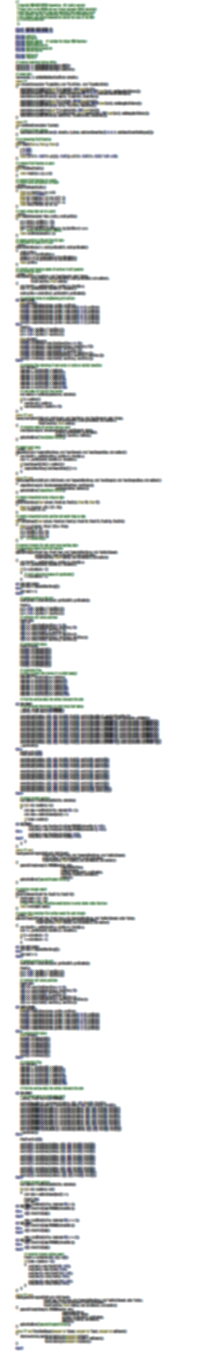
\includegraphics[width=.75in]{images/MCCompareCuda} &
    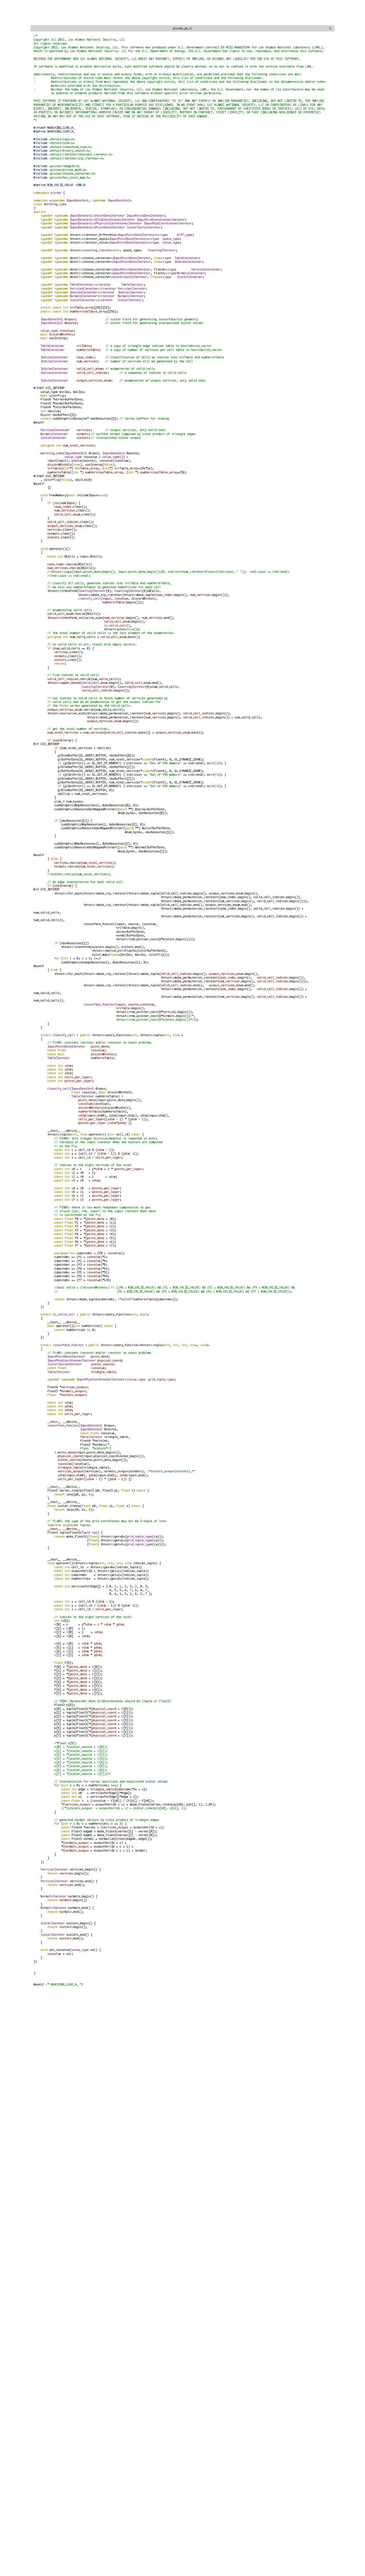
\includegraphics[width=.75in]{images/MCComparePiston} &
    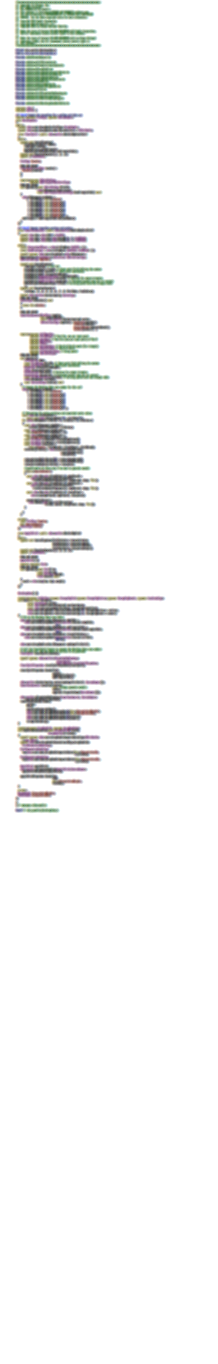
\includegraphics[width=.75in]{images/MCCompareVTKm}
  \end{tabular}
  \caption[Comparison of Marching Cubes implementations.]{Comparison of the
    Marching Cubes algorithm in VTK-m and two other implementations.
    Implementations in VTK-m are simpler, shorter, more general, and easier
    to maintain. (Lines of code (LOC) measurements come from cloc.}
  \label{fig:MCCompare}
\end{figure}

VTK-m simplifies the development of parallel scientific visualization
algorithms by providing a framework of supporting functionality that allows
developers to focus on visualization operations. Consider the listings in
Figure~\ref{fig:MCCompare} that compares the size of the implementations
for the Marching Cubes algorithm in VTK-m with the equivalent algorithms
implemented in the CUDA software development kit reference implementation
and the PISTON visualization library. Because VTK-m internally manages the
parallel distribution of work and data, the VTK-m implementation is shorter
and easier to maintain. Additionally, VTK-m provides data abstractions not
provided by the other libraries that make code written in VTK-m more
versatile.

\begin{didyouknow}
  VTK-m is written in C++ and makes extensive use of templates. The toolkit
  is implemented as a header library, meaning that all the code is
  implemented in header files (with extension \textfilename{.h}) and
  completely included in any code that uses it. This allows the compiler to
  inline and specialize code for better performance.
\end{didyouknow}

\section{How to Use This Guide}

This user's guide is organized into three parts to help guide novice to
advanced users and to provide a convenient reference.
Part~\ref{part:GettingStarted}, Getting Started, provides everything needed
to get up and running with VTK-m. In this part we learn the basics of
reading and writing data files, using filters to process data, and perform
basic rendering to view the results.

Part~\ref{part:Developing}, Developing with VTK-m, dives deeper into the
VTK-m library and provides all the information needed to customize VTK-m's
data structures and support multiple devices. Part~\ref{part:Developing}
also documents how to use VTK-m's framework to develop new or custom
visualization algorithms.

Part~\ref{part:Advanced}, Advanced Customization, exposes the inner
workings of VTK-m and allows you to design new algorithmic structures not
already available. \fix{This might be removed in the first version of the
  book.}

\section{Conventions Used in This Guide}

When documenting the VTK-m API, the following conventions are used.
\begin{itemize}
\item Filenames are printed in a \textfilename{sans serif font}.
\item C++ code is printed in a \textcode{monospace font}.
\item Macros and namespaces from VTK-m are printed in \textnamespace{red}.
\item Identifiers from VTK-m are printed in \textidentifier{blue}.
\item Signatures, described in Chapter~\ref{chap:Worklets}, and the
  tags used in them are printed in \textsignature{green}.
\end{itemize}

This guide provides actual code samples throughout its discussions to
demonstrate their use. These examples are all valid code that can be
compiled and used although it is often the case that code snippets are
provided. In such cases, the code must be placed in a larger context.

\begin{didyouknow}
  In this guide we periodically use these \textbf{Did you know?} boxes to
  provide additional information related to the topic at hand.
\end{didyouknow}

\begin{commonerrors}
  \textbf{Common Errors} blocks are used to highlight some of the common
  problems or complications you might encounter when dealing with the topic
  of discussion.
\end{commonerrors}


  % -*- latex -*-

\chapter{Build and Install \VTKm}
\label{chap:BuildAndInstall}

Before we begin describing how to develop with \VTKm, we have a brief overview of how to build \VTKm, optionally install it on your system, and start your own programs that use \VTKm.


\section{Getting \VTKm}

\VTKm is an open source software product where the code is made freely available.
To get the latest released version of \VTKm, go to the \VTKm releases page:

\begin{quote}
  \url{http://m.vtk.org/index.php/VTK-m_Releases}
\end{quote}

For access to the most recent work, the \VTKm development team provides public anonymous read access to their main source code repository.
The main \VTKm repository on a gitlab instance hosted at Kitware, Inc.
The repository can be browsed from its project web page:

\begin{quote}
  \url{https://gitlab.kitware.com/vtk/vtk-m}
\end{quote}

\index{git|(}

The source code in the \VTKm repository is access through the \textfilename{git} version control tool.
If you have not used \textfilename{git} before, there are several resources available to help you get familiar with it.
Github has a nice setup guide (\url{https://help.github.com/articles/set-up-git}) to help you get up and running quickly.
For more complete documentation, we recommend the \emph{Pro Git} book (\url{https://git-scm.com/book}).

To get a copy of the \VTKm repository, issue a git clone command.

\begin{blankexample}{Cloning the main \VTKm git repository.}
git clone https://gitlab.kitware.com/vtk/vtk-m.git
\end{blankexample}

The git clone command will create a copy of all the source code to your local machine.
As time passes and you want to get an update of changes in the repository, you can do that with the git pull command.

\begin{blankexample}{Updating a git repository with the pull command.}
git pull
\end{blankexample}

\begin{didyouknow}
  The proceeding examples for using git are based on the \textfilename{git} command line tool, which is particularly prevalent on Unix-based and Mac systems.
  There also exist several GUI tools for accessing git repositories.
  These tools each have their own interface and they can be quite different.
  However, they all should have roughly equivalent commands named ``clone'' to download a repository given a url and ``pull'' to update an existing repository.
\end{didyouknow}

\index{git|)}


\section{Configure \VTKm}
\label{sec:ConfigureVTKm}

\index{CMake|(}
\index{CMake!configuration|(}

\VTKm uses a cross-platform configuration tool named CMake to simplify the configuration and building across many supported platforms.
CMake is available from many package distribution systems and can also be downloaded for many platforms from \url{http://cmake.org}.

Most distributions of CMake come with a convenient GUI application (\textfilename{cmake-gui}) that allows you to browse all of the available configuration variables and run the configuration.
Many distributions also come with an alternative terminal-based version (\textfilename{ccmake}), which is helpful when accessing remote systems where creating GUI windows is difficult.

One helpful feature of CMake is that it allows you to establish a build directory separate from the source directory, and the \VTKm project requires that separation.
Thus, when you run CMake for the first time, you want to set the build directory to a new empty directory and the source to the downloaded or cloned files.
The following example shows the steps for the case where the \VTKm source is cloned from the git repository.
(If you extracted files from an archive downloaded from the \VTKm web page, the instructions are the same from the second line down.)

\begin{blankexample}[ex:RunningCMake]{Running CMake on a cloned \VTKm repository.}
git clone https://gitlab.kitware.com/vtk/vtk-m.git
mkdir vtkm-build
cd vtkm-build
cmake-gui ../vtk-m
\end{blankexample}

\begin{figure}[htb]
  \centering
  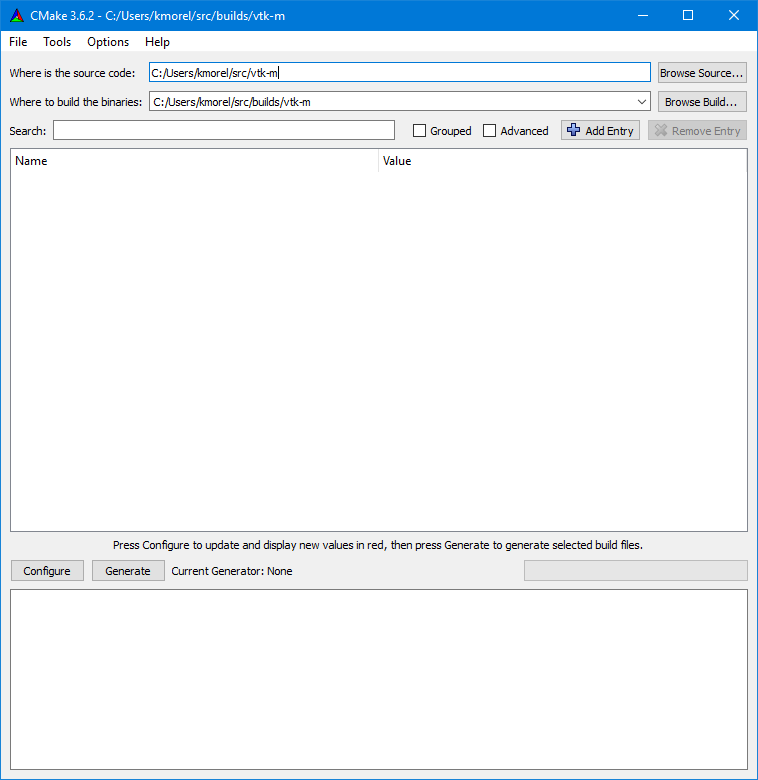
\includegraphics[width=.49\linewidth]{images/CMakeGUIBlank}
  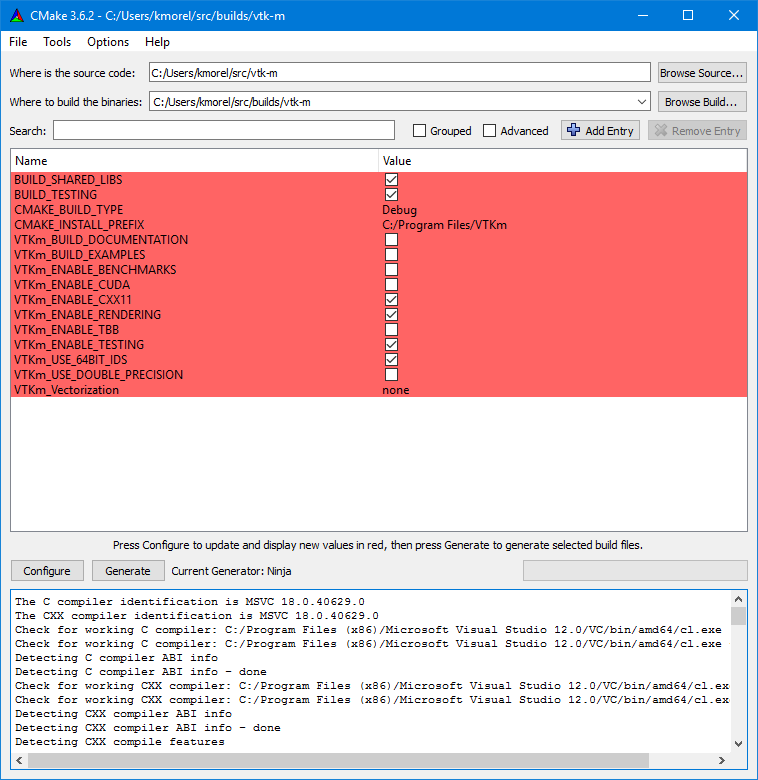
\includegraphics[width=.49\linewidth]{images/CMakeGUI}
  \caption[The CMake GUI configuring the \VTKm project.]{
    The CMake GUI configuring the \VTKm project.
    At left is the initial blank configuration.
    At right is the state after a configure pass.
  }
  \label{fig:CMakeGUI}
\end{figure}

The first time the CMake GUI runs, it initially comes up blank as shown at left in Figure~\ref{fig:CMakeGUI}.
Verify that the source and build directories are correct (located at the top of the GUI) and then click the ``Configure'' button near the bottom.
The first time you run configure, CMake brings up a dialog box asking what generator you want for the project.
This allows you to select what build system or IDE to use (e.g. make, ninja, Visual Studio).
Once you click ``Finish,'' CMake will perform its first configuration.
Don't worry if CMake gives an error about an error in this first configuration process.

\begin{commonerrors}
  Most options in CMake can be reconfigured at any time, but not the compiler and build system used.
  These must be set the first time configure is run and cannot be subsequently changed.
  If you want to change the compiler or the project file types, you will need to delete everything in the build directory and start over.
\end{commonerrors}

After the first configuration, the CMake GUI will provide several configuration options as shown in Figure~\ref{fig:CMakeGUI} on the right.
You now have a chance to modify the configuration of \VTKm, which allows you to modify both the behavior of the compiled \VTKm code as well as find components on your system.
Using the CMake GUI is usually an iterative process where you set configuration options and re-run ``Configure.''
Each time you configure, CMake might find new options, which are shown in red in the GUI.

It is often the case during this iterative configuration process that configuration errors occur.
This can occur after a new option is enabled but CMake does not automatically find the necessary libraries to make that feature possible.
For example, to enable TBB support, you may have to first enable building TBB, configure for TBB support, and then tell CMake where the TBB include directories and libraries are.

Once you have set all desired configuration variables and resolved any CMake errors, click the ``Generate'' button. This will create the build files (such as makefiles or project files depending on the generator chosen at the beginning). You can then close the CMake GUI.

There are a great number of configuration parameters available when running CMake on \VTKm.
The following list contains the most common configuration parameters.

\begin{description}
\item[\cmakevar{BUILD\_SHARED\_LIBS}]
  Determines whether static or shared libraries are built.
\item[\cmakevar{CMAKE\_BUILD\_TYPE}]
  \index{Debug} \index{Release}
  Selects groups of compiler options from categories like Debug and Release.
  Debug builds are, obviously, easier to debug, but they run \emph{much} slower than Release builds.
  Use Release builds whenever releasing production software or doing performance tests.
\item[\cmakevar{CMAKE\_INSTALL\_PREFIX}]
  The root directory to place files when building the install target.
\item[\cmakevar{VTKm\_BUILD\_EXAMPLES}]
  The \VTKm repository comes with an \textfilename{examples} directory.
  This macro determines whether they are built.
\item[\cmakevar{VTKm\_ENABLE\_BENCHMARKS}]
  If on, the \VTKm build includes several benchmark programs.
  The benchmarks are regression tests for performance.
\item[\cmakevar{VTKm\_ENABLE\_CUDA}]
  \index{CUDA}
  Determines whether \VTKm is built to run on CUDA GPU devices.
\item[\cmakevar{VTKm\_ENABLE\_RENDERING}]
  Determines whether to build the rendering library.
\item[\cmakevar{VTKm\_ENABLE\_TBB}]
  Determines whether \VTKm is built to run on multi-core x86 devices using the Intel Threading Building Blocks library.
\item[\cmakevar{VTKm\_ENABLE\_TESTING}]
  If on, the \VTKm build includes building many test programs.
  The \VTKm source includes hundreds of regression tests to ensure quality during development.
\item[\cmakevar{VTKm\_USE\_64BIT\_IDS}]
  If on, then \VTKm will be compiled to use 64-bit integers to index arrays and other lists.
  If off, then \VTKm will use 32-bit integers.
  32-bit integers take less memory but could cause failures on larger data.
\item[\cmakevar{VTKm\_USE\_DOUBLE\_PRECISION}]
  If on, then \VTKm will use double precision (64-bit) floating point numbers for calculations where the precision type is not otherwise specified.
  If off, then single precision (32-bit) floating point numbers are used.
  Regardless of this setting, \VTKm's templates will accept either type.
\end{description}

\index{CMake!configuration|)}
\index{CMake|)}


\section{Building \VTKm}

Once CMake successfully configures \VTKm and generates the files for the build system, you are ready to build \VTKm.
As stated earlier, CMake supports generating configuration files for several different types of build tools.
Make and ninja are common build tools, but CMake also supports building project files for several different types of integrated development environments such as Microsoft Visual Studio and Apple XCode.

The \VTKm libraries and test files are compiled when the default build is invoked.
For example, if \textfilename{Makefile}s were generated, the build is invoked by calling \textfilename{make} in the build directory.
Expanding on Example~\ref{ex:RunningCMake}

\begin{blankexample}[ex:RunningMake]{Using \textfilename{make} to build \VTKm.}
git clone https://gitlab.kitware.com/vtk/vtk-m.git
mkdir vtkm-build
cd vtkm-build
cmake-gui ../vtk-m
make -j
make test
make install
\end{blankexample}

\begin{didyouknow}
  The \textfilename{Makefile}s and other project files generated by CMake support parallel builds, which run multiple compile steps simultaneously.
  On computers that have multiple processing cores (as do almost all modern computers), this can significantly speed up the overall compile.
  Some build systems require a special flag to engage parallel compiles.
  For example, \textfilename{make} requires the \textfilename{-j} flag to start parallel builds as demonstrated in Example~\ref{ex:RunningMake}.
\end{didyouknow}

\begin{commonerrors}
  CMake allows you to switch between several types of builds including default, Debug, and Release.
  Programs and libraries compiled as release builds can run \emph{much} faster than those from other types of builds.
  Thus, it is important to perform Release builds of all software released for production or where runtime is a concern.
  Some integrated development environments such as Microsoft Visual Studio allow you to specify the different build types within the build system.
  But for other build programs, like \textfilename{make}, you have to specify the build type in the \cmakevar{CMAKE\_BUILD\_TYPE} CMake configuration variable, which is described in Section~\ref{sec:ConfigureVTKm}.
\end{commonerrors}

CMake creates several build ``targets'' that specify the group of things to build.
The default target builds all of \VTKm's libraries as well as tests, examples, and benchmarks if enabled.
The \textfilename{test} target executes each of the \VTKm regression tests and verifies they complete successfully on the system.
The \textfilename{install} target copies the subset of files required to use \VTKm to a common installation directory.
The \textfilename{install} target may need to be run as an administrator user if the installation directory is a system directory.

\begin{didyouknow}
  A good portion of \VTKm is a header-only library, which does not need to be built in a traditional sense.
  However, \VTKm contains a significant amount of tests to ensure that the header code does compile and run correctly on a given system.
  If you are not concerned with testing a build on a given system, you can turn off building the testing, benchmarks, and examples using the CMake configuration variables described in Section~\ref{sec:ConfigureVTKm}.
  This can shorten the \VTKm compile time.
\end{didyouknow}


\section{Linking to \VTKm}
\label{sec:LinkingToVTKm}

Ultimately, the value of \VTKm is the ability to link it into external projects that you write.
The header files and libraries installed with \VTKm are typical, and thus you can link \VTKm into a software project using any type of build system.
However, \VTKm comes with several CMake configuration files that simplify linking \VTKm into another project that is also managed by CMake.
Thus, the documentation in this section is specifically for finding and configuring \VTKm for CMake projects.

\index{CMake|(}
\index{CMake!VTK-m package|(}
\index{VTK-m CMake package|(}

\VTKm can be configured from an external project using the \textcode{find\_package} CMake function.
The behavior and use of this function is well described in the CMake documentation.
The first argument to \textcode{find\_package} is the name of the package, which in this case is \textcode{VTKm}.
CMake configures this package by looking for a file named \textfilename{VTKmConfig.cmake}, which will be located in the \textfilename{lib} directory of the install or build of \VTKm.
The configurable CMake variable \cmakevar{VTKm\_DIR} can be set to the directory that contains this file.

\begin{didyouknow}
  The CMake \textcode{find\_package} function also supports several features not discussed here including specifying a minimum or exact version of \VTKm and turning off some of the status messages.
  See the CMake documentation for more details.
\end{didyouknow}

\index{CMake!VTK-m package!components|(}
\index{VTK-m CMake package!components|(}

\newcommand*{\cmakecomponent}[1]{%
  \textsf{#1}%
  \index{#1}%
  \index{CMake!VTK-m package!#1}%
  \index{VTK-m CMake package!components!#1}}

The CMake package for VTK-m is broken down into components that let you load particular features of VTK-m.
Package components can be specified with the \textcode{COMPONENTS} and \textcode{OPTIONAL\_COMPONENTS} arguments to the \textcode{find\_package} function.
The following example demonstrates using \textcode{find\_package} to find the \VTKm package that requires the \cmakecomponent{Serial} backend as well as the \cmakecomponent{Rendering} and \cmakecomponent{OpenGL} features as well as optionally using the \cmakecomponent{TBB} and \cmakecomponent{CUDA} backends.

\begin{blankexample}{Loading \VTKm configuration from an external CMake project.}
find_package(VTKm REQUIRED
  COMPONENTS Serial OpenGL Rendering
  OPTIONAL_COMPONENTS TBB CUDA
  )
\end{blankexample}

The following components are available.
Many of the features for these components are described elsewhere within this book.

\begin{description}
\item[\cmakecomponent{Base}]
  The ``base'' configuration required for using any part of \VTKm.
  This component is loaded automatically even if no components are specified in \textcode{find\_package}.
\item[\cmakecomponent{Serial}]
  The serial backend for \VTKm, which is useful for debugging and when no other backend is available.
\item[\cmakecomponent{OpenGL}]
  Support for the integration of OpenGL features with \VTKm.
\item[\cmakecomponent{OSMesa}]
  Support for creating off screen canvases using the OSMesa library.
\item[\cmakecomponent{EGL}]
  Support for creating off screen canvases using the EGL library.
\item[\cmakecomponent{GLFW}]
  A convenience component that loads the necessary configuration to use the GLFW library, which provides a cross-platform interface for creating OpenGL windows.
\item[\cmakecomponent{GLUT}]
  A convenience component that loads the necessary configuration to use the GLUT library, which provides a cross-platform interface for creating OpenGL windows.
\item[\cmakecomponent{Interop}]
  Support for transferring \VTKm array data directly to OpenGL objects.
\item[\cmakecomponent{Rendering}]
  Use of the lightweight \VTKm rendering library, which provides basic rendering of \VTKm data objects.
\item[\cmakecomponent{TBB}]
  The Intel Threading Building Blocks (TBB) backend for \VTKm, which uses multiple cores and threads for parallel processing.
\item[\cmakecomponent{CUDA}]
  The CUDA backend for \VTKm, which uses GPU processors for parallel processing.
\end{description}

\index{VTK-m CMake package!components|)}
\index{CMake!VTK-m package!components|)}

\newcommand*{\cmakevtkmpackagevariable}[1]{%
  \textsf{#1}%
  \index{#1}%
  \index{CMake!VTK-m package!#1}%
  \index{VTK-m CMake package!variables!#1}}

After the \textcode{find\_package} function completes, C++ libraries and executables can be creating using the configuration variables defined.
The following is a simple example of creating an executable.

\begin{blankexample}{Loading \VTKm configuration from an external CMake project.}
find_package(VTKm REQUIRED
  COMPONENTS Serial OpenGL Rendering
  OPTIONAL_COMPONENTS TBB CUDA
  )

add_executable(myprog myprog.cxx)
target_include_directories(myprog PRIVATE ${VTKm_INCLUDE_DIRS})
target_link_libraries(myprog ${VTKm_LIBRARIES})
target_compile_options(myprog PRIVATE ${VTKm_COMPILE_OPTIONS})
\end{blankexample}

\begin{commonerrors}
  It is not sufficient to just call \textcode{find\_package} to compile code using \VTKm.
  You must also use the \cmakevtkmpackagevariable{VTKm\_INCLUDE\_DIRS} and \cmakevtkmpackagevariable{VTKm\_LIBRARIES} CMake variables to configure the compiler to load \VTKm's components.
  (Although technically not required, it is highly advisable to also use the \cmakevtkmpackagevariable{VTKm\_COMPILE\_OPTIONS} variable as well.) 
\end{commonerrors}

\index{CMake!VTK-m package!variables|(}
\index{VTK-m CMake package!variables|(}

The following is a list of all the CMake variables defined when the \textcode{find\_package} function completes.

\begin{description}
\item[\cmakevtkmpackagevariable{VTKm\_FOUND}]
  Set to true if the \VTKm CMake package, all its dependent packages, and all the specified components were successfully configured.
  If \textcode{find\_package} was not called with the \textcode{REQUIRED} option, then this variable should be checked before attempting to use \VTKm.
\item[\cmakevtkmpackagevariable{VTKm\_{\it{}\textless{}component\_name\textgreater{}}\_FOUND}]
  For each component specified in the \textcode{find\_package} call, one of these variables will be defined as true or false depending on whether the component successfully loaded.
  For components specified as an \textcode{OPTIONAL\_COMPONENTS} argument, the \cmakevtkmpackagevariable{VTKm\_FOUND} might still be true (because all required components succeeded) while the associated \cmakevtkmpackagevariable{VTKm\_{\it{}\textless{}component\_name\textgreater{}}\_FOUND} could be false if that specific component failed to load.
\item[\cmakevtkmpackagevariable{VTKm\_INCLUDE\_DIRS}]
  Contains a list of all directories that need to be specified to properly include \VTKm header files.
  These also include the directories needed for header files that \VTKm depends on and specified components.
  Targets should use the \textcode{target\_include\_directories} CMake function to add this list of directories to the compile commands.
\item[\cmakevtkmpackagevariable{VTKm\_LIBRARIES}]
  Contains a list of all requested \VTKm libraries and component libraries.
  Targets should use the \textcode{target\_link\_libraries} CMake function to add this list of libraries to the link commands.
\item[\cmakevtkmpackagevariable{VTKm\_COMPILE\_OPTIONS}]
  Contains a string of options that \VTKm suggests to add to the compiler.
  Targets should use the \textcode{target\_compile\_options} CMake function to add this list of options to the compile commands.
\end{description}

\index{VTK-m CMake package!variables|)}
\index{CMake!VTK-m package!variables|)}

\index{VTK-m CMake package|)}
\index{CMake!VTK-m package|)}
\index{CMake|)}


  \chapter{File I/O}
\label{chap:FileIO}

\index{I/O|(}
\index{file~I/O|(}

Before VTK-m can be used to process data, data need to be loaded into the
system. VTK-m comes with a basic file I/O package to get started developing
very quickly. All the file I/O classes are declared under the \vtkmio{}
namespace.

\begin{didyouknow}
  Files are just one of many ways to get data in and out of VTK-m. In
  Part~\ref{part:Using} we explore efficient ways to define VTK-m data
  structures. In particular, Section~\ref{sec:DataSets:Building} describes
  how to build VTK-m data set objects and
  Section~\ref{sec:ArrayHandle:Adapting} documents how to adapt data
  structures defined in other libraries to be used directly in VTK-m.
\end{didyouknow}

\section{Readers}

\index{file~I/O!read|(}
\index{read~file|(}

All reader classes provided by VTK-m are located in the \vtkmioreader{}
namespace. The general interface for each reader class is to accept a
filename in the constructor and to provide a \textcode{ReadDataSet} method
to load the data from disk.

The data in the file are returned in a \vtkmcont{DataSet} object.
Chapter~\ref{chap:DataSets} provides much more details about the contents of
a data set object, but for now we treat \textidentifier{DataSet} as an
opaque object that can be passed around readers, writers, filters, and
rendering units.

\subsection{Legacy VTK File Reader}

Legacy VTK files are a simple open format for storing visualization data.
These files typically have a \textfilename{.vtk} extension. Legacy VTK
files are popular because they are simple to create and read and are
consequently supported by a large number of tools. The format of legacy VTK
files is well documented in \textit{The VTK User's Guide}\footnote{A free
  excerpt describing the file format is available at
  \url{http://www.vtk.org/Wiki/File:VTK-File-Formats.pdf}.}. Legacy VTK
files can also be read and written with tools like ParaView and VisIt.

Legacy VTK files can be read using the \vtkmioreader{VTKDataSetReader}
class. The constructor for this class takes a string containing the
filename. The \textcode{ReadDataSet} method reads the data from the
previously indicated file and returns a \vtkmcont{DataSet} object, which
can be used with filters and rendering.

\vtkmlisting{Reading a legacy VTK file.}{VTKDataSetReader.cxx}

\index{read~file|)}
\index{file~I/O!read|)}

\section{Writers}

\index{file~I/O!write|(}
\index{write~file|(}

All writer classes provided by VTK-m are located in the \vtkmiowriter{}
namespace. The general interface for each writer class is to accept a
filename in the constructor and to provide a \textcode{WriteDataSet} method
to save data to the disk. The \textcode{WriteDataSet} method takes a
\vtkmcont{DataSet} object as an argument, which contains the data to write
to the file.

\subsection{Legacy VTK File Writer}

\index{write~file|)}
\index{file~I/O!write|)}

Legacy VTK files can be written using the \vtkmiowriter{VTKDataSetWriter}
class. The constructor for this class takes a string containing the
filename. The \textcode{WriteDataSet} method takes a \vtkmcont{DataSet}
object and writes its data to the previously indicated file.

\vtkmlisting{Writing a legacy VTK file.}{VTKDataSetWriter.cxx}

\index{file~I/O|)}
\index{I/O|)}


  % -*- latex -*-

\chapter{Provided Filters}
\label{chap:ProvidedFilters}

\index{filter|(}

Filters are functional units that take data as input and write new data as
output. Filters operate on \vtkmcont{DataSet} objects, which are introduced
with the file I/O operations in Chapter~\ref{chap:IO} and are described in
more detail in Chapter~\ref{chap:DataSet}. For now we treat
\textidentifier{DataSet} mostly as an opaque object that can be passed
around readers, writers, filters, and rendering units.

\begin{didyouknow}
  The structure of filters in VTK-m is significantly simpler than their
  counterparts in VTK. VTK filters are arranged in a dataflow network
  (a.k.a. a visualization pipeline) and execution management is handled
  automatically. In contrast, VTK-m filters are simple imperative units,
  which are simply called with input data and return output data.
\end{didyouknow}

VTK-m comes with several filters ready for use, and in this chapter we will
give a brief overview of these filters. We group filters based on the type
of operation that they do and the shared interfaces that they have. Later
Part~\ref{part::Developing} describes the necessary steps in creating new
filters in VTK-m.


\section{Field Filters}

\index{filter!field|(}
\index{field~filter|(}

Every \vtkmcont{DataSet} object contains a list of \index{field}
\keyterm{fields}. A field describes some numerical value associated with
different parts of the data set in space. Fields often represent physical
properties such as temperature, pressure, or velocity. \keyterm{Field
  filters} are a class of filters that generate a new field. These new
fields are typically derived from one or more existing fields or point
coordinates on the data set. For example, mass, volume, and density are
interrelated, and any one can be derived from the other two.

All field filters contain an \textcode{Execute} method that takes two
arguments. The first argument is a \vtkmcont{DataSet} object with the input
data. The second argument specifies the field from which to derive a new
field. The field can be specified as either a string naming a field in the
input \textidentifier{DataSet} object, as a \vtkmcont{Field} object, or as
a coordinate system (typically retrived from a \textidentifier{DataSet}
object with the \textcode{GetCoordianteSystem} method). See Sections
\ref{sec:DataSets:Fields} and \ref{sec:DataSets:CoordinateSystems} for more
information on fields and coordinate systems, respectively.

Field filters often need more information than just a data set and a field.
Any additional information is provided using methods in the filter class
that changes the state. These methods are called before \textcode{Execute}.
One such method that all field filters have is
\textcode{SetOutputFieldName}, which specifies the name assigned to the
generated field. If not specified, then the filter will use a default name.

The \textcode{Execute} method returns a \vtkmfilter{ResultField} object,
which contains the state of the execution and the data generated. A
\textidentifier{ResultField} object has the following methods.

\begin{description}
\item[\textcode{IsValid}] Returns a \textcode{bool} value specifying
  whether the execution completed successfully. If \textcode{true}, then
  the execution was successful and the data stored in the
  \textidentifier{ResultField} is valid. If \textcode{false}, then the
  execution failed.
\item[\textcode{GetDataSet}] Returns a \textidentifier{DataSet} containing
  the results of the execution. The data set returned is a shallow copy of
  the input data with the generated field added.
\item[\textcode{GetField}] Returns the field information in a
  \vtkmcont{Field} object. Field objects are described in
  Section~\ref{sec:DataSets:Fields}.
\item[\textcode{FieldAs}] Given a \vtkmcont{ArrayHandle} object, allocates
  the array and copies the generated field data into it.
\end{description}

The following example provides a simple demonstration of using a field
filter. It specifically uses the point elevation filter, which is one of
the field filters.

\vtkmlisting[ex:PointElevation]{Using \textidentifier{PointElevation}, which is a field filter.}{PointElevation.cxx}

\subsection{Cell Average}

\index{cell~average|(}
\index{average|(}

\vtkmfilter{CellAverage} is the cell average filter. It will take a data
set with a collection of cells and a field defined on the points of the
data set and create a new field defined on the cells. The values of this
new derived field are computed by averaging the values of the input field
at all the incident points. This is a simple way to convert a point field
to a cell field. Both the input data set and the input field are specified
as arguments to the \textcode{Execute} method.

The default name for the output cell field is the same name as the input
point field. The name can be overridden using the
\textcode{SetOutputFieldName} method.

In addition the standard \textcode{SetOutputFieldName} and
\textcode{Execute} methods, \textidentifier{CellAverage} provides the
following methods.

\begin{description}
\item[\textcode{SetActiveCellSet}] Sets the index for the cell set to use
  from the \textidentifier{DataSet} provided to the \textcode{Execute}
  method. The default index is 0, which is the first cell set. If you want
  to set the active cell set by name, you can use the
  \textidentifier{GetCellSetIndex} method on the \textidentifier{DataSet}
  object that will be used with \textcode{Execute}.
\item[\textcode{GetActiveCellSetIndex}] Returns the index to be used when
  getting a cell set from the \textidentifier{DataSet} passed to
  \textcode{Execute}. Set with \textcode{SetActiveCellSet}.
\end{description}

\index{average|}
\index{cell~average|)}

\subsection{Point Elevation}

\index{point~elevation|(}
\index{elevation|(}

\vtkmfilter{PointElevation} computes the ``elevation'' of a field of point
coordinates in space. The filter will take a data set and a field of 3
dimensional vectors and compute the distance along a line defined by a low
point and a high point. Any point in the plane touching the low point and
perpendicular to the line is set to the minimum range value in the
elevation whereas any point in the plane touching the high point and
perpendicular to the line is set to the maximum range value. All other
values are interpolated linearly between these two planes. This filter is
commonly used to compute the elevation of points in some direction, but can
be repurposed for a variety of measures.

The input field (or coordinate system) is specified as the second argument
to the \textcode{Execute} method. A \vtkmcont{DataSet} that is expected to
contain the field is also given but is otherwise unused.
Example~\ref{ex:PointElevation} gives a demonstration of the elevation
filter.

The default name for the output field is ``elevation'', but that can be
overridden using the \textcode{SetOutputFieldName} method.

In addition to the standard \textcode{SetOutputFieldName} and
\textcode{Execute} methods, \textidentifier{PointElevation} provides the
following methods.

\begin{description}
\item[\textcode{SetLowPoint}/\textcode{SetHighPoint}] This pair of methods
  is used to set the low and high points, respectively, of the elevation.
  Each method takes three floating point numbers specifying the $x$, $y$,
  and $z$ components of the low or high point.
\item[\textcode{SetRange}] Sets the range of values to use for the output
  field. This method takes two floating point numbers specifying the low
  and high values, respectively.
\end{description}

\index{elevation|)}
\index{point~elevation|)}

\index{field~filter|)}
\index{filter!field|)}


\section{Data Set Filters}

\index{filter!data~set|(}
\index{data~set~filter|(}

\keyterm{Data set filters} are a class of filters that generate a new data
set with a new topology. This new topology is typically derived from an
existing data set. For example, a data set can be significantly altered by
adding, removing, or replacing cells.

All data set filters contain an \textcode{Execute} method that takes one
argument: a \vtkmcont{DataSet} object with the input data.

Some data set filters need more information that just a data set when
executing. Any additional information is provided using methods in the
filter class that changes the state. These methods are called before
\textcode{Execute}. One such method that all data set filters have is
\textcode{SetActiveCellSet}, which selects which cell set in the input
\textidentifier{DataSet} to operate on. Likewise,
\textcode{SetActiveCoordinateSystem} selects which coordinate system to
operate on. By default, the filter will operate on the first cell set and
coordinate system. (See Sections \ref{sec:DataSets:CellSets} and
\ref{sec:DataSets:CoordinateSystems} for more information about cell sets
and coordinate systems, respectively.)

The \textcode{Execute} method returns a \vtkmfilter{ResultDataSet} object,
which contains the state of the execution and the data generated. A
\textidentifier{ResultDataSet} object has the following methods.

\begin{description}
\item[\textcode{IsValid}] Returns a \textcode{bool} value specifying
  whether the execution completed successfully. If \textcode{true}, then
  the execution was successful and the data stored in the
  \textidentifier{ResultField} is valid. If \textcode{false}, then the
  execution failed.
\item[\textcode{GetDataSet}] Returns a \textidentifier{DataSet} containing
  the results of the execution.
\end{description}

Because the new data set is derived from existing data, it can often
inherit field information from the original data. All data set filters also
contain a \textcode{MapFieldOntoOutput} method to map fields from the
output to the input. This method takes two arguments. The first argument is
the \textidentifier{ResultDataSet} object returned from the last call to
\textcode{Execute}. The second argument is a \vtkmcont{Field} object that
comes from the input. \textcode{MapFieldOntoOutput} returns a
\textcode{bool} that is true if the field was successfully mapped and added
to the output data set in the \textidentifier{ResultDataSet} object.

\begin{commonerrors}
  Not all data set filters support the mapping of all input fields to the
  output. If the mapping is not supported, \textcode{MapFieldOntoOutput}
  will simply return false.
\end{commonerrors}

The following example provides a simple demonstration of using a data set
filter. It specifically uses the vertex clustering filter, which is one of
the data set filters.

\vtkmlisting[ex:VertexClustering]{Using \textidentifier{VertexClustering},
  which is a data set filter.}{VertexClustering.cxx}

\subsection{External Faces}

\index{external~faces|(}
\index{face!external|(}

\vtkmfilter{ExternalFaces} is a filter that extracts all the external faces
from a polyhedral data set. An external face is any face that is on the
boundary of a mesh. Thus, if there is a hole in a volume, the boundary of
that hole will be considered external. More formally, an external face is
one that belongs to only one cell in a mesh.

\begin{commonerrors}
  The current implementation of the external faces filter only supports
  tetrahedron cell cells. Future versions will support general 3D cell
  shapes. \fix{Remove this when the code is updated.}
\end{commonerrors}

The external faces filter has no extra methods beyond the base methods of
data set filters (such as \textcode{Execute} and
\textcode{MapFieldOntoOutput}) because it requires no further metadata for
its operations.

\index{face!external|)}
\index{external~faces|)}

\index{data~set~filter|)}
\index{filter!data~set|)}

\subsection{Vertex Clustering}

\index{vertex~clustering|(}
\index{surface~simplification|(}

\vtkmfilter{VertexClustering} is a filter that simplifies a polygonal mesh.
It does so by dividing space into a uniform grid of bin and then merges
together all points located in the same bin. The smaller the dimensions of
this binning grid, the fewer polygons will be in the output cells and the
coarser the representation. This surface simplification is an important
operation to support \index{level~of~detail}\index{LOD}level of detail (LOD)
rendering in visualization applications. Example~\ref{ex:VertexClustering}
provides a demonstration of the vertex clustering filter.

In addition to the standard \textcode{Execute},
\textcode{MapFieldOntoOutput}, and other methods,
\textidentifier{VertexClustering} provides the following methods.

\begin{description}
\item[\textcode{SetNumberOfDivisions}] Set the dimensions of the uniform
  grid that establishes the bins used for clustering. Setting smaller
  numbers of dimensions produces a smaller output, but with a coarser
  representation of the surface. The dimensions are provided as a
  \vtkm{Id3}.
\item[\textcode{GetNumberOfDimensions}] Returns the number of dimensions
  used for binning. The dimensions are returned as a \vtkm{Id3}.
\end{description}

\index{surface~simplification|}
\index{vertex~clustering|)}


\section{Data Set and Field Filters}

\index{filter!data~set~with~field|(}
\index{data~set~with~filter|(}

\keyterm{Data set and field filters} are a class of filters that generate a
new data set with a new topology. This new topology is derived from an
existing data set and at least one of the fields in the data set. For
example, a field might determine how each cell is culled, clipped, or
sliced.

All data set and field filters contain an \textcode{Execute} method that
takes two arguments. The first argument is a \vtkmcont{DataSet} object with
the input data. The second argument specifies the field from which to
derive a new field. The field can be specified as either a string naming a
field in the input \textidentifier{DataSet} object, as a \vtkmcont{Field}
object, or as a coordinate system (typically retrieved from a
\textidentifier{DataSet} object with the \textcode{GetCoordianteSystem}
method). See Sections \ref{sec:DataSets:Fields} and
\ref{sec:DataSets:CoordinateSystems} for more information on fields and
coordinate systems, respectively.

Some data set filters need more information that just a data set when
executing. Any additional information is provided using methods in the
filter class that changes the state. These methods are called before
\textcode{Execute}. One such method that all data set filters have is
\textcode{SetActiveCellSet}, which selects which cell set in the input
\textidentifier{DataSet} to operate on. Likewise,
\textcode{SetActiveCoordinateSystem} selects which coordinate system to
operate on. By default, the filter will operate on the first cell set and
coordinate system. (See Sections \ref{sec:DataSets:CellSets} and
\ref{sec:DataSets:CoordinateSystems} for more information about cell sets
and coordinate systems, respectively.)

The \textcode{Execute} method returns a \vtkmfilter{ResultDataSet} object,
which contains the state of the execution and the data generated. A
\textidentifier{ResultDataSet} object has the following methods.

\begin{description}
\item[\textcode{IsValid}] Returns a \textcode{bool} value specifying
  whether the execution completed successfully. If \textcode{true}, then
  the execution was successful and the data stored in the
  \textidentifier{ResultField} is valid. If \textcode{false}, then the
  execution failed.
\item[\textcode{GetDataSet}] Returns a \textidentifier{DataSet} containing
  the results of the execution.
\end{description}

Because the new data set is derived from existing data, it can often
inherit field information from the original data. All data set filters also
contain a \textcode{MapFieldOntoOutput} method to map fields from the
output to the input. This method takes two arguments. The first argument is
the \textidentifier{ResultDataSet} object returned from the last call to
\textcode{Execute}. The second argument is a \vtkmcont{Field} object that
comes from the input. \textcode{MapFieldOntoOutput} returns a
\textcode{bool} that is true if the field was successfully mapped and added
to the output data set in the \textidentifier{ResultDataSet} object.

\begin{commonerrors}
  Not all data set filters support the mapping of all input fields to the
  output. If the mapping is not supported, \textcode{MapFieldOntoOutput}
  will simply return false.
\end{commonerrors}

The following example provides a simple demonstration of using a data set
and field filter. It specifically uses the Marching Cubes filter, which is
one of the data set and field filters.

\vtkmlisting[ex:MarchingCubes]{Using \textidentifier{MarchingCubes},
  which is a data set and field filter.}{MarchingCubes.cxx}

\subsection{Marching Cubes}

\index{filter!Marching~Cubes|(}
\index{filter!contour|(}
\index{filter!isosurface|(}
\index{Marching~Cubes|(}
\index{contour|(}
\index{isosurface|(}

\keyterm{Contouring} is one of the most fundamental filters in scientific
visualization. A contour is the locus where a field is equal to a
particular value. A topographic map showing curves of various elevations
often used when hiking in hilly regions is an example of contours of an
elevation field in 2 dimensions. Extended to 3 dimensions, a contour gives
a surface. Thus, a contour is often called an \keyterm{isosurface}.
Marching Cubes is a well know algorithm for computing contours and is
implemented by \vtkmfilter{MarchingCubes}. Example~\ref{ex:MarchingCubes}
provides a demonstration of the Marching Cubes filter.

In addition to the standard \textcode{Execute},
\textcode{MapFieldOntoOutput}, and other methods,
\textidentifier{MarchingCubes} provides the following methods.

\begin{description}
\item[\textcode{SetIsoValue}] Provide the value on which to extract the
  contour. The contour will be the surface where the field (provided to
  \textcode{Execute}) is equal to this value.
\item[\textcode{GetIsoValue}] Retrieve the currently set iso value.
\item[\textcode{SetMergeDuplicatePoints}] Sets a Boolean flag to determine
  whether coincident points in the data set should be merged. Because the
  Marching Cubes filter (like all filters in VTK-m) runs in parallel,
  parallel threads can (and often do) create duplicate versions of points.
  When this flag is set to true, a secondary operation will find all
  duplicated points and combine them together.
\item[\textcode{GetMergeDuplicatePoints}] Returns the merge duplicate
  points flag.
\item[\textcode{SetGenerateNormals}] Sets a Boolean flag to determine
  whether to generate normal vectors for the surface. Normals are used in
  shading calculations during rendering and can make the surface appear
  more smooth. Generated normals are based on the gradient of the field
  being contoured.
\item[\textcode{GetGenerateNormals}] Returns the generate normals flag.
\end{description}

\index{isosurface|)}
\index{contour|)}
\index{Marching~Cubes|)}
\index{filter!isosurface|)}
\index{filter!contour|)}
\index{filter!Marching~Cubes|)}

\subsection{Threshold}

\index{filter!threshold|(}
\index{threshold|(}

A threshold operation removes topology elements from a data set that do not
meet a specified criterion. The \vtkmfilter{Threshold} filter removes all
cells where the field (provided to \textcode{Execute}) is not between a
range of values.

In addition to the standard \textcode{Execute},
\textcode{MapFieldOntoOutput}, and other methods,
\textidentifier{Threshold} provides the following methods.

\begin{description}
\item[\textcode{SetLowerThreshold}] Sets the lower scalar value. Any cells
  where the scalar field is less than this value are removed.
\item[\textcode{SetUpperThreshold}] Sets the upper scalar value. Any cells
  where the scalar field is more than this value are removed.
\item[\textcode{GetLowerThreshold}] Returns the lower threshold value.
\item[\textcode{GetUpperThreshold}] Returns the upper threshold value.
\end{description}

\index{threshold|)}
\index{filter!threshold|)}

\index{data~set~with~filter|)}
\index{filter!data~set~with~field|)}


\index{filter|)}


  %-*- latex -*-

\chapter{Rendering}
\label{chap:Rendering}

\index{rendering|(}

Rendering, the generation of images from data, is a key component to
visualization. To assist with rendering, VTK-m provides a rendering package
to produce imagery from data.

The rendering package in VTK-m is not intended to be a fully featured
rendering system or library. Rather, it is a lightweight rendering package
with two primary use cases:
\begin{enumerate}
\item New users getting started with VTK-m need a ``quick and dirty''
  render method to see their visualization results.
\item In situ visualization that integrates VTK-m with a simulation or
  other data-generation system might need a lightweight rendering method.
\end{enumerate}

Both of these use cases require just a basic rendering platform. Because
VTK-m is designed to be integrated into larger systems, it does not aspire
to have a fully featured rendering system.

\begin{didyouknow}
  VTK-m's big sister toolkit VTK is already integrated with VTK-m and has
  its own fully featured rendering system. If you need more rendering
  capabilities than what VTK-m provides, you can leverage VTK instead.
\end{didyouknow}

\section{Creating a Rendering Canvas}
\label{sec:Canvas}

\index{rendering!canvas|(}
\index{canvas|(}

The first step in using VTK-m's rendering package is to create a
\keyterm{canvas}, which is managed by \vtkmrendering{Canvas} and its
subclasses. The \textidentifier{Canvas} object manages the frame buffers
and the rendering context.

Subclasses of \textidentifier{Canvas} establish a context for different
rendering systems. Currently, there are two main subclasses: one for using
OpenGL rendering (\vtkmrendering{CanvasGL}) and one for using built in
ray tracing (\vtkmrendering{CanvasRayTracer}).

\subsection{Creating an OpenGL Context with GLUT}

\index{rendering!GLUT|(}
\index{rendering!OpenGL|(}
\index{canvas!GLUT|(}
\index{canvas!OpenGL|(}
\index{GLUT|(}
\index{OpenGL|(}

One feature that is notably (and intentionally) missing from the VTK-m
rendering package is the ability to open a rendering window or build a
graphical user interface. However, VTK-m can use an OpenGL context
established elsewhere to perform rendering. OpenGL is a widely-accepted
rendering library supported by all hardware vendors on pretty much all
computing platforms. It is also extensively used by many applications
performing rendering, particularly scientific visualization applications.

Once an OpenGL rendering context is established, it can be used by VTK-m by
simply creating a \vtkmrendering{CanvasGL}. When created,
\textidentifier{CanvasGL} will find the current OpenGL context, query its
size, and ready the VTK-m rendering system to use it.

Unfortunately, creating a window with an OpenGL context is platform
dependent. There are numerous libraries available that provide the ability
to create an OpenGL window that have been ported to many platforms (such as
MS Windows, Unix, and Mac OSX). One such library is \keyterm{GLUT}.

GLUT is a very simple utility toolkit that provides a basic mechanism for
creating a window with an OpenGL context. It additionally provides simple
user interface features to capture keystrokes and mouse movements. For the
purposes of demonstration, we will provide examples that use GLUT to make a
simple interactive rendering application.

\begin{didyouknow}
  We are demonstrating rendering with GLUT for illustrative purposes only.
  VTK-m is not directly associated with GLUT: It neither comes with GLUT
  nor depends on GLUT. You are welcome to follow these boilerplate
  examples, or you can integrate with another rendering system of your
  choosing.
\end{didyouknow}

This section provides a terse description of getting a GLUT application up
and running. This is not meant to be a thorough description of the GLUT
library. There are other resources that document using the GLUT API, the
most complete of which is the book \emph{OpenGL Programming for the X
  Window System} by Mark J. Kilgard. The information provided here is just
enough to get you started.

\begin{commonerrors}
  Although distributed for free, the original GLUT library was not released
  as open source. Unfortunately, the GLUT copyright holders are not as
  actively developing GLUT as they once were, and consequently some systems
  are declaring GLUT as deprecated. However, there some newer projects like
  FreeGLUT and OpenGLUT that are open source, that are being more actively
  developed, and that are drop in replacements to the original GLUT
  library. There are also alternative libraries such as GLFW that have
  similar capabilities but a different API. These are not documented here,
  but are worth investigating if GLUT does not work for you.
\end{commonerrors}

The first call made to the GLUT library should be to the function
\textcode{glutInit}, which takes as arguments the \textcode{argc} and
\textcode{argv} arguments passed to the \textcode{main} C function.
\textcode{glutInit} will find any window-system specific flags (such as
\textcode{-display}), use them to initialize the windowing system, and
strip them from the arguments.

Next, the parameters for the window to be created should be established.
The function \textcode{glutInitWindowSize} takes the width and the height
of the renderable space in the window. The function
\textcode{glutInitDisplayMode} takes a mask of flags that are or-ed
together to specify the capabilities of the window. We recommend the flags
\textcode{GLUT\_RGBA}, \textcode{GLUT\_DOUBLE}, \textcode{GLUT\_ALPHA}, and
\textcode{GLUT\_DEPTH}. Once these are specified a call to
\textcode{glutCreateWindow} will create a window and initialize the OpenGL
context. \textcode{glutCreateWindow} takes a string for an argument that is
used in the title bar of the window.

\vtkmlisting{Initializing the GLUT library and creating a window to render into.}{InitializeGlut.cxx}

\index{GLUT!callbacks|(}

Apart from the initial setup, most of the interaction with the GLUT
library happens through callbacks. As part of its initialization, an
application provides function pointers to GLUT. GLUT then calls these
provided functions when certain events happen. GLUT supports many callbacks
for different types of events. Here is the small set of callbacks we use in
our small example.

\begin{description}
\item[\textcode{glutDisplayFunc}] The display function is called when the
  window needs to be redrawn. The callback should issue the appropriate
  OpenGL rendering calls and then call \textcode{glutSwapBuffers} to show
  the result.
\item[\textcode{glutReshapeFunc}] The reshape function is called whenever
  the window is resized. The callback is given the width and height of the
  new rendering window.
\item[\textcode{glutMouseFunc}] The mouse button function is called
  whenever a mouse button is pressed or released. The GLUT system gives the
  index of the button, the state the button changed to
  (\textcode{GLUT\_DOWN} or \textcode{GLUT\_UP}) and the pixel location of
  the event.
\item[\textcode{glutMotionFunc}] The mouse motion function is called
  whenever the mouse is moved while any button is pressed. The callback is
  given the pixel location to where the mouse moved to, but not the state
  of any of the buttons. If the button state is important, it must be
  preserved in a global variable. If the mouse motion should result in a
  change in the rendered view, the function should call
  \textcode{glutPostRedisplay}, which will tell GLUT to call the display
  function when the windowing system is ready.
\item[\textcode{glutKeygboardFunc}] The keyboard function is called
  whenever a regular key is pressed. The callback is given the character of
  the key pressed as well as the pixel location of the mouse when the key
  was pressed. If the key press should result in a change in the rendered
  view, the function should call \textcode{glutPostRedisplay}, which will
  tell GLUT to call the display function when the windowing system is
  ready.
\end{description}

\begin{didyouknow}
  There are many other GLUT callbacks not documented here. Consult the GLUT
  documentation for more information.
\end{didyouknow}

\vtkmlisting{Registering callbacks with GLUT.}{InitializeGlutCallbacks.cxx}

\index{GLUT!callbacks|)}

Once the GLUT library is initialized, the rendering window created, and all
the necessary callbacks are registered, call \textcode{glutMainLoop}. This
causes GLUT to enter its main event loop where it will manage the windowing
system. \textcode{glutMainLoop} will never return. Rather, it will continue
to respond to events and invoke the callbacks until the program is
otherwise interrupted.

Example~\ref{ex:BasicGlut} puts this all together to give a full example of
a simple GLUT program rendering with VTK-m. The output of the program is
shown in Figure~\ref{fig:BasicGlut}. The examples of the GLUT callbacks are
straightforward. The VTK-m rendering classes used are documented in the
following sections.

\vtkmlisting[ex:BasicGlut]{A simple but full example of an application using GLUT and VTK-m together.}{BasicGlut.cxx}

\begin{figure}[htb]
  \centering
  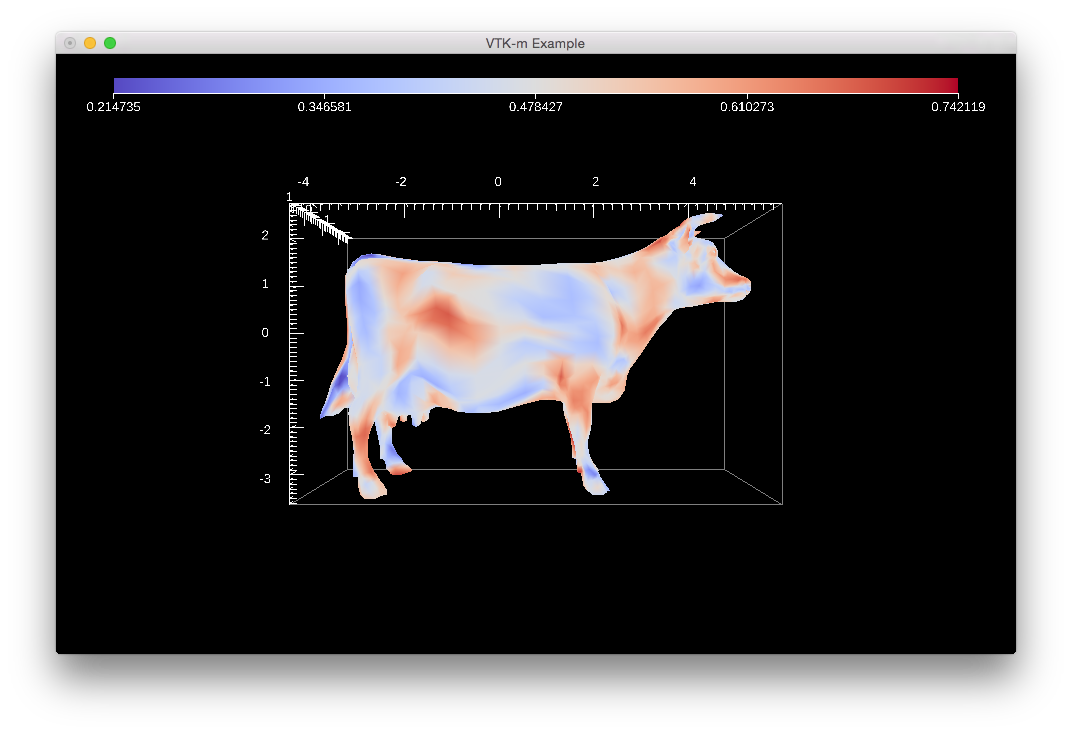
\includegraphics[width=4in]{images/BasicGlut}
  \caption{Output of the rendering program listed in
    Example~\ref{ex:BasicGlut}.}
  \label{fig:BasicGlut}
\end{figure}

\index{OpenGL|)}
\index{GLUT|)}
\index{canvas!OpenGL|)}
\index{canvas!GLUT|)}
\index{rendering!OpenGL|)}
\index{rendering!GLUT|)}

\subsection{Creating an Off Screen Rendering Canvas}

\index{rendering!off~screen|(}
\index{canvas!off~screen|(}
\index{off~screen|(}

Another use case for rendering in VTK-m is rendering to an off screen
buffer. This is the preferred method when doing automated visualization
such as when running visualization in situ with a simulation. VTK-m comes
built in with multiple methods to create off screen rendering contexts.
There are multiple subclasses to \vtkmrendering{Canvas} that, when
constructed, create their own rendering contexts, so can be used
immediately. All of these classes take as parameters to their constructors
the width and height of the image to create.

The following classes, when constructed, create an off screen rendering
buffer.

\begin{description}
\item[\vtkmrendering{CanvasOSMesa}] \index{rendering!OSMesa}
  \index{canvas!OSMesa} \index{OSMesa} Creates an off screen OpenGL
  rendering buffer using the OSMesa library. For this to be available,
  VTK-m must have been configured to use the OSMesa library. Also, be aware
  that OSMesa contexts do not use GPU hardware.
\item[\vtkmrendering{CanvasRayTracer}] \index{rendering!ray~tracing}
  \index{canvas!ray~tracing} \index{ray~tracing!canvas} Creates the frame
  buffers required for ray tracing. When invoking this canvas, you must use
  other ray tracing component where applicable. OpenGL rendering does not
  work with the \textidentifier{CanvasRayTracer}.
\end{description}

\index{canvas!off~screen!saving}
\index{off~screen!saving}

By their nature, when writing to an off screen canvas, you cannot directly
see the result. Typically, programs using off screen rendering save
rendered images as files to be viewed later. For convenience,
\textidentifier{Canvas} has a method named \textcode{SaveAs} that will
write the contents of the last saved image to a file. The files are written
in \index{portable~pixel~map}\index{PPM} portable pixel map (PPM) format,
which are also valid \index{portable~anymap~format}\index{PNM} portable
anymap format (PNM) files. This is a very simple format that is easy to
read and write. PPM files are supported by the
ImageMagick\footnote{\url{http://imagemagick.org}} software suite as well
as many other image software tools.

\vtkmlisting{Saving an image rendered in a \textidentifier{Canvas} to a file.}{SaveCanvasImage.cxx}

Alternately, the rendered image can be retrieved directly from the
\textidentifier{Canvas} by first calling the \textcode{RefreshColorBuffer}
method and then calling \textcode{GetColorBuffer}. This retrieves the raw
image data as a \vtkmcont{ArrayHandle}. \textidentifier{ArrayHandle}s are
documented later in Chapter~\ref{chap:ArrayHandle}.

\index{off~screen|)}
\index{canvas!off~screen|)}
\index{rendering!off~screen|)}

\index{canvas|)}
\index{rendering!canvas|)}


\section{Scenes and Actors}
\label{sec:Scene}
\label{sec:Actor}

\index{rendering!actor|(}
\index{actor|(}

The primary intent of the rendering package in VTK-m is to visually display
the data that is loaded and processed. Data are represented in VTK-m by
\vtkmcont{DataSet} objects. \textidentifier{DataSet} is presented in
Chapters \ref{chap:FileIO} and \ref{chap:ProvidedFilters}. For now we treat
\textidentifier{DataSet} mostly as an opaque object that can be passed
around readers, writers, filters, and rendering units. Detailed
documentation for \textidentifier{DataSet} is provided in
Chapter~\ref{chap:DataSet}.

To render a \textidentifier{DataSet}, the data are wrapped in a
\vtkmrendering{Actor} class. The \textidentifier{Actor} holds the
components of the \textidentifier{DataSet} to render (a cell set, a
coordinate system, and a field). A color table can also be optionally be
specified, but a default color table will be specified otherwise.

\index{actor|)}
\index{rendering!actor|)}

\index{rendering!scene|(}
\index{scene|(}

\textidentifier{Actor}s are collected together in an object called
\vtkmrendering{Scene}. An \textidentifier{Actor} is added to a
\textidentifier{Scene} with the \textcode{AddActor} method. The following
example demonstrates creating a \textidentifier{Scene} with one
\textidentifier{Actor}.

\index{scene|)}
\index{rendering!scene|)}

\vtkmlisting{Creating an \textidentifier{Actor} and adding it to a \textidentifier{Scene}.}{ActorScene.cxx}


\section{Mappers}
\label{sec:Mapper}

\index{rendering!mapper|(}
\index{mapper|(}

A \keyterm{mapper} is a unit that converts data (managed by an
\textidentifier{Actor}) and issues commands to the rendering subsystem to
generate images. All mappers in VTK-m are a subclass of
\vtkmrendering{Mapper}. Different rendering systems (as established by the
\textidentifier{Canvas}) often require different mappers. Also, different
mappers could render different types of data in different ways. For
example, one mapper might render polygonal surfaces whereas another might
render polyhedra as a translucent volume. Thus, a mapper should be picked
to match both the rendering system of the \textidentifier{Canvas} and the
data in the \textidentifier{Actor}.

The following mappers are provided by VTK-m.

\begin{description}
\item[\vtkmrendering{MapperGL}] Uses OpenGL to render surfaces. If the data
  contain polyhedra, then their faces are rendered.
  \textidentifier{MapperGL} only works in conjunction with
  \textidentifier{CanvasGL} or one of its subclasses.
\item[\vtkmrendering{MapperRayTracer}] Uses VTK-m's built in ray tracing
  system to render the visible surface of a mesh.
  \textidentifier{MapperRayTracer} only works in conjunction with
  \textidentifier{CanvasRayTracer}.
\item[\vtkmrendering{MapperVolume}] Uses VTK-m's built in ray tracing
  system to render polyhedra as a translucent volume.
  \textidentifier{MapperVolume} only works in conjunction with
  \textidentifier{CanvasRayTracer}.
\end{description}

\index{mapper|)}
\index{rendering!mapper|)}


\section{Views}

\index{rendering!view|(}
\index{view|(}

A \keyterm{view} is a unit that collects all the structures needed to
perform rendering. It contains everything needed to take a
\textidentifier{Scene} (Section~\ref{sec:Scene}) and use a
\textidentifier{Mapper} (Section~\ref{sec:Mapper}) to render it onto a
\textidentifier{Canvas} (Section~\ref{sec:Canvas}). The view also annotates
the image with spatial and scalar properties.

The base class for all views is \vtkmrendering{View}. \textidentifier{View}
is an abstract class, and you must choose one of the two provided
subclasses, \vtkmrendering{View3D} and \vtkmrendering{View2D}, depending on
the type of data being presented. (All three classes are defined in the
\vtkmheader{vtkm/rendering}{View.h} header file.) Both
\textidentifier{View3D} and \textidentifier{View2D} take a
\textidentifier{Scene}, a \textidentifier{Mapper}, and a
\textidentifier{Canvas} as arguments to their constructor.

\vtkmlisting[ex:ConstructView]{Constructing a \textidentifier{View}.}{ConstructView.cxx}

\index{color}
The \textidentifier{View} constructors also take an optional fourth
argument for the background color. The background color (like other colors)
is specified using the \vtkmrendering{Color} helper class, which manages
the red, green, and blue color channels as well as an optional alpha
channel. These channel values are given as floating point values between 0
and 1.

\vtkmlisting{Creating a \textidentifier{View} with a background color.}{ViewBackgroundColor.cxx}

Once the \textidentifier{View} is created but before it is used to render,
the \textcode{Initialize} method should be called. This is demonstrated in
Example~\ref{ex:ConstructView}.

Once the \textcode{Initialize} method is called, the \textidentifier{View}
is ready to render the scene. This happens by calling the \textcode{Paint}
method, which will render the data into the contained canvas. When using
GLUT, as in Example~\ref{ex:BasicGlut}, or with most other GUI-based
systems, \textcode{Paint} is called in the display callback.

\vtkmlisting{Using \textidentifier{Canvas}\textcode{::Paint} in a display callback.}{PaintView.cxx}

\index{view|)}
\index{rendering!view|)}


\section{Manipulating the Camera}

\index{rendering!camera|(}
\index{camera|(}

The \vtkmrendering{View} uses an object called \vtkmrendering{Camera} to
describe the vantage point from which to draw the geometry. The camera can
be retrieved from the \textidentifier{View}'s \textcode{GetCamera} method.
That retrieved camera can be directly manipulated or a new camera can be
provided by calling \textcode{SetCamera} on the \textidentifier{View}.

A \textidentifier{Camera} operates in one of two major modes: 2D mode or 3D
mode. 2D mode is designed for looking at flat geometry (or close to flat
geometry) that is parallel to the x-y plane. 3D mode provides the freedom
to place the camera anywhere in 3D space. The different modes can be set
with \textcode{SetModeTo2D} and \textcode{SetModeTo3D}, respectively. The
interaction with the camera in these two modes is very different.

\subsection{2D Camera Mode}

\index{rendering!camera!2D|(}
\index{camera!2D|(}

The 2D camera is restricted to looking at some region of the x-y plane.

\subsubsection{View Range}

\index{rendering!camera!view~range|(}
\index{camera!view~range|(}

The vantage point of a 2D camera can be specified by simply giving the
region in the x-y plane to look at. This region is specified by calling
\textcode{SetViewRange2D} on \textidentifier{Camera}. This method takes the
left, right, bottom, and top of the region to view. Typically these are set
to the range of the geometry in world space as shown in
Figure~\ref{fig:CameraViewRange2D}.

\begin{figure}[htb]
  \centering
  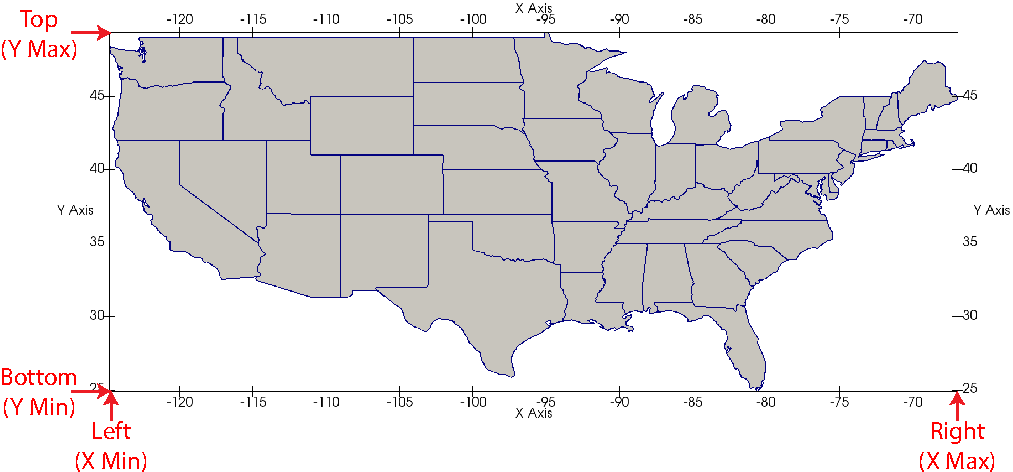
\includegraphics{images/CameraViewRange2D}
  \caption{The view range bounds to give a \textidentifier{Camera}.}
  \label{fig:CameraViewRange2D}
\end{figure}

There are 3 overloaded versions of the \textcode{SetViewRange2D} method.
The first version takes the 4 range values, left, right, bottom, and top,
as separate arguments in that order. The second version takes two
\vtkm{Range} objects specifying the range in the x and y directions,
respectively. The third version trakes a single \vtkm{Bounds} object, which
completely specifies the spatial range. (The range in z is ignored.) The
\textidentifier{Range} and \textidentifier{Bounds} objects are documented
later in Sections \ref{sec:Range} and \ref{sec:Bounds}, respectively.

\index{camera!view~range|)}
\index{rendering!camera!view~range|)}

\subsubsection{Pan}

\index{rendering!camera!pan|(}
\index{camera!pan|(}

A camera pan moves the viewpoint left, right, up, or down. A camera pan is
performed by calling the \textcode{Pan} method on \textidentifier{Camera}.
\textcode{Pan} takes two arguments: the amount to pan in x and the amount
to pan in y.

The pan is given with respect to the projected space. So a pan of $1$ in
the x direction moves the camera to focus on the right edge of the image
whereas a pan of $-1$ in the x direction moves the camera to focus on the
left edge of the image. When using \textcode{Pan} to respond to mouse
movements, a natural pan will divide the distance traveled by the mouse
pointer by the width and height of the screen as demonstrated in the
following example.

\vtkmlisting{Pan the view based on mouse movements.}{MousePan.cxx}

\index{camera!pan|)}
\index{rendering!camera!pan|)}

\subsubsection{Zoom}

\index{rendering!camera!zoom|(}
\index{camera!zoom|(}

A camera zoom draws the geometry larger or smaller. A camera zoom is
performed by calling the \textcode{Zoom} method on \textidentifier{Camera}.
\textcode{Zoom} takes a single argument specifying the zoom factor. A
positive number draws the geometry larger (zoom in), and larger zoom factor
results in larger geometry. Likewise, a negative number draws the geometry
smaller (zoom out). A zoom factor of 0 has no effect.

When using \textcode{Zoom} to respond to mouse movements, a natural zoom
will divide the distance traveled by the mouse pointer by the width or
height of the screen as demonstrated in the following example.

\vtkmlisting{Zoom the view based on mouse movements.}{MouseZoom.cxx}

\index{camera!zoom|)}
\index{rendering!camera!zoom|)}

\index{camera!2D|)}
\index{rendering!camera!2D|)}

\subsection{3D Camera Mode}

\index{rendering!camera!3D|(}
\index{camera!3D|(}

The 3D camera is a free-form camera that can be placed anywhere in 3D space
and can look in any direction. The projection of the 3D camera is based on
the \index{pinhole~camera}\index{camera!pinhole} pinhole camera model in
which all viewing rays intersect a single point. This single point is the
camera's position.

\subsubsection{Position and Orientation}

\index{rendering!camera!position}
\index{camera!position}
\index{rendering!camera!look~at}
\index{camera!look~at}
\index{look~at}
\index{rendering!camera!focal~point}
\index{camera!focal~point}
\index{focal~point}

The position of the camera, which is the point where the observer is
viewing the scene, can be set with the \textcode{SetPosition} method of
\textidentifier{Camera}. The direction the camera is facing is specified by
giving a position to focus on. This is called either the ``look at'' point
or the focal point and is specified with the \textcode{SetLookAt} method of
\textidentifier{Camera}. Figure~\ref{fig:CameraPositionOrientation3D} shows
the relationship between the position and look at points.

\begin{figure}[htb]
  \centering
  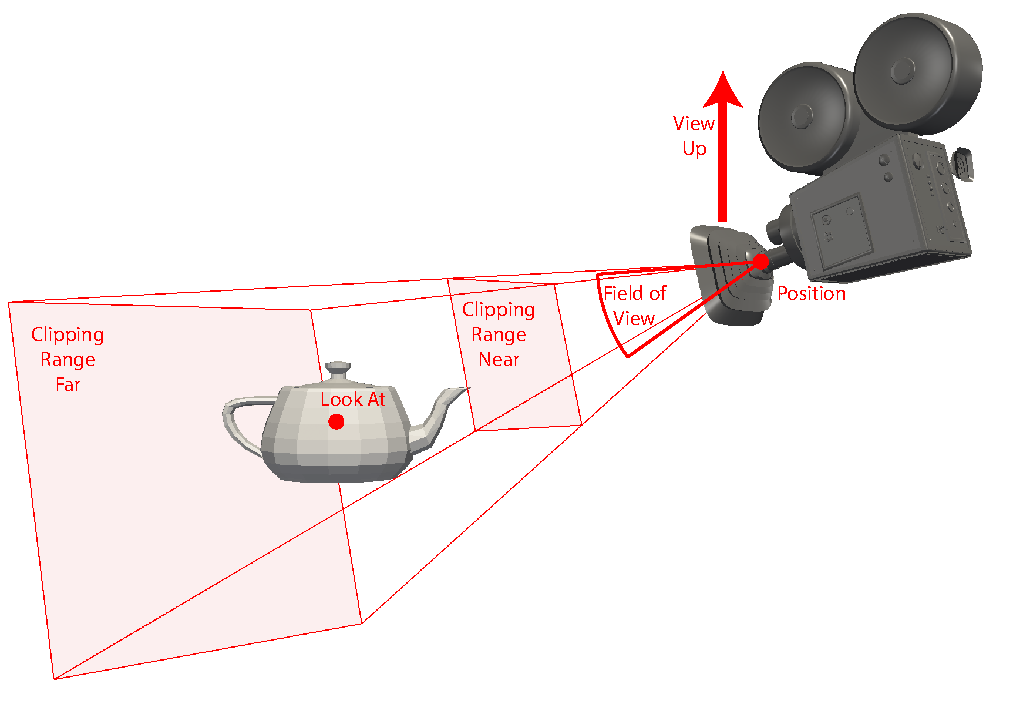
\includegraphics{images/CameraPositionOrientation}
  \caption{The position and orientation parameters for a
    \textidentifier{Camera}.}
  \label{fig:CameraPositionOrientation3D}
\end{figure}

\index{rendering!camera!view~up}
\index{rendering!camera!up}
\index{camera!view~up}
\index{camera!up}
\index{view~up}

In addition to specifying the direction to point the camera, the camera
must also know which direction is considered ``up.'' This is specified with
the view up vector using the \textcode{SetViewUp} method in
\textidentifier{Camera}. The view up vector points from the camera position
(in the center of the image) to the top of the image. The view up vector in
relation to the camera position and orientation is shown in
Figure~\ref{fig:CameraPositionOrientation3D}.

\index{rendering!camera!field~of~view}
\index{camera!field~of~view}
\index{field~of~view}

Another important parameter for the camera is its field of view. The field
of view specifies how wide of a region the camera can see. It is specified
by giving the angle in degrees of the cone of visible region emanating from
the pinhole of the camera to the \textcode{SetFieldOfView} method in the
\textidentifier{Camera}. The field of view angle in relation to the camera
orientation is shown in Figure~\ref{fig:CameraPositionOrientation3D}. A
field of view angle of $60^{\circ}$ usually works well.

\index{rendering!camera!clipping~range}
\index{camera!clipping~range}
\index{clipping~range}
\index{rendering!camera!near~clip~plane}
\index{camera!near~clip~plane}
\index{near~clip~plane}
\index{rendering!camera!far~clip~plane}
\index{camera!far~clip~plane}
\index{far~clip~plane}

Finally, the camera must specify a clipping region that defines the valid
range of depths for the object. This is a pair of planes parallel to the
image that all visible data must lie in. Each of these planes is defined
simply by their distance to the camera position. The near clip plane is
closer to the camera and must be in front of all geometry. The far clip
plane is further from the camera and must be behind all geometry. The
distance to both the near and far planes are specified with the
\textcode{SetClippingRange} method in \textidentifier{Camera}.
Figure~\ref{fig:CameraPositionOrientation3D} shows the clipping planes in
relationship to the camera position and orientation.

\vtkmlisting{Directly setting \protect\vtkmrendering{Camera} position and orientation.}{CameraPositionOrientation.cxx}

\subsubsection{Movement}

In addition to specifically setting the position and orientation of the
camera, \vtkmrendering{Camera} contains several convenience methods that
move the camera relative to its position and look at point.

\index{rendering!camera!elevation}
\index{camera!elevation}
\index{elevation}

\index{rendering!camera!azimuth}
\index{camera!azimuth}
\index{azimuth}

Two such methods are elevation and azimuth, which move the camera around
the sphere centered at the look at point. \textcode{Elevation} raises or
lowers the camera. Positive values raise the camera up (in the direction of
the view up vector) whereas negative values lower the camera down.
\textcode{Azimuth} moves the camera around the look at point to the left or
right. Positive values move the camera to the right whereas negative values
move the camera to the left. Both \textcode{Elevation} and
\textcode{Azimuth} specify the amount of rotation in terms of degrees.
Figure~\ref{fig:CameraMovement} shows the relative movements of
\textcode{Elevation} and \textcode{Azimuth}.

\begin{figure}[htb]
  \centering
  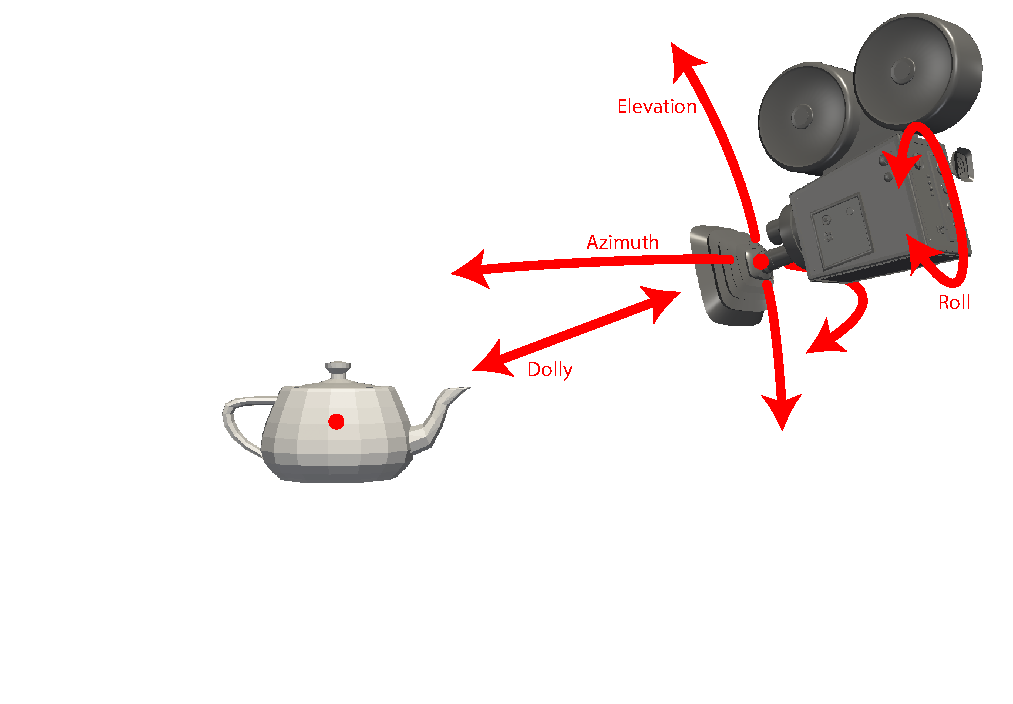
\includegraphics{images/CameraMovement}
  \caption{\textidentifier{Camera} movement functions relative to position
    and orientation.}
  \label{fig:CameraMovement}
\end{figure}

\vtkmlisting{Moving the camera around the look at point.}{CameraMovement.cxx}

\begin{commonerrors}
  The \textcode{Elevation} and \textcode{Azimuth} methods change the
  position of the camera, but not the view up vector. This can cause some
  wild camera orientation changes when the direction of the camera view is
  near parallel to the view up vector, which often happens when the
  elevation is raised or lowered by about 90 degrees.
\end{commonerrors}

In addition to rotating the camera around the look at point, you can move
the camera closer or further from the look at point. This is done with the
\textcode{Dolly} method. The \textcode{Dolly} method takes a single value
that is the factor to scale the distance between camera and look at point.
Values greater than one move the camera away, values less than one move the
camera closer. The direction of dolly movement is shown in
Figure~\ref{fig:CameraMovement}.

Finally, the \textcode{Roll} method rotates the camera around the viewing
direction. It has the effect of rotating the rendered image. The
\textcode{Roll} method takes a single value that is the angle to rotate in
degrees. The direction of roll movement is shown in
Figure~\ref{fig:CameraMovement}.

\subsubsection{Interactive Rotations}

\index{rendering!camera!mouse|(}
\index{camera!mouse|(}
\index{mouse~rotation|(}

A common and important mode of interaction with 3D views is to allow the
user to rotate the object under inspection by dragging the mouse. To
facilitate this type of interactive rotation, \vtkmrendering{Camera}
provides a convenience method named \textcode{TrackballRotate}. The
\textcode{TrackballRotate} method takes a start and end position of the
mouse on the image and rotates viewpoint as if the user grabbed a point on
a sphere centered in the image at the start position and moved under the
end position.

The \textcode{TrackballRotate} method is typically called from within a
mouse movement callback. The callback must record the pixel position from
the last event and the new pixel position of the mouse. Those pixel
positions must be normalized to the range -1 to 1 where the position
(-1,-1) refers to the lower left of the image and (1,1) refers to the upper
right of the image. The following example demonstrates the typical
operations used to establish rotations when dragging the mouse.

\vtkmlisting{Interactive rotations through mouse dragging with \textidentifier{Camera}\textcode{::TrackballRotate}.}{MouseRotate.cxx}

\index{mouse~rotation|)}
\index{camera!mouse|)}
\index{rendering!camera!mouse|)}

\subsubsection{Pan}

\index{rendering!camera!pan|(}
\index{camera!pan|(}

A camera pan moves the viewpoint left, right, up, or down. A camera pan is
performed by calling the \textcode{Pan} method on \textidentifier{Camera}.
\textcode{Pan} takes two arguments: the amount to pan in x and the amount
to pan in y.

The pan is given with respect to the projected space. So a pan of $1$ in
the x direction moves the camera to focus on the right edge of the image
whereas a pan of $-1$ in the x direction moves the camera to focus on the
left edge of the image. When using \textcode{Pan} to respond to mouse
movements, a natural pan will divide the distance traveled by the mouse
pointer by the width and height of the screen as demonstrated in the
following example.

\vtkmlisting{Pan the view based on mouse movements.}{MousePan.cxx}

\textcode{Pan} operates in image space, not world space. Panning does not
change the camera position or orientation. Thus the look at point will be
off center with respect to the image.

\index{camera!pan|)}
\index{rendering!camera!pan|)}

\subsubsection{Zoom}

\index{rendering!camera!zoom|(}
\index{camera!zoom|(}

A camera zoom draws the geometry larger or smaller. A camera zoom is
performed by calling the \textcode{Zoom} method on \textidentifier{Camera}.
\textcode{Zoom} takes a single argument specifying the zoom factor. A
positive number draws the geometry larger (zoom in), and larger zoom factor
results in larger geometry. Likewise, a negative number draws the geometry
smaller (zoom out). A zoom factor of 0 has no effect.

When using \textcode{Zoom} to respond to mouse movements, a natural zoom
will divide the distance traveled by the mouse pointer by the width or
height of the screen as demonstrated in the following example.

\vtkmlisting{Zoom the view based on mouse movements.}{MouseZoom.cxx}

\textcode{Zoom} operates in image space, not world space. Zooming differs
from \textcode{Dolly} in that the reported position of the camera does not
change. Instead, the image gets magnified or shrunk.

\index{camera!zoom|)}
\index{rendering!camera!zoom|)}

\index{camera!3D|)}
\index{rendering!camera!3D|)}

\index{camera|)}
\index{rendering!camera|)}

\index{rendering|)}

\subsubsection{Reset}

\index{rendering!camera!reset|(}
\index{camera!reset|(}

\fix{ResetToBounds}
\fix{Add example to reset down axis}
\fix{Also available for 2D cameras}

\vtkmlisting{Resetting a \textidentifier{Camera} to view geometry.}{ResetCamera.cxx}

\vtkmlisting{Resetting a \textidentifier{Camera} to be axis aligned.}{AxisAlignedCamera.cxx}

\index{camera!reset|)}
\index{rendering!camera!reset|)}


\section{Color Tables}
\label{sec:ColorTables}

\index{rendering!color~tables|(}
\index{color~tables|(}

\index{color~tables|)}
\index{rendering!color~tables|)}


}{}

\ifthenelse{\equal{\buildtype}{Full} \OR \equal{\buildtype}{Using}}{

  \part{Using VTK-m}
  \label{part:Using}

  % -*- latex -*-

\chapter{Basic Provisions}
\label{chap:BasicProvisions}

This section describes the core facilities provided by VTK-m. These include
macros, types, and classes that define the environment in which code is
run, the core types of data stored, and template introspection. We also
start with a description of package structure used by VTK-m.


\section{General Approach}
\label{sec:GeneralApproach}

VTK-m is designed to provide a \keyterm{pervasive parallelism}
\index{pervasive parallelism} throughout all its visualization algorithms,
meaning that the algorithm is designed to operate with independent
concurrency at the finest possible level throughout. VTK-m provides this
pervasive parallelism by providing a programming construct called a
\keyterm{worklet}, \index{worklet} which operates on a very fine
granularity of data. The worklets are designed as serial components, and
VTK-m handles whatever layers of concurrency are necessary, thereby
removing the onus from the visualization algorithm developer. Worklet
operation is then wrapped into \keyterm{filters}, \index{filter} which
provide a simplified interface to end users.

A worklet is essentially a small functor \index{functor} or kernel
\index{kernel} designed to operate on a small element of data. (The name
``worklet'' means a small amount of work. We mean small in this sense to be
the amount of data, not necessarily the amount of instructions performed.)
The worklet is constrained to contain a serial and stateless function.
These constraints form three critical purposes. First, the constraints on
the worklets allow VTK-m to schedule worklet invocations on a great many
independent concurrent threads and thereby making the algorithm pervasively
parallel. Second, the constraints allow VTK-m to provide thread safety. By
controlling the memory access the toolkit can insure that no worklet will
have any memory collisions, false sharing, or other parallel programming
pitfalls. Third, the constraints encourage good programming practices. The
worklet model provides a natural approach to visualization algorithm design
that also has good general performance characteristics.

VTK-m allows developers to design algorithms that are run on massive
amounts of threads. However, VTK-m also allows developers to interface to
applications, define data, and invoke algorithms that they have written or
are provided otherwise. These two modes represent significantly different
operations on the data. The operating code of an algorithm in a worklet is
constrained to access only a small portion of data that is provided by the
framework. Conversely, code that is building the data structures needs to
manage the data in its entirety, but has little reason to perform
computations on any particular element.

Consequently, VTK-m is divided into two \keyterm{environments}
\index{environment} that handle each of these use cases. Each environment
has its own API, and direct interaction between the environments is
disallowed. The environments are as follows.

\begin{description}
\item[Execution Environment] \index{execution environment}
  \index{environment!execution} This is the environment in which the
  computational portion of algorithms are executed. The API for this
  environment provides work for one element with convenient access to
  information such as connectivity and neighborhood as needed by typical
  visualization algorithms. Code for the execution environment is designed
  to always execute on a very large number of threads.
\item[Control Environment] \index{control environment}
  \index{environment!control} This is the environment that is used to
  interface with applications, interface with I/O devices, and schedule
  parallel execution of the algorithms. The associated API is designed for
  users that want to use VTK-m to analyze their data using provided or
  supplied filters. Code for the control environment is designed to run on
  a single thread (or one single thread per process in an MPI job).
\end{description}

These dual programming environments are partially a convenience to isolate
the application from the execution of the worklets and are partially a
necessity to support GPU languages with host and device environments. The
control and execution environments are logically equivalent to the host and
device environments, respectively, in CUDA and other associated GPU
languages.

\begin{figure}[htb]
  \centering
  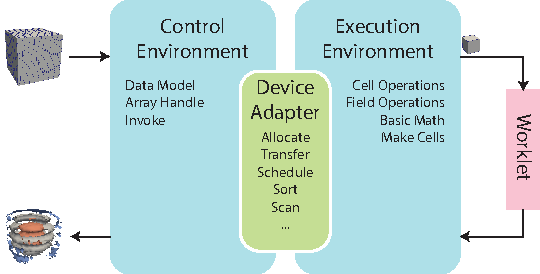
\includegraphics[width=4in]{images/VTKmEnvironments}
  \caption{Diagram of the VTK-m framework.}
  \label{fig:VTKmDiagram}
\end{figure}

Figure~\ref{fig:VTKmDiagram} displays the relationship between the control
and execution environment. The typical workflow when using VTK-m is that
first the control thread establishes a data set in the control environment
and then invokes a parallel operation on the data using a filter. From
there the data is logically divided into its constituent elements, which
are sent to independent invocations of a worklet. The worklet
invocations, being independent, are run on as many concurrent threads as
are supported by the device. On completion the results of the worklet
invocations are collected to a single data structure and a handle is
returned back to the control environment.

\begin{didyouknow}
  Are you only planning to use filters in VTK-m that already exist? If so,
  then everything you work with will be in the control environment. The
  execution environment is only used when implementing algorithms for
  filters.
\end{didyouknow}


\section{Package Structure}
\label{sec:PackageStructure}

\index{packages|(}

VTK-m is organized in a hierarchy of nested packages. VTK-m places
definitions in \keyterm{namespaces} \index{namespace} that correspond to
the package (with the exception that one package may specialize a template
defined in a different namespace).

The base package is named \vtkm{}. All classes within VTK-m are placed
either directly in the \vtkm{} package or in a package beneath it. This
helps prevent name collisions between VTK-m and any other library.

As described in Section~\ref{sec:GeneralApproach}, the VTK-m API is divided
into two distinct environments: \index{environment} the control environment
\index{control environment} \index{environment!control} and the execution
environment. \index{execution environment} \index{environment!execution}
The API for these two environments are located in the \vtkmcont{} and
\vtkmexec{} packages, respectively. Items located in the base \vtkm{}
namespace are available in both environments.

Although it is conventional to spell out names in identifiers (see the
coding conventions in Chapter~\ref{chap:CodingConventions}), there is an
exception to abbreviate control and execution to \textnamespace{cont}
and \textnamespace{exec}, respectively. This is because it is also part of
the coding convention to declare the entire namespace when using an
identifier that is part of the corresponding package. The shorter names
make the identifiers easier to read, faster to type, and more feasible to
pack lines in 80 column displays. These abbreviations are also used instead
of more common abbreviations (e.g. ctrl for control) because, as part of
actual English words, they are easier to type.

Further functionality in VTK-m is built on top of the base \vtkm{},
\vtkmcont{}, and \vtkmexec{} packages. Support classes for building
worklets, described in Chapter~\ref{chap:Worklets}, are contained in the
\vtkmworklet{} package. Other facilities in VTK-m are provided in their own
packages such as \vtkmio{}, \vtkmfilter{}, and \vtkmrendering{}. These
packages are described in Part~\ref{part:GettingStarted}.

VTK-m contains code that uses specialized compiler features, such as those
with CUDA, or libraries, such as Intel Threading Building Blocks, that will
not be available on all machines. Code for these features are encapsulated
in their own packages under the \vtkmcont{} namespace: \vtkmcontcuda{} and
\vtkmconttbb{}.

VTK-m contains OpenGL interoperability \index{OpenGL}
\index{interoperability} that allows data generated with VTK-m to be
efficiently transferred to OpenGL objects. This feature is encapsulated in
the \vtkmopengl{} package.

Figure~\ref{fig:Packages} provides a diagram of the VTK-m package hierarchy.

\begin{figure}[htb]
  \centering
  %% \begin{itemize}
  %% \item \vtkm{}
  %% \item \vtkmexec{}
  %% \item \vtkmcont{}
  %% \item \vtkmcontcuda{}
  %% \item \vtkmconttbb{}
  %% \item \vtkmio{}
  %% \item \vtkmioreader{}
  %% \item \vtkmiowriter{}
  %% \item \vtkmfilter{}
  %% \item \vtkmrendering{}
  %% \item \vtkmopengl{}
  %% \item \vtkmworklet{}
  %% %% \item \textnamespace{vtkm}
  %% %%   \begin{itemize}
  %% %%   \item \textnamespace{cont}
  %% %%   \item \textnamespace{exec}
  %% %%   \item \textnamespace{worklet}
  %% %%   \item \textnamespace{math}
  %% %%   \item \textnamespace{cuda}
  %% %%     \begin{itemize}
  %% %%     \item \textnamespace{cont}
  %% %%     \end{itemize}
  %% %%   \item \textnamespace{openmp}
  %% %%     \begin{itemize}
  %% %%     \item \textnamespace{cont}
  %% %%     \end{itemize}
  %% %%   \item \textnamespace{tbb}
  %% %%     \begin{itemize}
  %% %%     \item \textnamespace{cont}
  %% %%     \end{itemize}
  %% %%   \item \textnamespace{opengl}
  %% %%   \end{itemize}
  %% \end{itemize}
  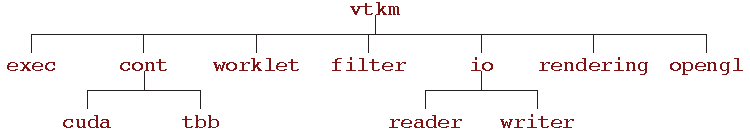
\includegraphics{images/PackageHierarchy}
  \caption{VTK-m package hierarchy.}
  \label{fig:Packages}
\end{figure}

By convention all classes will be defined in a file with the same name as
the class name (with a \textfilename{.h} extension) located in a directory
corresponding to the package name. For example, the \vtkmcont{ArrayHandle}
class is found in the \vtkmheader{vtkm/cont}{ArrayHandle.h} header. There
are, however, exceptions to this rule. Some smaller classes and types are
grouped together for convenience. These exceptions will be noted as
necessary.

Within each namespace there may also
be \textnamespace{internal}\indexnamespaceone{internal}
and \textnamespace{detail}\indexnamespaceone{detail}
sub-namespaces. The \textnamespace{internal} namespaces contain features
that are used internally and may change without
notice. The \textnamespace{detail} namespaces contain features that are
used by a particular class but must be declared outside of that
class. Users should generally ignore classes in these namespaces.

\index{packages|)}


\section{Function and Method Environment Modifiers}
\label{sec:FunctionAndMethodEnvironmentModifiers}

Any function or method defined by VTK-m must come with a modifier that determines in which environments the function may be run.
These modifiers are C macros that VTK-m uses to instruct the compiler for which architectures to compile each method.
Most user code outside of VTK-m need not use these macros with the important exception of any classes passed to VTK-m.
This occurs when defining new worklets, array storage, and device adapters.

VTK-m provides three modifier macros, \vtkmcontmodifier, \vtkmexecmodifier, and
\vtkmexeccontmodifier, which are used to declare functions and methods that
can run in the control environment, execution environment, and both
environments, respectively. These macros get defined by including just
about any VTK-m header file, but including \vtkmheader{vtkm}{Types.h} will
ensure they are defined. 

The modifier macro is placed after the template declaration, if there is one,
and before the return type for the function. Here is a simple example of a
function that will square a value. Since most types you would use this
function on have operators in both the control and execution environments,
the function is declared for both places.

\vtkmlisting{Usage of an environment modifier macro on a function.}{EnvironmentModifierMacro.cxx}

The primary function of the modifier macros is to inject compiler-specific
keywords that specify what architecture to compile code for. For example,
when compiling with CUDA\index{CUDA}, the control modifiers have
\textcode{\_\_host\_\_}\index{\_\_host\_\_} in them and execution modifiers
have \textcode{\_\_device\_\_}\index{\_\_device\_\_} in them.

There is one additional modifier macro that is not used for functions but
rather used when declaring a constant data object that is used in the
execution environment. This macro is named
\vtkmmacro{VTKM\_EXEC\_CONSTANT}\index{modifier!constant}\index{constant modifier}
and is used to declare a constant lookup table used when executing a
worklet. Its primary reason for existing is to add a
\textcode{\_\_constant\_\_} keyword when compiling with CUDA. This modifier
currently has no effect on any other compiler.

Finally, it is sometimes the case that a function declared as
\vtkmexeccontmodifier has to call a method declared as \vtkmexecmodifier or
\vtkmcontmodifier. Generally functions should not call other functions with
incompatible control/execution modifiers, but sometimes a generic
\vtkmexeccontmodifier function calls another function determined by the
template parameters, and the valid environments of this subfunction may be
inconsistent. For cases like this, you can use the
\vtkmmacro{VTKM\_SUPPRESS\_EXEC\_WARNINGS} to tell the compiler to ignore the
inconsistency when resolving the template. When applied to a templated
function or method, \vtkmmacro{VTKM\_SUPPRESS\_EXEC\_WARNINGS} is placed
before the \textcode{template} keyword. When applied to a non-templated
method in a templated class, \vtkmmacro{VTKM\_SUPPRESS\_EXEC\_WARNINGS} is
placed before the environment modifier macro.

\vtkmlisting{Suppressing warnings about functions from mixed environments.}{SuppressExecWarnings.cxx}


\section{Core Data Types}
\label{sec:CoreDataTypes}

Except in rare circumstances where precision is not a concern, VTK-m does
not directly use the core C types like \textcode{int}, \textcode{float},
and \textcode{double}. Instead, VTK-m provides its own core types, which
are declared in \vtkmheader{vtkm}{Types.h}.

\subsection{Single Number Types}

To ensure portability across different compilers and architectures, VTK-m
provides \textcode{typedef}s for the following basic types with explicit
precision: \vtkm{Float32}, \vtkm{Float64}, \vtkm{Int8}, \vtkm{Int16},
\vtkm{Int32}, \vtkm{Int64}, \vtkm{UInt8}, \vtkm{UInt16}, \vtkm{UInt32}, and
\vtkm{UInt64}. Under most circumstances when using VTK-m (and performing
visualization in general) the type of data is determined by the source of the
data or resolved through templates. In the case where a specific type of
data is required, these VTK-m--defined types should be preferred over basic
C types like \textcode{int} or \textcode{float}.

Many of the structures in VTK-m require indices to identify elements like
points and cells. All indices for arrays and other lists use the type
\vtkm{Id}. By default this type is a 32-bit wide integer but can be easily
changed by compile options. The CMake configuration option
\cmakevar{VTKM\_USE\_64BIT\_IDS} can be used to change \vtkm{Id} to be 64
bits wide. This configuration can be overridden by defining the C macro
\vtkmmacro{VTKM\_USE\_64BIT\_IDS} or \vtkmmacro{VTKM\_NO\_64BIT\_IDS} to
force \vtkm{Id} to be either 64 or 32 bits. These macros must be defined
before any VTK-m header files are included to take effect.

There is also a secondary index type named \vtkm{IdComponent} that is used
to index components of short vectors (discussed in
Section~\ref{sec:VectorTypes}). This type is an integer that might be a
shorter width than \vtkm{Id}.

There is also the rare circumstance in which an algorithm in VTK-m computes
data values for which there is no indication what the precision should
be. For these circumstances, the type \vtkm{FloatDefault} is provided. By
default this type is a 32-bit wide floating point number but can be easily
changed by compile options. The CMake configuration option
\cmakevar{VTKM\_USE\_DOUBLE\_PRECISION} can be used to change
\vtkm{FloatDefault} to be 64 bits wide. This configuration can be
overridden by defining the C macro \vtkmmacro{VTKM\_USE\_DOUBLE\_PRECISION}
or \vtkmmacro{VTKM\_NO\_DOUBLE\_PRECISION} to force \vtkm{FloatDefault} to
be either 64 or 32 bits. These macros must be defined before any VTK-m
header files are included to take
effect.

For convenience, you can include either
\vtkmheader{vtkm/internal}{ConfigureFor32.h} or
\vtkmheader{vtkm/internal}{ConfigureFor64.h} to force both \vtkm{Id} and
\vtkm{FloatDefault} to be 32 or 64 bits.

\subsection{Vector Types}
\label{sec:VectorTypes}

Visualization algorithms also often require operations on short vectors.
Arrays indexed in up to three dimensions are common. Data are often defined
in 2-space and 3-space, and transformations are typically done in
homogeneous coordinates of length 4. To simplify these types of operations,
VTK-m provides the \vtkm{Vec}\tparams{T,Size} templated type, which is
essentially a fixed length array of a given type.

The default constructor of \vtkm{Vec} objects leaves the values
uninitialized. All vectors have a constructor with one argument that is
used to initialize all components. All \vtkm{Vec} objects with a size of 4
or less is specialized to also have a constructor that allows you to set
the individual components. Likewise, there is a \vtkm{make\_Vec} function
that builds initialized vector types of up to 4 components. Once created,
you can use the bracket operator to get and set component values with the
same syntax as an array.

\vtkmlisting{Creating vector types.}{CreatingVectorTypes.cxx}

The types \vtkm{Id2} and \vtkm{Id3} are \textcode{typedef}s of
\vtkm{Vec}\tparams{\vtkm{Id},2} and \vtkm{Vec}\tparams{\vtkm{Id},2}. These
are used to index arrays of 2 and 3 dimensions, which is common.

Vectors longer than 4 are also supported, but independent component values must be set after construction.
The \vtkm{Vec} class contains a constant named \textidentifier{NUM\_COMPONENTS}\index{NUM\_COMPONENTS} to specify how many components are in the vector.
The class also has a \textcode{GetNumberOfComponents} method that also returns the number of components that are in the vector.

\vtkmlisting{A Longer Vector.}{LongerVector.cxx}

\vtkm{Vec} supports component-wise arithmetic using the operators
for plus (\textcode{+}), minus (\textcode{-}), multiply (\textcode{*}), and
divide (\textcode{/}). It also supports scalar to vector multiplication
with the multiply operator. The comparison operators equal (\textcode{==})
is true if every pair of corresponding components are true and not equal
(\textcode{!=}) is true otherwise. A special \vtkm{dot} function is
overloaded to provide a dot product for every type of vector.

\vtkmlisting{Vector operations.}{VectorOperations.cxx}

These operators, of course, only work if they are also defined for the
component type of the \vtkm{Vec}. For example, the multiply operator will
work fine on objects of type \vtkm{Vec}\tparams{char,3}, but the multiply
operator will not work on objects of type \vtkm{Vec}\tparams{std::string,3}
because you cannot multiply objects of type \textcode{std::string}.

In addition to generalizing vector operations and making arbitrarily long
vectors, \vtkm{Vec} can be repurposed for creating any sequence of
homogeneous objects. Here is a simple example of using \vtkm{Vec} to hold
the state of a polygon.

\vtkmlisting{Repurposing a \protect\vtkm{Vec}.}{EquilateralTriangle.cxx}

\index{Vec-like|(}

The \vtkm{Vec} class provides a convenient structure for holding and passing small vectors of data.
However, there are times when using \textidentifier{Vec} is inconvenient or inappropriate.
For example, the size of \vtkm{Vec} must be known at compile time, but there may be need for a vector whose size is unknown until compile time.
Also, the data populating a \vtkm{Vec} might come from a source that makes it inconvenient or less efficient to construct a \vtkm{Vec}.
For this reason, \VTKm also provides several \keyterm{\Veclike} objects that behave much like \vtkm{Vec} but are a different class.
These \Veclike objects have the same interface as \vtkm{Vec} except that the \textidentifier{NUM\_COMPONENTS} constant is not available on those that are sized at run time.
\Veclike objects also come with a \textcode{CopyInto} method that will take their contents and copy them into a standard \textidentifier{Vec} class.
(The standard \textidentifier{Vec} class also has a \textcode{CopyInto} method for consistency.)

The first \Veclike object is \vtkm{VecC}, which exposes a C-type array as a \textidentifier{Vec}.
The constructor for \vtkm{VecC} takes a C array and a size of that array.
There is also a constant version of \textidentifier{VecC} named \vtkm{VecCConst}, which takes a constant array and cannot be mutated.
The \vtkmheader{vtkm}{Types.h} header defines both \textidentifier{VecC} and \textidentifier{VecCConst} as well as multiple versions of \vtkm{make\_VecC} to easily convert a C array to either a \textidentifier{VecC} or \textidentifier{VecCConst}.

The following example demonstrates converting values from a constant table into a \vtkm{VecCConst} for further consumption.
The table and associated methods define how 8 points come together to form a hexahedron.

\vtkmlisting[ex:VecCConst]{Using \protect\vtkm{VecCConst} with a constant array.}{VecCExample.cxx}

\begin{commonerrors}
  The \vtkm{VecC} and \vtkm{VecCConst} classes only hold a pointer to a buffer that contains the data.
  They do not manage the memory holding the data.
  Thus, if the pointer given to \vtkm{VecC} or \vtkm{VecCConst} becomes invalid, then using the object becomes invalid.
  Make sure that the scope of the \vtkm{VecC} or \vtkm{VecCConst} does not outlive the scope of the data it points to.
\end{commonerrors}

The next \Veclike object is \vtkm{VecVariable}, which provides a \Veclike object that can be resized at run time to a maximum value.
Unlike \textidentifier{VecC}, \textidentifier{VecVariable} holds its own memory, which makes it a bit safer to use.
But also unlike \textidentifier{VecC}, you must define the maximum size of \textidentifier{VecVariable} at compile time.
Thus, \textidentifier{VecVariable} is really only appropriate to use when there is a predetermined limit to the vector size that is fairly small.

The following example uses a \vtkm{VecVariable} to store the trace of edges within a hexahedron.
This example uses the methods defined in Example~\ref{ex:VecCConst}.

\vtkmlisting{Using \protect\vtkm{VecVariable}.}{VecVariableExample.cxx}

\VTKm provides further examples of \Veclike objects as well.
For example, the \vtkm{VecFromPortal} and \vtkm{VecFromPortalPermute} objects allow you to treat a subsection of an arbitrarily large array as a \textidentifier{Vec}.
These objects work by attaching to array portals, which are described in Section~\ref{sec:ArrayPortals}.
Another example of a \Veclike object is \vtkm{VecRectilinearPointCoordinates}, which efficiently represents the point coordinates in an axis-aligned hexahedron.
Such shapes are common in structured grids.
These and other data sets are described in Chapter~\ref{chap:DataSets}.

\index{Vec-like|)}


\subsection{Pair}
\label{sec:Pair}

VTK-m defines a \vtkm{Pair}\tparams{T1,T2} templated object that
behaves just like \textcode{std:\colonhyp{}pair} from the standard template
library. The difference is that \vtkm{Pair} will work in both the execution
and control environment, whereas the STL \textcode{std::pair} does not
always work in the execution environment.

The VTK-m version of \vtkm{Pair} supports the same types, fields, and
operations as the STL version. VTK-m also provides a \vtkm{make\_Pair}
function for convenience.

\subsection{Range}
\label{sec:Range}

VTK-m provides a convenience structure named \vtkm{Range} to help manage a
range of values. The \textidentifier{Range} \textcode{struct} contains two
data members, \textcode{Min} and \textcode{Max}, which represent the ends
of the range of numbers. \textcode{Min} and \textcode{Max} are both of type
\vtkm{Float64}. \textcode{Min} and \textcode{Max} can be directly accessed,
but \textidentifier{Range} also comes with the following helper functions
to make it easier to build and use ranges. Note that all of these functions
treat the minimum and maximum value as inclusive to the range.

\begin{description}
\item[\textcode{IsNonEmpty}] Returns true if the range covers at least one
  value.
\item[\textcode{Contains}] Takes a single number and returns true if that
  number is contained within the range.
\item[\textcode{Length}] Returns the distance between \textcode{Min} and
  \textcode{Max}. Empty ranges return a length of 0. Note that if the range
  is non-empty and the length is 0, then \textcode{Min} and \text{Max} must
  be equal, and the range contains exactly one number.
\item[\textcode{Center}] Returns the number equidistant to \textcode{Min}
  and \textcode{Max}. If the range is empty, NaN is returned.
\item[\textcode{Include}] Takes either a single number or another range and
  modifies this range to include the given number or range. If necessary,
  the range is grown just enough to encompass the given argument. If the
  argument is already in the range, nothing changes.
\item[\textcode{Union}] A nondestructive version of \textcode{Include},
  which builds a new \textidentifier{Range} that is the union of this range
  and the argument. The \textcode{+} operator is also overloaded to compute
  the union.
\end{description}

The following example demonstrates the operation of \vtkm{Range}.

\vtkmlisting{Using \protect\vtkm{Range}.}{UsingRange.cxx}

\subsection{Bounds}
\label{sec:Bounds}

VTK-m provides a convenience structure named \vtkm{Bounds} to help manage
an axis-aligned region in 3D space. Among other things, this structure is
often useful for representing a bounding box for geometry. The
\textidentifier{Bounds} \textcode{struct} contains three data members,
\textcode{X}, \textcode{Y}, and \textcode{Z}, which represent the range of
the bounds along each respective axis. All three of these members are of
type \vtkm{Range}, which is discussed previously in
Section~\ref{sec:Range}. \textcode{X}, \textcode{Y}, and \textcode{Z} can
be directly accessed, but \textidentifier{Bounds} also comes with the
following helper functions to make it easier to build and use ranges.

\begin{description}
\item[\textcode{IsNonEmpty}] Returns true if the bounds cover at least one
  value.
\item[\textcode{Contains}] Takes a \vtkm{Vec} of size 3 and returns true if
  those point coordinates are contained within the range.
\item[\textcode{Center}] Returns the point at the center of the range as a
  \vtkm{Vec}\textcode{<}\vtkm{Float64}\textcode{,3>}.
\item[\textcode{Include}] Takes either a \vtkm{Vec} of size 3 or another
  bounds and modifies this bounds to include the given point or bounds. If
  necessary, the bounds are grown just enough to encompass the given
  argument. If the argument is already in the bounds, nothing changes.
\item[\textcode{Union}] A nondestructive version of \textcode{Include},
  which builds a new \textidentifier{Bounds} that is the union of this
  bounds and the argument. The \textcode{+} operator is also overloaded to
  compute the union.
\end{description}

The following example demonstrates the operation of \vtkm{Bounds}.

\vtkmlisting{Using \protect\vtkm{Bounds}.}{UsingBounds.cxx}


\section{Traits}
\label{sec:Traits}

\index{traits|(}

When using templated types, it is often necessary to get information about
the type or specialize code based on general properties of the type. VTK-m
uses traits classes to publish and retrieve information about types. A
traits class is simply a templated structure that provides typedefs for
tag\index{tag} structures, empty types used for identification. The traits
classes might also contain constant numbers and helpful static
functions. See {\it Effective C++ Third Edition} by Scott Mayers for a
description of traits classes and their uses.

\subsection{Type Traits}

\index{traits!type|(}
\index{type traits|(}

The \vtkm{TypeTraits}\tparams{T} templated class provides basic information
about a core type. These type traits are available for all the basic C++
types as well as the core VTK-m types described in
Section~\ref{sec:CoreDataTypes}. \vtkm{TypeTraits} contains the following
elements.

\index{tag!type traits|(}

\begin{description}
\item[\textidentifier{NumericTag}] \index{NumericTag} \index{tag!numeric}
  This type is set to either \vtkm{TypeTraitsRealTag} or
  \vtkm{TypeTraitsIntegerTag} to signal that the type represents either
  floating point numbers or integers.
\item[\textidentifier{DimensionalityTag}] \index{DimensionalityTag}
  \index{tag!dimensionality} This type is set to either
  \vtkm{TypeTraitsScalarTag} or \vtkm{TypeTraitsVectorTag} to signal that
  the type represents either a single scalar value or a tuple of values.
\item[\textidentifier{ZeroInitialization}] \index{ZeroInitialization}
  A static member function that takes no arguments and returns 0 (or the closest equivalent to it) cast to the type.
\end{description}

The definition of \vtkm{TypeTraits} for \vtkm{Float32} could like something
like this.
\vtkmlisting{Definition of \protect \vtkm{TypeTraits}\tparams{\protect \vtkm{Float32}}.}{TypeTraitsImpl.cxx}

Here is a simple example of using \vtkm{TypeTraits} to implement a generic
function that behaves like the remainder operator (\textcode{\%}) for all
types including floating points and vectors.

\vtkmlisting[ex:TypeTraits]{Using \textidentifier{TypeTraits} for a generic remainder.}{TypeTraits.cxx}

\index{tag!type traits|)}

\index{type traits|)}
\index{traits!type|)}


\subsection{Vector Traits}
\label{sec:VectorTraits}

\index{traits!vector|(}
\index{vector traits|(}

The templated \vtkm{Vec} class contains several items for introspection (such as the component type and its size).
However, there are other types behave similarly to \textidentifier{Vec} objects but have different ways to perform this introspection.
\index{Vec-like} For example, \VTKm contains \Veclike objects that essentially behave the same but might have different features such as a variable number of components.
Also, there may be reason to interchangeably use basic scalar values, like an integer or floating point number, with vectors.

To provide a consistent interface to access these multiple types that represents vectors, the \vtkm{VecTraits}\tparams{T} templated class provides information and accessors to vector types.
It contains the following elements.

\index{tag!vector traits|(}

\begin{description}
\item[\textidentifier{ComponentType}]
  \index{ComponentType}
  This type is set to the type for each component in the vector.
  For example, a \vtkm{Id3} has \textidentifier{ComponentType} defined as \vtkm{Id}.
\item[\textidentifier{IsSizeStatic}]
  \index{IsSizeStatic} \index{tag!static vector size} \index{tag!variable vector size}
  This type is set to either \vtkm{VecTraitsTagSizeStatic} if the vector has a static number of components that can be determined at compile time or set to \vtkm{VecTraitsTagSizeVariable} if the size of the vector is determined at run time.
  If \textidentifier{IsSizeStatic} is set to \textidentifier{VecTraitsTagSizeVariable}, then \textidentifier{VecTraits} will be missing some information that cannot be determined at compile time.
\item[\textidentifier{HasMultipleComponents}]
  \index{HasMultipleComponents} \index{tag!single component} \index{tag!multiple components}
  This type is set to either \vtkm{VecTraitsTagSingleComponent} if the vector length is size 1 or \vtkm{VecTraitsTagMultipleComponents} otherwise.
  This tag can be useful for creating specialized functions when a vector is really just a scalar.
  If the vector type is of variable size (that is, \textidentifier{IsSizeStatic} is \textidentifier{VecTraitsTagSizeVariable}), then \textidentifier{HasMultipleComponents} might be \textidentifier{VecTraitsTagMultipleComponents} even when at run time there is only one component.
\item[\textidentifier{NUM\_COMPONENTS}] \index{NUM\_COMPONENTS}
  An integer specifying how many components are contained in the vector.
  \textidentifier{NUM\_COMPONENTS} is not available for vector types of variable size (that is, \textidentifier{IsSizeStatic} is \textidentifier{VecTraitsTagSizeVariable}).
\item[\textcode{GetNumberOfComponents}] \index{GetNumberOfComponents}
  A static method that takes an instance of a vector and returns the number of components the vector contains.
  The result of \textcode{GetNumberOfComponents} is the same value of \textidentifier{NUM\_COMPONENTS} for vector types that have a static size (that is, \textidentifier{IsSizeStatic} is \textidentifier{VecTraitsTagSizeStatic}).
  But unlike \textidentifier{NUM\_COMPONENTS}, \textcode{GetNumberOfComponents} works for vectors of any type.
\item[\textcode{GetComponent}] \index{GetComponent}
  A static method that takes a vector and returns a particular component.
\item[\textcode{SetComponent}] \index{SetComponent}
  A static method that takes a vector and sets a particular component to a given value.
\item[\textcode{CopyInto}] \index{CopyInto}
  A static method that copies the components of a vector to a \vtkm{Vec}.
\end{description}

The definition of \vtkm{VecTraits} for \vtkm{Id3} could look something like
this.
\vtkmlisting{Definition of \protect \vtkm{VecTraits}\tparams{\protect \vtkm{Id3}}.}{VecTraitsImpl.cxx}

\index{tag!vector traits|)}

The real power of vector traits is that they simplify creating generic
operations on any type that can look like a vector. This includes
operations on scalar values as if they were vectors of size one. The
following code uses vector traits to simplify the implementation of less
functors\index{less} that define an ordering that can be used for sorting
and other operations.

\vtkmlisting{Using \textidentifier{VecTraits} for less functors.}{VecTraits.cxx}

\index{vector traits|)}
\index{traits!vector|)}

\index{traits|)}


\section{List Tags}
\label{sec:ListTags}

\index{tag!lists|(}
\index{lists|(}

\index{template metaprogramming}
\index{metaprogramming}
VTK-m internally uses template metaprogramming, which utilizes C++
templates to run source-generating programs, to customize code to various
data and compute platforms. One basic structure often uses with template
metaprogramming is a list of class names (also sometimes called a tuple or
vector, although both of those names have different meanings in VTK-m).

Many VTK-m users only need predefined lists, such as the type lists
specified in Section~\ref{sec:TypeLists}. Those users can skip most of the
details of this section. However, it is sometimes useful to modify lists,
create new lists, or operate on lists, and these usages are documented
here.

VTK-m uses a tag-based mechanism for defining lists, which differs
significantly from lists in many other template metaprogramming libraries
such as with \textcode{boost:\colonhyp{}mpl:\colonhyp{}vector} or
\textcode{boost:\colonhyp{}vector}. Rather than enumerating all list
entries as template arguments, the list is referenced by a single tag class
with a descriptive name. The intention is to make fully resolved types
shorter and more readable. (Anyone experienced with template programming
knows how insanely long and unreadable types can get in compiler errors and
warnings.)

\subsection{Building List Tags}
\label{sec:BuildingListTags}

List tags are constructed in VTK-m by defining a \textcode{struct} that
publicly inherits from another list tags. The base list tags are defined in
the \vtkmheader{vtkm}{ListTag.h} header.

The most basic list is defined with \vtkm{ListTagEmpty}. This tag
represents an empty list.

\vtkm{ListTagBase}\tparams{T, ...} represents a list of the types given as
template parameters. \vtkm{ListTagBase} supports a variable number of
parameters with the maximum specified by \vtkmmacro{VTKM\_MAX\_BASE\_LIST}.

Finally, lists can be combined together with
\vtkm{ListTagJoin}\tparams{ListTag1,ListTag2}, which concatinates two lists
together.

The following example demonstrates how to build list tags using these base
lists classes. Note first that all the list tags are defined as
\textcode{struct} rather than \textcode{class}. Although these are roughly
synonymous in C++, \textcode{struct} inheritance is by default public, and
public inheritance is important for the list tags to work. Note second that
these tags are created by inheritance rather than using
\textcode{typedef}. Although \textcode{typedef} will work, it will lead to
much uglier type names defined by the compiler.

\vtkmlisting{Creating list tags.}{BaseListTags.cxx}

\subsection{Type Lists}
\label{sec:TypeLists}

\index{type lists|(}
\index{lists!types|(}
\index{tag!type lists|(}

One of the major use cases for template metaprogramming lists in VTK-m is
to identify a set of potential data types for arrays. The
\vtkmheader{vtkm}{TypeListTag.h} header contains predefined lists for known
VTK-m types. Although technically all these lists are of C++ types, the
types we refer to here are those data types stored in data arrays. The
following lists are provided.

\begin{description}
\item[\vtkm{TypeListTagId}] Contains the single item \vtkm{Id}.
\item[\vtkm{TypeListTagId2}] Contains the single item \vtkm{Id2}.
\item[\vtkm{TypeListTagId3}] Contains the single item \vtkm{Id3}.
\item[\vtkm{TypeListTagIndex}] A list of all types used to index
  arrays. Contains \vtkm{Id}, \vtkm{Id2}, and \vtkm{Id3}.
\item[\vtkm{TypeListTagFieldScalar}] A list containing types used for
  scalar fields. Specifically, it contains floating point numbers of
  different widths (i.e. \vtkm{Float32} and \vtkm{Float64}).
\item[\vtkm{TypeListTagFieldVec2}] A list containing types for values of
  fields with 2 dimensional vectors. All these vectors use floating point
  numbers.
\item[\vtkm{TypeListTagFieldVec3}] A list containing types for values of
  fields with 3 dimensional vectors. All these vectors use floating point
  numbers.
\item[\vtkm{TypeListTagFieldVec3}] A list containing types for values of
  fields with 3 dimensional vectors. All these vectors use floating point
  numbers.
\item[\vtkm{TypeListTagField}] A list containing all the types generally
  used for fields. It is the combination of \vtkm{TypeListTagFieldScalar},
  \vtkm{TypeListTagFieldVec2}, \vtkm{TypeListTagFieldVec3}, and
  \vtkm{TypeListTagFieldVec4}.
\item[\vtkm{TypeListTagScalarAll}] A list of all scalar types. It contains
  signed and unsigned integers of widths from 8 to 64 bits. It also
  contains floats of 32 and 64 bit widths.
\item[\vtkm{TypeListTagVecCommon}] A list of the most common vector
  types. It contains all \vtkm{Vec} class of size 2 through 4 containing
  components of unsigned bytes, signed 32-bit integers, signed 64-bit
  integers, 32-bit floats, or 64-bit floats.
\item[\vtkm{TypeListTagVecAll}] A list of all \vtkm{Vec} classes with
  standard integers or floating points as components and lengths between 2
  and 4.
\item[\vtkm{TypeListTagAll}] A list of all types included in
  \vtkmheader{vtkm}{Types.h} with \vtkm{Vec}s with up to 4 components.
\item[\vtkm{TypeListTagCommon}] A list containing only the most used types
  in visualization. This includes signed integers and floats that are 32 or
  64 bit. It also includes 3 dimensional vectors of floats. This is the
  default list used when resolving the type in dynamic arrays (described in
  Chapter~\ref{chap:DynamicArrayHandle}).
\end{description}

If these lists are not sufficient, it is possible to build new type lists
using the existing type lists and the list bases from
Section~\ref{sec:BuildingListTags} as demonstrated in the following
example.

\vtkmlisting[ex:CustomTypeLists]{Defining new type lists.}{CustomTypeLists.cxx}

The \vtkmheader{vtkm}{TypeListTag.h} header also defines a macro named
\vtkmmacro{VTKM\_DEFAULT\_TYPE\_LIST\_TAG} that defines a default list of
types to use in classes like \vtkmcont{DynamicArrayHandle}
(Chapter~\ref{chap:DynamicArrayHandle}). This list can be overridden by
defining the \vtkmmacro{VTKM\_DEFAULT\_TYPE\_LIST\_TAG} macro \emph{before}
any VTK-m headers are included. If included after a VTK-m header, the list
is not likely to take effect. Do not ignore compiler warnings about the
macro being redefined, which you will not get if defined
correctly. Example~\ref{ex:CustomTypeLists} also contains an example of
overriding the \vtkmmacro{VTKM\_DEFAULT\_TYPE\_LIST\_TAG} macro.

\index{tag!type lists|)}
\index{lists!types|)}
\index{type lists|)}

\subsection{Operating on Lists}
\label{sec:OperatingOnLists}

VTK-m template metaprogramming lists are typically just passed to VTK-m
methods that internally operate on the lists. Although not typically used
outside of the VTK-m library, these operations are also available.

The \vtkmheader{vtkm}{ListTag.h} header comes with a \vtkm{ListForEach}
function that takes a functor object and a list tag. It then calls the
functor object with the default object of each type in the list. This is
most typically used with C++ run-time type information to convert a
run-time polymorphic object to a statically typed (and possibly inlined)
call.

The following example shows a rudimentary version of coverting a
dynamically-typed array to a statically-typed array similar to what is done
in VTK-m classes like \vtkmcont{DynamicArrayHandle} (which is documented in
Chapter~\ref{chap:DynamicArrayHandle}).

\vtkmlisting{Converting dynamic types to static types with \textidentifier{ListForEach}.}{ListForEach.cxx}

\index{lists|)}
\index{tag!lists|)}


\section{Error Handling}
\label{sec:ErrorHandlingControl}

\index{errors|(}

\index{errors!control environment|(}

VTK-m uses exceptions to report errors. All exceptions thrown by VTK-m will
be a subclass of \vtkmcont{Error}. For simple error reporting, it is
possible to simply catch a \vtkmcont{Error} and report the error message
string reported by the \textcode{GetMessage} method.

\vtkmlisting{Simple error reporting.}{CatchingErrors.cxx}

There are several subclasses to \vtkmcont{Error}. The specific subclass
gives an indication of the type of error that occured when the exception
was thrown. Catching one of these subclasses may help a program better
recover from errors.
\begin{description}
\item[\vtkmcont{ErrorBadAllocation}] Thrown when there is a problem
  accessing or manipulating memory. Often this is thrown when an allocation
  fails because there is insufficient memory, but other memory access
  errors can cause this to be thrown as well.
\item[\vtkmcont{ErrorBadType}] Thrown when VTK-m attempts to perform
  an operation on an object that is of an incompatible type.
\item[\vtkmcont{ErrorBadValue}] Thrown when a VTK-m function or
  method encounters an invalid value that inhibits progress.
\item[\vtkmcont{ErrorExecution}] \index{errors!execution environment} Throw
  when an error is signaled in the execution environment for example when a
  worklet is being executed.
\item[\vtkmcont{ErrorInternal}] Thrown when VTK-m detects an
  internal state that should never be reached. This error usually indicates
  a bug in VTK-m or, at best, VTK-m failed to detect an invalid input it
  should have.
\item[\vtkmio{ErrorIO}] Thrown by a reader or writer when a file error is
  encountered.
\end{description}

\index{errors!control environment|)}

\index{assert|(}
\index{errors!assert|(}

In addition to the aforementioned error signaling, the
\vtkmheader{vtkm}{Assert.h} header file defines a macro named
\vtkmmacro{VTKM\_ASSERT}. This macro behaves the same as the POSIX
\textmacro{assert} macro. It takes a single argument that is a condition
that is expected to be true. If it is not true, the program is halted and a
message is printed. Asserts are useful debugging tools to ensure that
software is behaving and being used as expected.

\vtkmlisting{Using \protect\vtkmmacro{VTKM\_ASSERT}.}{Assert.cxx}

\begin{didyouknow}
  Like the POSIX \textmacro{assert}, if the \vtkmmacro{NDEBUG} macro is
  defined, then \vtkmmacro{VTKM\_ASSERT} will become an empty expression.
  Typically \vtkmmacro{NDEBUG} is defined with a compiler flag (like
  \textcode{-DNDEBUG}) for release builds to better optimize the code.
  CMake will automatically add this flag for release builds.
\end{didyouknow}

\begin{commonerrors}
  A helpful warning provided by many compilers alerts you of unused
  variables. (This warning is commonly enabled on VTK-m regression test
  nightly builds.) If a function argument is used only in a
  \vtkmmacro{VTKM\_ASSERT}, then it will be required for debug builds and
  be unused in release builds. To get around this problem, add a statement
  to the function of the form \textcode{(void)\textit{variableName};}. This
  statement will have no effect on the code generated but will suppress the
  warning for release builds.
\end{commonerrors}

\index{assert!static|(}
\index{static assert|(}

Because \VTKm makes heavy use of C++ templates, it is possible that these templates could be used with inappropriate types in the arguments.
Using an unexpected type in a template can lead to very confusing errors, so it is better to catch such problems as early as possible.
The \vtkmmacro{VTKM\_STATIC\_ASSERT} macro, defined in \vtkmheader{vtkm}{StaticAssert.h} makes this possible.
This macro takes a constant expression that can be evaluated at compile time and verifies that the result is true.

In the following example, \vtkmmacro{VTKM\_STATIC\_ASSERT} and its sister macro \vtkmmacro{VTKM\_STATIC\_ASSERT\_MSG}, which allows you to give a descriptive message for the failure, are used to implement checks on a templated function that is designed to work on any scalar type that is represented by 32 or more bits.

\vtkmlisting[ex:StaticAssert]{Using \protect\vtkmmacro{VTKM\_STATIC\_ASSERT}.}{StaticAssert.cxx}

\begin{didyouknow}
  \index{is\_same}
  In addition to the several trait template classes provided by \VTKm to introspect C++ types, the C++ standard \textfilename{type\_traits} header file contains several helpful templates for general queries on types.
  Example~\ref{ex:StaticAssert} demonstrates the use of one such template: \textcode{std::is\_same}.
\end{didyouknow}

\begin{commonerrors}
  \index{true\_type} \index{false\_type} \index{type\_traits}
  Many templates used to introspect types resolve to the tags \textcode{std::true\_type} and \textcode{std::false\_type} rather than the constant values \textcode{true} and \textcode{false} that \vtkmmacro{VTKM\_STATIC\_ASSERT} expects.
  The \textcode{std::true\_type} and \textcode{std::false\_type} tags can be converted to the Boolean literal by adding \textcode{::value} to the end of them.
  Failing to do so will cause \vtkmmacro{VTKM\_STATIC\_ASSERT} to behave incorrectly.
  Example~\ref{ex:StaticAssert} demonstrates getting the Boolean literal from the result of \textcode{std::is\_same}.
\end{commonerrors}

\index{static assert|)}
\index{assert!static|)}

\index{errors!assert|)}
\index{assert|)}

\index{errors|)}


\section{\VTKm Version}
\label{sec:Version}

\index{version|(}

As the \VTKm code evolves, changes to the interface and behavior will inevitably happen.
Consequently, code that links into \VTKm might need a specific version of \VTKm or changes its behavior based on what version of \VTKm it is using.
To facilitate this, \VTKm software is managed with a versioning system and advertises its version in multiple ways.
As with many software products, \VTKm has three version numbers: major, minor, and patch.
The major version represents significant changes in the \VTKm implementation and interface.
Changes in the major version include backward incompatible changes.
The minor version represents added functionality.
Generally, changes in the minor version to not introduce changes to the API (although the early 1.X versions of \VTKm violate this).
The patch version represents fixes provided after a release occurs.
Patch versions represent minimal change and do not add features.

\index{version!CMake|(}
\index{CMake|(}
\index{CMake!version|(}
\index{CMake!VTK-m package!version|(}
\index{VTK-m CMake package!version|(}

If you are writing a software package that is managed by CMake and load \VTKm with the \textcode{find\_package} command as described in Section~\ref{sec:LinkingToVTKm}, then you can query the \VTKm version directly in the CMake configuration.
When you load \VTKm with \textcode{find\_package}, CMake sets the variables \cmakevar{VTKm\_VERSION\_MAJOR}, \cmakevar{VTKm\_VERSION\_MINOR}, and \cmakevar{VTKm\_VERSION\_PATCH} to the major, minor, and patch versions, respectively.
Additionally, \cmakevar{VTKm\_VERSION} is set to the ``major.minor'' version number and \cmakevar{VTKm\_VERSION\_FULL} is set to the ``major.minor.patch'' version number.
If the current version of \VTKm is actually a development version that is in between releases of \VTKm, then and abbreviated SHA of the git commit is also included as part of \cmakevar{VTKm\_VERSION\_FULL}.

\begin{didyouknow}
  If you have a specific version of \VTKm required for your software, you can also use the version option to the \textcode{find\_package} CMake command.
  The \textcode{find\_package} command takes an optional version argument that causes the command to fail if the wrong version of the package is found.
\end{didyouknow}

\index{VTK-m CMake package!version|)}
\index{CMake!VTK-m package!version|)}
\index{CMake!version|)}
\index{CMake|)}
\index{version!CMake|)}

\index{version!macro|(}

It is also possible to query the \VTKm version directly in your code through preprocessor macros.
The \vtkmheader{vtkm}{Version.h} header file defines the following preprocessor macros to identify the \VTKm version.
\vtkmmacro{VTKM\_VERSION\_MAJOR}, \vtkmmacro{VTKM\_VERSION\_MINOR}, and \vtkmmacro{VTKM\_VERSION\_PATCH} are set to integer numbers representing the major, minor, and patch versions, respectively.
Additionally, \vtkmmacro{VTKM\_VERSION} is set to the ``major.minor'' version number as a string and \vtkmmacro{VTKM\_VERSION\_FULL} is set to the ``major.minor.patch'' version number (also as a string).
If the current version of \VTKm is actually a development version that is in between releases of \VTKm, then and abbreviated SHA of the git commit is also included as part of \vtkmmacro{VTKM\_VERSION\_FULL}.

\begin{commonerrors}
  Note that the CMake variables all begin with \textcode{VTKm\_} (lowercase ``m'') whereas the preprocessor macros begin with \textcode{VTKM\_} (all uppercase).
  This follows the respective conventions of CMake variables and preprocessor macros.
\end{commonerrors}

Note that \vtkmheader{vtkm}{Version.h} does not include any other \VTKm header files.
This gives your code a chance to load, query, and react to the \VTKm version before loading any \VTKm code proper.

\index{version!macro|)}

\index{version|)}


  % -*- latex -*-

\chapter{Array Handles}
\label{chap:ArrayHandle}

\index{array handle|(}

An \keyterm{array handle}, implemented with the \vtkmcont{ArrayHandle}
class, manages an array of data that can be accessed or manipulated by VTK-m
algorithms. It is typical to construct an array handle in the control
environment to pass data to an algorithm running in the execution
environment. It is also typical for an algorithm running in the execution
environment to allocate and populate an array handle, which can then be
read back in the control environment. It is also possible for an array
handle to manage data created by one VTK-m algorithm and passed to another,
remaining in the execution environment the whole time and never copied to
the control environment.

\begin{didyouknow}
  The array handle may have up to two copies of the array, one for the
  control environment and one for the execution environment. However,
  depending on the device and how the array is being used, the array handle
  will only have one copy when possible. Copies between the environments
  are implicit and lazy. They are copied only when an operation needs data
  in an environment where the data is not.
\end{didyouknow}

\vtkmcont{ArrayHandle} behaves like a shared smart pointer in that when the
C++ object is copied, each copy holds a reference to the same array. These
copies are reference counted so that when all copies of the
\vtkmcont{ArrayHandle} are destroyed, any allocated memory is released.


\section{Creating Array Handles}

\vtkmcont{ArrayHandle} is a templated class with two template parameters.
The first template parameter is the only one required and specifies the
base type of the entries in the array. The second template parameter
specifies the storage used when storing data in the control environment.
Storage objects are discussed later in Chapter~\ref{chap:Storage}, and for
now we will use the default value.

\begin{vtkmexample}{Declaration of the \protect\vtkmcont{ArrayHandle} templated class.}
template<
    typename T,
    typename StorageTag = VTKM_DEFAULT_STORAGE_TAG>
class ArrayHandle;
\end{vtkmexample}

There are multiple ways to create and populate an array handle. The default
\vtkmcont{ArrayHandle} constructor will create an empty array with nothing
allocated in either the control or execution environment. This is
convenient for creating arrays used as the output for algorithms.

\vtkmlisting{Creating an \textidentifier{ArrayHandle} for output data.}{CreateArrayHandle.cxx}

Constructing an \textidentifier{ArrayHandle} that points to a provided C array or
\textcode{std::vector} is straightforward with the
\vtkmcont{make\_ArrayHandle} functions. These functions will make an array
handle that points to the array data that you provide.

\vtkmlisting{Creating an \textidentifier{ArrayHandle} that points to a provided C array.}{ArrayHandleFromCArray.cxx}

\vtkmlisting[ex:ArrayHandleFromVector]{Creating an \textidentifier{ArrayHandle} that points to a provided \textcode{std::vector}.}{ArrayHandleFromVector.cxx}

\emph{Be aware} that \vtkmcont{make\_ArrayHandle} makes a shallow pointer
copy. This means that if you change or delete the data provided, the
internal state of \textidentifier{ArrayHandle} becomes invalid and
undefined behavior can ensue. The most common manifestation of this error
happens when a \textcode{std::vector} goes out of scope. This subtle
interaction will cause the \vtkmcont{ArrayHandle} to point to an
unallocated portion of the memory heap. For example, if the code in
Example~\ref{ex:ArrayHandleFromVector} where to be placed within a callable
function or method, it could cause the \vtkmcont{ArrayHandle} to become
invalid.

\begin{commonerrors}
  Because \textidentifier{ArrayHandle} does not manage data provided by
  \textidentifier{make\_ArrayHandle}, you should only use these as
  temporary objects. Example~\ref{ex:ArrayOutOfScope} demonstrates a method
  of copying one of these temporary arrays into safe managed memory, and
  Section~\ref{sec:ArrayHandle:Populate} describes how to put data directly
  into an \textidentifier{ArrayHandle} object.
\end{commonerrors}

\vtkmlisting[ex:ArrayOutOfScope]{Invalidating an \textidentifier{ArrayHandle} by letting the source \textcode{std::vector} leave scope.}{ArrayOutOfScope.cxx}


\section{Array Portals}
\label{sec:ArrayPortals}

\index{array portal|(}
\index{array handle!portal|(}

An array handle defines auxiliary structures called \keyterm{array portals}
that provide direct access into its data. An array portal is a simple
object that is somewhat functionally equivalent to an STL-type iterator, but
with a much simpler interface. Array portals can be read-only (const) or
read-write and they can be accessible from either the control environment
or the execution environment. All these variants have similar interfaces
although some features that are not applicable can be left out.

An array portal object contains each of the following:
\begin{description}
\item[\textcode{ValueType}] A \textcode{typedef} of the type for each item
  in the array.
\item[\textcode{GetNumberOfValues}] A method that returns the number of
  entries in the array.
\item[\textcode{Get}] A method that returns the value at a given index.
\item[\textcode{Set}] A method that changes the value at a given
  index. This method does not need to exist for read-only (const) array
  portals.
\end{description}

The following code example defines an array portal for a simple C array of
scalar values. This definition has no practical value (it is covered by the
more general \vtkmcontinternal{ArrayPortalFromIterators}), but demonstrates
the function of each component.

\vtkmlisting{A simple array portal implementation.}{SimpleArrayPortal.cxx}

Although array portals are simple to implement and use, and array portals'
functionality is similar to iterators, there exists a great deal of code
already based on STL iterators and it is often convienient to interface
with an array through an iterator rather than an array portal. The
\vtkmcont{ArrayPortalToIterators} class can be used to convert an array
portal to an STL-compatible iterator. The class is templated on the array
portal type and has a constructor that accepts an instance of the array
portal. It contains the following features.
\begin{description}
\item[\textcode{IteratorType}] A \textcode{typedef} of an STL-compatible
  random-access iterator that can provide the same access as the array
  portal.
\item[\textcode{GetBegin}] A method that returns an STL-compatible iterator
  of type \textcode{IteratorType} that points to the beginning of the
  array.
\item[\textcode{GetEnd}] A method that returns an STL-compatible iterator
  of type \textcode{IteratorType} that points to the end of the array.
\end{description}

\vtkmlisting{Using \textidentifier{ArrayPortalToIterators}.}{ArrayPortalToIterators.cxx}

As a convenience, \vtkmheader{vtkm/cont}{ArrayPortalToIterators.h} also
defines a pair of functions named \textcode{ArrayPortalToIteratorBegin}
\index{ArrayPortalToIteratorBegin} and \textcode{ArrayPortalToIteratorEnd}
\index{ArrayPortalToIteratorEnd} that each take an array portal as an
argument and return a begin and end iterator, respectively.

\vtkmlisting{Using \textidentifier{ArrayPortalToIteratorBegin} and \textidentifier{ArrayPortalToIteratorEnd}.}{ArrayPortalToIteratorBeginEnd.cxx}

\textidentifier{ArrayHandle} contains two \textcode{typedef}s for array
portal types that are capable of interfacing with the underlying data in
the control environment. These are \textcode{PortalControl}
\index{PortalControl} and \textcode{PortalConstControl},
\index{PortalConstControl} which define read-write and read-only (const)
array portals, respectively.

\textidentifier{ArrayHandle} also contains similar \textcode{typedef}s for
array portals in the execution environment. Because these types are
dependent on the device adapter used for execution, these typedefs are
embedded in a templated class named \textcode{ExecutionTypes}.
\index{ExecutionTypes} Within \textcode{ExecutionTypes} are the typedefs
\textcode{Portal} and \textcode{PortalConst} defining the read-write and
read-only (const) array portals, respectively, for the execution
environment for the given device adapter tag.

Because \vtkmcont{ArrayHandle} is control environment object, it provides
the methods \textcode{GetPortalControl} \index{GetPortalControl} and
\textcode{GetPortalConstControl} \index{GetPortalConstControl} to get the
associated array portal objects. These methods also have the side effect of
refreshing the control environment copy of the data, so this can be a way
of synchronizing the data. Be aware that when an
\textidentifier{ArrayHandle} is created with a pointer or
\textcode{std::vector}, it is put in a read-only mode, and
\textcode{GetPortalControl} can fail (although
\textcode{GetPortalConstControl} will still work). Also be aware that
calling \textcode{GetPortalControl} will invalidate any copy in the
execution environment, meaning that any subsequent use will cause the data
to be copied back again.

\vtkmlisting{Using portals from an \textidentifier{ArrayHandle}.}{ControlPortals.cxx}

\begin{didyouknow}
  Most operations on arrays in VTK-m should really be done in the execution
  environment. Keep in mind that whenever doing an operation using a
  control array portal, that operation will likely be slow for large
  arrays. However, some operations, like performing file I/O, make sense in
  the control environment.
\end{didyouknow}

\index{array handle!portal|)}
\index{array portal|)}


\section{Allocating and Populating Array Handles}
\label{sec:ArrayHandle:Allocate}
\label{sec:ArrayHandle:Populate}

\index{array handle!allocate}
\index{Allocate}

\vtkmcont{ArrayHandle} is capable of allocating its own memory. The most
straightforward way to allocate memory is to call the \textcode{Allocate}
method. The \textcode{Allocate} method takes a single argument, which is
the number of elements to make the array.

\vtkmlisting{Allocating an \textidentifier{ArrayHandle}.}{ArrayHandleAllocate.cxx}

\begin{commonerrors}
  The ability to allocate memory is a key difference between
  \textidentifier{ArrayHandle} and many other common forms of smart
  pointers. When one \textidentifier{ArrayHandle} allocates new memory, all
  other \textidentifier{ArrayHandle}s pointing to the same managed memory
  get the newly allocated memory. This can be particularly surprising when
  the originally managed memory is empty. For example, older versions of
  \textcode{std::vector} initialized all its values by setting them to the
  same object. When a \textcode{vector} of \textidentifier{ArrayHandle}s
  was created and one entry was allocated, all entries changed to the same
  allocation.
\end{commonerrors}

\index{array handle!populate}
\index{GetPortalControl}

Once an \textidentifier{ArrayHandle} is allocated, it can be populated by
using the portal returned from \textcode{GetPortalControl}, as described in
Section~\ref{sec:ArrayPortals}. This is roughly the method used by the
readers in the I/O package (Chapter~\ref{chap:FileIO}).

\vtkmlisting{Populating a newly allocated \textidentifier{ArrayHandle}.}{ArrayHandlePopulate.cxx}


\section{Interface to Execution Environment}
\label{sec:ArrayHandle:InterfaceToExecutionEnvironment}

\index{array handle!execution environment|(}

One of the main functions of the array handle is to allow an array to be
defined in the control environment and then be used in the execution
environment. When using an \textidentifier{ArrayHandle} with filters or
worklets, this transition is handled automatically. However, it is also
possible to invoke the transfer for use in your own scheduled algorithms.

The \textidentifier{ArrayHandle} class manages the transition from control
to execution with a set of three methods that allocate, transfer, and ready
the data in one operation. These methods all start with the prefix
\textcode{Prepare} and are meant to be called before some operation happens
in the execution environment. The methods are as follows.

\begin{description}
\item[\textcode{PrepareForInput}] \index{PrepareForInput} Copies data from
  the control to the execution environment, if necessary, and readies the
  data for read-only access.
\item[\textcode{PrepareForInPlace}] \index{PrepareForInPlace} Copies the
  data from the control to the execution environment, if necessary, and
  readies the data for both reading and writing.
\item[\textcode{PrepareForOutput}] \index{PrepareForOutput} Allocates space
  (the size of which is given as a parameter) in the execution environment,
  if necessary, and readies the space for writing.
\end{description}

The \textcode{PrepareForInput} and \textcode{PrepareForInPlace} methods
each take a single argument that is the device adapter tag where execution
will take place (see Section~\ref{sec:DeviceAdapterTag} for more
information on device adapter tags). \textcode{PrepareForOutput} takes two
arguments: the size of the space to allocate and the device adapter tag.
Each of these methods returns an array portal that can be used in the
execution environment. \textcode{PrepareForInput} returns an object of type
\textidentifier{ArrayHandle}\textcode{:\colonhyp{}ExecutionTypes<{\it{}DeviceAdapterTag}>:\colonhyp{}PortalConst}
whereas \textcode{PrepareForInPlace} and \textcode{PrepareForOutput} each
return an object of type
\textidentifier{ArrayHandle}\textcode{:\colonhyp{}ExecutionTypes<{\it{}DeviceAdapterTag}>:\colonhyp{}Portal}.

Although these \textcode{Prepare} methods are called in the control
environment, the returned array portal can only be used in the execution
environment. Thus, the portal must be passed to an invocation of the
execution environment. Typically this is done with a call to
\textcode{Schedule} in \vtkmcont{DeviceAdapterAlgorithm}. This and other
device adapter algorithms are described in detail in
Section~\ref{sec:DeviceAdapterAlgorithms}, but here is a quick example of
using these execution array portals in a simple functor.

\vtkmlisting{Using an execution array portal from an \textidentifier{ArrayHandle}.}{ExecutionPortals.cxx}

It should be noted that the array handle will expect any use of the
execution array portal to finish before the next call to any
\textidentifier{ArrayHandle} method. Since these \textcode{Prepare} methods
are typically used in the process of scheduling an algorithm in the
execution environment, this is seldom an issue.

\begin{commonerrors}
  There are many operations on \textidentifier{ArrayHandle} that can
  invalidate the array portals, so do not keep them around indefinitely. It
  is generally better to keep a reference to the
  \textidentifier{ArrayHandle} and use one of the \textcode{Prepare} each
  time the data are accessed in the execution environment.
\end{commonerrors}

\index{array handle!execution environment|)}

\index{array handle|)}


  % -*- latex -*-

\chapter{Device Adapters}
\label{chap:DeviceAdapter}

\index{device~adapter|(}

As multiple vendors vie to provide accelerator-type processors, a great
variance in the computer architecture exists. Likewise, there exist
multiple compiler environments and libraries for these devices such as
CUDA, OpenMP, and various threading libraries. These compiler technologies
also vary from system to system.

To make porting among these systems at all feasible, we require a base
language support, and the language we use is C++. The majority of the code
in VTK-m is constrained to the standard C++ language constructs to minimize
the specialization from one system to the next.

Each device and device technology requires some level of code
specialization, and that specialization is encapsulated in a unit called a
\keyterm{device adapter}. Thus, porting VTK-m to a new architecture can be
done by adding only a device adapter.

The device adapter is shown diagrammatically as the connection between the
control and execution environments in Figure~\ref{fig:VTKmDiagram} on
page~\pageref{fig:VTKmDiagram}. The functionality of the device adapter
comprises two main parts: a collection of parallel algorithms run in the
execution environment and a module to transfer data between the control and
execution environments.

This chapter describes how tags are used to specify which devices to use
for operations within VTK-m. The chapter also outlines the features provided
by a device adapter that allow you to directly control a device. Finally,
we document how to create a new device adapter to port or specialize VTK-m
for a different device or system.


\section{Device Adapter Tag}
\label{sec:DeviceAdapterTag}

\index{device~adapter~tag|(}
\index{tag!device~adapter|(}

A device adapter is identified by a \keyterm{device adapter tag}. This tag,
which is simply an empty struct type, is used as the template parameter for
several classes in the VTK-m control environment and causes these classes
to direct their work to a particular device.

There are two ways to select a device adapter. The first is to make a
global selection of a default device adapter. The second is to specify a
specific device adapter as a template parameter.

\subsection{Default Device Adapter}
\label{sec:DefaultDeviceAdapter}

A default device adapter tag is specified in
\vtkmheader{vtkm/cont}{DeviceAdapter.h} (although it can also by specified
in many other VTK-m headers via header dependencies). If no other
information is given, VTK-m attempts to choose a default device adapter
that is a best fit for the system it is compiled on. VTK-m currently select
the default device adapter with the following sequence of conditions.

\begin{itemize}
\item \index{CUDA} If the source code is being compiled by CUDA, the CUDA
  device is used.
\item \index{OpenMP} If the CUDA compiler is not being used and the current
  compiler supports OpenMP, then the OpenMP device is used.
  \fix{Technically, OpenMP is not yet supported in VTK-m, so this will
    never actually be picked. But once it is implemented, this will be the
    chain.}
\item \index{Intel Threading Building Blocks} \index{TBB} If the compiler
  supports neither CUDA nor OpenMP and VTK-m was configured to use Intel
  Threading Building Blocks, then that device is used.
\item \index{serial} If no parallel device adapters are found, then VTK-m
  falls back to a serial device.
\end{itemize}

You can also set the default device adapter specifically by setting the
\vtkmmacro{VTKM\_DEVICE\_ADAPTER} macro. This macro must be set
\emph{before} including any VTK-m files. You can set
\vtkmmacro{VTKM\_DEVICE\_ADAPTER} to any one of the following.

\begin{description}
\item[\vtkmmacro{VTKM\_DEVICE\_ADAPTER\_SERIAL}] Performs all computation on
  the same single thread as the control environment. This device is useful
  for debugging. This device is always available.
\item[\vtkmmacro{VTKM\_DEVICE\_ADAPTER\_CUDA}] Uses a CUDA capable GPU
  device. For this device to work, VTK-m must be configured to use CUDA and
  the code must be compiled by the CUDA \textfilename{nvcc} compiler.
\item[\vtkmmacro{VTKM\_DEVICE\_ADAPTER\_OPENMP}] Uses OpenMP compiler
  extensions to run algorithms on multiple threads. For this device to
  work, VTK-m must be configured to use OpenMP and the code must be
  compiled with a compiler that supports OpenMP pragmas. \fix{Not currently
    implemented.}
\item[\vtkmmacro{VTKM\_DEVICE\_ADAPTER\_TBB}] Uses the Intel Threading
  Building Blocks library to run algorithms on multiple threads. For this
  device to work, VTK-m must be configured to use TBB and the executable
  must be linked to the TBB library.
\end{description}

These macros provide a useful mechanism for quickly reconfiguring code to
run on different devices. The following example shows a typical block of
code at the top of a source file that could be used for quick
reconfigurations.

\vtkmlisting{Macros to port VTK-m code among different devices}{DefaultDeviceAdapter.cxx}

\begin{didyouknow}
  Filters do not actually use the default device adapter tag. They have a
  more sophisticated device selection mechanism that determines the devices
  available at runtime and will attempt running on multiple devices.
\end{didyouknow}

The default device adapter can always be overridden by specifying a device
adapter tag, as described in the next section. There is actually one more
internal default device adapter named
\vtkmmacro{VTKM\_DEVICE\_ADAPTER\_ERROR} that will cause a compile error if
any component attempts to use the default device adapter. This feature is
most often used in testing code to check when device adapters should be
specified.

\subsection{Specifying Device Adapter Tags}

In addition to setting a global default device adapter, it is possible to
explicitly set which device adapter to use in any feature provided by
VTK-m. This is done by providing a device adapter tag as a template
argument to VTK-m templated objects. The following device adapter tags are
available in VTK-m.

\index{device~adapter~tag!provided|(}
\index{tag!device~adapter!provided|(}

\begin{description}
\item[\vtkmcont{DeviceAdapterTagSerial}] \index{serial} Performs all
  computation on the same single thread as the control environment. This
  device is useful for debugging. This device is always available. This tag
  is defined in \vtkmheader{vtkm/cont}{DeviceAdapterSerial.h}.
\item[\vtkmcont{DeviceAdapterTagCuda}] \index{CUDA} Uses a CUDA capable
  GPU device. For this device to work, VTK-m must be configured to use CUDA
  and the code must be compiled by the CUDA \textfilename{nvcc}
  compiler. This tag is defined in
  \vtkmheader{vtkm/cont/cuda}{DeviceAdapterCuda.h}.
\item[\vtkmcont{DeviceAdapterTagOpenMP}] \index{OpenMP} Uses OpenMP
  compiler extensions to run algorithms on multiple threads. For this
  device to work, VTK-m must be configured to use OpenMP and the code must be
  compiled with a compiler that supports OpenMP pragmas. This tag is
  defined in \vtkmheader{vtkm/openmp/cont}{DeviceAdapterOpenMP.h}. \fix{Not
    currently implemented.}
\item[\vtkmcont{DeviceAdapterTagTBB}]
  \index{Intel Threading Building Blocks} \index{TBB} Uses the Intel
  Threading Building Blocks library to run algorithms on multiple
  threads. For this device to work, VTK-m must be configured to use TBB and
  the executable must be linked to the TBB library. This tag is defined in
  \vtkmheader{vtkm/cont/tbb}{DeviceAdapterTBB.h}.
\end{description}

\index{tag!device~adapter!provided|)}
\index{device~adapter~tag!provided|)}

The following example uses the tag for the Intel Threading Building blocks
device adapter to prepare an output array for that device. In this case,
the device adapter tag is passed as a parameter for the
\textcode{PrepareForOutput} \index{PrepareForOutput} method of
\vtkmcont{ArrayHandle}.

\vtkmlisting{Specifying a device using a device adapter tag.}{SpecifyDeviceAdapter.cxx}

When structuring your code to always specify a particular device adapter,
consider setting the default device adapter (with the
\vtkmmacro{VTKM\_DEVICE\_ADAPTER} macro) to
\vtkmmacro{VTKM\_DEVICE\_ADAPTER\_ERROR}. This will cause the compiler to
produce an error if any object is instantiated with the default device
adapter, which checks to make sure the code properly specifies every device
adapter parameter.

VTK-m also defines a macro named
\vtkmmacro{VTKM\_DEFAULT\_DEVICE\_ADAPTER\_TAG}, which can be used in place
of an explicit device adapter tag to use the default tag. This macro is
used to create new templates that have template parameters for device
adapters that can use the default. The following example defines a functor
to be used with the \textcode{Schedule} operation (to be described later)
that is templated on the device it uses.

\vtkmlisting[ex:DefaultDeviceTemplateArg]{Specifying a default device for template parameters.}{DefaultDeviceTemplateArg.cxx}

\begin{commonerrors}
  A device adapter tag is a class just like every other type in C++. Thus
  it is possible to accidently use a type that is not a device adapter tag
  when one is expected. This leads to unexpected errors in strange parts of
  the code. To help identify these errors, it is good practice to use the
  \vtkmmacro{VTKM\_IS\_DEVICE\_ADAPTER\_TAG} macro to verify the type is a
  valid device adapter tag. Example~\ref{ex:DefaultDeviceTemplateArg} uses
  this macro on line 4.
\end{commonerrors}

\index{tag!device~adapter|)}
\index{device~adapter~tag|)}


\section{Device Adapter Algorithms}
\label{sec:DeviceAdapterAlgorithms}

\index{device~adapter!algorithm|(}
\index{algorithm|(}

VTK-m comes with the templated class \vtkmcont{DeviceAdapterAlgorithm} that
provides a set of algorithms that can be invoked in the control environment
and are run on the execution environment. The template has a single
argument that specifies the device adapter tag.

\vtkmlisting{Prototype for \protect\vtkmcont{DeviceAdapterAlgorithm}.}{DeviceAdapterAlgorithmPrototype.cxx}

\textidentifier{DeviceAdapterAlgorithm} contains no state. It only has a
set of static methods that implement its algorithms. The following methods
are available.

\begin{didyouknow}
  Many of the following device adapter algorithms take input and output
  \textidentifier{ArrayHandle}s, and these functions will handle their own
  memory management. This means that it is unnecessary to allocate output
  arrays. \index{Allocate} For example, it is unnecessary to call
  \textidentifier{ArrayHandle}\textcode{::Allocate()} for the output array
  passed to the \textcode{Copy} method.
\end{didyouknow}

\begin{description}
\item[\textcode{Copy}] \index{copy} Copies data from an input array to an
  output array. The copy takes place in the execution environment.
\item[\textcode{LowerBounds}] \index{lower~bounds} The
  \textcode{LowerBounds} method takes three arguments. The first argument
  is an \textidentifier{ArrayHandle} of sorted values. The second argument
  is another \textidentifier{ArrayHandle} of items to find in the first
  array. \textcode{LowerBounds} find the index of the first item that is
  greater than or equal to the target value, much like the
  \textcode{std::lower\_bound} STL algorithm. The results are returned in
  an \textidentifier{ArrayHandle} given in the third argument.

  There are two specializations of \textcode{LowerBounds}. The first takes
  an additional comparison function that defines the less-than
  operation. The second takes only two parameters. The first is an
  \textidentifier{ArrayHandle} of sorted \vtkm{Id}s and the second is an
  \textidentifier{ArrayHandle} of \vtkm{Id}s to find in the first list. The
  results are written back out to the second array. This second
  specialization is useful for inverting index maps.
\item[\textcode{Reduce}] \index{reduce} The \textcode{Reduce} method takes
  an input array, initial value, and a binary function and computes a
  ``total'' of applying the binary function to all entries in the array.
  The provided binary function must be associative (but it need not be
  commutative). There is a specialization of \textcode{Reduce} that does
  not take a binary function and computes the sum.
\item[\textcode{ReduceByKey}] \index{reduce~by~key} The
  \textcode{ReduceByKey} method works similarly to the \textcode{Reduce}
  method except that it takes an additional array of keys, which must be
  the same length as the values being reduced. The arrays are partitioned
  into segments that have identical adjacent keys, and a separate reduction
  is performed on each partition. The unique keys and reduced values are
  returned in separate arrays.
\item[\textcode{ScanInclusive}] \index{scan!inclusive} The
  \textcode{ScanInclusive} method takes an input and an output
  \textidentifier{ArrayHandle} and performs a running sum on the input
  array. The first value in the output is the same as the first value in
  the input. The second value in the output is the sum of the first two
  values in the input. The third value in the output is the sum of the
  first three values of the input, and so on. \textcode{ScanInclusive}
  returns the sum of all values in the input. There are two forms of
  \textcode{ScanInclusive}: one performs the sum using addition whereas the
  other accepts a custom binary function to use as the sum operator.
\item[\textcode{ScanExclusive}] \index{scan!exclusive} The
  \textcode{ScanExclusive} method takes an input and an output
  \textidentifier{ArrayHandle} and performs a running sum on the input
  array. The first value in the output is always 0. The second value in the
  output is the same as the first value in the input. The third value in
  the output is the sum of the first two values in the input. The fourth
  value in the output is the sum of the first three values of the input,
  and so on. \textcode{ScanExclusive} returns the sum of all values in the
  input. There are two forms of \textcode{ScanExclusive}: one performs the
  sum using addition whereas the other accepts a custom binary function to
  use as the sum operator and a custom initial value to use in the running
  sum.
\item[\textcode{Schedule}] \index{schedule} The \textcode{Schedule} method
  takes a functor as its first argument and invokes it a number of times
  specified by the second argument. It should be assumed that each
  invocation of the functor occurs on a separate thread although in
  practice there could be some thread sharing.

  There are two versions of the \textcode{Schedule} method. The first
  version takes a \vtkm{Id} and invokes the functor that number of
  times. The second version takes a \vtkm{Id3} and invokes the functor once
  for every entry in a 3D array of the given dimensions.

  The functor is expected to be an object with a const overloaded
  parentheses operator. The operator takes as a parameter the index of the
  invocation, which is either a \vtkm{Id} or a \vtkm{Id3} depending on what
  version of \textcode{Schedule} is being used. The functor must also
  subclass \vtkmexec{FunctorBase}, which provides the error handling
  facilities for the execution environment. \textidentifier{FunctorBase}
  contains a public method named \index{RaiseError}
  \index{errors!execution~environment} \textcode{RaiseError} that takes a
  message and will cause a \vtkmcont{ErrorExecution} exception to be thrown
  in the control environment.
\item[\textcode{Sort}] \index{sort} The \textcode{Sort} method provides an
  unstable sort of an array. There are two forms of the \textcode{Sort}
  method. The first takes an \textidentifier{ArrayHandle} and sorts the
  values in place. The second takes an additional argument that is a
  functor that provides the comparison operation for the sort.
\item[\textcode{SortByKey}] \index{sort!by key} The \textcode{SortByKey}
  method works similarly to the \textcode{Sort} method except that it takes
  two \textidentifier{ArrayHandle}s: an array of keys and a corresponding
  array of values. The sort orders the array of keys in ascending values
  and also reorders the values so they remain paired with the same
  key. Like \textcode{Sort}, \textcode{SortByKey} has a version that sorts
  by the default less-than operator and a version that accepts a custom
  comparison functor.
\item[\textcode{StreamCompact}] \index{stream~compact} The
  \textcode{StreamCompact} method selectively removes values from an
  array. The first argument is an \textidentifier{ArrayHandle} to be
  compacted and the second argument is an \textidentifier{ArrayHandle} of
  equal size with flags indicating whether the corresponding input value is
  to be copied to the output. The third argument is an output
  \textidentifier{ArrayHandle} whose length is set to the number of true
  flags in the stencil and the passed values are put in order to the output
  array.

  There is also a second form of \textidentifier{StreamCompact} that only
  has the stencil and output as arguments. In this version, the output gets
  the corresponding index of where the input should be taken from.
\item[\textcode{Synchronize}] \index{synchronize} The
  \textidentifier{Synchronize} method waits for any asynchronous operations
  running on the device to complete and then returns.
\item[\textcode{Unique}] \index{unique} The \textcode{Unique} method
  removes all duplicate values in an \textidentifier{ArrayHandle}. The
  method will only find duplicates if they are adjacent to each other in
  the array. The easiest way to ensure that duplicate values are adjacent
  is to sort the array first.

  There are two versions of \textcode{Unique}. The first uses the equals
  operator to compare entries. The second accepts a binary functor to
  perform the comparisons.
\item[\textcode{UpperBounds}] \index{upper~bounds} The
  \textcode{UpperBounds} method takes three arguments. The first argument
  is an \textidentifier{ArrayHandle} of sorted values. The second argument
  is another \textidentifier{ArrayHandle} of items to find in the first
  array. \textcode{UpperBounds} find the index of the first item that is
  greater than to the target value, much like the
  \textcode{std::upper\_bound} STL algorithm. The results are returned in
  an \textidentifier{ArrayHandle} given in the third argument.

  There are two specializations of \textcode{UpperBounds}. The first takes
  an additional comparison function that defines the less-than
  operation. The second takes only two parameters. The first is an
  \textidentifier{ArrayHandle} of sorted \vtkm{Id}s and the second is an
  \textidentifier{ArrayHandle} of \vtkm{Id}s to find in the first list. The
  results are written back out to the second array. This second
  specialization is useful for inverting index maps.
\end{description}

\index{algorithm|)}
\index{device~adapter!algorithm|)}


\index{device~adapter|)}


  % -*- latex -*-

\chapter{Timers}
\label{chap:Timers}
\label{chap:Timer}

\index{timer|(}

It is often the case that you need to measure the time it takes for an
operation to happen. This could be for performing measurements for
algorithm study or it could be to dynamically adjust scheduling.

Performing timing in a multi-threaded environment can be tricky because
operations happen asynchronously. In the VTK-m control environment timing
is simplified because the control environment operates on a single
thread. However, operations invoked in the execution environment may run
asynchronously to operations in the control environment.

To ensure that accurate timings can be made, VTK-m provides a
\vtkmcont{Timer} class that is templated on the device adapter to provide
an accurate measurement of operations that happen on the device. If not
template parameter is provided, the default device adapter is used.

The timing starts when the \textidentifier{Timer} is constructed. The time
elapsed can be retrieved with a call to the \textcode{GetElapsedTime}
method. This method will block until all operations in the execution
environment complete so as to return an accurate time. The timer can be
restarted with a call to the \textcode{Reset} method.

\vtkmlisting{Using \protect\vtkmcont{Timer}.}{Timer.cxx}

\begin{commonerrors}
  Make sure the \textidentifier{Timer} being used is match to the device
  adapter used for the computation. This will ensure that the parallel
  computation is synchronized.
\end{commonerrors}

\begin{commonerrors}
  Some device require data to be copied between the host CPU and the
  device. In this case you might want to measure the time to copy data back
  to the host. This can be done by ``touching'' the data on the host by
  getting a control portal.
\end{commonerrors}

\index{timer|)}


  % -*- latex -*-

\chapter{Fancy Array Storage}
\label{chap:Storage}

\index{array handle|(}

Chapter~\ref{chap:ArrayHandle} introduces the \vtkmcont{ArrayHandle} class.
In it, we learned how an \textidentifier{ArrayHandle} manages the
memory allocation of an array, provides access to the data via array
portals, and supervises the movement of data between the control and
execution environments.

\index{array handle!storage|(}
\index{storage|(}

In addition to these data management features, \textidentifier{ArrayHandle}
also provides a configurable \keyterm{storage} mechanism that allows you,
through efficient template configuration, to redefine how data are stored
and retrieved. The storage object provides an encapsulated interface around
the data so that any necessary strides, offsets, or other access patterns
may be handled internally. The relationship between array handles and their
storage object is shown in Figure~\ref{fig:ArrayHandleStorage}.

\begin{figure}[htb]
  \centering
  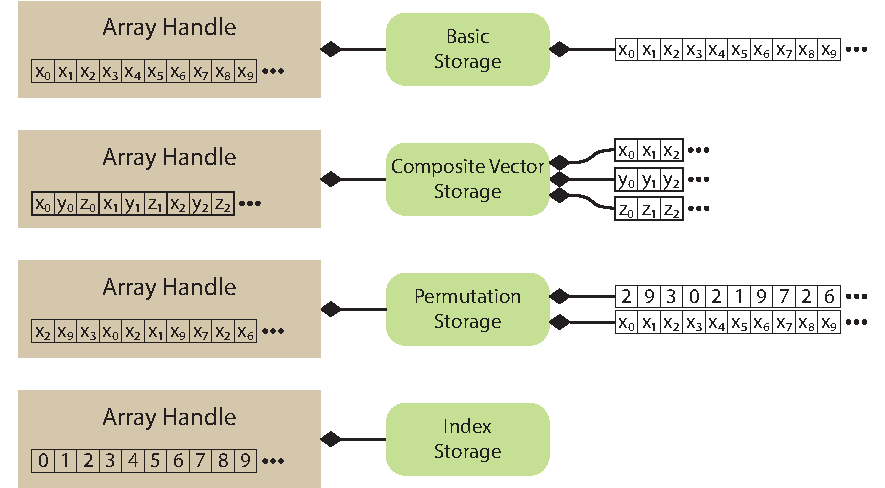
\includegraphics{images/ArrayHandleStorage}
  \caption{Array handles, storage objects, and the underlying data source.}
  \label{fig:ArrayHandleStorage}
\end{figure}

One interesting consequence of using a generic storage object to manage
data within an array handle is that the storage can be defined
functionally rather than point to data stored in physical memory. Thus,
implicit array handles are easily created by adapting to functional
``storage.'' For example, the point coordinates of a uniform rectilinear
grid are implicit based on the topological position of the point. Thus, the
point coordinates for uniform rectilinear grids can be implemented as an
implicit array with the same interface as explicit arrays (where
unstructured grid points would be stored). In this chapter we explore the
many ways you can manipulate the \textidentifier{ArrayHandle} storage.

\begin{didyouknow}
  VTK-m comes with many ``fancy'' array handles that can change the data in
  other arrays without modifying the memory or can generate data on the fly
  to behave like an array without actually using any memory. These fancy
  array handles are documented later in this chapter, and they can be very
  handy when developing with VTK-m.
\end{didyouknow}


\section{Basic Storage}

\index{array handle!storage!default}
\index{storage!default}

As previously discussed in Chapter~\ref{chap:ArrayHandle},
\vtkmcont{ArrayHandle} takes two template arguments.
\begin{vtkmexample}{Declaration of the \protect\vtkmcont{ArrayHandle} templated class (again).}
template<
    typename T,
    typename StorageTag = VTKM_DEFAULT_STORAGE_TAG>
class ArrayHandle;
\end{vtkmexample}
The first argument is the only one required and has been demonstrated
multiple times before. The second (optional) argument specifies something
called a storage, which provides the interface between the generic
\vtkmcont{ArrayHandle} class and a specific storage mechanism in the
control environment.

In this and the following sections we describe this storage mechanism. A
default storage is specified in much the same way as a default device
adapter is defined (as described in Section~\ref{sec:DefaultDeviceAdapter}.
It is done by setting the \vtkmmacro{VTKM\_STORAGE} macro. This macro must
be set before including any VTK-m header files. Currently the only
practical storage provided by VTK-m is the basic storage, which simply
allocates a continuous section of memory of the given base type. This
storage can be explicitly specified by setting \vtkmmacro{VTKM\_STORAGE} to
\vtkmmacro{VTKM\_STORAGE\_BASIC} although the basic storage will also be
used as the default if no other storage is specified (which is typical).

The default storage can always be overridden by specifying an array
storage tag. The tag for the basic storage is located in the
\vtkmheader{vtkm/cont}{StorageBasic.h} header file and is named
\vtkmcont{StorageTagBasic}. Here is an example of specifying
the storage type when declaring an array handle.

\vtkmlisting{Specifying the storage type for an \textidentifier{ArrayHandle.}}{ArrayHandleStorageParameter.cxx}

VTK-m also defines a macro named \vtkmmacro{VTKM\_DEFAULT\_STORAGE\_TAG}
that can be used in place of an explicit storage tag to use the
default tag. This macro is used to create new templates that have template
parameters for storage that can use the default.


\index{array handle!fancy|(}
\index{fancy array handle|(}

\section{Provided Fancy Arrays}
\label{sec:ProvidedFancyArrays}

The generic array handle and storage templating in VTK-m allows for
any type of operations to retrieve a particular value. Typically this is
used to convert an index to some location or locations in memory. However,
it is also possible to do many other operations. Arrays can be augmented on
the fly by mutating their indices or values. Or values could be computed
directly from the index so that no storage is required for the array at
all. This modified behavior for arrays is called ``fancy'' arrays.

VTK-m provides many of the fancy arrays, which we explore in this section.
Later Section~\ref{sec:ImplementingFancyArrays} describes many different
ways in which new fancy arrays can be implemented.

\subsection{Constant Arrays}
\label{sec:ConstantArrays}

\index{array handle!constant|(}
\index{constant array handle|(}

A constant array is a fancy array handle that has the same value in all of
its entries. The constant array provides this array without actually using
any memory.

Specifying a constant array in VTK-m is straightforward. VTK-m has a class
named \vtkmcont{ArrayHandleConstant}. \textidentifier{ArrayHandleConstant}
is a templated class with a single template argument that is the type of
value for each element in the array. The constructor for
\textidentifier{ArrayHandleConstant} takes the value to provide by the
array and the number of values the array should present. The following
example is a simple demonstration of the constant array handle.

\vtkmlisting{Using \textidentifier{ArrayHandleConstant}.}{ArrayHandleConstant.cxx}

The \vtkmheader{vtkm/cont}{ArrayHandleConstant.h} header also contains the
templated convenience function \vtkmcont{make\_ArrayHandleConstant} that
takes a value and a size for the array. This function can sometimes be used
to avoid having to declare the full array type.

\vtkmlisting{Using \textidentifier{make\_ArrayHandleConstant}.}{MakeArrayHandleConstant.cxx}

\index{constant array handle|)}
\index{array handle!constant|)}

\subsection{Counting Arrays}
\label{sec:CountingArrays}

\index{array handle!counting|(}
\index{counting array handle|(}

A counting array is a fancy array handle that provides a sequence of
numbers. These fancy arrays can represent the data without actually using
any memory.

\index{array handle!index|(}
\index{index array handle|(}

VTK-m provides two versions of a counting array. The first version is an
index array that provides a specialized but common form of a counting array
called an index array. An index array has values of type \vtkm{Id} that
start at 0 and count up by 1 (i.e. $0, 1, 2, 3,\ldots$). The index array
mirrors the array's index.

Specifying an index array in VTK-m is done with a class named
\vtkmcont{ArrayHandleIndex}. The constructor for
\textidentifier{ArrayHandleIndex} takes the size of the array to create.
The following example is a simple demonstration of the index array handle.

\vtkmlisting{Using \textidentifier{ArrayHandleIndex}.}{ArrayHandleIndex.cxx}

\index{index array handle|)}
\index{array handle!index|)}

The \vtkmcont{ArrayHandleCounting} class provides a more general form of
counting. \textidentifier{ArrayHandleCounting} is a templated class with a
single template argument that is the type of value for each element in the
array. The constructor for \textidentifier{ArrayHandleCounting} takes three
arguments: the start value (used at index 0), the step from one value to
the next, and the length of the array. The following example is a simple
demonstration of the counting array handle.

\vtkmlisting{Using \textidentifier{ArrayHandleCounting}.}{ArrayHandleCountingBasic.cxx}

\begin{didyouknow}
  In addition to being simpler to declare,
  \textidentifier{ArrayHandleIndex} is slightly faster than
  \textidentifier{ArrayHandleCounting}. Thus, when applicable, you should
  prefer using \textidentifier{ArrayHandleIndex}.
\end{didyouknow}

The \vtkmheader{vtkm/cont}{ArrayHandleCounting.h} header also contains the
templated convenience function \vtkmcont{make\_ArrayHandleCounting} that
also takes the start value, step, and length as arguments. This function
can sometimes be used to avoid having to declare the full array type.

\vtkmlisting{Using \textidentifier{make\_ArrayHandleCounting}.}{MakeArrayHandleCountingBasic.cxx}

There are no fundamental limits on how \textidentifier{ArrayHandleCounting}
counts. For example, it is possible to count backwards.

\vtkmlisting{Counting backwards with \textidentifier{ArrayHandleCounting}.}{ArrayHandleCountingBackward.cxx}

It is also possible to use \textidentifier{ArrayHandleCounting} to make
sequences of \vtkm{Vec} values with piece-wise counting in each of the
components.

\vtkmlisting{Using \textidentifier{ArrayHandleCounting} with \protect\vtkm{Vec} objects.}{ArrayHandleCountingVec.cxx}

\index{counting array handle|)}
\index{array handle!counting|)}

\subsection{Cast Arrays}
\label{sec:CastArrays}

\index{array handle!cast|(}
\index{cast array handle|(}

A cast array is a fancy array that changes the type of the elements in an
array. The cast array provides this re-typed array without actually copying
or generating any data. Instead, casts are performed as the array is
accessed.

VTK-m has a class named \vtkmcont{ArrayHandleCast} to perform this implicit
casting. \textidentifier{ArrayHandleCast} is a templated class with two
template arguments. The first argument is the type to cast values to. The
second argument is the type of the original \textidentifier{ArrayHandle}.
The constructor to \textidentifier{ArrayHandleCast} takes the
\textidentifier{ArrayHandle} to modify by casting.

\vtkmlisting{Using \textidentifier{ArrayHandleCast}.}{ArrayHandleCast.cxx}

The \vtkmheader{vtkm/cont}{ArrayHandleCast.h} header also contains the
templated convenience function \vtkmcont{make\_ArrayHandleCast} that
constructs the cast array. The first argument is the original
\textidentifier{ArrayHandle} original array to cast. The optional second
argument is of the type to cast to (or you can optionally specify the
cast-to type as a template argument.

\vtkmlisting{Using \textidentifier{make\_ArrayHandleCast}.}{MakeArrayHandleCast.cxx}

\index{cast array handle|)}
\index{array handle!cast|)}

\subsection{Discard Arrays}
\label{sec:DiscardArrays}

\index{discard array handle|(}
\index{array handle!discard|(}

It is sometimes the case where you will want to run an operation in \VTKm that fills values in two (or more) arrays, but you only want the values that are stored in one of the arrays.
It is possible to allocate space for both arrays and then throw away the values that you do not want, but that is a waste of memory.
It is also possible to rewrite the functionality to output only what you want, but that is a poor use of developer time.

To solve this problem easily, \VTKm provides \vtkmcont{ArrayHandleDiscard}.
This array behaves similar to a regular \textidentifier{ArrayHandle} in that it can be ``allocated'' and has size, but any values that are written to it are immediately discarded.
\textidentifier{ArrayHandleDiscard} takes up no memory.

\vtkmlisting{Using \textidentifier{ArrayHandleDiscard}.}{ArrayHandleDiscard.cxx}

\index{array handle!discard|)}
\index{discard array handle|)}


\subsection{Permuted Arrays}
\label{sec:PermutedArrays}

\index{array handle!permutation|(}
\index{permuted array handle|(}

A permutation array is a fancy array handle that reorders the elements in
an array. Elements in the array can be skipped over or replicated. The
permutation array provides this reordered array without actually coping any
data. Instead, indices are adjusted as the array is accessed.

Specifying a permutation array in VTK-m is straightforward. VTK-m has a
class named \vtkmcont{ArrayHandlePermutation} that takes two arrays: an
array of values and an array of indices that maps an index in the
permutation to an index of the original values. The index array is
specified first. The following example is a simple demonstration of the
permutation array handle.

\vtkmlisting{Using \textidentifier{ArrayHandlePermutation}.}{ArrayHandlePermutation.cxx}

The \vtkmheader{vtkm/cont}{ArrayHandlePermutation.h} header also contains the
templated convenience function \vtkmcont{make\_ArrayHandlePermutation} that
takes instances of the index and value array handles and returns a
permutation array. This function can sometimes be used to avoid having to
declare the full array type.

\vtkmlisting{Using \textidentifier{make\_ArrayHandlePermutation}.}{MakeArrayHandlePermutation.cxx}

\begin{commonerrors}
  When using an \textidentifier{ArrayHandlePermutation}, take care that all
  the provided indices in the index array point to valid locations in the
  values array. Bad indices can cause reading from or writing to invalid
  memory locations, which can be difficult to debug.
\end{commonerrors}

\begin{didyouknow}
  You can write to a \textidentifier{ArrayHandlePermutation} by, for
  example, using it as an output array. Writes to the
  \textidentifier{ArrayHandlePermutation} will go to the respective
  location in the source array. However,
  \textidentifier{ArrayHandlePermutation} cannot be resized.
\end{didyouknow}

\index{permuted array handle|)}
\index{array handle!permutation|)}

\subsection{Zipped Arrays}
\label{sec:ZippedArrays}

\index{array handle!zip|(}
\index{zipped array handles|(}

A zip array is a fancy array handle that combines two arrays of the same
size to pair up the corresponding values. Each element in the zipped array
is a \vtkm{Pair} containing the values of the two respective arrays. These
pairs are not stored in their own memory space. Rather, the pairs are
generated as the array is used. Writing a pair to the zipped array writes
the values in the two source arrays.

Specifying a zipped array in VTK-m is straightforward. VTK-m has a class
named \vtkmcont{ArrayHandleZip} that takes the two arrays providing values
for the first and second entries in the pairs. The following example is a
simple demonstration of creating a zip array handle.

\vtkmlisting{Using \textidentifier{ArrayHandleZip}.}{ArrayHandleZip.cxx}

The \vtkmheader{vtkm/cont}{ArrayHandleZip.h} header also contains the
templated convenience function \vtkmcont{make\_ArrayHandleZip} that takes
instances of the two array handles and returns a zip array. This function
can sometimes be used to avoid having to declare the full array type.

\vtkmlisting{Using \textidentifier{make\_ArrayHandleZip}.}{MakeArrayHandleZip.cxx}

\index{zipped array handles|)}
\index{array handle!zip|)}

\subsection{Coordinate System Arrays}
\label{sec:CoordinateSystemArrays}

Many of the data structures we use in VTK-m are described in a 3D
coordinate system. Although, as we will see in Chapter~\ref{chap:DataSets},
we can use any \textidentifier{ArrayHandle} to store point coordinates,
including a raw array of 3D vectors, there are some common patterns for
point coordinates that we can use specialized arrays to better represent
the data.

\index{array handle!uniform point coordinates|(}
\index{uniform point coordinates array handle|(}

There are two fancy array handles that each handle a special form of
coordinate system. The first such array handle is
\vtkmcont{ArrayHandleUniformPointCoordinates}, which represents a uniform
sampling of space. The constructor for
\textidentifier{ArrayHandleUniformPointCoordinates} takes three arguments.
The first argument is a \vtkm{Id3} that specifies the number of samples in
the $x$, $y$, and $z$ directions. The second argument, which is optional,
specifies the origin (the location of the first point at the lower left
corner). If not specified, the origin is set to $[0,0,0]$. The third
argument, which is also optional, specifies the distance between samples in
the $x$, $y$, and $z$ directions. If not specified, the spacing is set to
$1$ in each direction.

\vtkmlisting{Using \textidentifier{ArrayHandleUniformPointCoordinates}.}{ArrayHandleUniformPointCoordinates.cxx}

\index{uniform point coordinates array handle|)}
\index{array handle!uniform point coordinates|)}

\index{array handle!Cartesian product|(}
\index{array handle!rectilinear point coordinates|(}
\index{Cartesian product array handle|(}
\index{rectilinear point coordinates array handle|(}

The second fancy array handle for special coordinate systems is
\vtkmcont{ArrayHandleCartesianProduct}, which represents a rectilinear
sampling of space where the samples are axis aligned but have variable
spacing. Sets of coordinates of this type are most efficiently represented
by having a separate array for each component of the axis, and then for
each $[i,j,k]$ index of the array take the value for each component from
each array using the respective index. This is equivalent to performing a
Cartesian product on the arrays.

\textidentifier{ArrayHandleCartesianProduct} is a templated class. It has
three template parameters, which are the types of the arrays used for the
$x$, $y$, and $z$ axes. The constructor for
\textidentifier{ArrayHandleCartesianProduct} takes the three arrays.

\vtkmlisting{Using a \textidentifier{ArrayHandleCartesianProduct}.}{ArrayHandleCartesianProduct.cxx}

The \vtkmheader{vtkm/cont/ArrayHandleCartesianProduct.h} header also
contains the templated convenience function
\vtkmcont{make\_ArrayHandleCartesianProduct} that takes the three axis
arrays and returns an array of the Cartesian product. This function can
sometimes be used to avoid having to declare the full array type.

\vtkmlisting{Using \textidentifier{make\_ArrayHandleCartesianProduct}.}{MakeArrayHandleCartesianProduct.cxx}

\index{rectilinear point coordinates array handle|)}
\index{Cartesian product array handle|)}
\index{array handle!rectilinear point coordinates|)}
\index{array handle!Cartesian product|)}

\begin{didyouknow}
  These specialized arrays for coordinate systems greatly reduce the code
  duplication in VTK-m. Most scientific visualization systems need separate
  implementations of algorithms for uniform, rectilinear, and unstructured
  grids. But in VTK-m an algorithm can be written once and then applied to
  all these different grid structures by using these specialized array
  handles and letting the compiler's templates optimize the code.
\end{didyouknow}

\subsection{Composite Vector Arrays}
\label{sec:CompositeVectorArrays}

\index{array handle!composite vector arrays|(}
\index{composite vector arrays array handle|(}

A composite vector array is a fancy array handle that combines two to four
arrays of the same size and value type and combines their corresponding
values to form a \vtkm{Vec}. A composite vector array is similar in nature
to a zipped array (described in Section~\ref{sec:ZippedArrays}) except that
values are combined into \vtkm{Vec}s instead of \vtkm{Pair}s. The created
\vtkm{Vec}s are not stored in their own memory space. Rather, the
\textidentifier{Vec}s are generated as the array is used. Writing
\textidentifier{Vec}s to the composite vector array writes values into the
components of the source arrays.

A composite vector array can be created using the
\vtkmcont{ArrayHandleCompositeVector} class. This class has a single
template argument that is a ``signature'' for the arrays to be combined.
These signatures can be tricky to prototype, so
\vtkmheader{vtkm/cont/ArrayHandleCompositeVector.h} header also contains a
helper struct named \vtkmcont{ArrayHandleCompositeVectorType} to define the
type. \textidentifier{ArrayHandleCompositeVectorType} takes a variable
number of \textidentifier{ArrayHandle} types that compose the vector.
\textidentifier{ArrayHandleCompositeVectorType} has an internal type named
\textcode{type} that is the appropriately defined
\textidentifier{ArrayHandleCompositeVector}.

The constructor for \textidentifier{ArrayHandleCompositeVector} takes
instances of the array handles to combine along with the component from
each array to use. If the array handles being combined contain scalar data,
then the appropriate component to use is 0.

\vtkmlisting{Using \textidentifier{ArrayHandleCompositeVector}.}{ArrayHandleCompositeVectorBasic.cxx}

The \vtkmheader{vtkm/cont}{ArrayHandleCompositeVector.h} header also
contains the templated convenience function
\vtkmcont{make\_ArrayHandleCompositeVector} which takes two to four array
handles and returns an \textidentifier{ArrayHandleCompositeVector}. This
function can sometimes be used to avoid having to declare the full array
type.

\vtkmlisting{Using \textidentifier{make\_ArrayHandleCompositeVector}.}{MakeArrayHandleCompositeVector.cxx}

\textidentifier{ArrayHandleCompositeVector} is often used to combine scalar
arrays into vector arrays, but it can also be used to pull components out
of other vector arrays. The following example uses this feature to convert
an array of 2D $x,y$ coordinates and an array of elevations to 3D $x,y,z$
coordinates.

\vtkmlisting{Combining vector components with \textidentifier{ArrayHandleCompositeVector}.}{ArrayHandleCompositeVectorComponents.cxx}

\index{composite vector arrays array handle|)}
\index{array handle!composite vector arrays|)}

\subsection{Grouped Vector Arrays}
\label{sec:GroupedVectorArrays}

\index{array handle!group vector|(}
\index{group vector array handle|(}

A grouped vector array is a fancy array handle that groups consecutive
values of an array together to form a \vtkm{Vec}. The source array must be
of a length that is divisible by the requested \textidentifier{Vec} size.
The created \vtkm{Vec}s are not stored in their own memory space. Rather,
the \textidentifier{Vec}s are generated as the array is used. Writing
\textidentifier{Vec}s to the grouped vector array writes values into the
the source array.

A grouped vector array is created using the \vtkmcont{ArrayHandleGroupVec}
class. This templated class has two template arguments. The first argument
is the type of array being grouped and the second argument is an integer
specifying the size of the \textidentifier{Vec}s to create (the number of
values to group together).

\vtkmlisting{Using \textidentifier{ArrayHandleGroupVec}.}{ArrayHandleGroupVecBasic.cxx}

The \vtkmheader{vtkm/cont}{ArrayHandleGroupVec.h} header also contains the
templated convenience function \vtkmcont{make\_ArrayHandleGroupVec} that
takes an instance of the array to group into \textidentifier{Vec}s. You
must specify the size of the \textidentifier{Vec}s as a template parameter
when using \vtkmcont{make\_ArrayHandleGroupVec}.

\vtkmlisting{Using \textidentifier{make\_ArrayHandleGroupVec}.}{MakeArrayHandleGroupVec.cxx}

\textidentifier{ArrayHandleGroupVec} is handy when you need to build an array of vectors that are all of the same length, but what about when you need an array of vectors of different lengths?
One common use case for this is if you are defining a collection of polygons of different sizes (triangles, quadrilaterals, pentagons, and so on).
We would like to define an array such that the data for each polygon were stored in its own \textidentifier{Vec} (or, rather, \Veclike) object.
\vtkmcont{ArrayHandleGroupVecVariable} does just that.

\textidentifier{ArrayHandleGroupVecVariable} takes two arrays. The first array, identified as the ``source'' array, is a flat representation of the values (much like the array used with \textidentifier{ArrayHandleGroupVec}).
The second array, identified as the ``offsets'' array, provides for each vector the index into the source array where the start of the vector is.
The offsets array must be monotonically increasing.
The first and second template parameters to \textidentifier{ArrayHandleGroupVecVariable} are the types for the source and offset arrays, respectively.

It is often the case that you will start with a group of vector lengths rather than offsets into the source array.
If this is the case, then the \vtkmcont{ConvertNumComponentsToOffsets} helper function can convert an array of vector lengths to an array of offsets.
The first argument to this function is always the array of vector lengths.
The second argument, which is optional, is a reference to a \textidentifier{ArrayHandle} into which the offsets should be stored.
If this offset array is not specified, an \textidentifier{ArrayHandle} will be returned from the function instead.
The third argument, which is also optional, is a reference to a \vtkm{Id} into which the expected size of the source array is put.
Having the size of the source array is often helpful, as it can be used to allocate data for the source array or check the source array's size.
It is also OK to give the expected size reference but not the offset array reference.

\vtkmlisting{Using \textidentifier{ArrayHandleGroupVecVariable}.}{ArrayHandleGroupVecVariable.cxx}

The \vtkmheader{vtkm/cont}{ArrayHandleGroupVecVariable.h} header also contains the templated convenience function \vtkmcont{make\_ArrayHandleGroupVecVariable} that takes an instance of the source array to group into \Veclike objects and the offset array.

\vtkmlisting{Using \textidentifier{MakeArrayHandleGroupVecVariable}.}{MakeArrayHandleGroupVecVariable.cxx}

\begin{didyouknow}
  You can write to \textidentifier{ArrayHandleGroupVec} and \textidentifier{ArrayHandleGroupVecVariable} by, for example, using it as an output array.
  Writes to these arrays will go to the respective location in the source array.
  \textidentifier{ArrayHandleGroupVec} can also be allocated and resized (which in turn causes the source array to be allocated).
  However, \textidentifier{ArrayHandleGroupVecVariable} cannot be resized and the source array must be pre-allocated.
  You can use the source array size value returned from \textidentifier{ConvertNumComponentsToOffsets} to allocate source arrays.
\end{didyouknow}

\begin{commonerrors}
  Keep in mind that the values stored in a \textidentifier{ArrayHandleGroupVecVariable} are not actually \vtkm{Vec} objects.
  Rather, they are ``\Veclike'' objects, which has some subtle but important ramifications.
  First, the type will not match the \vtkm{Vec} template, and there is no automatic conversion to \vtkm{Vec} objects.
  Thus, many functions that accept \vtkm{Vec} objects as parameters will not accept the \Veclike object.
  Second, the size of \Veclike objects are not known until runtime.
  See Sections \ref{sec:VectorTypes} and \ref{sec:VectorTraits} for more information on the difference between \vtkm{Vec} and \Veclike objects.
\end{commonerrors}

\index{group vector array handle|)}
\index{array handle!group vector|)}


\section{Implementing Fancy Arrays}
\label{sec:ImplementingFancyArrays}

Although the behavior of fancy arrays might seem complicated, they are
actually straightforward to implement. VTK-m provides several mechanisms to
implement fancy arrays.

\subsection{Implicit Array Handles}

\index{array handle!implicit|(}
\index{storage!implicit|(}
\index{implicit storage|(}
\index{implicit array handle|(}
\index{functional array|(}

The generic array handle and storage templating in VTK-m allows for
any type of operations to retrieve a particular value. Typically this is
used to convert an index to some location or locations in memory. However,
it is also possible to compute a value directly from an index rather than
look up some value in memory. Such an array is completely functional and
requires no storage in memory at all. Such a functional array is called an
\keyterm{implicit array handle}. Implicit arrays are an example of
\keyterm{fancy array handles}, which are array handles that behave like
regular arrays but do special processing under the covers to provide
values.

Specifying a functional or implicit array in VTK-m is straightforward.
VTK-m has a special class named \vtkmcont{ArrayHandleImplicit} that makes
an implicit array containing values generated by a user-specified
\keyterm{functor}. \index{functor} A functor is simply a C++ class or
struct that contains an overloaded parenthesis operator so that it can be
used syntactically like a function.

To demonstrate the use of \textidentifier{ArrayHandleImplicit}, let us say
we want an array of even numbers. The array has the values
$[0,2,4,6,\ldots]$ (double the index) up to some given size. Although we
could easily create this array in memory, we can save space and possibly
time by computing these values on demand.

\begin{didyouknow}
  VTK-m already comes with an implicit array handle named
  \vtkmcont{ArrayHandleCounting} that can make implicit even numbers as
  well as other more general counts. So in practice you would not have to
  create a special implicit array, but we are doing so here for
  demonstrative purposes.
\end{didyouknow}

The first step to using \textidentifier{ArrayHandleImplicit} is to declare
a functor. The functor's parenthesis operator should accept a single
argument of type \vtkm{Id} and return a value appropriate for that index.
The parenthesis operator should also be declared \textcode{const} because
it is not allowed to change the class' state.

\vtkmlisting{Functor that doubles an index.}{ImplicitArrayFunctor.cxx}

Once the functor is defined, an implicit array can be declared using the templated \vtkmcont{ArrayHandleImplicit} class.
The single template argument is the functor's type.

\vtkmlisting{Declaring a \textidentifier{ArrayHandleImplicit}.}{DeclareImplicitArray.cxx}

For convenience, \vtkmheader{vtkm/cont}{ArrayHandleImplicit.h} also
declares the \vtkmcont{make\_ArrayHandleImplicit} function. This function
takes a functor and the size of the array and returns the implicit array.

\vtkmlisting{Using \textidentifier{make\_ArrayHandleImplicit}.}{MakeArrayHandleImplicit.cxx}

\index{array handle!subclassing}

If the implicit array you are creating tends to be generally useful and is
something you use multiple times, it might be worthwhile to make a
convenience subclass of \vtkmcont{ArrayHandleImplicit} for your array.

\vtkmlisting[ex:ImplicitArrayHandleSubclass]{Custom implicit array handle for even numbers.}{ImplicitArrayHandle2.cxx}

Subclasses of \textidentifier{ArrayHandle} provide constructors that
establish the state of the array handle. All array handle subclasses must
also use either the \vtkmmacro{VTKM\_ARRAY\_HANDLE\_SUBCLASS} macro or the
\vtkmmacro{VTKM\_ARRAY\_HANDLE\_SUBCLASS\_NT} macro. Both of these macros
define the typedefs \textcode{Superclass}, \textcode{ValueType}, and
\textcode{StorageTag} as well as a set of constructors and operators
expected of all \textidentifier{ArrayHandle} classes. The difference
between these two macros is that \vtkmmacro{VTKM\_ARRAY\_HANDLE\_SUBCLASS}
is used in templated classes whereas
\vtkmmacro{VTKM\_ARRAY\_HANDLE\_SUBCLASS\_NT} is used in non-templated
classes.

The \textidentifier{ArrayHandle} subclass in
Example~\ref{ex:ImplicitArrayHandleSubclass} is not templated, so it uses
the \vtkmmacro{VTKM\_ARRAY\_HANDLE\_SUBCLASS\_NT} macro. (The other macro
is described in Section~\ref{sec:VTKM_ARRAY_HANDLE_SUBCLASS} on
page~\pageref{sec:VTKM_ARRAY_HANDLE_SUBCLASS}). This macro takes two
parameters. The first parameter is the name of the subclass where the macro
is defined and the second parameter is the immediate superclass including
the full template specification. The second parameter of the macro must be
enclosed in parentheses so that the C pre-processor correctly handles
commas in the template specification.

\index{functional array|)}
\index{implicit array handle|)}
\index{implicit storage|)}
\index{storage!implicit|)}
\index{array handle!implicit|)}

\subsection{Transformed Arrays}
\label{sec:TransformedArrays}

\index{array handle!transform|(}
\index{transformed array|(}

Another type of fancy array handle is the transformed array. A transformed
array takes another array and applies a function to all of the elements to
produce a new array. A transformed array behaves much like a map operation
except that a map operation writes its values to a new memory location
whereas the transformed array handle produces its values on demand so that
no additional storage is required.

Specifying a transformed array in VTK-m is straightforward. VTK-m has a
special class named \vtkmcont{ArrayHandleTransform} that takes an array
handle and a functor and provides an interface to a new array comprising
values of the first array applied to the functor.

To demonstrate the use of \textidentifier{ArrayHandleTransform}, let us say
that we want to scale and bias all of the values in a target array. That
is, each value in the target array is going to be multiplied by a given
scale and then offset by adding a bias value. (The scale and bias are
uniform across all entries.) We could, of course, easily create a worklet
to apply this scale and bias to each entry in the target array and save the
result in a new array, but we can save space and possibly time by computing
these values on demand.

The first step to using \textidentifier{ArrayHandleTransform} is to declare
a functor. The functor's parenthesis operator should accept a single
argument of the type of the target array and return the transformed value.
For more generally applicable transform functors, it is often useful to
make the parenthesis operator a template. The parenthesis operator should
also be declared \textcode{const} because it is not allowed to change the
class' state.

\vtkmlisting{Functor to scale and bias a value.}{TransformArrayFunctor.cxx}

Once the functor is defined, a transformed array can be declared using the templated \vtkmcont{ArrayHandleTransform} class.
The first template argument is the type of array being transformed.
The second template argument is the type of functor used for the transformation.
The third template argument, which is optional, is the type for an inverse functor that provides the inverse operation of the functor in the second argument.
This inverse functor is used for writing values into the array.
For arrays that will only be read from, there is no need to supply this inverse functor.

That said, it is generally easier to use the \vtkmcont{make\_ArrayHandleTransform} convenience function.
This function takes an array and a functor (and optionally an inverse functor) and returns a transformed array.

\vtkmlisting{Using \textidentifier{make\_ArrayHandleTransform}.}{MakeArrayHandleTransform.cxx}

If the transformed array you are creating tends to be generally useful and
is something you use multiple times, it might be worthwhile to make a
convenience subclass of \vtkmcont{ArrayHandleTransform} or convenience
\textcode{make\_ArrayHandle*} function for your array.

\vtkmlisting[ex:TransformArrayHandleSubclass]{Custom transform array handle for scale and bias.}{TransformArrayHandle.cxx}

\label{sec:VTKM_ARRAY_HANDLE_SUBCLASS}

Subclasses of \textidentifier{ArrayHandle} provide constructors that
establish the state of the array handle. All array handle subclasses must
also use either the \vtkmmacro{VTKM\_ARRAY\_HANDLE\_SUBCLASS} macro or the
\vtkmmacro{VTKM\_ARRAY\_HANDLE\_SUBCLASS\_NT} macro. Both of these macros
define the typedefs \textcode{Superclass}, \textcode{ValueType}, and
\textcode{StorageTag} as well as a set of constructors and operators
expected of all \textidentifier{ArrayHandle} classes. The difference
between these two macros is that \vtkmmacro{VTKM\_ARRAY\_HANDLE\_SUBCLASS}
is used in templated classes whereas
\vtkmmacro{VTKM\_ARRAY\_HANDLE\_SUBCLASS\_NT} is used in non-templated
classes.

The \textidentifier{ArrayHandle} subclass in
Example~\ref{ex:TransformArrayHandleSubclass} is templated, so it uses the
\vtkmmacro{VTKM\_ARRAY\_HANDLE\_SUBCLASS} macro. (The other macro is
described in Section~\ref{sec:VTKM_ARRAY_HANDLE_SUBCLASS_NT} on
page~\pageref{sec:VTKM_ARRAY_HANDLE_SUBCLASS_NT}). This macro takes three
parameters. The first parameter is the name of the subclass where the macro
is defined, the second parameter is the type of the subclass including the
full template specification, and the third parameter is the immediate
superclass including the full template specification. The second and third
parameters of the macro must be enclosed in parentheses so that the C
pre-processor correctly handles commas in the template specification.

\index{transformed array|)}
\index{array handle!transform|)}


\subsection{Derived Storage}
\label{sec:DerivedStorage}

\index{array handle!derived|(}
\index{storage!derived|(}
\index{derived storage|(}

A \keyterm{derived storage} is a type of fancy array that takes one or more
other arrays and changes their behavior in some way. A transformed array
(Section~\ref{sec:TransformedArrays}) is a specific type of derived array
with a simple mapping. In this section we will demonstrate the steps
required to create a more general derived storage. When applicable, it is
much easier to create a derived array as a transformed array or using the
other fancy arrays than to create your own derived storage. However, if
these pre-existing fancy arrays do not work work, for example if your
derivation uses multiple arrays or requires general lookups, you can do so
by creating your own derived storage. For the purposes of the example in
this section, let us say we want 2 array handles to behave as one array
with the contents concatenated together. We could of course actually copy
the data, but we can also do it in place.

The first step to creating a derived storage is to build an array portal
that will take portals from arrays being derived. The portal must work in
both the control and execution environment (or have a separate version for
control and execution).

\vtkmlisting[ex:DerivedArrayPortal]{Derived array portal for concatenated arrays.}{DerivedArrayPortal.cxx}

Like in an adapter storage, the next step in creating a derived storage
is to define a tag for the adapter. We shall call ours
\textcode{StorageTagConcatenate} and it will be templated on
the two array handle types that we are deriving. Then, we need to create a
specialization of the templated \vtkmcontinternal{Storage}
class. The implementation for a \textidentifier{Storage} for
a derived storage is usually trivial compared to an adapter storage
because the majority of the work is deferred to the derived arrays.

\vtkmlisting[ex:DerivedArrayStorage]{\textidentifier{Storage} for derived container of concatenated arrays.}{DerivedArrayStorage.cxx}

One of the responsibilities of an array handle is to copy data between the
control and execution environments. The default behavior is to request the
device adapter to copy data items from one environment to another. This
might involve transferring data between a host and device. For an array of
data resting in memory, this is necessary. However, implicit storage
(described in the previous section) overrides this behavior to pass nothing
but the functional array portal. Likewise, it is undesirable to do a raw
transfer of data with derived storage. The underlying arrays being
derived may be used in other contexts, and it would be good to share the
data wherever possible. It is also sometimes more efficient to copy data
independently from the arrays being derived than from the derived storage
itself.

\index{array transfer|(}

The mechanism that controls how a particular storage gets
transferred to and from the execution environment is encapsulated in the
templated \vtkmcontinternal{ArrayTransfer} class. By creating a
specialization of \vtkmcontinternal{ArrayTransfer}, we can modify the
transfer behavior to instead transfer the arrays being derived and use the
respective copies in the control and execution environments.

\vtkmcontinternal{ArrayTransfer} has three template arguments: the base type
of the array, the storage tag, and the device adapter tag.

\vtkmlisting[ex:ArrayTransferPrototype]{Prototype for \protect\vtkmcontinternal{ArrayTransfer}.}{ArrayTransferPrototype.cxx}

All \vtkmcontinternal{ArrayTransfer} implementations must have a
constructor method that accepts a pointer to a \vtkmcontinternal{Storage}
object templated to the same base type and storage tag as the
\textidentifier{ArrayTransfer} object. Assuming that an
\textidentifier{ArrayHandle} is templated using the parameters in
Example~\ref{ex:ArrayTransferPrototype}, the prototype for the constructor
must be equivalent to the following.
\begin{vtkmexample}{Prototype for \textidentifier{ArrayTransfer} constructor.}
ArrayTransfer(vtkm::cont::internal::Storage<T, StorageTag> *storage);
\end{vtkmexample}
Typically the constructor either saves the \textidentifier{Storage} pointer
or other relevant objects from the \textidentifier{Storage} for later use in
the methods.

In addition to this non-default constructor, the
\vtkmcontinternal{ArrayTransfer} specialization must define the following
items.
\begin{description}
\item[\textcode{ValueType}] A \textcode{typedef} of the type for each item
  in the array. This is the same type as the first template argument.
\item[\textcode{PortalControl}] The type of an array portal that is used to
  access the underlying data in the control environment.
\item[\textcode{PortalConstControl}] A read-only (const) version of
  \textcode{PortalControl}.
\item[\textcode{PortalExecution}] The type of an array portal that is used
  to access the underlying data in the execution environment.
\item[\textcode{PortalConstExecution}] A read-only (const) version of
  \textcode{PortalExecution}.
\item[\textcode{GetNumberOfValues}] A method that returns the number of
  values currently allocated in the execution environment. The results may
  be undefined if none of the load or allocate methods have yet been
  called.
\item[\textcode{PrepareForInput}] A method responsible for transferring
  data from the control to the execution for input.
  \textcode{PrepareForInput} has one Boolean argument that controls whether
  this transfer should actually take place. When true, data from the
  \textidentifier{Storage} object given in the constructor should be
  transferred to the execution environment; otherwise the data should not
  be copied. An \textidentifier{ArrayTransfer} for a derived array
  typically ignores this parameter since the arrays being derived manages
  this transfer already. Regardless of the Boolean flag, a
  \textcode{PortalConstExecution} is returned.
\item[\textcode{PrepareForInPlace}] A method that behaves just like
  \textcode{PrepareForInput} except that the data in the execution
  environment is used for both reading and writing so the method returns a
  \textidentifier{PortalExecution}. If the array is considered read-only,
  which is common for derived arrays, then this method should throw a
  \vtkmcont{ErrorControlBadValue}.
\item[\textcode{PrepareForOutput}] A method that takes a size (in a
  \vtkm{Id}) and allocates an array in the execution environment of the
  specified size. The initial memory can be uninitialized. The method
  returns a \textcode{PortalExecution} for the allocated data. If the array
  is considered read-only, which is common for derived arrays, then this
  method should throw a \vtkmcont{ErrorControlBadValue}.
\item[\textcode{RetrieveOutputData}] This method takes an array storage
  pointer (which is the same as that passed to the constructor, but
  provided for convenience), allocates memory in the control environment,
  and copies data from the execution environment into it. If the derived
  array is considered read-only and both \textcode{PrepareForInPlace} and
  \textcode{PrepareForOutput} throw exceptions, then this method should
  never be called. If it is, then that is probably a bug in
  \textidentifier{ArrayHandle}, and it is OK to throw
  \vtkmcont{ErrorControlInternal}.
\item[\textcode{Shrink}] A method that adjusts the size of the array in the
  execution environment to something that is a smaller size. All the data
  up to the new length must remain valid. Typically, no memory is actually
  reallocated. Instead, a different end is marked. If the derived array is
  considered read-only, then this method should throw a
  \vtkmcont{ErrorControlBadValue}.
\item[\textcode{ReleaseResources}] A method that frees any resources
  (typically memory) in the execution environment.
\end{description}

Continuing our example derived storage that concatenates two arrays
started in Examples \ref{ex:DerivedArrayPortal} and
\ref{ex:DerivedArrayStorage}, the following provides an
\textidentifier{ArrayTransfer} appropriate for the derived storage.

\vtkmlisting[ex:DerivedArrayTransfer]{\textidentifier{ArrayTransfer} for derived storage of concatenated arrays.}{DerivedArrayTransfer.cxx}

\index{array transfer|)}

\index{array handle!subclassing}

The final step to make a derived storage is to create a mechanism to
construct an \textidentifier{ArrayHandle} with a storage derived from the
desired arrays. This can be done by creating a trivial subclass of
\vtkmcont{ArrayHandle} that simply constructs the array handle to the state
of an existing storage. It uses a protected constructor of
\vtkmcont{ArrayHandle} that accepts a constructed storage.

\vtkmlisting[ex:DerivedArrayHandle]{\textidentifier{ArrayHandle} for derived storage of concatenated arrays.}{DerivedArrayHandle.cxx}

Subclasses of \textidentifier{ArrayHandle} provide constructors that
establish the state of the array handle. All array handle subclasses must
also use either the \vtkmmacro{VTKM\_ARRAY\_HANDLE\_SUBCLASS} macro or the
\vtkmmacro{VTKM\_ARRAY\_HANDLE\_SUBCLASS\_NT} macro. Both of these macros
define the typedefs \textcode{Superclass}, \textcode{ValueType}, and
\textcode{StorageTag} as well as a set of constructors and operators
expected of all \textidentifier{ArrayHandle} classes. The difference
between these two macros is that \vtkmmacro{VTKM\_ARRAY\_HANDLE\_SUBCLASS}
is used in templated classes whereas
\vtkmmacro{VTKM\_ARRAY\_HANDLE\_SUBCLASS\_NT} is used in non-templated
classes.

The \textidentifier{ArrayHandle} subclass in
Example~\ref{ex:DerivedArrayHandle} is templated, so it uses the
\vtkmmacro{VTKM\_ARRAY\_HANDLE\_SUBCLASS} macro. (The other macro is
described in Section~\ref{sec:VTKM_ARRAY_HANDLE_SUBCLASS_NT} on
page~\pageref{sec:VTKM_ARRAY_HANDLE_SUBCLASS_NT}). This macro takes three
parameters. The first parameter is the name of the subclass where the macro
is defined, the second parameter is the type of the subclass including the
full template specification, and the third parameter is the immediate
superclass including the full template specification. The second and third
parameters of the macro must be enclosed in parentheses so that the C
pre-processor correctly handles commas in the template specification.

\vtkmcont{ArrayHandleCompositeVector} is an example of a derived array
handle provided by VTK-m. It references some fixed number of other arrays,
pulls a specified component out of each, and produces a new component that
is a tuple of these retrieved components.

\index{derived storage|)}
\index{storage!derived|)}
\index{array handle!derived|)}

\index{array handle!fancy|)}
\index{fancy array handle|)}



\section{Adapting Data Structures}
\label{sec:ArrayHandle:Adapting}

\index{array handle!adapting|(}
\index{storage!adapting|(}

The intention of the storage parameter for \vtkmcont{ArrayHandle} is to
implement the strategy design pattern to enable VTK-m to interface directly
with the data of any third party code source. VTK-m is designed to work
with data originating in other libraries or applications. By creating a new
type of storage, VTK-m can be entirely adapted to new kinds of data
structures.

\begin{commonerrors}
  Keep in mind that memory layout used can have an effect on the running
  time of algorithms in VTK-m. Different data layouts and memory access can
  change cache performance and introduce memory affinity problems. The
  example code given in this section will likely have poorer cache
  performance than the basic storage provided by VTK-m. However, that might
  be an acceptable penalty to avoid data copies.
\end{commonerrors}

In this section we demonstrate the steps required to adapt the array handle
to a data structure provided by a third party. For the purposes of the
example, let us say that some fictitious library named ``foo'' has a simple
structure named \textcode{FooFields} that holds the field values for a
particular part of a mesh, and then maintain the field values for all
locations in a mesh in a \textcode{std::deque} object.

\vtkmlisting{Fictitious field storage used in custom array storage examples.}{FictitiousFieldStorage.cxx}

VTK-m expects separate arrays for each of the fields rather than a single
array containing a structure holding all of the fields. However, rather
than copy each field to its own array, we can create a storage for each
field that points directly to the data in a \textcode{FooFieldsDeque}
object.

The first step in creating an adapter storage is to create a control
environment array portal to the data. This is described in more detail in
Section~\ref{sec:ArrayPortals} and is generally straightforward for simple
containers like this. Here is an example implementation for our
\textcode{FooFieldsDeque} container.

\vtkmlisting[ex:ArrayPortalAdapter]{Array portal to adapt a third-party container to VTK-m.}{ArrayPortalAdapter.cxx}

The next step in creating an adapter storage is to define a tag for the
adapter. We shall call ours
\textcode{StorageTagFooPressure}. Then, we need to create a
specialization of the templated \vtkmcontinternal{Storage}
class. The \textidentifier{ArrayHandle} will instantiate an object using
the array container tag we give it, and we define our own specialization so
that it runs our interface into the code.

\vtkmcontinternal{Storage} has two template arguments: the
base type of the array and the storage tag.

\vtkmlisting{Prototype for \protect\vtkmcontinternal{Storage}.}{StoragePrototype.cxx}

The \vtkmcontinternal{Storage} must define the following items.
\begin{description}
\item[\textcode{ValueType}] A \textcode{typedef} of the type for each item
  in the array. This is the same type as the first template argument.
\item[\textcode{PortalType}] The type of an array portal that can be used
  to access the underlying data. This array portal needs to work only in
  the control environment.
\item[\textcode{PortalConstType}] A read-only (const) version of
  \textcode{PortalType}.
\item[\textcode{GetPortal}] A method that returns an array portal of type
  \textcode{PortalType} that can be used to access the data manged in this
  storage.
\item[\textcode{GetPortalConst}] Same as \textcode{GetPortal} except it
  returns a read-only (const) array portal.
\item[\textcode{GetNumberOfValues}] A method that returns the number of
  values the storage is currently allocated for.
\item[\textcode{Allocate}] A method that allocates the array to a given
  size. An values stored in the previous allocation may be destroyed.
\item[\textcode{Shrink}] A method like \textcode{Allocate} with two
  differences. First, the size of the allocation must be smaller than the
  existing allocation when the method is called. Second, any values
  currently stored in the array will be valid after the array is
  resized. This constrained form of allocation allows the array to be
  resized and values valid without ever having to copy data.
\item[\textcode{ReleaseResources}] A method that instructs the storage to
  free all of its memory.
\end{description}

The following provides an example implementation of our adapter to a
\textcode{FooFieldsDeque}. It relies on the
\textcode{ArrayPortalFooPressure} provided in
Example~\ref{ex:ArrayPortalAdapter}.

\vtkmlisting{Storage to adapt a third-party container to VTK-m.}{StorageAdapter.cxx}

\index{array handle!subclassing}

The final step to make a storage adapter is to make a mechanism to
construct an \textidentifier{ArrayHandle} that points to a particular
storage. This can be done by creating a trivial subclass of
\vtkmcont{ArrayHandle} that simply constructs the array handle to the state
of an existing container.

\vtkmlisting[ex:ArrayHandleAdapter]{Array handle to adapt a third-party container to VTK-m.}{ArrayHandleAdapter.cxx}

\label{sec:VTKM_ARRAY_HANDLE_SUBCLASS_NT}

Subclasses of \textidentifier{ArrayHandle} provide constructors that
establish the state of the array handle. All array handle subclasses must
also use either the \vtkmmacro{VTKM\_ARRAY\_HANDLE\_SUBCLASS} macro or the
\vtkmmacro{VTKM\_ARRAY\_HANDLE\_SUBCLASS\_NT} macro. Both of these macros
define the typedefs \textcode{Superclass}, \textcode{ValueType}, and
\textcode{StorageTag} as well as a set of constructors and operators
expected of all \textidentifier{ArrayHandle} classes. The difference
between these two macros is that \vtkmmacro{VTKM\_ARRAY\_HANDLE\_SUBCLASS}
is used in templated classes whereas
\vtkmmacro{VTKM\_ARRAY\_HANDLE\_SUBCLASS\_NT} is used in non-templated
classes.

The \textidentifier{ArrayHandle} subclass in
Example~\ref{ex:ArrayHandleAdapter} is not templated, so it uses
the \vtkmmacro{VTKM\_ARRAY\_HANDLE\_SUBCLASS\_NT} macro. (The other macro
is described in Section~\ref{sec:VTKM_ARRAY_HANDLE_SUBCLASS} on
page~\pageref{sec:VTKM_ARRAY_HANDLE_SUBCLASS}). This macro takes two
parameters. The first parameter is the name of the subclass where the macro
is defined and the second parameter is the immediate superclass including
the full template specification. The second parameter of the macro must be
enclosed in parentheses so that the C pre-processor correctly handles
commas in the template specification.

With this new version of \textidentifier{ArrayHandle}, VTK-m can now read
to and write from the \textcode{FooFieldsDeque} structure directly. Note,
however, that when writing to an array handle, it is necessary to call
\textcode{GetPortalControl} or \textcode{GetPortalConstControl} to flush
data from the execution environment to the control environment. \fix{Should
  probably make this easier.}

\vtkmlisting{Using an \textidentifier{ArrayHandle} with custom container.}{UsingArrayHandleAdapter.cxx}

\index{array handle!storage!default}
\index{storage!default}

Most of the code in VTK-m will create \textidentifier{ArrayHandle}s using
the default storage, which is set to the basic storage if not otherwise
specified. If you wish to replace the default storage used, then set the
\vtkmmacro{VTKM\_STORAGE} macro to \vtkmmacro{VTKM\_STORAGE\_UNDEFINED} and
set the \vtkmmacro{VTKM\_DEFAULT\_STORAGE\_TAG} to your tag class. These
definitions have to happen \emph{before} including any VTK-m header files.
You will also have to declare the tag class (or at least a prototype of it)
before including VTK-m header files.

\begin{vtkmexample}{Redefining the default array handle storage.}
#define VTKM_STORAGE VTKM_STORAGE_UNDEFINED
#define VTKM_DEFAULT_STORAGE_TAG StorageTagFooPressure

struct StorageTagFooPressure;
\end{vtkmexample}

\begin{commonerrors}
  \textidentifier{ArrayHandle}s are often stored in dynamic objects like
  dynamic arrays (Chapter~\ref{chap:DynamicArrayHandle}) or data sets
  (Chapter~\ref{chap:DataSets}). When this happens, the array's type
  information, including the storage used, is lost. VTK-m will have to
  guess the storage, and if you do not tell VTK-m to try your custom
  storage, you will get a runtime error when the array is used. The most
  common ways of doing this are to change the default storage tag
  (described here), adding the storage tag to the default storage list
  (Section~\ref{sec:DynamicArrayHandleSpecifyingCastLists}) or specifying
  the storage tag in the policy when executing filters (\fix{Add reference
    when documented.}).
\end{commonerrors}

\index{storage!adapting|)}
\index{array handle!adapting|)}



\index{storage|)}
\index{array handle!storage|)}

\index{array handle|)}


  % -*- latex -*-

\chapter{Dynamic Array Handles}
\label{chap:DynamicArrayHandle}

\index{dynamic array handle|(}
\index{array handle!dynamic|(}

The \textidentifier{ArrayHandle} class uses templating to make very
efficient and type-safe access to data. However, it is sometimes
inconvenient or impossible to specify the element type and storage at
run-time. The \textidentifier{DynamicArrayHandle} class provides a mechanism
to manage arrays of data with unspecified types.

\vtkmcont{DynamicArrayHandle} holds a reference to an array. Unlike
\textidentifier{ArrayHandle}, \textidentifier{DynamicArrayHandle} is
\emph{not} templated. Instead, it uses C++ run-type type information to
store the array without type and cast it when appropriate.

\index{dynamic array handle!construct}
A \textidentifier{DynamicArrayHandle} can be established by constructing it
with or assigning it to an \textidentifier{ArrayHandle}. The following
example demonstrates how a \textidentifier{DynamicArrayHandle} might be
used to load an array whose type is not known until run-time.

\vtkmlisting{Creating a \textidentifier{DynamicArrayHandle}.}{CreateDynamicArrayHandle.cxx}

\section{Querying and Casting}
\label{sec:DynamicArrayHandleQueryingAndCasting}

\index{dynamic array handle!query}
Data pointed to by a \textidentifier{DynamicArrayHandle} is not directly
accessible. However, there are a few generic queries you can make without
directly knowing the data type. The \textcode{GetNumberOfValues} method
returns the length of the array with respect to its base data type. It is
also common in VTK-m to use data types, such as \vtkm{Vec}, with multiple
components per value. The \textcode{GetNumberOfComponents} method returns
the number of components in a vector-like type (or 1 for scalars).

\vtkmlisting{Non type-specific queries on \textidentifier{DynamicArrayHandle}.}{NonTypeQueriesDynamicArrayHandle.cxx}

\index{dynamic array handle!new instance}
It is also often desirable to create a new array based on the underlying
type of a \textidentifier{DynamicArrayHandle}. For example, when a filter
creates a field, it is common to make this output field the same type as
the input. To satisfy this use case, \textidentifier{DynamicArrayHandle}
has a method named \textcode{NewInstance} that creates a new empty array
with the same underlying type as the original array.

\vtkmlisting{Using \textidentifier{DynamicArrayHandle}\textcode{::NewInstance()}.}{DynamicArrayHandleNewInstance.cxx}

Before the data with a \textidentifier{DynamicArrayHandle} can be accessed,
the type and storage of the array must be established. This is usually done
internally within VTK-m when a worklet \fix{or filter?} is invoked.
However, it is also possible to query the types and cast to a concrete
\textidentifier{ArrayHandle}.

\index{dynamic array handle!query}
You can query the component type and storage type using the
\textcode{IsType}, \textcode{IsSameType}, and
\textcode{IsTypeAndStorage} methods. \textcode{IsType} takes an
example array handle type and returns whether the underlying array matches
the given static array type. \textcode{IsSameType} behaves the same as
\textcode{IsType} but accepts an instance of an
\textidentifier{ArrayHandle} object to automatically resolve the template
parameters. \textcode{IsTypeAndStorage} takes an example
component type and an example storage type as arguments and returns whether
the underlying array matches both types.

\vtkmlisting{Querying the component and storage types of a \textidentifier{DynamicArrayHandle}.}{QueryDynamicArrayHandle.cxx}

\index{dynamic array handle!cast}
Once the type of the \textidentifier{DynamicArrayHandle} is known, it can
be cast to a concrete \textidentifier{ArrayHandle}, which has access to the
data as described in Chapter~\ref{chap:ArrayHandle}. The easiest way to do
this is to use the \textcode{CopyTo} method. This templated method takes a
reference to an \textidentifier{ArrayHandle} as an argument and sets that
array handle to point to the array in \textidentifier{DynamicArrayHandle}.
If the given types are incorrect, then \textcode{CopyTo} throws
a \vtkmcont{ErrorControlBadValue} exception.

\vtkmlisting{Casting a \textidentifier{DynamicArrayHandle} to a concrete
  \textidentifier{ArrayHandle}.}{CastDynamicArrayHandle.cxx}

\begin{commonerrors}
  Remember that \textidentifier{ArrayHandle} and
  \textidentifier{DynamicArrayHandle} represent pointers to the data, so
  this ``copy'' is a shallow copy. There is still only one copy of the
  data, and if you change the data in one array handle that change is
  reflected in the other. 
\end{commonerrors}

\section{Casting to Unknown Types}

\index{dynamic array handle!cast|(}

Using \textcode{CopyTo} is fine as long as the correct types are
known, but often times they are not. For this use case
\textidentifier{DynamicArrayHandle} has a method named
\textcode{CastAndCall} that attempts to cast the array to some set of
types.

The \textcode{CastAndCall} method accepts a functor to run on the
appropriately cast array. The functor must have an overloaded const
parentheses operator that accepts an \textidentifier{ArrayHandle} of the
appropriate type.

\vtkmlisting[ex:UsingCastAndCall]{Operating on \textidentifier{DynamicArrayHandle} with \textcode{CastAndCall}.}{UsingCastAndCall.cxx}

\begin{commonerrors}
  It is possible to store any form of \textidentifier{ArrayHandle} in a
  \textidentifier{DynamicArrayHandle}, but it is not possible for
  \textcode{CastAndCall} to check every possible form of
  \textidentifier{ArrayHandle}. If \textcode{CastAndCall} cannot determine
  the \textidentifier{ArrayHandle} type, then an
  \textidentifier{ErrorControlBadValue} is thrown. The following section
  describes how to specify the forms of \textidentifier{ArrayHandle} to try.
\end{commonerrors}

\section{Specifying Cast Lists}
\label{sec:DynamicArrayHandleSpecifyingCastLists}

The \textcode{CastAndCall} method can only check a finite number of types.
The default form of \textcode{CastAndCall} uses a default set of common
types. These default lists can be overridden using the VTK-m list tags
facility, which is discussed at length in Section~\ref{sec:ListTags}. There
are separate lists for value types and for storage types.

Common type lists for value are defined in
\vtkmheader{vtkm}{TypeListTag.h} and are documented in
Section~\ref{sec:TypeLists}. This header also defines
\vtkmmacro{VTKM\_DEFAULT\_TYPE\_LIST\_TAG}, which defines the default list
of value types tried in \textcode{CastAndCall}.

\index{tag!storage lists|(}
\index{lists!storage|(}
\index{storage lists|(}

Common storage lists are defined in
\vtkmheader{vtkm/cont}{StorageListTag.h}. There is only one common storage
distributed with VTK-m: \textidentifier{StorageBasic}. A list tag
containing this type is defined as \vtkmcont{StorageListTagBasic}.

As with other lists, it is possible to create new storage type lists
using the existing type lists and the list bases from
Section~\ref{sec:BuildingListTags}.

The \vtkmheader{vtkm/cont}{StorageListTag.h} header also defines a macro
named \vtkmmacro{VTKM\_DEFAULT\_STORAGE\_LIST\_TAG} that defines a
default list of types to use in classes like
\textidentifier{DynamicArrayHandle}. This list can be overridden by
defining the \vtkmmacro{VTKM\_DEFAULT\_STORAGE\_LIST\_TAG} macro
\emph{before} any VTK-m headers are included. If included after a VTK-m
header, the list is not likely to take effect. Do not ignore compiler
warnings about the macro being redefined, which you will not get if defined
correctly.

\index{storage lists|)}
\index{lists!storage|)}
\index{tag!storage lists|)}

There is a form of \textcode{CastAndCall} that accepts tags for the list of
component types and storage types. This can be used when the specific
lists are known at the time of the call. However, when creating generic
operations like the \textcode{PrintArrayContents} function in
Example~\ref{ex:UsingCastAndCall}, passing these tags is inconvenient at
best.

To address this use case, \textidentifier{DynamicArrayHandle} has a pair of
methods named \textcode{ResetTypeList} and
\textcode{ResetStorageList}. These methods return a new object with that
behaves just like a \textidentifier{DynamicArrayHandle} with identical
state except that the cast and call functionality uses the specified
component type or storage type instead of the default. (Note that
\textcode{PrintArrayContents} in Example~\ref{ex:UsingCastAndCall} is
templated on the type of \textidentifier{DynamicArrayHandle}. This is to
accommodate using the objects from the \textcode{Reset*List} methods, which
have the same behavior but different type names.)

So the default component type list contains a subset of the basic VTK-m
types. If you wanted to accommodate more types, you could use
\textcode{ResetTypeList}.

\vtkmlisting{Trying all component types in a \textidentifier{DynamicArrayHandle}.}{CastAndCallAllTypes.cxx}

Likewise, if you happen to know a particular type of the dynamic array,
that can be specified to reduce the amount of object code created by
templates in the compiler.

\vtkmlisting{Specifying a single component type in a \textidentifier{DynamicArrayHandle}.}{CastAndCallSingleType.cxx}

Storage type lists can be changed similarly.

\vtkmlisting{Specifying different storage types in a \textidentifier{DynamicArrayHandle}.}{CastAndCallStorage.cxx}

\begin{commonerrors}
  The \textcode{ResetTypeList} and \textcode{ResetStorageList} do not
  change the object they are called on. Rather, they return a new object
  with different type information. Calling these methods has no effect
  unless you do something with the returned value.
\end{commonerrors}

Both the component type list and the storage type list can be modified by
chaining these reset calls.

\vtkmlisting{Specifying both component and storage types in a \textidentifier{DynamicArrayHandle}.}{CastAndCallTypeAndStorage.cxx}

The \textcode{ResetTypeList} and \textcode{ResetStorageList} work by
returning a \vtkmcont{DynamicArrayHandleBase} object.
\textidentifier{DynamicArrayHandleBase} specifies the value and storage tag
lists as template arguments and otherwise behaves just like
\textidentifier{DynamicArrayHandle}.

\begin{didyouknow}
  I lied earlier when I said at the beginning of this chapter that
  \textidentifier{DynamicArrayHandle} is a class that is not templated.
  This symbol is really just a \textcode{typedef} of
  \textidentifier{DynamicArrayHandleBase}. Because the
  \textidentifier{DynamicArrayHandle} fully specifies the template
  arguments, it behaves like a class, but if you get a compiler error it
  will show up as \textidentifier{DynamicArrayHandleBase}.
\end{didyouknow}

Most code does not need to worry about working directly with
\textidentifier{DynamicArrayHandleBase}. However, it is sometimes useful to
declare it in templated functions that accept dynamic array handles so that
works with every type list. The function in
Example~\ref{ex:UsingCastAndCall} did this by making the dynamic array
handle class itself the template argument. This will work, but it is prone
to error because the template will resolve to any type of argument. When
passing objects that are not dynamic array handles will result in strange
and hard to diagnose errors. Instead, we can define the same function using
\textidentifier{DyamicArrayHandleBase} so that the template will only match
dynamic array handle types.

\vtkmlisting{Using \textidentifier{DynamicArrayHandleBase} to accept generic dynamic array handles.}{DynamicArrayHandleBase.cxx}


\index{dynamic array handle!cast|)}

\index{array handle!dynamic|)}
\index{dynamic array handle|)}


  % -*- latex -*-

\chapter{Data Sets}
\label{chap:DataSets}
\label{chap:DataSet}

\index{data~set|(}

A \keyterm{data set}, implemented with the \vtkmcont{DataSet} class,
contains and manages the geometric data structures that VTK-m operates on.
A data set comprises the following 3 data structures.

\begin{description}
\item[Cell Set] \index{cell~set} A cell set describes topological
  connections. A cell set defines some number of points in space and how
  they connect to form cells, filled regions of space. A data set must have
  at least one cell set, but can have more than one cell set defined. This
  makes it possible to define groups of cells with different properties.
  For example, a simulation might model some subset of elements as boundary
  that contain properties the other elements do not. Another example is the
  representation of a molecule that requires atoms and bonds, each having
  very different properties associated with them.
\item[Field] \index{field} A field describes numerical data associated with
  the topological elements in a cell set. The field is represented as an
  array, and each entry in the field array corresponds to a topological
  element (point, edge, face, or cell). Together the cell set topology and
  discrete data values in the field provide an interpolated function
  throughout the volume of space covered by the data set. A cell set can
  have any number of fields.
\item[Coordinate System] \index{coordinate~system} A coordinate system is a
  special field that describes the physical location of the points in a
  data set. Although it is most common for a data set to contain a single
  coordinate system, VTK-m supports data sets with no coordinate system
  such as abstract data structures like graphs that might not have
  positions in a space. \textidentifier{DataSet} also supports multiple
  coordinate systems for data that have multiple representations for
  position. For example, geospatial data could simultaneously have
  coordinate systems defined by 3D position, latitude-longitude, and any
  number of 2D projections.
\end{description}

\section{Building Data Sets}
\label{sec:DataSets:Building}

\index{data~set!Building|(}

Before we go into detail on the cell sets, fields, and coordinate systems
that make up a data set in VTK-m, let us first discuss how to build a data
set. One simple way to build a data set is to load data from a file using
the \vtkmio{} module. Reading files is discussed in detail in
Chapter~\ref{chap:FileIO}.

This section describes building data sets of different types using a set of
classes named \textcode{DataSetBuilder*}, which provide a convenience layer
on top of \vtkmcont{DataSet} to make it easier to create data sets.

\subsection{Creating Uniform Grids}

\index{uniform~grid}
\index{regular~grid}
\index{image}

Uniform grids are meshes that have a regular array structure with points
uniformly spaced parallel to the axes. Uniform grids are also sometimes
called regular grids or images.

The \vtkmcont{DataSetBuilderUniform} class can be used to easily create 2-
or 3-dimensional uniform grids. \textidentifier{DataSetBuilderUniform} has
several versions of a method named \textcode{Create} that takes the number
of points in each dimension, the origin, and the spacing. The origin is the
location of the first point of the data (in the lower left corner), and the
spacing is the distance between points in the x, y, and z directions. The
\textcode{Create} methods also take an optional name for the coordinate
system and an optional name for the cell set.

The following example creates a \vtkmcont{DataSet} containing a uniform
grid of $101 \times 101 \times 26$ points.

\vtkmlisting{Creating a uniform grid.}{CreateUniformGrid.cxx}

If not specified, the origin will be at the coordinates $(0,0,0)$ and the
spacing will be $1$ in each direction. Thus, in the previous example the
width, height, and depth of the mesh in physical space will be $100$,
$100$, and $25$, respectively, and the mesh will be centered at $(50, 50,
12.5)$. Let us say we actually want a mesh of the same dimensions, but we
want the $z$ direction to be stretched out so that the mesh will be the
same size in each direction, and we want the mesh centered at the origin.

\vtkmlisting{Creating a uniform grid with custom origin and spacing.}{CreateUniformGridCustomOriginSpacing.cxx}

\subsection{Creating Rectilinear Grids}

\index{rectilinear~grid}

A rectilinear grid is similar to a uniform grid except that a rectilinear
grid can adjust the spacing between adjacent grid points. This allows the
rectilinear grid to have tighter sampling in some areas of space, but the
points are still constrained to be aligned with the axes and each other. The
irregular spacing of a rectilinear grid is specified by providing a
separate array each for the x, y, and z coordinates.

The \vtkmcont{DataSetBuilderRectilinear} class can be used to easily create
2- or 3-dimensional rectilinear grids.
\textidentifier{DataSetBuilderRectilinear} has several versions of a method
named \textcode{Create} that takes these coordinate arrays and builds a
\vtkmcont{DataSet} out of them. The arrays can be supplied as either
standard C arrays or as \textcode{std::vector} objects, in which case the
data in the arrays are copied into the \textidentifier{DataSet}. These
arrays can also be passed as \textidentifier{ArrayHandle} objects, in which
case the data are shallow copied.

The following example creates a \vtkmcont{DataSet} containing a rectilinear
grid with $201 \times 201 \times 101$ points with different irregular
spacing along each axis.

\vtkmlisting{Creating a rectilinear grid.}{CreateRectilinearGrid.cxx}

\subsection{Creating Explicit Meshes}

\index{explicit~mesh}
\index{unstructured~grid}

An explicit mesh is an arbitrary collection of cells with arbitrary
connections. It can have multiple different types of cells. Explicit meshes
are also known as unstructured grids.

The cells of an explicit mesh are defined by providing the shape, number of
indices, and the points that comprise it for each cell. These three things
are stored in separate arrays. Figure~\ref{fig:ExplicitMesh} shows an
example of an explicit mesh and the arrays that can be used to define it.

\begin{figure}[htb]
  \centering
  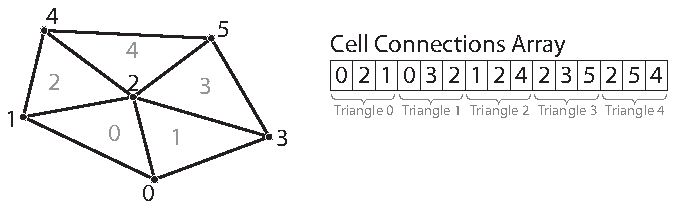
\includegraphics{images/ExplicitCellConnections}
  \caption{An example explicit mesh.}
  \label{fig:ExplicitMesh}
\end{figure}

The \vtkmcont{DataSetBuilderExplicit} class can be used to create data sets
with explicit meshes. \textidentifier{DataSetBuilderExplicit} has several
versions of a method named \textcode{Create}. Generally, these methods take
the shapes, number of indices, and connectivity arrays as well as an array
of point coordinates. These arrays can be given in \textcode{std::vector}
objects, and the data are copied into the \textidentifier{DataSet} created.

The following example creates a mesh like the one shown in
Figure~\ref{fig:ExplicitMesh}.

\vtkmlisting{Creating an explicit mesh with \textidentifier{DataSetBuilderExplicit}.}{CreateExplicitGrid.cxx}

Often it is awkward to build your own arrays and then pass them to
\textidentifier{DataSetBuilderExplicit}. There also exists an alternate
builder class named \vtkmcont{DataSetBuilderExplicitIterative} that allows
you to specify each cell and point one at a time rather than all at once.
This is done by calling one of the versions of \textcode{AddPoint} and one
of the versions of \textcode{AddCell} for each point and cell,
respectively. The next example also builds the mesh shown in
Figure~\ref{fig:ExplicitMesh} except this time using
\textidentifier{DataSetBuilderExplicitIterative}.

\vtkmlisting{Creating an explicit mesh with \textidentifier{DataSetBuilderExplicitIterative}.}{CreateExplicitGridIterative.cxx}

\subsection{Add Fields}

In addition to creating the geometric structure of a data set, it is
usually important to add fields to the data. Fields describe numerical data
associated with the topological elements in a cell. They often represent a
physical quantity (such as temperature, mass, or volume fraction) but can
also represent other information (such as indices or classifications).

The easiest way to define fields in a data set is to use the
\vtkmcont{DataSetFieldAdd} class. This class works on
\textidentifier{DataSet}s of any type. It has methods named
\textcode{AddPointField} and \textcode{AddCellField} that define a field
for either points or cells. Every field must have an associated field name.

Both \textcode{AddPointField} and \textcode{AddCellField} are overloaded to
accept arrays of data in different structures. Field arrays can be passed
as standard C arrays or as \textcode{std::vector}s, in which case the data
are copied. Field arrays can also be passed in a
\textidentifier{ArrayHandle}, in which case the data are not copied.

The following (somewhat contrived) example defines fields for a uniform
grid that identify which points and cells are on the boundary of the mesh.

\vtkmlisting{Adding fields to a \textidentifier{DataSet}.}{AddFieldData.cxx}

\index{data~set!Building|)}

\section{Cell Sets}
\label{sec:DataSets:CellSets}

\index{cell~set|(}
\index{data~set!cell~set|see{cell~set}}

A cell set determines the topological structure of the data in a data set.
Fundamentally, any cell set is a collection of cells, which typically (but
not always) represent some region in space. 3D cells are made up of
\index{point}\index{shape!point}\index{cell!point}points,
\index{edge}\index{shape!edge}\index{cell!edge}edges, and
\index{face}\index{shape!face}\index{cell!face}faces. (2D cells have only points and edges,
and 1D cells have only points.) Figure~\ref{fig:CellTopology} shows the
relationship between a cell's shape and these topological elements. The
arrangement of these points, edges, and faces is defined by the
\index{shape}\index{cell~set!shape}\index{cell~shape}\keyterm{shape} of the
cell, which prescribes a specific ordering of each. The basic cell shapes
provided by VTK-m are discussed in detail in
Section~\ref{sec:CellShapeTagsIds} starting on
page~\pageref{sec:CellShapeTagsIds}.

\begin{figure}[htb]
  \centering
  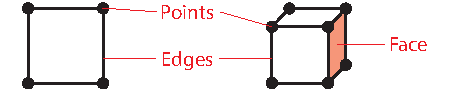
\includegraphics{images/CellConstituents}
  \caption{The relationship between a cell shape and its topological
    elements (points, edges, and faces).}
  \label{fig:CellTopology}
\end{figure}

There are multiple ways to express the connections of a cell set, each with
different benefits and restrictions. These different cell set types are
managed by different cell set classes in VTK-m. All VTK-m cell set classes
inherit from \vtkmcont{CellSet}. The two basic types of cell sets are
structured and explicit, and there are several variations of these types.

\subsection{Structured Cell Sets}

\index{cell~set!structured|(}
\index{structured~cell~set|(}

A \vtkmcont{CellSetStructured} defines a 1-, 2-, or 3-dimensional grid of
points with lines, quadrilaterals, or hexahedra, respectively, connecting
them. The topology of a \textidentifier{CellSetStructured} is specified by
simply providing the dimensions, which is the number of points in the $i$,
$j$, and $k$ directions of the grid of points. The number of points is
implicitly $i \times j \times k$ and the number of cells is implicitly
$(i-1) \times (j-1) \times (k-1)$ (for 3D grids).
Figure~\ref{fig:CellSetStructured} demonstrates this arrangement.

\begin{figure}[htb]
  \centering
  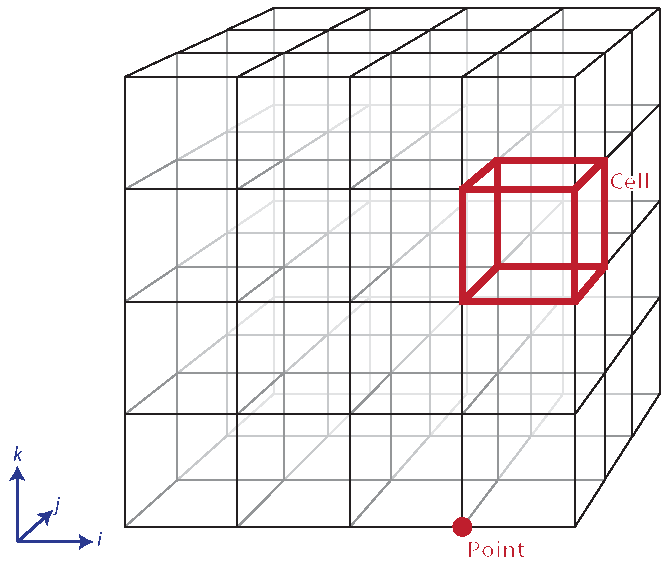
\includegraphics{images/StructuredCellSet}
  \caption{The arrangement of points and cells in a 3D structured grid.}
  \label{fig:CellSetStructured}
\end{figure}

The big advantage of using \vtkmcont{CellSetStructured} to define a cell
set is that it is very space efficient because the entire topology can be
defined by the three integers specifying the dimensions. Also algorithms
can be optimized for \textidentifier{CellSetStructured}'s regular nature.
However, \textidentifier{CellSetStructured}'s strictly regular grid
structure also limits its applicability. A structured cell set can only be
a dense grid of lines, quadrilaterals, or hexahedra. It cannot represent
irregular data well.

Many data models in other software packages, such as the one for VTK, make
a distinction between uniform, rectilinear, and curvilinear grids. VTK-m's
cell sets do not. All three of these grid types are represented by
\textidentifier{CellSetStructured}. This is because in a VTK-m data set the
cell set and the coordinate system are defined independently and used
interchangeably. A structured cell set with uniform point coordinates makes
a uniform grid. A structured cell set with point coordinates defined
irregularly along coordinate axes makes a rectilinear grid. And a
structured cell set with arbitrary point coordinates makes a curvilinear
grid. The point coordinates are defined by the data set's coordinate system,
which is discussed in Section~\ref{sec:DataSets:CoordinateSystems} starting
on page~\pageref{sec:DataSets:CoordinateSystems}.

\index{structured~cell~set|)}
\index{cell~set!structured|)}

\subsection{Explicit Cell Sets}

\index{explicit~cell~set|(}
\index{cell~set!explicit|(}

A \vtkmcont{CellSetExplicit} defines an irregular collection of cells. The
cells can be of different types and connected in arbitrary ways. This is
done by explicitly providing for each cell a sequence of points that
defines the cell.

An explicit cell set is defined with a minimum of three arrays. The first
array identifies the shape of each cell. (Cell shapes are discussed in
detail in Section~\ref{sec:CellShapeTagsIds} starting on
page~\pageref{sec:CellShapeTagsIds}.) The second array identifies how many
points are in each cell. The third array has a sequence of point indices
that make up each cell. Figure~\ref{fig:CellSetExplicit} shows a simple
example of an explicit cell set.

\begin{figure}[htb]
  \centering
  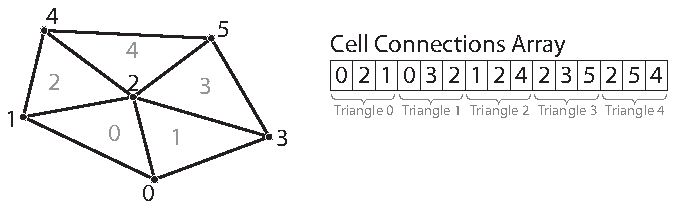
\includegraphics{images/ExplicitCellConnections}
  \caption{Example of cells in a \textidentifier{CellSetExplict} and the
    arrays that define them.}
  \label{fig:CellSetExplicit}
\end{figure}

An explicit cell set may also have other topological arrays such as an
array of offsets of each cell into the connectivity array or an array of
cells incident on each point. Although these arrays can be provided, they
are optional and can be internally derived from the shape, num indices, and
connectivity arrays.

\vtkmcont{ExplicitCellSet} is a powerful representation for a cell set
because it can represent an arbitrary collection of cells. However, because
all connections must be explicitly defined,
\textidentifier{ExplicitCellSet} requires a significant amount of memory to
represent the topology.

\index{cell~set!single~type|(}
\index{explicit~cell~set!single~type|(}
\index{single~type~cell~set|(}

An important specialization of an explicit cell set is
\vtkmcont{CellSetSingleType}. \textidentifier{CellSetSingleType} is an
explicit cell set constrained to contain cells that all have the same shape
and all have the same number of points. So for example if you are creating
a surface that you know will contain only triangles,
\textidentifier{CellSetSingleType} is a good representation for these data.

Using \textidentifier{CellSetSingleType} saves memory because the array of
cell shapes and the array of point counts no longer need to be stored.
\textidentifier{CellSetSingleType} also allows VTK-m to skip some
processing and other storage required for general explicit cell sets.

\index{single~type~cell~set|)}
\index{explicit~cell~set!single~type|)}
\index{cell~set!single~type|)}

\index{cell~set!explicit|)}
\index{explicit~cell~set|)}

\subsection{Cell Set Permutations}

\index{permutation~cell~set|(}
\index{cell~set!permutation|(}

A \vtkmcont{CellSetPermutation} rearranges the cells of one cell set to
create another cell set. This restructuring of cells is not done by copying
data to a new structure. Rather, \textidentifier{CellSetPermutation}
establishes a look-up from one cell structure to another. Cells are permuted
on the fly while algorithms are run.

A \textidentifier{CellSetPermutation} is established by providing a mapping
array that for every cell index provides the equivalent cell index in the
cell set being permuted. \textidentifier{CellSetPermutation} is most often
used to mask out cells in a data set so that algorithms will skip over
those cells when running.

\begin{didyouknow}
  Although \textidentifier{CellSetPermutation} can mask cells, it cannot
  mask points. All points from the original cell set are available in the
  permuted cell set regardless of whether they are used.
\end{didyouknow}

The following example uses \vtkmcont{CellSetPermutation} with a counting
array to expose every tenth cell. This provides a simple way to subsample a
data set.

\vtkmlisting{Subsampling a data set with \textidentifier{CellSetPermutation}.}{CreateCellSetPermutation.cxx}

\index{cell~set!permutation|)}
\index{permutation~cell~set|)}

\subsection{Dynamic Cell Sets}

\index{dynamic~cell~set|(}
\index{cell~set!dynamic|(}

\vtkmcont{DataSet} must hold an arbitrary collection of \vtkmcont{CellSet}
objects, which it cannot do while knowing their types at compile time. To
manage storing \textidentifier{CellSet}s without knowing their types,
\textidentifier{DataSet} actually holds references using
\vtkmcont{DynamicCellSet}.

\textidentifier{DynamicCellSet} is similar in nature to
\textidentifier{DynamicArrayHandle} except that it, of course, holds
\textidentifier{CellSet}s instead of \textidentifier{ArrayHandle}s. The
interface for the two classes is similar, and you should review the
documentation for \textidentifier{DynamicArrayHandle} (in
Chapter~\ref{chap:DynamicArrayHandle} starting on
page~\pageref{chap:DynamicArrayHandle}) to understand
\textidentifier{DynamicCellSet}.

\vtkmcont{DynamicCellSet} has a method named \textcode{GetCellSet} that
returns a const reference to the held cell set as the abstract
\textidentifier{CellSet} class. This can be used to easily access the
virtual methods in the \textidentifier{CellSet} interface. You can also
create a new instance of a cell set with the same type using the
\textcode{NewInstance} method.

The \textidentifier{DynamicCellSet}\textcode{::IsType()} method can be used
to determine whether the cell set held in the dynamic cell set is of a
given type. If the cell set type is known,
\textidentifier{DynamicCellSet}\textcode{::CastTo()} can be used to safely
downcast the cell set object.

When a typed version of the cell set stored in the
\textidentifier{DynamicCellSet} is needed but the type is not known, which
happens regularly in the internal workings of VTK-m, the
\textcode{CastAndCall} method can be used to make this transition.
\textcode{CastAndCall} works by taking a functor and calls it with the
appropriately cast cell set object.

The \textcode{CastAndCall} method works by attempting to cast to a known
set of types. This set of types used is defined by the macro
\vtkmmacro{VTKM\_DEFAULT\_CELL\_SET\_LIST\_TAG}, which is declared in
\vtkmheader{vtkm/cont}{CellSetListTag.h}. This list can be overridden
globally by defining the \vtkmmacro{VTKM\_DEFAULT\_CELL\_SET\_LIST\_TAG}
macro \emph{before} any VTK-m headers are included.

The set of types used in a \textcode{CastAndCall} can also be changed only
for a particular instance of a dynamic cell set by calling its
\textcode{ResetCellSetList}. This method takes a list of cell types and
returns a new dynamic array handle of a slightly different type that will
use this new list of cells for dynamic casting.

\index{cell~set!dynamic|)}
\index{dynamic~cell~set|}

\subsection{Blocks and Assemblies}

Rather than just one cell set, a \vtkmcont{DataSet} can hold multiple cell
sets. This can be used to construct multiblock data structures or
assemblies of parts. Multiple cell sets can also be used to represent
subsets of the data with particular properties such as all cells filled
with a material of a certain type. Or these multiple cells might represent
particular features in the data, such as the set of faces representing a
boundary in the simulation.

\subsection{Zero Cell Sets}

It is also possible to construct a \vtkmcont{DataSet} that contains no cell
set objects whatsoever. This can be used to manage data that does not
contain any topological structure. For example, a collection of series that
come from columns in a table could be stored as multiple fields in a data
set with no cell set.

\index{cell~set|)}

\section{Fields}
\label{sec:DataSets:Fields}

\index{field|(}
\index{data~set!field|see{field}}

A field on a data set provides a value on every point in space on the mesh.
Fields are often used to describe physical properties such as pressure,
temperature, mass, velocity, and much more. Fields are represented in a
VTK-m data set as an array where each value is associated with a particular
element type of a mesh (such as points or cells). This association of field
values to mesh elements and the structure of the cell set determines how
the field is interpolated throughout the space of the mesh.

Fields are manged by the \vtkmcont{Field} class. \textidentifier{Field}
holds its data with a \textidentifier{DynamicArrayHandle}, which itself is
a container for an \textidentifier{ArrayHandle}. \textidentifier{Field}
also maintains the association and, optionally, the name of a cell set for
which the field is valid.

The data array can be retrieved as a \textidentifier{DynamicArrayHandle}
using the \textcode{GetData} method of \textidentifier{Field}.
\textidentifier{Field} also has a convenience method named
\textcode{GetBounds} that finds the range of values stored in the field
array.

\index{field|}

\section{Coordinate Systems}
\label{sec:DataSets:CoordinateSystems}

\index{coordinate~system|(}
\index{data~set!coordinate~system|see{coordinate~system}}

A coordinate system determines the location of a mesh's elements in space.
The spatial location is described by providing a 3D vector at each point
that gives the coordinates there. The point coordinates can then be
interpolated throughout the mesh.

Coordinate systems are managed by the \vtkmcont{CoordinateSystem} class. In
actuality, a coordinate system is just a field with a special meaning, and
so the \textidentifier{CoordinateSystem} class inherits from the
\textidentifier{Field} class. \textidentifier{CoordinateSystem} constrains
the field to be associated with points and typically has 3D floating point
vectors for values.

It is typical for a \textidentifier{DataSet} to have one coordinate system
defined, but it is possible to define multiple coordinate systems. This is
helpful when there are multiple ways to express coordinates. For example,
positions in geographic may be expressed as Cartesian coordinates or as
latitude-longitude coordinates. Both are valid and useful in different
ways.

It is also valid to have a \textidentifier{DataSet} with no coordinate
system. This is useful when the structure is not rooted in physical space.
For example, if the cell set is representing a graph structure, there might
not be any physical space that has meaning for the graph.

\index{coordinate~system|)}

\index{data~set|)}


  % -*- latex -*-

\chapter{Filter Polices}
\label{chap:FilterPolicies}
\label{chap:Policies}

\index{filter!policies|(}
\index{policies|(}

In Chapter~\ref{chap:ProvidedFilters} we explored the set of filter classes in \VTKm, which provide a convenient interface for running the algorithms that come with \VTKm.
That chapter describes methods like \textcode{Execute} and \textcode{MapFieldOntoOutput}, which take data process it in parallel.
What is not described in Chapter~\ref{chap:ProvidedFilters} is how the filter chooses data types and what computing device (e.g. CPU or GPU) to use.

These decisions are determined by \keyterm{policies}.
A policy defines the behavior of how a filter interprets dynamic data and what devices it should use.
The methods previously described in~\ref{chap:ProvidedFilters} implicitly use a default policy that tries the most common types and a group of basic devices.
However, each of these methods have an alternate form that allows you to specify a customized policy.
In this chapter we describe policies and demonstrate how to create and use your own policies.


\section{Default Policy}

\index{filter!policies!default|(}
\index{policies!default|(}

The default policy is specified by the \vtkmfilter{DefaultPolicy} class, which is defined in the \vtkmheader{vtkm/filter}{DefaultPolicy.h} header file.
The default policy can be used any place a standard policy is used, although generally this is unnecessary as the default policy is used automatically if no policy is specified.

\begin{didyouknow}
  The \vtkmfilter{DefaultPolicy} class makes for a good reference on what a policy contains and how to construct a new policy.
  The contents of the default policy can also be used when creating new policies where only some of the properties need be different (as is done in the examples here).
\end{didyouknow}

\fix{It would be nice if you could create a new policy that inherited all of the default policies rather than require you to define every one. If that were implemented, then the description above would change as would pretty much all the examples here.}

\index{policies!default|)}
\index{filter!policies!default|)}


\section{Policy Contents}
\label{sec:PolicyContents}

A policy is a traits-like object that contains the following typedefs.
\fix{Most of?} These typedefs are list tag objects.
List tags are described in Section~\ref{sec:ListTags}.

\begin{description}
\item[\textcode{FieldTypeList}] \index{FieldTypeList}
  A type list tag containing a list of all possible types of values in field arrays used as input to the filter.
  The default policy sets this to \vtkmmacro{VTKM\_DEFAULT\_TYPE\_LIST\_TAG}, which corresponds to \vtkm{Int32}, \vtkm{Int64}, \vtkm{Float32}, \vtkm{Float64}, \vtkm{Vec}\tparams{\vtkm{Float32},3}, and \vtkm{Vec}\tparams{\vtkm{Float64},3}.
\item[\textcode{FieldStorageList}] \index{FieldStorageList}
  A type list tag containing a list of all possible storage types for field arrays used as input to the filter.
  The default policy sets this to \vtkmmacro{VTKM\_DEFAULT\_STORAGE\_LIST\_TAG}, which corresponds to a list containing only \vtkmcont{StorageTagBasic} (the default storage for \vtkmcont{ArrayHandle} objects).
\item[\textcode{CoordinateTypeList}] \index{CoordinateTypeList}
  A type list tag containing a list of all possible types of values in field arrays used as input to the filter when the field array comes from the coordinates of the data set.
  The default policy sets this to \vtkmmacro{VTKM\_DEFAULT\_COORDINATE\_SYSTEM\_TYPE\_LIST\_TAG}, which corresponds to \vtkm{Vec}\tparams{\vtkm{Float32},3} and \vtkm{Vec}\tparams{\vtkm{Float64},3}.
\item[\textcode{CoordinateStorageList}] \index{CoordinateStorageList}
  A type list tag containing a list of all possible storage types for field arrays used as input to the filter when the field array comes from the coordinates of the data set.
  The default policy sets this to \vtkmmacro{VTKM\_DEFAULT\_COORDINATE\_SYSTEM\_STORAGE\_LIST\_TAG}, which corresponds to a list containing the basic \textidentifier{ArrayHandle} storage as well as structures for \vtkmcont{ArrayHandleUniformPointCoordinates}, \vtkmcont{ArrayHandleCompositeVector}, and \vtkmcont{ArrayHandleCartesianProduct}.
\item[\textcode{StructuredCellSetList}] \index{StructuredCellSetList}
  A type list tag containing a list of all possible cell sets classes used when representing structured cell sets.
  The default policy sets this to \vtkmcont{CellSetListTagStructured}, which corresponds to a list containing \vtkmcont{CellSetStructured}\tparams{2} and \vtkmcont{CellSetStructured}\tparams{3}.
\item[\textcode{UnstructuredCellSetList}] \index{UnstructuredCellSetList}
  A type list tag containing a list of all possible cell set classes used when representing unstructured cell sets.
  The default policy sets this to \vtkmcont{CellSetListTagUnstructured}, which corresponds to a list containing \vtkmcont{CellSetExplicit} and \vtkmcont{CellSetSingleType}.
\item[\textcode{AllCellSetList}] \index{AllCellSetList}
  A type list tag containing a list of all possible cell set classes.
  This is usually a union of \textcode{StructuredCellSetList} and \textcode{UnstructuredCellSetList}.
  The default policy sets this to \vtkmmacro{VTKM\_DEFAULT\_CELL\_SET\_LIST\_TAG}, which corresponds to a list containing \vtkmcont{CellSetStructured}\tparams{2}, \vtkmcont{CellSetStructured}\tparams{3}, \vtkmcont{CellSetExplicit}, and \vtkmcont{CellSetSingleType}
\item[\textcode{DeviceAdapterList}] \index{DeviceAdapterList}
  A type list tag containing a list of device adapter tags for the devices to try to run the algorithm on.
  The devices are tried in the order they are listed in \textcode{DeviceAdapterList}, so the ``best'' devices should be listed first.
  The default policy sets this to \vtkmmacro{VTKM\_DEFAULT\_DEVICE\_ADAPTER\_LIST\_TAG}, which corresponds to a list containing \vtkmcont{DeviceAdapterTagCuda}, \vtkmcont{DeviceAdapterTagTBB}, and \vtkmcont{DeviceAdapterTagSerial}.
\end{description}

\begin{commonerrors}
  Just because a device is listed in \textcode{DeviceAdapterList} there is no guarantee that such a device will ever be used.
  For example, if the Cuda device is listed (as in the default) but the filter is not compiled by the Cuda compiler, then that device will always be skipped.
\end{commonerrors}


\section{Creating Policies}

\index{filter!policies!custom|(}
\index{policies!custom|(}

Creating a policy is as simple as creating a subclass of \vtkmfilter{PolicyBase} that provides typedefs for each of the expected policy information types.
\textidentifier{PolicyBase} is a templated class that takes as its single template parameter the type of the subclass.
For example, a policy object named \textcode{PolicyFoo} will subclass \textidentifier{PolicyBase}\tparams{PolicyFoo}.

\begin{didyouknow}
  The convention of having a subclass be templated on the derived class' type is known as the Curiously Recurring Template Pattern (CRTP).
  In the case of policies, \VTKm uses this CRTP behavior to allow methods to have templates that accept any policy type but nothing that is not a policy.
\end{didyouknow}

After inheriting from \textidentifier{PolicyBase}, the custom policy class adds definitions for the type names listed in Section~\ref{sec:PolicyContents}.
The following examples show type typical structure for some common instances of policies.
Although these custom policies are separated by use case, there is no real restriction on combining them.

\fix{The \VTKm source is moving from using \textcode{typedef} to \textcode{using =}. Perhaps we should go through and change all of the examples.}

\fix{Maybe I will hold off on implementing this. If the virtual method branch gets accepted, then the policies will change significantly.}

\index{policies!custom|)}
\index{filter!policies!custom|)}

\index{policies|)}
\index{filter!policies|)}


}{}

\ifthenelse{\equal{\buildtype}{Full} \OR \equal{\buildtype}{Developing}}{

  \part{Developing with VTK-m}
  \label{part:Developing}

  % -*- latex -*-

\chapter{Worklets}
\label{chap:Worklets}

\index{worklet|(}

The simplest way to implement an algorithm in VTK-m is to create a
\keyterm{worklet}. A worklet is fundamentally a functor that operates on an
element of data. Thus, it is a \textcode{class} or \textcode{struct} that
has an overloaded parenthesis operator (which must be declared
\textcode{const} for thread safety). However, worklets are also embedded
with a significant amount of metadata on how the data should be managed and
how the execution should be structured. This chapter explains the basic
mechanics of defining and using worklets.


\section{Worklet Types}
\label{sec:WorkletTypes}

\index{worklet~types|(}

Different operations in visualization can have different data access
patterns, perform different execution flow, and require different
provisions. VTK-m manages these different accesses, execution, and
provisions by grouping visualization algorithms into common classes of
operation and supporting each class with its own worklet type.

Each worklet type has a generic superclass that worklets of that particular
type must inherit. This makes the type of the worklet easy to identify. The
following list describes each worklet type provided by VTK-m and the
superclass that supports it. Details on how to create worklets of each type
are given in Section~\ref{sec:WorkletTypeReference}. It is also possible
to create new worklet types in VTK-m. This is an advanced topic covered in
Chapter~\ref{chap:AdvancedWorklets}.

\begin{description}
\item[Field Map] \index{worklet~types!field~map} \index{field~map~worklet}
  A worklet deriving \vtkmworklet{WorkletMapField} performs a basic mapping
  operation that applies a function (the operator in the worklet) on all
  the field values at a single point or cell and creates a new field value
  at that same location. Although the intention is to operate on some
  variable over a mesh, a \textidentifier{WorkletMapField} may actually be
  applied to any array. Thus, a field map can be used as a basic
  \index{map}map operation.

\item[Topology Map] \index{worklet~types!topology~map}
  \index{topology~map~worklet} A worklet deriving
  \vtkmworklet{WorkletMapTopology} or one of its sibling classes performs a
  mapping operation that applies a function (the operator in the worklet)
  on all elements of a particular type (such as points or cells) and
  creates a new field for those elements. The basic operation is similar to
  a field map except that in addition to access fields being mapped on, the
  worklet operation also has access to incident fields.

  There are multiple convenience classes available for the most common
  types of topology mapping. \index{worklet~types!point~to~cell}
  \index{point~to~cell~worklet} \vtkmworklet{WorkletMapPointToCell} calls
  the worklet operation for each cell and makes every incident point
  available. This type of map also has access to cell structures and can
  interpolate point fields.
  %% \index{worklet~types!cell~to~point}
  %% \index{cell~to~point~worklet} \vtkmworklet{WorkletMapCellToPoint} calls
  %% the worklet operation for each point and makes every incident cell
  %% available.
\end{description}

\index{worklet~types|)}


\section{Dispatchers}
\label{sec:Dispatchers}

\index{dispatcher|(}

Worklets, both those provided by VTK-m as listed in
Section~\ref{sec:ProvidedWorklets} and ones created by a user as described
in Section~\ref{sec:CreatingWorklets}, are instantiated in the control
environment and run in the execution environment. This means that the
control environment must have a means to \index{invoke}\keyterm{invoke}
worklets that start running in the execution environment.

This invocation is done through a set of
\index{dispatcher}\keyterm{dispatcher} objects. A dispatcher object is an
object in the control environment that has an instance of a worklet and can
invoke that worklet with a set of arguments. There are multiple types of
dispatcher objects, each corresponding to a type of worklet object. All
dispatcher objects have at least two template parameters: the worklet class
being invoked, which is always the first argument, and the device adapter
tag, which is always the last argument and will be set to the default
device adapter if not specified.

All dispatcher classes have a method named \textcode{Invoke} that launches
the worklet in the execution environment.  The arguments to
\textcode{Invoke} must match those expected by the worklet, which is
specified by something called a \keyterm{control signature}. The expected
arguments for worklets provided by VTK-m are documented in
Section~\ref{sec:ProvidedWorklets}. Also, for any worklet, the
\textcode{Invoke} arguments can be gleaned from the control signature,
which is described in Section~\ref{sec:ControlSignature}.

The following is a list of the dispatchers defined in VTK-m. The
dispatcher classes correspond to the list of worklet types specified in
Section~\ref{sec:WorkletTypes}. Many examples of using these dispatchers
are provided in Section~\ref{sec:ProvidedWorklets}.

\begin{description}
\item[\vtkmworklet{DispatcherMapField}] The dispatcher used in conjunction
  with a worklet that subclasses \vtkmworklet{WorkletMapField}. The
  dispatcher class has two template arguments: the worklet type and the
  device adapter (optional).
\item[\vtkmworklet{DispatcherMapTopology}] The dispatcher used in
  conjunction with a worklet that subclasses
  \vtkmworklet{WorkletMapTopology} or one of its sibling classes (such as
  \vtkmworklet{WorkletMapPointToCell}). The dispatcher class has two
  template arguments: the worklet type and the device adapter (optional).
%% \item[\daxcont{DispatcherMapCell}] The dispatcher used in conjunction with
%%   a worklet that subclasses \dax{WorkletMapCell}. The class has two
%%   template arguments: the worklet type and the device adapter (optional).
%% \item[\daxcont{DispatcherGenerateTopology}] The dispatcher used in
%%   conjunction with a worklet that subclasses
%%   \dax{WorkletGenerateTopology}. The class has three template arguments: the
%%   worklet type, the type of array handle containing the count of the number
%%   of cells being generated (optional), and the device adapter
%%   (optional). The default type of the count array handle is
%%   \daxcont{ArrayHandle}\textcode{<}\dax{Id}\textcode{>}. An instance of the
%%   count array handle must be provided in the constructor of
%%   \daxcont{DispatcherGenerateTopology}.
%% \item[\daxcont{DispatcherInterpolatedCell}] The dispatcher used in
%%   conjunction with a worklet that subclasses
%%   \dax{WorkletInterpolatedCell}. The class has three template arguments: the
%%   worklet type, the type of array handle containing the count of the number
%%   of cells being generated (optional), and the device adapter
%%   (optional). The default type of the count array handle is
%%   \daxcont{ArrayHandle}\textcode{<}\dax{Id}\textcode{>}. An instance of the
%%   count array handle must be provided in the constructor of
%%   \daxcont{DispatcherInterpolatedCell}.
%% \item[\daxcont{DispatcherGenerateKeysValues}] The dispatcher used in
%%   conjunction with a worklet that subclasses
%%   \dax{WorkletGenerateKeysValues}. The class has three template arguments:
%%   the worklet type, the type of array handle containing the count of the
%%   number of key-values being generated (optional), and the device adapter
%%   (optional). The default type of the count array handle is
%%   \daxcont{ArrayHandle}\textcode{<}\dax{Id}\textcode{>}. An instance of the
%%   count array handle must be provided in the constructor of
%%   \daxcont{DispatcherGenerateKeysValues}.
%% \item[\daxcont{DispatcherReduceKeysValues}] The dispatcher used in
%%   conjunction with a worklet that subclasses
%%   \dax{WorkletReduceKeysValues}. The class has three template arguments:
%%   the worklet type, the type of array handle containing the keys
%%   (optional), and the device adapter (optional). The default type of the
%%   key array handle is
%%   \daxcont{ArrayHandle}\textcode{<}\dax{Id}\textcode{>}. An instance of the
%%   key array handle must be provided in the constructor of
%%   \daxcont{DispatcherReduceKeysValues}.
\end{description}

\index{dispatcher|)}

\section{Provided Worklets}
\label{sec:ProvidedWorklets}

\VTKm comes with several worklet implementations.
These worklet implementations for the most part provide the underlying implementations of the filters described in Chapter~\ref{chap:ProvidedFilters}.
The easiest way to execute a filter is to run it from the associated filter class.
However, if your data is not in a \vtkmcont{DataSet} structure or you have knowledge of the specific data types used in the \textidentifier{DataSet}, it might be more efficient to run the worklet directly.
Note that many of the filters use multiple worklets under the covers to implement the full functionality.

The following example demonstrates using the simple \vtkmworklet{PointElevation} worklet directly.

\vtkmlisting{Using the provided \textidentifier{PointElevation} worklet.}{UsePointElevationWorklet.cxx}


\section{Creating Worklets}
\label{sec:CreatingWorklets}

\index{worklet!creating|(}

A worklet is created by implementing a \textcode{class} or
\textcode{struct} with the following features.

\begin{enumerate}
\item The class must contain a \controlsignature \textcode{typedef}, which
  specifies what arguments are expected when invoking the class with a
  dispatcher in the control environment.
\item The class must contain an \executionsignature \textcode{typedef},
  which specifies how the data gets passed from the arguments in the
  control environment to the worklet running in the execution environment.
\item The class must contain an \inputdomain \textcode{typedef}, which
  identifies which input parameter defines the input domain of the data.
\item The class may define a scatter operation to override a 1:1 mapping
  from input to output.
\item The class must contain an overload of the parenthesis operator, which
  is the method that is executed in the execution environment.
\item The class must publicly inherit from a base worklet class that
  specifies the type of operation being performed.
\end{enumerate}

Figure~\ref{fig:WorkletExampleAnnotated} demonstrates all of the required
components of a worklet.

%% \pagebreak
%% \begin{vtkmexample}{Example Code for Cutting/Pasting.}
%% class TriangulateCell : public vtkm::worklet::WorkletMapPointToCell
%% {
%% public:
%%   typedef void ControlSignature(CellSetIn topology,
%%                                 ExecObject tables,
%%                                 FieldOutCell<> connectivityOut);
%%   typedef void ExecutionSignature(CellShape, PointIndices, _2, _3, VisitIndex);
%%   typedef _1 InputDomain;

%%   typedef vtkm::worklet::ScatterCounting ScatterType;
%%   VTKM_CONT
%%   ScatterType GetScatter() const
%%   {
%%     return this->Scatter;
%%   }

%%   template<typename CellShapeTag,
%%            typename ConnectivityInVec,
%%            typename ConnectivityOutVec>
%%   VTKM_EXEC
%%   void operator()(
%%       CellShapeTag shape,
%%       const ConnectivityInVec &connectivityIn,
%%       const internal::TriangulateTablesExecutionObject<DeviceAdapter> &tables,
%%       ConnectivityOutVec &connectivityOut,
%%       vtkm::IdComponent visitIndex) const
%%   {
%% \end{vtkmexample}
%% \pagebreak

\begin{figure}[htb]
  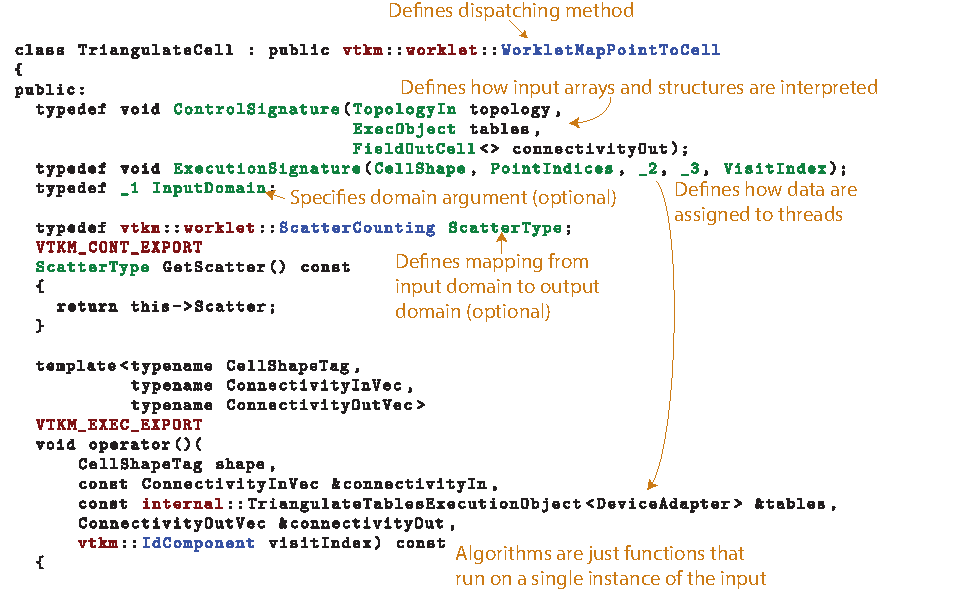
\includegraphics[width=\linewidth]{images/WorkletExampleAnnotated}
  \caption{Annotated example of a worklet declaration.}
  \label{fig:WorkletExampleAnnotated}
\end{figure}

\subsection{Control Signature}
\label{sec:ControlSignature}

\index{control~signature|(}
\index{signature!control|(}
\index{worklet!control~signature|(}

The control signature of a worklet is the \textcode{typedef} of a function
prototype named \controlsignature. The function prototype matches the
calling specification used with the dispatcher \textcode{Invoke} function.

\vtkmlisting{A \protect\controlsignature.}{ControlSignature.cxx}

The return type of the function prototype is always \textcode{void} because
the dispatcher \textcode{Invoke} functions do not return values. The
parameters of the function prototype are \index{signature tags}\keyterm{tags}
that identify the type of data that is expected to be passed to invoke.
\controlsignature tags are defined by the worklet type and the various tags
are documented more fully in Section~\ref{sec:WorkletTypeReference}.

By convention, \controlsignature tag names start with the base concept
(e.g. \textsignature{Field} or \textsignature{Topology}) followed by the
domain (e.g. \textsignature{Point} or \textsignature{Cell}) followed by
\textsignature{In} or \textsignature{Out}. For example,
\sigtag{FieldPointIn} would specify values for a field on the points of a
mesh that are used as input (read only). Although they should be there in
most cases, some tag names might leave out the domain or in/out parts if
they are obvious or ambiguous.

\subsubsection{Type List Tags}
\label{sec:TypeListTags}

\index{type~list~tags|(}
\index{control~signature!type~list~tags|(}

Some tags are templated to have modifiers. For example,
\textsignature{Field} tags have a template argument that is set to a type
list tag defining what types of field data are supported. (See
Section~\ref{sec:TypeLists} for a description of type lists.) In fact, this
type list modifier is so common that the following convenience subtags used
with \textsignature{Field} tags are defined for all worklet types.

\begin{didyouknow}
  Any type list will work as modifiers for \controlsignature tags. However,
  these common type lists are provided for convenience and to make the
  \controlsignature shorter and more readable.
\end{didyouknow}

\begin{description}
  \label{TypeTagList}
\item[\sigtag{AllTypes}] All possible types.
\item[\sigtag{CommonTypes}] The most used types in visualization. This
  includes signed integers and floats that are 32 or 64 bit. It also
  includes 3 dimensional vectors of floats. The same as
  \vtkm{TypeListTagCommon}.
\item[\sigtag{IdType}] Contains the single item \vtkm{Id}. The same as
  \vtkm{TypeListTagId}.
\item[\sigtag{Id2Type}] Contains the single item \vtkm{Id2}. The same as
  \vtkm{TypeListTagId2}.
\item[\sigtag{Id3Type}] Contains the single item \vtkm{Id3}. The same as
  \vtkm{TypeListTagId3}.
\item[\sigtag{Index}] All types used to index arrays. Contains \vtkm{Id},
  \vtkm{Id2}, and \vtkm{Id3}. The same as \vtkm{TypeListTagIndex}.
\item[\sigtag{FieldCommon}] A list containing all the types generally
  used for fields. It is the combination of \sigtag{Scalar}, \sigtag{Vec2},
  \sigtag{Vec3}, and \sigtag{Vec4}. The same as \vtkm{TypeListTagField}.
\item[\sigtag{Scalar}] Types used for scalar fields. Specifically, it
  contains floating point numbers of different widths (i.e. \vtkm{Float32}
  and \vtkm{Float64}). The same as \vtkm{TypeListTagFieldScalar}.
\item[\sigtag{ScalarAll}] All scalar types. It contains signed and unsigned
  integers of widths from 8 to 64 bits. It also contains floats of 32 and
  64 bit widths. The same as \vtkm{TypeListTagScalarAll}.
\item[\sigtag{Vec2}] Types for values of fields with 2 dimensional
  vectors. All these vectors use floating point numbers. The same as
  \vtkm{TypeListTagFieldVec2}.
\item[\sigtag{Vec3}] Types for values of fields with 3 dimensional
  vectors. All these vectors use floating point numbers. The same as
  \vtkm{TypeListTagFieldVec3}.
\item[\sigtag{Vec4}] Types for values of fields with 4 dimensional
  vectors. All these vectors use floating point numbers. The same as
  \vtkm{TypeListTagFieldVec4}.
\item[\sigtag{VecAll}] All \vtkm{Vec} classes with standard integers or
  floating points as components and lengths between 2 and 4. The same as
  \vtkm{TypeListTagVecAll}.
\item[\sigtag{VecCommon}] The most common vector types. It contains all
  \vtkm{Vec} class of size 2 through 4 containing components of unsigned
  bytes, signed 32-bit integers, signed 64-bit integers, 32-bit floats, or
  64-bit floats. The same as \vtkm{TypeListTagVecCommon}.
\end{description}

\index{control~signature!type~list~tags|)}
\index{type~list~tags|)}

\index{worklet!control~signature|)}
\index{signature!control|)}
\index{control~signature|)}

\subsection{Execution Signature}
\label{sec:ExecutionSignature}

\index{execution~signature|(}
\index{signature!execution|(}
\index{worklet!execution~signature|(}

Like the control signature, the execution signature of a worklet is the
\textcode{typedef} of a function prototype named \executionsignature. The
function prototype must match the parenthesis operator (described in
Section~\ref{sec:WorkletOperator}) in terms of arity and argument
semantics.

\vtkmlisting{An \protect\executionsignature.}{ExecutionSignature.cxx}

The arguments of the \executionsignature's function prototype are tags that
define where the data come from. The most common tags are an underscore
followed by a number, such as \sigtagnum{1}, \sigtagnum{2}, etc. These
numbers refer back to the corresponding argument in the
\controlsignature. For example, \sigtagnum{1} means data from the first
control signature argument, \sigtagnum{2} means data from the second
control signature argument, etc.

Unlike the control signature, the execution signature optionally can
declare a return type if the parenthesis operator returns a value. If this
is the case, the return value should be one of the numeric tags
(i.e. \sigtagnum{1}, \sigtagnum{2}, etc.) to refer to one of the data
structures of the control signature. If the parenthesis operator does not
return a value, then \executionsignature should declare the return type as
\textcode{void}.

In addition to the numeric tags, there are other execution signature tags
to represent other types of data. For example, the \sigtag{WorkIndex} tag
identifies the instance of the worklet invocation. Each call to the worklet
function will have a unique \sigtag{WorkIndex}. Other such tags exist and
are described in the following section on worklet types where appropriate.

\index{worklet!execution~signature|)}
\index{signature!execution|)}
\index{execution~signature|)}

\subsection{Input Domain}
\label{sec:InputDomain}

\index{input domain|(}
\index{worklet!input~domain|(}

All worklets represent data parallel operations that are executed over
independent elements in some domain. The type of domain is inherent from
the worklet type, but the size of the domain is dependent on the data being
operated on. One of the arguments given to the dispatcher's
\textcode{Invoke} in the control environment must specify the domain.

A worklet identifies the argument specifying the domain with a
\textcode{typedef} named \inputdomain. The \inputdomain must be
\textcode{typedef}ed to one of the execution signature numeric tags
(i.e. \sigtagnum{1}, \sigtagnum{2}, etc.). By default, the \inputdomain
points to the first argument, but a worklet can override that to point to
any argument.

\vtkmlisting{An \protect\inputdomain declaration.}{InputDomain.cxx}

Different types of worklets can have different types of domain. For example
a simple field map worklet has a \sigtag{FieldIn} argument as its input
domain, and the size of the input domain is taken from the size of the
associated field array. Likewise, a worklet that maps topology has a
\sigtag{CellSetIn} argument as its input domain, and the size of the input
domain is taken from the cell set.

Specifying the \inputdomain is optional. If it is not specified, the first
argument is assumed to be the input domain.

\index{worklet!input~domain|)}
\index{input domain|)}

\subsection{Worklet Operator}
\label{sec:WorkletOperator}

A worklet is fundamentally a functor that operates on an element of data.
Thus, the algorithm that the worklet represents is contained in or called
from the parenthesis operator method.

\vtkmlisting{An overloaded parenthesis operator of a worklet.}{WorkletOperator.cxx}

There are some constraints on the parenthesis operator. First, it must have
the same arity as the \executionsignature, and the types of the parameters
and return must be compatible. Second, because it runs in the execution
environment, it must be declared with the \vtkmexecmodifier (or
\vtkmexeccontmodifier) modifier. Third, the method must be declared
\textcode{const} to help preserve thread safety.

\section{Worklet Type Reference}
\label{sec:WorkletTypeReference}

\index{worklet~types|(}

There are multiple worklet types provided by VTK-m, each designed to
support a particular type of operation. Section~\ref{sec:WorkletTypes} gave
a brief overview of each type of worklet. This section gives a much more
detailed reference for each of the worklet types including identifying the
generic superclass that a worklet instance should derive, listing the
signature tags and their meanings, and giving an example of the worklet in
use.

\newcommand{\commoncontrolsignaturetags}{
\item[\sigtag{WholeArrayIn}] This tag represents an array where all entries
  can be read by every worklet invocation. A \sigtag{WholeArrayIn} argument
  expects an \textidentifier{ArrayHandle} in the associated parameter of
  the dispatcher's \textcode{Invoke}. An array portal capable of reading
  from any place in the array is given to the worklet. Whole arrays are
  discussed in detail in Section~\ref{sec:WholeArrays} starting on
  page~\pageref{sec:WholeArrays}.

  \sigtag{WholeArrayIn} has a single template parameter that specifies what
  data types are acceptable for the array. The type tags are described in
  Section~\ref{sec:TypeListTags} starting on page~\pageref{TypeTagList}.

\item[\sigtag{WholeArrayOut}] This tag represents an array where any entry
  can be written by any worklet invocation. A \sigtag{WholeArrayOut}
  argument expects an \textidentifier{ArrayHandle} in the associated
  parameter of the dispatcher's \textcode{Invoke}. An array portal capable
  of writing to any place in the array is given to the worklet. Developers
  should take care when using writable whole arrays as introducing race
  conditions is possible. Whole arrays are discussed in detail in
  Section~\ref{sec:WholeArrays} starting on page~\pageref{sec:WholeArrays}.

  \sigtag{WholeArrayOut} has a single template parameter that specifies
  what data types are acceptable for the array. The type tags are described
  in Section~\ref{sec:TypeListTags} starting on page~\pageref{TypeTagList}.

\item[\sigtag{WholeArrayInOut}] This tag represents an array where any
  entry can be read or written by any worklet invocation. A
  \sigtag{WholeArrayInOut} argument expects an \textidentifier{ArrayHandle}
  in the associated parameter of the dispatcher's \textcode{Invoke}. An
  array portal capable of reading from or writing to any place in the array
  is given to the worklet. Developers should take care when using writable
  whole arrays as introducing race conditions is possible. Whole arrays are
  discussed in detail in Section~\ref{sec:WholeArrays} starting on
  page~\pageref{sec:WholeArrays}.

  \sigtag{WholeArrayInOut} has a single template parameter that specifies
  what data types are acceptable for the array. The type tags are described
  in Section~\ref{sec:TypeListTags} starting on page~\pageref{TypeTagList}.

\item[\sigtag{AtomicArrayInOut}]
  This tag represents an array where any entry can be read or written by any worklet invocation.
  A \sigtag{AtomicArrayInOut} argument expects an \textidentifier{ArrayHandle} in the associated parameter of the dispatcher's \textcode{Invoke}.
  A \vtkmexec{AtomicArray} object capable of performing atomic operations to the entries in the array is given to the worklet.
  Atomic arrays can help avoid race conditions but can slow down the running of a parallel algorithm.
  Atomic arrays are discussed in detail in Section~\ref{sec:AtomicArrays} starting on page~\pageref{sec:AtomicArrays}.

\item[\sigtag{ExecObject}] This tag represents an execution object that is
  passed directly from the control environment to the worklet. A
  \sigtag{ExecObject} argument expects a subclass of
  \vtkmexec{ExecutionObjectBase}, and this same object is given to the
  worklet. Execution objects are discussed in detail in
  Section~\ref{sec:ExecutionObjects} starting on
  page~\pageref{sec:ExecutionObjects}.
}

\newcommand{\numericexecutionsignaturetags}{
\item[\sigtagnum{1}, \sigtagnum{2},$\ldots$] These reference the
  corresponding parameter in the \controlsignature.
}

\newcommand{\commonexecutionsignaturetags}{
\item[\sigtag{WorkIndex}]
  This tag produces a \vtkm{Id} that uniquely identifies the invocation of the worklet.
\item[\sigtag{VisitIndex}]
  This tag produces a \vtkm{IdComponent} that uniquely identifies when multiple worklet invocations operate on the same input item, which can happen when defining a worklet with scatter (as described in Section~\ref{sec:WorkletScatter}).
\item[\sigtag{InputIndex}]
  This tag produces a \vtkm{Id} that identifies the index of the input element, which can differ from the \sigtag{WorkIndex} in a worklet with a scatter (as described in Section~\ref{sec:WorkletScatter}).
\item[\sigtag{OutputIndex}]
  This tag produces a \vtkm{Id} that identifies the index of the output element. (This is generally the same as \sigtag{WorkIndex}.)
}

\subsection{Field Map}

\index{worklet~types!field~map|(}
\index{field~map~worklet|(}
\index{map~field|(}

A worklet deriving \vtkmworklet{WorkletMapField} performs a basic mapping
operation that applies a function (the operator in the worklet) on all the
field values at a single point or cell and creates a new field value at
that same location. Although the intention is to operate on some variable
over the mesh, a \textidentifier{WorkletMapField} can actually be applied
to any array.

A \textidentifier{WorkletMapField} subclass is invoked with a
\vtkmworklet{DispatcherMapField}. This dispatcher has two template
arguments. The first argument is the type of the worklet subclass. The
second argument, which is optional, is a device adapter tag.

A field map worklet supports the following tags in the parameters of its
\controlsignature.

\begin{description}
\item[\sigtag{FieldIn}] This tag represents an input field. A
  \sigtag{FieldIn} argument expects an \textidentifier{ArrayHandle} or a
  \textidentifier{DynamicArrayHandle} in the associated parameter of the
  dispatcher's \textcode{Invoke}. Each invocation of the worklet gets a
  single value out of this array.

  \sigtag{FieldIn} has a single template parameter that specifies what data
  types are acceptable for the array. The type tags are described in
  Section~\ref{sec:TypeListTags} starting on
  page~\pageref{TypeTagList}.

  The worklet's \inputdomain can be set to a \sigtag{FieldIn} argument. In
  this case, the input domain will be the size of the array.

\item[\sigtag{FieldOut}] This tag represents an output field. A
  \sigtag{FieldOut} argument expects an \textidentifier{ArrayHandle} or a
  \textidentifier{DynamicArrayHandle} in the associated parameter of the
  dispatcher's \textcode{Invoke}. The array is resized before scheduling
  begins, and each invocation of the worklet sets a single value in the
  array.

  \sigtag{FieldOut} has a single template parameter that specifies what
  data types are acceptable for the array. The type tags are described in
  Section~\ref{sec:TypeListTags} starting on
  page~\pageref{TypeTagList}.

\item[\sigtag{FieldInOut}] This tag represents field that is both an input
  and an output. A \sigtag{FieldInOut} argument expects an
  \textidentifier{ArrayHandle} or a \textidentifier{DynamicArrayHandle} in
  the associated parameter of the dispatcher's \textcode{Invoke}. Each
  invocation of the worklet gets a single value out of this array, which is
  replaced by the resulting value after the worklet completes.

  \sigtag{FieldInOut} has a single template parameter that specifies what
  data types are acceptable for the array. The type tags are described in
  Section~\ref{sec:TypeListTags} starting on
  page~\pageref{TypeTagList}.

  The worklet's \inputdomain can be set to a \sigtag{FieldInOut} argument. In
  this case, the input domain will be the size of the array.

  \commoncontrolsignaturetags
\end{description}

A field map worklet supports the following tags in the parameters of its
\executionsignature.

\begin{description}
  \numericexecutionsignaturetags

  \commonexecutionsignaturetags
\end{description}

Field maps most commonly perform basic calculator arithmetic, as
demonstrated in the following example.

\vtkmlisting[ex:UseWorkletMapField]{Implementation and use of a field map worklet.}{UseWorkletMapField.cxx}

Although simple, the \textidentifier{WorkletMapField} worklet type can be
used (and abused) as a general parallel-for/scheduling mechanism. In
particular, the \sigtag{WorkIndex} execution signature tag can be used to
get a unique index, the \textsignature{WholeArray}* tags can be used to get
random access to arrays, and the \sigtag{ExecObject} control signature tag
can be used to pass execution objects directly to the worklet. Whole arrays
and execution objects are talked about in more detail in Sections
\ref{sec:WholeArrays} and \ref{sec:ExecutionObjects}, respectively, in more
detail, but here is a simple example that uses the random access of
\sigtag{WholeArrayOut} to make a worklet that copies an array
in reverse order.

\vtkmlisting[ex:WholeArray]{Leveraging field maps and field maps for general processing.}{RandomArrayAccess.cxx}

\index{map~field|)}
\index{field~map~worklet|)}
\index{worklet~types!field~map|)}

\subsection{Topology Map}
\label{sec:TopologyMaps}

A topology map performs a mapping that it applies a function (the
operator in the worklet) on all the elements of a \textidentifier{DataSet}
of a particular type (i.e. point, edge, face, or cell). While operating on
the element, the worklet has access to data from all incident elements of
another type.

There are several versions of topology maps that differ in what type of
element being mapped from and what type of element being mapped to. The
subsequent sections describe these different variations of the topology
maps. Regardless of their names, they are all defined in
\vtkmheader{vtkm/worklet}{WorkletMapTopology.h} and are all invoked with
\vtkmworklet{DispatcherMapTopology}.

\subsubsection{Point to Cell Map}
\label{sec:WorkletMapPointToCell}

\index{worklet~types!point~to~cell~map|(}
\index{point~to~cell~map~worklet|(}
\index{map~point~to~cell|(}

A worklet deriving \vtkmworklet{WorkletMapPointToCell} performs a mapping
operation that applies a function (the operator in the worklet) on all the
cells of a \textidentifier{DataSet}. While operating on the cell, the
worklet has access to fields associated both with the cell and with all
incident points. Additionally, the worklet can get information about the
structure of the cell and can perform operations like interpolation on it.

A \textidentifier{WorkletMapPointToCell} subclass is invoked with a
\vtkmworklet{DispatcherMapTopology}. This dispatcher has two template
arguments. The first argument is the type of the worklet subclass. The
second argument, which is optional, is a device adapter tag.

A point to cell map worklet supports the following tags in the parameters
of its \controlsignature.

\begin{description}
\item[\sigtag{CellSetIn}] This tag represents the cell set that defines
  the collection of cells the map will operate on. A \sigtag{CellSetIn}
  argument expects a \textidentifier{CellSet} subclass or a
  \textidentifier{DynamicCellSet} in the associated parameter of the
  dispatcher's \textcode{Invoke}. Each invocation of the worklet gets a
  cell shape tag. (Cell shapes and the operations you can do with cells are
  discussed in Chapter~\ref{chap:WorkingWithCells}.)

  There must be exactly one \sigtag{CellSetIn} argument, and the worklet's
  \inputdomain must be set to this argument.

\item[\sigtag{FieldInPoint}] This tag represents an input field that is
  associated with the points. A \sigtag{FieldInPoint} argument expects an
  \textidentifier{ArrayHandle} or a \textidentifier{DynamicArrayHandle} in
  the associated parameter of the dispatcher's \textcode{Invoke}. The size
  of the array must be exactly the number of points.

  Each invocation of the worklet gets a Vec-like object containing the
  field values for all the points incident with the cell being visited. The
  order of the entries is consistent with the defined order of the vertices
  for the visited cell's shape. If the field is a vector field, then the
  provided object is a Vec of Vecs.

  \sigtag{FieldInPoint} has a single template parameter that specifies what
  data types are acceptable for the array. The type tags are described in
  Section~\ref{sec:TypeListTags} starting on page~\pageref{TypeTagList}.

\item[\sigtag{FieldInCell}] This tag represents an input field that is
  associated with the cells. A \sigtag{FieldInCell} argument expects an
  \textidentifier{ArrayHandle} or a \textidentifier{DynamicArrayHandle} in
  the associated parameter of the dispatcher's \textcode{Invoke}. The size
  of the array must be exactly the number of cells. Each invocation of the
  worklet gets a single value out of this array.

  \sigtag{FieldInCell} has a single template parameter that specifies what
  data types are acceptable for the array. The type tags are described in
  Section~\ref{sec:TypeListTags} starting on page~\pageref{TypeTagList}.

\item[\sigtag{FieldOutCell}] This tag represents an output field, which is
  necessarily associated with cells. A \sigtag{FieldOutCell} argument
  expects an \textidentifier{ArrayHandle} or a
  \textidentifier{DynamicArrayHandle} in the associated parameter of the
  dispatcher's \textcode{Invoke}. The array is resized before scheduling
  begins, and each invocation of the worklet sets a single value in the
  array.

  \sigtag{FieldOutCell} has a single template parameter that specifies what
  data types are acceptable for the array. The type tags are described in
  Section~\ref{sec:TypeListTags} starting on page~\pageref{TypeTagList}.

  \sigtag{FieldOut} is an alias for \sigtag{FieldOutCell} (since output
  arrays can only be defined on cells).

\item[\sigtag{FieldInOutCell}] This tag represents field that is both an
  input and an output, which is necessarily associated with cells. A
  \sigtag{FieldInOutCell} argument expects an \textidentifier{ArrayHandle}
  or a \textidentifier{DynamicArrayHandle} in the associated parameter of
  the dispatcher's \textcode{Invoke}. Each invocation of the worklet gets a
  single value out of this array, which is replaced by the resulting value
  after the worklet completes.

  \sigtag{FieldInOutCell} has a single template parameter that specifies
  what data types are acceptable for the array. The type tags are described
  in Section~\ref{sec:TypeListTags} starting on page~\pageref{TypeTagList}.

  \sigtag{FieldInOut} is an alias for \sigtag{FieldInOutCell} (since output
  arrays can only be defined on cells).

  \commoncontrolsignaturetags
\end{description}

A field map worklet supports the following tags in the parameters of its
\executionsignature.

\begin{description}
  \numericexecutionsignaturetags

\item[\sigtag{CellShape}] This tag produces a shape tag corresponding to
  the shape of the visited cell. (Cell shapes and the operations you can do
  with cells are discussed in
  Chapter~\ref{chap:WorkingWithCells}.) This is the
  same value that gets provided if you reference the
  \textsignature{CellSetIn} parameter.

\item[\sigtag{PointCount}] This tag produces a \vtkm{IdComponent} equal to
  the number of points incident on the cell being visited. The Vecs
  provided from a \textsignature{FieldInPoint} parameter will be the same
  size as \sigtag{PointCount}.

\item[\sigtag{PointIndices}] This tag produces a Vec-like object of
  \vtkm{Id}s giving the indices for all incident points. Like values from a
  \textsignature{FieldInPoint} parameter, the order of the entries is
  consistent with the defined order of the vertices for the visited cell's
  shape.

  \commonexecutionsignaturetags
\end{description}

Point to cell field maps are a powerful construct that allow you to interpolate point fields throughout the space of the data set.
See Chapter~\ref{chap:WorkingWithCells} for a description on how to work with the cell information provided to the worklet.
The following example provides a simple demonstration that finds the geometric center of each cell by interpolating the point coordinates to the cell centers.

\vtkmlisting[ex:UseWorkletMapPointToCell]{Implementation and use of a map point to cell worklet.}{UseWorkletMapPointToCell.cxx}

\index{map~point~to~cell|)}
\index{point~to~cell~map~worklet|)}
\index{worklet~types!point~to~cell~map|)}

\subsubsection{Cell To Point Map}
\label{sec:WorkletMapCellToPoint}

\index{worklet~types!cell~to~point~map|(}
\index{cell~to~point~map~worklet|(}
\index{map~cell~to~point|(}

A worklet deriving \vtkmworklet{WorkletMapCellToPoint} performs a mapping
operation that applies a function (the operator in the worklet) on all the
points of a \textidentifier{DataSet}. While operating on the point, the
worklet has access to fields associated both with the point and with all
incident cells.

A \textidentifier{WorkletMapCellToPoint} subclass is invoked with a
\vtkmworklet{DispatcherMapTopology}. This dispatcher has two template
arguments. The first argument is the type of the worklet subclass. The
second argument, which is optional, is a device adapter tag.

A cell to point map worklet supports the following tags in the parameters
of its \controlsignature.

\begin{description}
\item[\sigtag{CellSetIn}] This tag represents the cell set that defines
  the collection of points the map will operate on. A \sigtag{CellSetIn}
  argument expects a \textidentifier{CellSet} subclass or a
  \textidentifier{DynamicCellSet} in the associated parameter of the
  dispatcher's \textcode{Invoke}.

  There must be exactly one \sigtag{CellSetIn} argument, and the worklet's
  \inputdomain must be set to this argument.

\item[\sigtag{FieldInCell}] This tag represents an input field that is
  associated with the cells. A \sigtag{FieldInCell} argument expects an
  \textidentifier{ArrayHandle} or a \textidentifier{DynamicArrayHandle} in
  the associated parameter of the dispatcher's \textcode{Invoke}. The size
  of the array must be exactly the number of cells.

  Each invocation of the worklet gets a Vec-like object containing the
  field values for all the cells incident with the point being visited. The
  order of the entries is arbitrary but will be consistent with the values
  of all other \sigtag{FieldInCell} arguments for the same worklet
  invocation. If the field is a vector field, then the provided object is a
  Vec of Vecs.

  \sigtag{FieldInCell} has a single template parameter that specifies what
  data types are acceptable for the array. The type tags are described in
  Section~\ref{sec:TypeListTags} starting on page~\pageref{TypeTagList}.

\item[\sigtag{FieldInPoint}] This tag represents an input field that is
  associated with the points. A \sigtag{FieldInPoint} argument expects an
  \textidentifier{ArrayHandle} or a \textidentifier{DynamicArrayHandle} in
  the associated parameter of the dispatcher's \textcode{Invoke}. The size
  of the array must be exactly the number of points. Each invocation of the
  worklet gets a single value out of this array.

  \sigtag{FieldInPoint} has a single template parameter that specifies what
  data types are acceptable for the array. The type tags are described in
  Section~\ref{sec:TypeListTags} starting on page~\pageref{TypeTagList}.

\item[\sigtag{FieldOutPoint}] This tag represents an output field, which is
  necessarily associated with points. A \sigtag{FieldOutPoint} argument
  expects an \textidentifier{ArrayHandle} or a
  \textidentifier{DynamicArrayHandle} in the associated parameter of the
  dispatcher's \textcode{Invoke}. The array is resized before scheduling
  begins, and each invocation of the worklet sets a single value in the
  array.

  \sigtag{FieldOutPoint} has a single template parameter that specifies what
  data types are acceptable for the array. The type tags are described in
  Section~\ref{sec:TypeListTags} starting on page~\pageref{TypeTagList}.

  \sigtag{FieldOut} is an alias for \sigtag{FieldOutPoint} (since output
  arrays can only be defined on points).

\item[\sigtag{FieldInOutPoint}] This tag represents field that is both an
  input and an output, which is necessarily associated with points. A
  \sigtag{FieldInOutPoint} argument expects an \textidentifier{ArrayHandle}
  or a \textidentifier{DynamicArrayHandle} in the associated parameter of
  the dispatcher's \textcode{Invoke}. Each invocation of the worklet gets a
  single value out of this array, which is replaced by the resulting value
  after the worklet completes.

  \sigtag{FieldInOutPoint} has a single template parameter that specifies
  what data types are acceptable for the array. The type tags are described
  in Section~\ref{sec:TypeListTags} starting on page~\pageref{TypeTagList}.

  \sigtag{FieldInOut} is an alias for \sigtag{FieldInOutPoint} (since output
  arrays can only be defined on points).

  \commoncontrolsignaturetags
\end{description}

A field map worklet supports the following tags in the parameters of its
\executionsignature.

\begin{description}
  \numericexecutionsignaturetags

\item[\sigtag{CellCount}] This tag produces a \vtkm{IdComponent} equal to
  the number of cells incident on the point being visited. The Vecs
  provided from a \textsignature{FieldInCell} parameter will be the same
  size as \sigtag{CellCount}.

\item[\sigtag{CellIndices}] This tag produces a Vec-like object of
  \vtkm{Id}s giving the indices for all incident cells. The
  order of the entries is arbitrary but will be consistent with the values
  of all other \textsignature{FieldInCell} arguments for the same worklet
  invocation.

  \commonexecutionsignaturetags
\end{description}

Cell to point field maps are typically used for converting fields
associated with cells to points so that they can be interpolated. The
following example does a simple averaging, but you can also implement other
strategies such as a volume weighted average.

\vtkmlisting{Implementation and use of a map cell to point worklet.}{UseWorkletMapCellToPoint.cxx}

\index{map~cell~to~point|)}
\index{cell~to~point~map~worklet|)}
\index{worklet~types!cell~to~point~map|)}

\subsubsection{General Topology Maps}
\label{sec:WorkletMapTopology}

\index{worklet~types!topology~map|(}
\index{topology~map~worklet|(}
\index{map~topology|(}

A worklet deriving \vtkmworklet{WorkletMapTopology} performs a mapping
operation that applies a function (the operator in the worklet) on all the
elements of a specified type from a \textidentifier{DataSet}. While
operating on each element, the worklet has access to fields associated both
with that element and with all incident elements of a different specified
type.

The \textidentifier{WorkletMapTopology} class is a template with two
template parameters. The first template parameter specifies the ``from''
topology element, and the second template parameter specifies the ``to''
topology element. The worklet is scheduled such that each instance is
associated with a particular ``to'' topology element and has access to
incident ``from'' topology elements.

\index{topology~element~tag|(}
\index{tag!topology~element|(}

These from and to topology elements are specified with topology element
tags, which are defined in the \vtkmheader{vtkm}{TopologyElementTag.h}
header file. The available topology element tags are
\vtkm{TopologyElementTagCell}, \vtkm{TopologyElementTagPoint},
\vtkm{TopologyElementTagEdge}, and \vtkm{TopologyElementTagFace}, which
represent the cell, point, edge, and face elements, respectively.

\index{topology~element~tag|)}
\index{tag!topology~element|)}

\textidentifier{WorkletMapTopology} is a generic form of a topology map,
and it can perform identically to the aforementioned forms of topology map
with the correct template parameters. For example,
\begin{quote}
  \vtkmworklet{WorkletMapTopology}\textcode{<}%
  \vtkm{TopologyElementTagPoint}\textcode{, }%
  \vtkm{TopologyElementTagCell}\textcode{>}
\end{quote}
is equivalent to the \vtkmworklet{WorkletMapPointToCell} class except the
signature tags have different names. The names used in the specific
topology map superclasses (such as \textidentifier{WorkletMapPointToCell})
tend to be easier to read and are thus preferable. However, the generic
\textidentifier{WorkletMapTopology} is available for topology combinations
without a specific superclass or to support more general mappings in a
worklet.

The general topology map worklet supports the following tags in the
parameters of its \controlsignature, which are equivalent to tags in the
other topology maps but with different (more general) names.

\begin{description}
\item[\sigtag{CellSetIn}] This tag represents the cell set that defines
  the collection of elements the map will operate on. A \sigtag{CellSetIn}
  argument expects a \textidentifier{CellSet} subclass or a
  \textidentifier{DynamicCellSet} in the associated parameter of the
  dispatcher's \textcode{Invoke}. Each invocation of the worklet gets a
  cell shape tag. (Cell shapes and the operations you can do with cells are
  discussed in Chapter~\ref{chap:WorkingWithCells}.)

  There must be exactly one \sigtag{CellSetIn} argument, and the worklet's
  \inputdomain must be set to this argument.

\item[\sigtag{FieldInFrom}] This tag represents an input field that is
  associated with the ``from'' elements. A \sigtag{FieldInFrom} argument
  expects an \textidentifier{ArrayHandle} or a
  \textidentifier{DynamicArrayHandle} in the associated parameter of the
  dispatcher's \textcode{Invoke}. The size of the array must be exactly the
  number of ``from'' elements.

  Each invocation of the worklet gets a Vec-like object containing the
  field values for all the ``from'' elements incident with the ``to''
  element being visited. If the field is a vector field, then the provided
  object is a Vec of Vecs.

  \sigtag{FieldInFrom} has a single template parameter that specifies what
  data types are acceptable for the array. The type tags are described in
  Section~\ref{sec:TypeListTags} starting on page~\pageref{TypeTagList}.

\item[\sigtag{FieldInTo}] This tag represents an input field that is
  associated with the ``to'' element. A \sigtag{FieldInTo} argument expects
  an \textidentifier{ArrayHandle} or a \textidentifier{DynamicArrayHandle}
  in the associated parameter of the dispatcher's \textcode{Invoke}. The
  size of the array must be exactly the number of cells. Each invocation of
  the worklet gets a single value out of this array.

  \sigtag{FieldInTo} has a single template parameter that specifies what
  data types are acceptable for the array. The type tags are described in
  Section~\ref{sec:TypeListTags} starting on page~\pageref{TypeTagList}.

\item[\sigtag{FieldOut}] This tag represents an output field, which is
  necessarily associated with ``to'' elements. A \sigtag{FieldOut} argument
  expects an \textidentifier{ArrayHandle} or a
  \textidentifier{DynamicArrayHandle} in the associated parameter of the
  dispatcher's \textcode{Invoke}. The array is resized before scheduling
  begins, and each invocation of the worklet sets a single value in the
  array.

  \sigtag{FieldOut} has a single template parameter that specifies what
  data types are acceptable for the array. The type tags are described in
  Section~\ref{sec:TypeListTags} starting on page~\pageref{TypeTagList}.

\item[\sigtag{FieldInOut}] This tag represents field that is both an input
  and an output, which is necessarily associated with ``to'' elements. A
  \sigtag{FieldInOut} argument expects an \textidentifier{ArrayHandle} or a
  \textidentifier{DynamicArrayHandle} in the associated parameter of the
  dispatcher's \textcode{Invoke}. Each invocation of the worklet gets a
  single value out of this array, which is replaced by the resulting value
  after the worklet completes.

  \sigtag{FieldInOut} has a single template parameter that specifies what
  data types are acceptable for the array. The type tags are described in
  Section~\ref{sec:TypeListTags} starting on page~\pageref{TypeTagList}.

  \commoncontrolsignaturetags
\end{description}

A general topology map worklet supports the following tags in the
parameters of its \executionsignature.

\begin{description}
  \numericexecutionsignaturetags

\item[\sigtag{CellShape}] This tag produces a shape tag corresponding to
  the shape of the visited ``to'' element. (Cell shapes and the operations
  you can do with cells are discussed in
  Chapter~\ref{chap:WorkingWithCells}.) This is the
  same value that gets provided if you reference the
  \textsignature{CellSetIn} parameter.

  If the ``to'' element is cells, the \sigtag{CellShape} clearly will match
  the shape of each cell. Other elements will have shapes to match their
  structures. Points have vertex shapes, edges have line shapes, and faces
  have some type of polygonal shape.

\item[\sigtag{FromCount}] This tag produces a \vtkm{IdComponent} equal to
  the number of ``from'' elements incident on the ``to'' element being
  visited. The Vecs provided from a \textsignature{FieldInFrom} parameter
  will be the same size as \sigtag{FromCount}.

\item[\sigtag{FromIndices}] This tag produces a Vec-like object of
  \vtkm{Id}s giving the indices for all incident ``from'' elements. The
  order of the entries is consistent with the values of all other
  \textsignature{FieldInFrom} arguments for the same worklet invocation.

  \commonexecutionsignaturetags
\end{description}

\index{map~topology|)}
\index{topology~map~worklet|)}
\index{worklet~types!topology~map|)}


%% \subsubsection{Generate Topology}

%% \index{worklet~types!generate~topology|(}
%% \index{generate~topology~worklet|(}

%% A worklet deriving from \daxexec{WorkletGenerateTopology} generates a cell
%% connectivity. When invoked, the dispatcher is given an array containing the
%% number of output cells derived from each input cell. Each invocation of a
%% \daxexec{WorkletGenerateTopology} produces exactly one cell, so the
%% dispatcher then invokes the generate topology worklet multiple times per
%% cell if multiple cells are derived.

%% A \textidentifier{WorkletGenerateTopology} subclass is invoked with a
%% \daxcont{DispatcherGenerateTopology}. This dispatcher has three template
%% arguments. The first argument is the type of the worklet subclass. The
%% second argument is a type of array handle (defaults to
%% \daxcont{ArrayHandle}\textcode{<}\dax{Id}\textcode{>}) that holds the count
%% of cells to be generated per input value. The third argument, which is
%% optional, is a device adapter tag.

%% Generate topology operations are used when one topology is derived from
%% another's points. A generate topology is often proceeded by a field map or
%% cell map that counts how many cells will be derived from each input
%% cell. These counts are stored in an array and passed to the
%% \daxcont{DispatcherGenerateTopology} that invokes the worklet.

%% A generate topology worklet supports the following tags in the parameters
%% of its \controlsignature.
%% \begin{description}
%% \item[\sigtag{Topology}] This tag corresponds to one of the grid structures
%%   described in Section~\ref{sec:GridStructures} passed to invoke that holds
%%   the topology on which to derive a new topology or to write the new
%%   topology into. The \sigtag{Topology} tag can be modified to be either
%%   \sigtag{In} (the default) or \sigtag{Out}.

%%   If the \sigtag{Topology} argument is referenced with a numeric tag in the
%%   \executionsignature (e.g. with \sigtagnum{1}), then the worklet operator
%%   receives the cell-type tag (such as \dax{CellTagTriangle} or
%%   \dax{CellTagVoxel}). This is sometimes useful for specializing   based
%%   on the cell type, but usually unnecessary.

%%   If the \sigtag{Topology} argument is referenced by a \sigtag{Vertices}
%%   tag wrapping a numeric tag (e.g. with \sigtagmodnum{Vertices}{1}), then
%%   the worklet function is passed a \daxexec{CellVertices} object that
%%   contains the point indices for all the vertices of the cell.
%% \item[\sigtag{Field}] This tag corresponds to a \daxcont{ArrayHandle}
%%   passed to invoke that holds the sample values for a field at all points
%%   or all cells. All fields for generate topology worklets are input. The
%%   \sigtag{Field} tag can be modified to be attached to \sigtag{Point}s or
%%   \sigtag{Cell}s. The size of the \daxcont{ArrayHandle} must match the
%%   number of points or cells in the grid structure passed in as a
%%   \sigtag{Topology} argument.

%%   A cell field has a one-to-one mapping between \daxcont{ArrayHandle}
%%   entries and worklet function parameters. Thus, when the
%%   \executionsignature references a \controlsignature \sigtag{Field}
%%   parameter (e.g. with \sigtagnum{2}), the parameter is the same as the
%%   basic type as the values in the array (typically something like
%%   \dax{Scalar} or \dax{Vector3}).

%%   A point field has a many-to-one mapping between \daxcont{ArrayHandle}
%%   entries and worklet function parameters because each cell can touch
%%   multiple points. So when a \daxcont{ArrayHandle} is translated to the
%%   worklet invocation, its values get passed in a \daxexec{CellField}
%%   object, which behaves like a \dax{Tuple} with a size matching the number
%%   of vertices in a cell.
%% \end{description}

%% A generate topology worklet supports the following tags in the parameters
%% of its \executionsignature.
%% \begin{description}
%% \item[\sigtagnum{1}, \sigtagnum{2},$\ldots$] These reference the
%%   corresponding parameter in the \controlsignature.
%% \item[\sigtag{Vertices}] When modified by one of the numeric tags
%%   (e.g. \sigtagmodnum{Vertices}{1}), passes a \daxexec{CellVertices} to the
%%   worklet representing the point indices for each vertex of the cell. The
%%   numeric tag must point to a \controlsignature parameter of type
%%   \sigtag{Topology}.
%% \item[\sigtag{VisitId}] Produces a \dax{Id} that uniquely identifies the
%%   invocation instance for the particular cell being visited. For example,
%%   if dividing hexahedra into tetrahedra, each hexahedra produces 5 or 6
%%   tetrahedra, but each invocation of the generate topology worklet
%%   generates just one of this. The \sigtag{VisitId} identifies which of the
%%   tetrahedra to produce.
%% \item[\sigtag{WorkId}] Produces a \dax{Id} that uniquely identifies the
%%   invocation instance of the worklet.
%% \end{description}

%% The following example converts a uniform grid of voxels into the a
%% collection of quadrilaterals that make up the faces. The worklet leverages
%% the implicit topology of a uniform grid to ensure that each face is
%% represented exactly once.

%% \begin{daxexample}{Declaration and use of a generate topology worklet.}
%% #include <dax/exec/WorkletGenerateTopology.h>

%% #include <dax/Extent.h>

%% #include <dax/exec/CellVertices.h>
%% #include <dax/exec/WorkletMapCell.h>

%% #include <dax/cont/ArrayHandle.h>
%% #include <dax/cont/DispatcherGenerateTopology.h>
%% #include <dax/cont/DispatcherMapCell.h>
%% #include <dax/cont/UniformGrid.h>
%% #include <dax/cont/UnstructuredGrid.h>

%% DAX_EXEC_CONSTANT
%% const unsigned char VoxelFaces[6][4] = {
%%   { 0, 3, 7, 4 },
%%   { 0, 4, 5, 1 },
%%   { 0, 1, 2, 3 },
%%   { 1, 2, 6, 5 },
%%   { 2, 3, 7, 6 },
%%   { 4, 5, 6, 7 }
%% };

%% class CountFaceOut : public dax::exec::WorkletMapCell
%% {
%% public:
%%   typedef void ControlSignature(Topology, Field(Out), Field(Out));
%%   typedef _3 ExecutionSignature(WorkId, _2);

%%   DAX_CONT
%%   CountFaceOut(dax::Id3 dimensions) : Dimensions(dimensions) {  }

%%   DAX_EXEC
%%   dax::Id operator()(dax::Id workId, dax::Tuple<unsigned char,6> &faceToOutput) const
%%   {
%%     dax::Id3 index3D;
%%     dax::Id flatIndex = workId;
%%     for (i = 0; i < 3; i++)
%%       {
%%       index3D[i] = flatIndex % this->Dimensions[i];
%%       flatIndex /= this->Dimensions[i];
%%       }

%%     dax::Id count = 0;
%%     // First three faces output on all cells.
%%     faceToOutput[count] = 0;  count++;
%%     faceToOutput[count] = 1;  count++;
%%     faceToOutput[count] = 2;  count++;

%%     // Second three faces output only on cells at maximum boundary.
%%     if (flatIndex[0] == this->Dimensions[0]-1) { faceToOutput[count] = 3;  count++; }
%%     if (flatIndex[1] == this->Dimensions[1]-1) { faceToOutput[count] = 4;  count++; }
%%     if (flatIndex[2] == this->Dimensions[2]-1) { faceToOutput[count] = 5;  count++; }

%%     return count;
%%   }

%% private:
%%   dax::Id3 Dimensions;
%% };

%% class ExtractFace : public dax::exec::WorkletGenerateTopology
%% {
%% public:
%%   typedef void ControlSignature(Topology, Topology(Out), Field);
%%   typedef void ExecutionSignature(Vertices(_1), Vertices(_2), _3, VisitIndex);

%%   DAX_EXEC
%%   void operator()(const dax::exec::CellVertices<dax::CellTagVoxel> &inVertices,
%%                   dax::exec::CellVertices<dax::CellTagQuadrilateral> &outVertices,
%%                   const dax::Tuple<unsigned char,6> outputFaces,
%%                   dax::Id visitIndex) const
%%   {
%%     unsigned char faceId = outputFaces[visitIndex];
%%     outVertices[0] = inVertices[VoxelFaces[faceId][0]];
%%     outVertices[1] = inVertices[VoxelFaces[faceId][1]];
%%     outVertices[2] = inVertices[VoxelFaces[faceId][2]];
%%     outVertices[3] = inVertices[VoxelFaces[faceId][3]];
%%   }
%% };

%% DAX_CONT
%% dax::cont::UnstructuredGrid<dax::CellTagQuadrilateral>
%% InvokeExtraceFaces(const dax::cont::UniformGrid<> &inputGrid)
%% {
%%   dax::Id3 dimensions = dax::extentCellDimensions(inputGrid.GetExtent());

%%   dax::cont::ArrayHandle<dax::Tuple<unsigned char,6> > faces;
%%   dax::cont::ArrayHandle<dax::Id> counts;

%%   dax::cont::DispatcherMapCell<CountFaceOut> countDispatcher(CountFaceOut(dimensions));
%%   countDispatcher.Invoke(inputGrid, faces, counts);

%%   dax::cont::UnstructuredGrid<dax::CellTagQuadrilateral> outputGrid;

%%   dax::cont::DispatcherGenerateTopology<ExtractFace> extractFaceDispatcher(counts);
%%   extractFaceDispatcher.SetRemoveDuplicatePoints(false); // All points will be used.
%%   extractFaceDispatcher.Invoke(inputGrid, outputGrid, faces);

%%   return outputGrid;
%% }
%% \end{daxexample}

%% \index{generate~topology~worklet|)}
%% \index{worklet~types!generate~topology|)}

%% \subsubsection{Interpolated Cell}

%% \index{worklet~types!interpolated~cell|(}
%% \index{interpolated~cell~worklet|(}

%% A worklet deriving from \daxexec{WorkletInterpolatedCell} generates a new
%% geometry comprising both new points at new coordinates and cell connections
%% among those points. When invoked, the dispatcher is given an array
%% containing the number of cells produced. (The cell type must be
%% homogeneous.) Each invocation of a \daxexec{WorkletInterpolatedCell}
%% produces exactly one cell and its associated points, so the dispatcher then
%% invokes the interpolated cell worklet multiple times per cell if multiple
%% cells are derived.

%% A \textidentifier{WorkletInterpolatedCell} subclass is invoked with a
%% \daxcont{DispatcherInterpolatedCell}. This dispatcher has three template
%% arguments. The first argument is the type of the worklet subclass. The
%% second argument is a type of array handle (defaults to
%% \daxcont{ArrayHandle}\textcode{<}\dax{Id}\textcode{>}) that holds the count
%% of cells to be generated per input value. The third argument, which is
%% optional, is a device adapter tag.

%% Interpolated cell operations are used when one topology is derived from
%% another, but the new topology can build cells in unconstrained ways. An
%% interpolated cell is often proceeded by a field map or cell map that counts
%% how many cells will be derived from each input cell. These counts are
%% stored in an array and passed to the \daxcont{DispatcherInterpolatedCell}
%% that invokes the worklet.

%% An interpolated cell worklet supports the following tags in the parameters
%% of its \controlsignature.
%% \begin{description}
%% \item[\sigtag{Topology}] This tag corresponds to one of the grid structures
%%   described in Section~\ref{sec:GridStructures} passed to invoke that holds
%%   the topology on which to derive a new topology.

%%   If the \sigtag{Topology} argument is referenced with a numeric tag in the
%%   \executionsignature (e.g. with \sigtagnum{1}), then the worklet operator
%%   receives the cell-type tag (such as \dax{CellTagTriangle} or
%%   \dax{CellTagVoxel}). This is sometimes useful for specializing   based
%%   on the cell type, but usually unnecessary.

%%   If the \sigtag{Topology} argument is referenced by a \sigtag{Vertices}
%%   tag wrapping a numeric tag (e.g. with \sigtagmodnum{Vertices}{1}), then
%%   the worklet function is passed a \daxexec{CellVertices} object that
%%   contains the point indices for all the vertices of the cell.
%% \item[\sigtag{Geometry}] This tag corresponds to one of the grid structures
%%   described in Section~\ref{sec:GridStructures} passed to
%%   invoke. Parameters of this type access the full geometry of the grid
%%   including both point locations and cell connections. The
%%   \sigtag{Geometry} tag is always used in the output of an interpolated
%%   cell worklet, and so should be modified with \sigtag{Out}.

%%   When the \executionsignature references a \controlsignature
%%   \sigtag{Geometry} parameter (e.g. with \sigtagnum{2}), the parameter is a
%%   \daxexec{InterpolatedCellPoints} object. The worklet operator should pass
%%   this parameter by reference so that it may be filled and the results
%%   returned.
%% \item[\sigtag{Field}] This tag corresponds to a \daxcont{ArrayHandle}
%%   passed to invoke that holds the sample values for a field at all points
%%   or all cells. All fields for generate topology worklets are input. The
%%   \sigtag{Field} tag can be modified to be attached to \sigtag{Point}s or
%%   \sigtag{Cell}s. The size of the \daxcont{ArrayHandle} must match the
%%   number of points or cells in the grid structure passed in as a
%%   \sigtag{Topology} argument.

%%   A cell field has a one-to-one mapping between \daxcont{ArrayHandle}
%%   entries and worklet function parameters. Thus, when the
%%   \executionsignature references a \controlsignature \sigtag{Field}
%%   parameter (e.g. with \sigtagnum{2}), the parameter is the same as the
%%   basic type as the values in the array (typically something like
%%   \dax{Scalar} or \dax{Vector3}).

%%   A point field has a many-to-one mapping between \daxcont{ArrayHandle}
%%   entries and worklet function parameters because each cell can touch
%%   multiple points. So when a \daxcont{ArrayHandle} is translated to the
%%   worklet invocation, its values get passed in a \daxexec{CellField}
%%   object, which behaves like a \dax{Tuple} with a size matching the number
%%   of vertices in a cell.
%% \end{description}

%% An interpolated cell worklet supports the following tags in the parameters
%% of its \executionsignature.
%% \begin{description}
%% \item[\sigtagnum{1}, \sigtagnum{2},$\ldots$] These reference the
%%   corresponding parameter in the \controlsignature.
%% \item[\sigtag{Vertices}] When modified by one of the numeric tags
%%   (e.g. \sigtagmodnum{Vertices}{1}), passes a \daxexec{CellVertices} to the
%%   worklet representing the point indices for each vertex of the cell. The
%%   numeric tag must point to a \controlsignature parameter of type
%%   \sigtag{Topology}.
%% \item[\sigtag{VisitId}] Produces a \dax{Id} that uniquely identifies the
%%   invocation instance for the particular cell being visited. For example,
%%   if dividing hexahedra into tetrahedra, each hexahedra produces 5 or 6
%%   tetrahedra, but each invocation of the generate topology worklet
%%   generates just one of this. The \sigtag{VisitId} identifies which of the
%%   tetrahedra to produce.
%% \item[\sigtag{WorkId}] Produces a \dax{Id} that uniquely identifies the
%%   invocation instance of the worklet.
%% \end{description}

%% The following example performs a slice on a uniform grid using a plane that
%% is aligned with the x axis (parallel with the y-z plane). With these
%% constraints, we know that the intersection of every cell will be a
%% quadrilateral.

%% \begin{daxexample}{Declaration and use of an interpolated cell worklet.}
%% #include <dax/exec/WorkletInterpolatedCell.h>

%% #include <dax/exec/CellField.h>
%% #include <dax/exec/CellVertices.h>
%% #include <dax/exec/InterpolatedCellPoints.h>
%% #include <dax/exec/WorkletMapCell.h>

%% #include <dax/cont/ArrayHandle.h>
%% #include <dax/cont/DispatcherInterpolatedCell.h>
%% #include <dax/cont/DispatcherMapCell.h>
%% #include <dax/cont/UniformGrid.h>
%% #include <dax/cont/UnstructuredGrid.h>

%% class CountXSliceOut : public dax::exec::WorkletMapCell
%% {
%% public:
%%   typedef void ControlSignature(Topology, Field(Point), Field(Out));
%%   typedef _3 ExecutionSignature(_2);

%%   DAX_CONT
%%   CountXSliceOut(dax::Scalar xIntercept) : XIntercept(xIntercept) {  }

%%   DAX_EXEC
%%   dax::Id operator()(
%%       const dax::exec::CellField<dax::Vector3, dax::CellTagVoxel> &pointCoordinates) const
%%   {
%%     dax::Scalar minX = pointCoordinates[0][0];
%%     dax::Scalar maxX = pointCoordinates[6][0];

%%     return ((minX <= this->XIntercept) && (this->XIntercept < maxX)) ? 1 : 0;
%%   }

%% private:
%%   dax::Scalar XIntercept;
%% };

%% class XSlice : public dax::exec::WorkletInterpolatedCell
%% {
%% public:
%%   typedef void ControlSignature(Topology, Geometry(Out), Field(Point));
%%   typedef void ExecutionSignature(Vertices(_1), _2, _3);

%%   DAX_CONT
%%   XSlice(dax::Scalar xIntercept) : XIntercept(xIntercept) {  }

%%   DAX_EXEC
%%   void operator()(
%%       const dax::exec::CellVertices<dax::CellTagVoxel> &inVertices,
%%       dax::exec::InterpolatedCellPoints<dax::CellTagQuadrilateral> &outVertices,
%%       const dax::exec::CellField<dax::Vector3, dax::CellTagVoxel> &pointCoordinates) const
%%   {
%%     dax::Scalar minX = pointCoordinates[0][0];
%%     dax::Scalar maxX = pointCoordinates[6][0];
%%     dax::Scalar interpolant = (this->XIntercept - minX)/(maxX - minX);

%%     outVertices.SetInterpolationPoint(0, inVertices[0], inVertices[1], interpolant);
%%     outVertices.SetInterpolationPoint(1, inVertices[3], inVertices[2], interpolant);
%%     outVertices.SetInterpolationPoint(2, inVertices[4], inVertices[5], interpolant);
%%     outVertices.SetInterpolationPoint(3, inVertices[7], inVertices[6], interpolant);
%%   }

%% private:
%%   dax::Scalar XIntercept;
%% };

%% DAX_CONT
%% dax::cont::UnstructuredGrid<dax::CellTagQuadrilateral>
%% InvokeXSlice(const dax::cont::UniformGrid<> &inputGrid, dax::Scalar xIntercept)
%% {
%%   dax::cont::ArrayHandle<dax::Id> counts;

%%   dax::cont::DispatcherMapCell<CountXSliceOut> countDispatcher(CountXSliceOut(xIntercept));
%%   countDispatcher.Invoke(inputGrid, inputGrid.GetPointCoordinates(), counts);

%%   dax::cont::UnstructuredGrid<dax::CellTagQuadrilateral> outputGrid;

%%   dax::cont::DispatcherInterpolatedCell<XSlice> sliceDispatcher(count, XSlice(xIntercept));
%%   sliceDispatcher.SetRemoveDuplicatePoints(true);
%%   sliceDispatcher.Invoke(inputGrid, outputGrid, inputGrid.GetPointCoordinates());

%%   return outputGrid;
%% }
%% \end{daxexample}

%% \index{interpolated~cell~worklet|)}
%% \index{worklet~types!interpolated~cell|)}

%% \subsubsection{Generate Keys and Values}

%% \index{worklet~types!generate~keys~and~values|(}
%% \index{generate~keys~and~values~worklet|(}

%% A worklet deriving from \daxexec{WorkletGenerateKeysValues}, which is
%% designed to be used in conjunction with the reduce keys and values worklet,
%% is an experimental type of worklet that can be applied to a variety of
%% visualization algorithms. They allow an algorithm with a lot of
%% interdependence to operate with lots of concurrency by storing and
%% deferring the interdependent operation.

%% In operation the generate keys and values worklet works very much like a
%% cell map worklet except that it is able to produce a variable amount of
%% field values per cell. Each invocation of a
%% \daxexec{WorkletGenerateKeysValues} generates one set of keys and values,
%% so the dispatcher then invokes the worklet multiple times per cell if
%% multiple key-value sets are needed.

%% A \textidentifier{WorkletGenerateKeysValues} subclass is invoked with a
%% \daxcont{DispatcherGenerateKeysValues}. This dispatcher has three template
%% arguments. The first argument is the type of the worklet subclass. The
%% second argument is a type of array handle (defaults to
%% \daxcont{ArrayHandle}\textcode{<}\dax{Id}\textcode{>}) that holds the count
%% of cells to be generated per input value. The third argument, which is
%% optional, is a device adapter tag.

%% When invoking, the dispatcher needs to know how many key-values to produce
%% per cell. These counts are stored in an array and passed to the
%% \daxcont{DispatcherGenerateKeysValues} that invokes the worklet. If all
%% cells produced the same number of key-values, then the implicit
%% \daxcont{ArrayHandleConstant} can be used.

%% Although the \daxexec{WorkletGenerateKeysValues} worklet is expected to
%% generate keys and values which have distinct semantics, the worklet itself
%% does not distinguish between them. Instead, both keys and values are simply
%% considered output fields.

%% A generate keys and values worklet supports the following tags in the
%% parameters of its \controlsignature.
%% \begin{description}
%% \item[\sigtag{Topology}] This tag corresponds to one of the grid structures
%%   described in Section~\ref{sec:GridStructures} passed to invoke that holds
%%   the topology on which to apply the map.

%%   If the \sigtag{Topology} argument is referenced with a numeric tag in the
%%   \executionsignature (e.g. with \sigtagnum{1}), then the worklet operator
%%   receives the cell-type tag (such as \dax{CellTagTriangle} or
%%   \dax{CellTagVoxel}). This is sometimes useful for specializing   based
%%   on the cell type, but usually unnecessary.

%%   If the \sigtag{Topology} argument is referenced by a \sigtag{Vertices}
%%   tag wrapping a numeric tag (e.g. with \sigtagmodnum{Vertices}{1}), then
%%   the worklet function is passed a \daxexec{CellVertices} object that
%%   contains the point indices for all the vertices of the cell.
%% \item[\sigtag{Field}] This tag corresponds to a \daxcont{ArrayHandle}
%%   passed to invoke that holds the sample values for a field at all points
%%   or all cells. The \sigtag{Field} tag can be modified to be either
%%   \sigtag{In} (the default) or \sigtag{Out}. Input \sigtag{Field} tags can
%%   be further modified to be attached to \sigtag{Point}s or
%%   \sigtag{Cell}s. The size of the input \daxcont{ArrayHandle} must match
%%   the number of points or cells in the grid structure passed in as a
%%   \sigtag{Topology} argument.  Output fields are always attached to the
%%   cells, and the corresponding \daxcont{ArrayHandle} will be resized as
%%   necessary.

%%   A cell field has a one-to-one mapping between \daxcont{ArrayHandle}
%%   entries and worklet function parameters. Thus, when the
%%   \executionsignature references a \controlsignature \sigtag{Field}
%%   parameter (e.g. with \sigtagnum{2}), the parameter is the same as the
%%   basic type as the values in the array (typically something like
%%   \dax{Scalar} or \dax{Vector3}).

%%   A point field has a many-to-one mapping between \daxcont{ArrayHandle}
%%   entries and worklet function parameters because each cell can touch
%%   multiple points. So when a \daxcont{ArrayHandle} is translated to the
%%   worklet invocation, its values get passed in a \daxexec{CellField}
%%   object, which behaves like a \dax{Tuple} with a size matching the number
%%   of vertices in a cell.
%% \end{description}

%% A generate keys and values worklet supports the following tags in the
%% parameters of its \executionsignature.
%% \begin{description}
%% \item[\sigtagnum{1}, \sigtagnum{2},$\ldots$] These reference the
%%   corresponding parameter in the \controlsignature.
%% \item[\sigtag{Vertices}] When modified by one of the numeric tags
%%   (e.g. \sigtagmodnum{Vertices}{1}), passes a \daxexec{CellVertices} to the
%%   worklet representing the point indices for each vertex of the cell.
%% \item[\sigtag{VisitId}] Produces a \dax{Id} that uniquely identifies the
%%   invocation instance for the particular cell being visited. For example,
%%   if performing an operation on all cell values incident to a point, these
%%   values can be collected by generating keys on the point index. Each cell
%%   will generate one key-value per vertex, and the \sigtag{VisitId}
%%   identifies which of the vertices to key on.
%% \item[\sigtag{WorkId}] Produces a \dax{Id} that uniquely identifies the
%%   invocation instance of the worklet.
%% \end{description}

%% An example of defining and using a generate keys and values worklet is
%% given in the next section in conjunction with a reduce keys and values
%% worklet.

%% \index{generate~keys~and~values~worklet|)}
%% \index{worklet~types!generate~keys~and~values|)}

%% \subsubsection{Reduce Keys and Values}

%% \index{worklet~types!reduce~keys~and~values|(}
%% \index{reduce~keys~and~values~worklet|(}

%% A worklet deriving from \daxexec{WorkletReduceKeysValues} is an
%% experimental type of worklet that can be applied to a variety of
%% visualization algorithms. They allow an algorithm with a lot of
%% interdependence to operate with lots of concurrency by storing and
%% deferring the interdependent operation.

%% A \textidentifier{WorkletReduceKeysValues} subclass is invoked with a
%% \daxcont{DispatcherReduceKeysValues}. This dispatcher has three template
%% arguments. The first argument is the type of the worklet subclass. The
%% second argument is a type of array handle (defaults to
%% \daxcont{ArrayHandle}\textcode{<}\dax{Id}\textcode{>}) that holds the count
%% of cells to be generated per input value. The third argument, which is
%% optional, is a device adapter tag.

%% When invoking a \daxexec{WorkletReduceKeysValues}, the dispatcher groups
%% values based on their associated keys and calls a single instance of the
%% worklet for every unique key given. The keys are given to the
%% dispatcher. The values are passed as parameters and are automatically
%% grouped by key before being passed to the worklet.

%% A reduce keys and values worklet supports only one tags in the parameters
%% of its \controlsignature: \sigtag{Value}. A \sigtag{Value} corresponds to a
%% \daxcont{ArrayHandle} passed into the invoke method. The \sigtag{Value} tag
%% can be modified to be either \sigtag{In} or \sigtag{Out}. The semantics of
%% the input and output values are a bit different.

%% A \sigtagmod{Value}{In} corresponds to an input \daxcont{ArrayHandle} with
%% the same number of entries as there are keys. This type of parameter must
%% be referenced in the \executionsignature using the \sigtag{KeyGroup} tag
%% modified by the numeric tag (for example, \sigtagmodnum{KeyGroup}{1}). The
%% values of the group are passed in through a \daxexec{KeyGroup} object. A
%% \textidentifier{KeyGroup} object has a \textcode{GetNumberOfValues} method
%% that returns the number of values in the group and a \textcode{Get} method
%% that retrieves the value with a given group
%% index. \textidentifier{KeyGroup} objects also have an overloaded bracket
%% operator so that they can be referenced like an array or tuple.

%% A \sigtagmod{Value}{Out} corresponds to an output
%% \daxcont{ArrayHandle}. The dispatcher will resize this array to the number
%% of unique keys, and each instance of the worklet produces one entry into
%% this array. This type of parameter is referenced in the \executionsignature
%% simply with a numeric tag (such as \sigtagnum{2}).

%% The following example shows a pair of generate keys-values and reduce
%% keys-values worklets that, for each point, simply averages all the cell
%% values it touches.

%% \begin{daxexample}{Declaration and use of generation and reduction of keys and values.}
%% #include <dax/exec/WorkletGenerateKeysValues.h>
%% #include <dax/exec/WorkletReduceKeysValues.h>

%% #include <dax/CellTraits.h>

%% #include <dax/exec/CellVertices.h>

%% #include <dax/cont/ArrayHandle.h>
%% #include <dax/cont/ArrayHandleConstant.h>
%% #include <dax/cont/DispatcherGenerateKeysValues.h>
%% #include <dax/cont/DispatcherReduceKeysValues.h>
%% #include <dax/cont/UnstructuredGrid.h>

%% class PointAverageGenerateKeys : public dax::exec::WorkletGenerateKeysValues
%% {
%% public:
%%   typedef void ControlSignature(Topology, Field(Cell), Field(Out), Field(Out));
%%   typedef void ExecutionSignature(Vertices(_1), _2, _3, _4, VisitIndex);

%%   template<typename CellTag>
%%   DAX_EXEC
%%   void operator()(const dax::exec::CellVertices<CellTag> &cellVertices,
%%                   dax::Scalar fieldValue,
%%                   dax::Id &outKey,
%%                   dax::Scalar &outValue,
%%                   dax::Id visitIndex) const
%%   {
%%     outKey = cellVertices[visitIndex];
%%     outValue = fieldValue;
%%   }
%% };

%% class PointAverageReduceKeys : public dax::exec::WorkletReduceKeysValues
%% {
%% public:
%%   typedef void ControlSignature(Values(In), Values(Out));
%%   typedef _2 ExecutionSignature(KeyGroup(_1));

%%   template<typename KeyGroupType>
%%   DAX_EXEC
%%   dax::Scalar operator()(KeyGroupType keyGroup) const
%%   {
%%     dax::Scalar sum = keyGroup[0];
%%     for (dax::Id index = 1; index < keyGroup.GetNumberOfValues(); index++)
%%       {
%%       sum += keyGroup[index];
%%       }
%%     return sum/keyGroup.GetNumberOfValues();
%%   }
%% };

%% template<typename CellTag>
%% DAX_CONT
%% dax::cont::ArrayHandle<dax::Scalar>
%% InvokePointAverage(dax::cont::UnstructuredGrid<CellTag> grid,
%%                    dax::cont::ArrayHandle<dax::Scalar> inputCellField)
%% {
%%   typedef dax::cont::ArrayHandleConstant<dax::Id> CountArrayType;
%%   CountArrayType counts(dax::CellTraits<CellTag>::NUM_VERTICES, grid.GetNumberOfCells());

%%   dax::cont::ArrayHandle<dax::Id> keys;
%%   dax::cont::ArrayHandle<dax::Scalar> values;

%%   dax::cont::DispatcherGenerateKeysValues<PointAverageGenerateKeys,CountArrayType>
%%       generateKeysDispatcher(counts);
%%   generateKeysDispatcher.Invoke(grid, inputCellField, keys, values);

%%   dax::cont::ArrayHandle<dax::Scalar> outputPointField;

%%   dax::cont::DispatcherReduceKeysValues<
%%       PointAverageReduceKeys,dax::cont::ArrayHandle<dax::Scalar> >
%%         reduceKeysDispatcher(keys);
%%   reduceKeysDispatcher.Invoke(values, outputPointField);

%%   return outputPointField;
%% }
%% \end{daxexample}

%% \index{reduce~keys~and~values~worklet|)}
%% \index{worklet~types!reduce~keys~and~values|)}


\index{worklet~types|)}


\section{Whole Arrays}
\label{sec:WholeArrays}

\index{whole~array|(}
\index{worklet!whole~array|(}
\index{control~signature!whole~array|(}

As documented in Section~\ref{sec:WorkletTypeReference}, each worklet type
has a set of parameter types that can be used to pass data to and from the
worklet invocation. But what happens if you want to pass data that cannot
be expressed in these predefined mechanisms.
Chapter~\ref{chap:AdvancedWorklets} describes how to create completely new
worklet types and parameter tags. However, designing such a system for a
one-time use is overkill.

Instead, all VTK-m worklets provide a trio of mechanisms that allow you to pass arbitrary data to a worklet.
In this section, we will explore a \keyterm{whole array} argument that provides random access to an entire array.
In a later section we describe an even more general mechanism to describe any execution object.

\begin{commonerrors}
  The \VTKm worklet dispatching mechanism performs many safety checks to prevent race conditions across concurrently running worklets.
  Using a whole array within a worklet circumvents this guarantee of safety, so be careful when using whole arrays, especially when writing to whole arrays.
\end{commonerrors}

A whole array is declared by adding a \sigtag{WholeArrayIn}, a \sigtag{WholeArrayInOut}, or a \sigtag{WholeArrayOut} to the \controlsignature.
The corresponding argument to the dispatcher's \textcode{Invoke} should be an \textidentifier{ArrayHandle}.
The \textidentifier{ArrayHandle} must already be allocated in all cases, including when using \sigtag{WholeArrayOut}.
When the data are passed to the operator of the worklet, it is passed as an array portal object.
This means that the worklet can access any entry in the array with \textcode{Get} and/or \textcode{Set} methods.

We have already seen a demonstration of using a whole array in
Example~\ref{ex:WholeArray} to perform a simple array copy. Here we will
construct a more thorough example of building functionality that requires
random array access.

Let's say we want to measure the quality of triangles in a mesh. A
common method for doing this is using the equation
\begin{equation*}
  q = \frac{4a\sqrt{3}}{h_1^2 + h_2^2 + h_3^2}
\end{equation*}
where $a$ is the area of the triangle and $h_1$, $h_2$, and $h_3$ are the
lengths of the sides. We can easily compute this in a cell to point map,
but what if we want to speed up the computations by reducing precision?
After all, we probably only care if the triangle is good, reasonable, or
bad. So instead, let's build a lookup table and then retrieve the triangle
quality from that lookup table based on its sides.

The following example demonstrates creating such a table lookup in an array
and using a worklet argument tagged with \sigtag{WholeArrayIn} to make it
accessible.

\vtkmlisting[ex:TriQualityWholeArray]{Using \protect\sigtag{WholeArrayIn} to access a lookup table in a worklet.}{TriangleQualityWholeArray.cxx}


\index{control~signature!whole~array|)}
\index{worklet!whole~array|)}
\index{whole~array|)}

\section{Atomic Arrays}
\label{sec:AtomicArrays}

\index{atomic array|(}
\index{worklet!atomic array|(}
\index{control~signature!atomic array|(}

One of the problems with writing to whole arrays is that it is difficult to coordinate the access to an array from multiple threads.
If multiple threads are going to write to a common index of an array, then you will probably need to use an \keyterm{atomic array}.

An atomic array allows random access into an array of data, similar to a whole array.
However, the operations on the values in the atomic array allow you to perform an operation that modifies its value that is guaranteed complete without being interrupted and potentially corrupted.

\begin{commonerrors}
  Due to limitations in available atomic operations, atomic arrays can currently only contain \vtkm{Float32} or \vtkm{Float64} values.
\end{commonerrors}

To use an array as an atomic array, first add the \sigtag{AtomicArrayInOut} tag to the worklet's \controlsignature.
The corresponding argument to the dispatcher's \textcode{Invoke} should be an \textidentifier{ArrayHandle}, which must already be allocated and initialized with values.

When the data are passed to the operator of the worklet, it is passed in a \vtkmexec{AtomicArray} structure.
\textidentifier{AtomicArray} has two important methods:
\begin{description}
\item[\textcode{Add}]
  Takes as arguments an index and a value.
  The entry in the array corresponding to the index will have the value added to it.
  If multiple threads attempt to add to the same index in the array, the requests will be serialized so that the final result is the sum of all the additions.
\item[\textcode{CompareAndSwap}]
  Takes as arguments an index, a new value, and an old value.
  If the entry in the array corresponding to the index has the same value as the ``old value,'' then it is changed to the ``new value'' and the original value is return from the method.
  If the entry in the array is not the same as the ``old value,'' then nothing happens to the array and the value that is actually stored in the array is returned.
  If multiple threads attempt to compare and swap to the same index in the array, the requests are serialized.
\end{description}

\begin{commonerrors}
  Atomic arrays help resolve hazards in parallel algorithms, but they come at a cost.
  Atomic operations are more costly than non-thread-safe ones, and they can slow a parallel program immensely if used incorrectly.
\end{commonerrors}

The following example uses an atomic array to count the bins in a histogram.
It does this by making the array of histogram bins an atomic array and then using an atomic add.
Note that this is not the fastest way to create a histogram.
In fact, \VTKm comes with a histogram worklet that is faster.

\vtkmlisting{Using \protect\sigtag{AtomicArrayInOut} to count histogram bins in a worklet.}{SimpleHistogram.cxx}

\index{control~signature!atomic array|)}
\index{worklet!atomic array|)}
\index{atomic array|)}

\section{Whole Cell Sets}
\label{sec:WholeCellSets}

\index{whole cell set|(}
\index{cell~set!whole|(}
\index{worklet!whole cell set|(}
\index{control~signature!whole cell set|(}

Section~\ref{sec:TopologyMaps} describes how to make a topology map filter that performs an operation on cell sets.
The worklet has access to a single cell element (such as point or cell) and its immediate connections.
But there are cases when you need more general queries on a topology.
For example, you might need more detailed information than the topology map gives or you might need to trace connections from one cell to the next.
To do this \VTKm allows you to provide a \keyterm{whole cell set} argument to a worklet that provides random access to the entire topology.

A whole cell set is declared by adding a \sigtag{WholeCellSetIn} to the worklet's \controlsignature.
The corresponding argument to the dispatcher's \textcode{Invoke} should be a \textidentifier{CellSet} subclass or a \textidentifier{DynamicCellSet} (both of which are described in Section~\ref{sec:DataSets:CellSets}).

The \sigtag{WholeCellSetIn} is templated and takes two arguments: the ``from'' topology type and the ``to'' topology type, respectively.
These template arguments must be one of the topology element tags, but for convenience you can use \sigtag{Point} and \sigtag{Cell} in lieu of \vtkm{TopologyElementTagPoint} and \vtkm{TopologyElementTagCell}, respectively.
The ``from'' and ``to'' topology types define which topological elements can be queried and which incident elements are returned.
The semantics of the ``from'' and ``to'' topology is the same as that for the general topology maps described in Section~\ref{sec:WorkletMapTopology}.
You can look up an element of the ``to'' topology by index and then get all of the ``from'' elements that are incident from it.

For example, a \sigtag{WholeCellSetIn}\tparams{\sigtag{Point}, \sigtag{Cell}} allows you to find all the points that are incident on each cell (as well as querying the cell shape). Likewise, a \sigtag{WholeCellSetIn}\tparams{\sigtag{Cell}, \sigtag{Point}} allows you to find all the cells that are incident on each point.
The default parameters of \sigtag{WholeCellSetIn} are from point to cell.
That is, \sigtag{WholeCellSetIn}\tparams{} is equivalent to \sigtag{WholeCellSetIn}\tparams{\sigtag{Point}, \sigtag{Cell}}.

When the cell set is passed to the operator of the worklet, it is passed in a special connectivity object.
The actual object type depends on the cell set, but \vtkmexec{CellSetStructured} and are two common examples \vtkmexec{CellSetExplicit}.
All these connectivity objects share a common interface.
First, they all declare the following public types.

\begin{description}
\item[\textcode{CellShapeTag}]
  The tag for the cell shapes of the cell set.
  (Cell shape tags are described in Section~\ref{sec:CellShapeTagsIds}.)
  If the connectivity potentially contains more than one type of cell shape, then this type will be \vtkm{CellShapeTagGeneric}.
\item[\textcode{IndicesType}]
  A \Veclike type that stores all the incident indices.
\end{description}

Second they all provide the following methods.

\begin{description}
\item[\textcode{GetNumberOfElements}]
  Get the number of ``to'' topology elements in the cell set.
  All the other methods require an element index, and this represents the range of valid indices.
  The return type is \vtkm{Id}.
\item[\textcode{GetCellShape}]
  Takes an index for an element and returns a \textcode{CellShapeTag} object of the corresponding cell shape.
  If the ``to'' topology elements are not strictly cell, then a reasonably close shape is returned.
  For example, if the ``to'' topology elements are points, then the shape is returned as a vertex.
\item[\textcode{GetNumberOfIndices}]
  Takes an index for an element and returns the number of incident ``from'' elements are connected to it.
  The returned type is \vtkm{IdComponent}.
\item[\textcode{GetIndices}]
  Takes an index for an element and returns a \Veclike object of type \textcode{IndicesType} containing the indices of all incident ``from'' elements.
  The size of the \Veclike object is the same as that returned from \textcode{GetNumberOfIndicices}.
\end{description}

\VTKm comes with several functions to work with the shape and index information returned from these connectivity objects.
Most of these methods are documented in Chapter~\ref{chap:WorkingWithCells}.

Let us use the whole cell set feature to help us determine the ``flatness'' of a polygonal mesh.
We will do this by summing up all the angles incident on each on each point.
That is, for each point, we will find each incident polygon, then find the part of that polygon using the given point, then computing the angle at that point, and then summing for all such angles.
So, for example, in the mesh fragment shown here one of the angles attached to the middle point is labeled $\theta_{j}$.

~\hfill
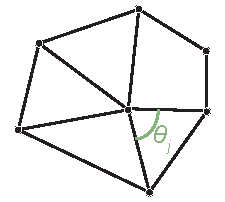
\includegraphics{images/PointIncidentAngles}
\hfill~

\noindent
We want a worklet to compute $\sum_{j} \theta$ for all such attached angles.
This measure is related (but not the same as) the curvature of the surface.
A flat surface will have a sum of $2\pi$.
Convex and concave surfaces have a value less than $2\pi$, and saddle surfaces have a value greater than $2\pi$.

To do this, we create a map cell to point worklet (Section~\ref{sec:WorkletMapCellToPoint}) that visits every point and gives the index of every incident cell.
The worklet then uses a whole cell set to inspect each incident cell to measure the attached angle and sum them together.

\vtkmlisting{Using \protect\sigtag{WholeCellSetIn} to sum the angles around each point.}{SumOfAngles.cxx}

\index{control~signature!whole cell set|)}
\index{worklet!whole cell set|)}
\index{cell~set!whole|)}
\index{whole cell set|)}

\section{Execution Objects}
\label{sec:ExecutionObjects}

\index{execution~object|(}
\index{worklet!execution~object|(}
\index{control~signature!execution~object|(}

Although passing whole arrays and cell sets into a worklet is a convenient way to provide data to a worklet that is not divided by the input or output domain, they is sometimes not the best structures to represent data.
Thus, all worklets support a another type of argument called an \keyterm{execution object}, or exec object for short, that passes the given object directly to each invocation of the worklet.
This is defined by an \sigtag{ExecObject} tag in the \controlsignature.

The execution object must be a subclass of \vtkmexec{ExecutionObjectBase}.
Also, it must be possible to copy the object from the control environment
to the execution environment and be usable in the execution environment,
and any method of the execution object used within the worklet must be
declared with \vtkmexecmodifier or \vtkmexeccontmodifier.

An execution object can refer to an array, but the array reference must be
through an array portal for the execution environment. This can be
retrieved from the \textcode{PrepareForInput} method in
\vtkmcont{ArrayHandle} as described in
Section~\ref{sec:ArrayHandle:InterfaceToExecutionEnvironment}. Other VTK-m
data objects, such as the subclasses of \vtkmcont{CellSet}, have similar
methods.

Returning to the example we have in Section~\ref{sec:WholeArrays}, we are
computing triangle quality quickly by looking up the value in a table. In
Example~\ref{ex:TriQualityWholeArray} the table is passed directly to the
worklet as a whole array. However, there is some additional code involved
to get the appropriate index into the table for a given triangle. Let us
say that we want to have the ability to compute triangle quality in many
different worklets. Rather than pass in a raw array, it would be better to
encapsulate the functionality in an object.

We can do that by creating an execution object that has the table stored
inside and methods to compute the triangle quality. The following example
uses the table built in Example~\ref{ex:TriQualityWholeArray} to create
such an object.

\vtkmlisting[ex:TriQualityExecObject]{Using \protect\sigtag{ExecObject} to access a lookup table in a worklet.}{TriangleQualityExecObject.cxx}

\index{control~signature!execution~object|)}
\index{worklet!execution~object|)}
\index{execution~object|)}

\section{Scatter}
\label{sec:WorkletScatter}

\index{scatter|(}
\index{worklet!scatter|(}

The default scheduling of a worklet provides a 1 to 1 mapping from the
input domain to the output domain. For example, a
\vtkmworklet{WorkletMapField} gets run once for every item of the input
array and produces one item for the output array. Likewise,
\vtkmworklet{WorkletMapPointToCell} gets run once for every cell in the
input topology and produces one associated item for the output field.

However, there are many operations that do not fall well into this 1 to 1
mapping procedure. The operation might need to pass over elements that
produce no value or the operation might need to produce multiple values for
a single input element.

Such non 1 to 1 mappings can be achieved by defining a \keyterm{scatter}
for a worklet. The following types of scatter are provided by VTK-m.

\begin{description}
\item[\vtkmworklet{ScatterIdentity}] Provides a basic 1 to 1 mapping from
  input to output. This is the default scatter used if none is specified.
\item[\vtkmworklet{ScatterUniform}] Provides a 1 to many mapping from input
  to output with the same number of outputs for each input. The worklet
  provides a number at runtime that defines the number of output values to
  produce per input.
\item[\vtkmworklet{ScatterCounting}] Provides a 1 to any mapping from input
  to output with different numbers of outputs for each input. The worklet
  provides an \textidentifier{ArrayHandle} that is the same size as the
  input containing the count of output values to produce for each input.
  Values can be zero, in which case that input will be skipped.
\end{description}

To define a scatter procedure, the worklet must provide two items. The
first item is a type definition named \scattertype. The \scattertype
must be set to one of the aforementioned
\textidentifier{Scatter*} classes. The second item is a \textcode{const}
method named \textcode{GetScatter} that returns an object of type
\scattertype.

\vtkmlisting{Declaration of a scatter type in a worklet.}{DeclareScatter.cxx}

When using a scatter that produces multiple outputs for a single input, the worklet is invoked multiple times with the same input values.
In such an event the worklet operator needs to distinguish these calls to produce the correct associated output.
This is done by declaring one of the \executionsignature arguments as \index{visit~index} \sigtag{VisitIndex}.
This tag will pass a \vtkm{IdComponent} to the worklet that identifies which invocation is being called.

It is also the case that the when a scatter can produce multiple outputs for some input that the index of the input element is not the same as the \sigtag{WorkIndex}.
If the index to the input element is needed, you can use the \index{input index} \sigtag{InputIndex} tag in the \executionsignature.
It is also good practice to use the \index{output index} \sigtag{OutputIndex} tag if the index to the output element is needed.

To demonstrate using scatters with worklets, we provide some contrived but
illustrative examples. The first example is a worklet that takes a pair of
input arrays and interleaves them so that the first, third, fifth, and so
on entries come from the first array and the second, fourth, sixth, and so
on entries come from the second array. We achieve this by using a
\vtkmcont{ScatterUniform} of size 2 and using the \sigtag{VisitIndex} to
determine from which array to pull a value.

\vtkmlisting{Using \textidentifier{ScatterUniform}.}{ScatterUniform.cxx}

The second example takes a collection of point coordinates and clips them
by an axis-aligned bounding box. It does this using a
\vtkmcont{ScatterCounting} with an array containing 0 for all points
outside the bounds and 1 for all points inside the bounds. As is typical
with this type of operation, we use another worklet with a default identity
scatter to build the count array.

\vtkmlisting{Using \textidentifier{ScatterCounting}.}{ScatterCounting.cxx}

\index{worklet!scatter|)}
\index{scatter|)}


\section{Error Handling}
\label{sec:ExecutionEnvironment:ErrorHandling}
\label{sec:Worklet:ErrorHandling}

\index{errors|(}

\index{errors!execution~environment|(}
\index{errors!worklet|(}
\index{worklet!error~handling|(}

It is sometimes the case during the execution of an algorithm that an error
condition can occur that causes the computation to become invalid. At such
a time, it is important to raise an error to alert the calling code of the
problem. Since VTK-m uses an exception mechanism to raise errors, we want
an error in the execution environment to throw an exception.

However, throwing exceptions in a parallel algorithm is problematic. Some
accelerator architectures, like CUDA, do not even support throwing
exceptions. Even on architectures that do support exceptions, throwing them
in a thread block can cause problems. An exception raised in one thread may
or may not be thrown in another, which increases the potential for
deadlocks, and it is unclear how uncaught exceptions progress through
thread blocks.

VTK-m handles this problem by using a flag and check mechanism. When a
worklet (or other subclass of \vtkmexec{FunctorBase}) encounters an error,
it can call its \textcode{RaiseError} method to flag the problem and record
a message for the error. Once all the threads terminate, the scheduler
checks for the error, and if one exists it throws a
\vtkmcont{ErrorExecution} exception in the control environment. Thus,
calling \textcode{RaiseError} looks like an exception was thrown from the
perspective of the control environment code that invoked it.

\vtkmlisting{Raising an error in the execution environment.}{ExecutionErrors.cxx}

\index{worklet!error~handling|)}
\index{errors!worklet|)}
\index{errors!execution~environment|)}

\index{errors!assert|(}
\index{assert|(}

It is also worth noting that the \vtkmmacro{VTKM\_ASSERT} macro described
in Section~\ref{sec:ErrorHandlingControl} also works within worklets and
other code running in the execution environment. Of course, a failed assert
will terminate execution rather than just raise an error so is best for
checking invalid conditions for debugging purposes.

\index{assert|)}
\index{errors!assert|)}

\index{errors|)}

\index{worklet!creating|)}
\index{worklet|)}


  % -*- latex -*-

\chapter{Creating Filters}
\label{chap:CreatingFilters}

\index{filter|(}

In Chapter~\ref{chap:Worklets} we discuss how to implement an algorithm in the VTK-m framework by creating a worklet.
Worklets might be straightforward to implement and invoke for those well familiar with the appropriate VTK-m API.
However, novice users have difficulty using worklets directly.
For simplicity, worklet algorithms are generally wrapped in what are called filter objects for general usage.
Chapter~\ref{chap:ProvidedFilters} introduces the concept of filters and documents those that come with the VTK-m library.
In this chapter we describe how to build new filter objects using the worklet examples introduced in Chapter~\ref{chap:Worklets}.

Unsurprisingly, the base filter objects are contained in the \vtkmfilter{} package.
The basic implementation of a filter involves subclassing one of the base filter objects and implementing the \textcode{DoExecute} method.
The \textcode{DoExecute} method performs the operation of the filter and returns the appropriate result object.

As with worklets, there are several flavors of filter types to address different operating behaviors although their is not a one-to-one relationship between worklet and filter types.
This chapter is sectioned by the different filter types with an example of implementations for each.

\section{Field Filters}

\index{filter!field|(}
\index{field filter|(}

As described in Section~\ref{sec:ProvidedFieldFilters} (starting on page~\pageref{sec:ProvidedFieldFilters}), field filters are a category of filters that generate a new fields.
These new fields are typically derived from one or more existing fields or point coordinates on the data set.
For example, mass, volume, and density are interrelated, and any one can be derived from the other two.

Field filters are implemented in classes that derive the \vtkmfilter{FilterField} base class.
\textidentifier{FilterField} is a templated class that has a single template argument, which is the type of the concrete subclass.

\begin{didyouknow}
  The convention of having a subclass be templated on the derived class' type is known as the Curiously Recurring Template Pattern (CRTP).
  In the case of \textidentifier{FilterField} and other filter base classes, \VTKm uses this CRTP behavior to allow the general implementation of these algorithms to run \textcode{DoExecute} in the subclass, which as we see in a moment is itself templated.
\end{didyouknow}

All \textidentifier{FilterField} subclasses must implement a \textcode{DoExecute} method.
The \textidentifier{FilterField} base class implements an \textcode{Execute} method (actually several overloaded versions of \textcode{Execute}), processes the arguments, and then calls the \textcode{DoExecute} method of its subclass.
The \textcode{DoExecute} method has the following 5 arguments.
\begin{itemize}
\item
  An input data set contained in a \vtkmcont{DataSet} object.
  (See Chapter~\ref{chap:DataSet} for details on \textidentifier{DataSet} objects.)
\item
  The field from the \textidentifier{DataSet} specified in the \textcode{Execute} method to operate on.
  The field is always passed as an instance of \vtkmcont{ArrayHandle}.
  (See Chapter~\ref{chap:ArrayHandle} for details on \textidentifier{ArrayHandle} objects.)
  The type of the \textidentifier{ArrayHandle} is generally not known until the class is used and requires a template type.
\item
  A \vtkmfilter{FieldMetadata} object that contains the associated metadata of the field not contained in the \textidentifier{ArrayHandle} of the second argument.
  The \textidentifier{FieldMetadata} contains information like the name of the field and what topological element the field is associated with (such as points or cells).
\item
  A policy class.
  (See Chapter~\ref{chap:Policies} for details on policy classes.)
  The type of the policy is generally to known until the class is used and requires a template type.
\item
  A device adapter tag.
  (See Chapter~\ref{chap:DeviceAdapter} for details on device adapters and their tags.)
  The type of the device adapter is generally to known until the class is used and requires a template type.
\end{itemize}

In this section we provide an example implementation of a field filter that wraps the ``magnitude'' worklet provided in Example~\ref{ex:UseWorkletMapField} (listed on page~\pageref{ex:UseWorkletMapField}).
By convention, filter implementations are split into two files.
The first file is a standard header file with a \textfilename{.h} extension that contains the declaration of the filter class without the implementation.
So we would expect the following code to be in a file named \textfilename{FieldMagnitude.h}.

\vtkmlisting[ex:MagnitudeFilterDeclaration]{Header declaration for a field filter.}{UseFilterField.cxx}

\index{filter!traits|(}
\index{traits!filter|(}

Notice that in addition to declaring the class for \textcode{FieldMagnitude}, Example~\ref{ex:MagnitudeFilterDeclaration} also specializes the \vtkmfilter{FilterTraits} templated class for \textcode{FieldMagnitude}.
The \textidentifier{FilterTraits} class, declared in \vtkmheader{vtkm/filter}{FilterTraits.h}, provides hints used internally in the base filter classes to modify its behavior based on the subclass.
A \textidentifier{FilterTraits} class is expected to define the following types.
\begin{description}
\item[\textcode{InputFieldTypeList}]
  A type list containing all the types that are valid for the input field.
  For example, a filter operating on positions in space might limit the types to three dimensional vectors.
  Type lists are discussed in detail in Section~\ref{sec:TypeLists}.
\end{description}

In the particular case of our \textcode{FieldMagnitude} filter, the filter expects to operate on some type of vector field.
Thus, the \textcode{InputFieldTypeList} is modified to a list of all standard floating point \textidentifier{Vec}s.

Once the filter class and (optionally) the \textidentifier{FilterTraits} are declared in the \textfilename{.h} file, the implementation filter is by convention given in a separate \textfilename{.hxx} file.
So the continuation of our example that follows would be expected in a file named \textfilename{FieldMagnitude.hxx}.
The \textfilename{.h} file near its bottom needs an include line to the \textfilename{.hxx} file.
This convention is set up because a near future version of \VTKm will allow the building of filter libraries containing default policies that can be used by only including the header declaration.

The implementation of \textcode{DoExecute} is straightforward.
A worklet is invoked to compute a new field array.
\textcode{DoExecute} then returns a newly constructed \vtkmfilter{ResultField} object.
The constructor to \textidentifier{ResultField} takes the following 5 arguments.
\begin{itemize}
\item
  The input data set.
  This is the same data set passed to the first argument of \textcode{DoExecute}.
\item
  The array containing the data for the new field, which was presumably computed by the filter.
\item
  The name of the new field.
\item
  The topological association (e.g. points or cells) of the new field.
  In the case where the filter is a simple operation on a field array, the association can usually be copied from the \textidentifier{FieldMetadata} passed to \textcode{DoExecute}.
\item
  The name of the element set the new field is associated with.
  This only has meaning if the new field is associated with cells.
  This usually can be copied from the \textidentifier{FieldMetadata} passed to \textcode{DoExecute}.
\end{itemize}

Note that all fields need a unique name, which is the reason for the third argument to the \textidentifier{ResultField} constructor.
The \vtkmfilter{FilterField} base class contains a pair of methods named \textcode{SetOutputFieldName} and \textcode{GetOutputFieldName} to allow users to specify the name of output fields.
The \textcode{DoExecute} method should respect the given output field name.
However, it is also good practice for the filter to have a default name if none is given.
This might be simply specifying a name in the constructor, but it is worthwhile for many filters to derive a name based on the name of the input field.

\vtkmlisting{Implementation of a field filter.}{FilterFieldImpl.cxx}

\index{traits!filter|)}
\index{filter!traits|)}

\index{field filter|)}
\index{filter!field|)}

\index{filter|)}


  % -*- latex -*-

\chapter{Math}
\label{chap:Math}

\index{math|(}

VTK-m comes with several math functions that tend to be useful for
visualization algorithms. The implementation of basic math operations can
vary subtly on different accelerators, and these functions provide cross
platform support.

All math functions are located in the \vtkm{} package. The functions are
most useful in the execution environment, but they can also be used in the
control environment when needed.

\section{Basic Math}

The \vtkmheader{vtkm}{Math.h} header file contains several math functions
that replicate the behavior of the basic POSIX math functions as well as
related functionality.

\begin{didyouknow}
  When writing worklets, you should favor using these math functions
  provided by VTK-m over the standard math functions in
  \textfilename{math.h}. VTK-m's implementation manages several compiling
  and efficiency issues when porting.
\end{didyouknow}

\begin{description}
\item[\vtkm{Abs}] \index{absolute value} Returns the absolute value of
  the single argument. If given a vector, performs a component-wise
  operation.
\item[\vtkm{ACos}] \index{arccosine} \index{inverse cosine} Returns the
  arccosine of a ratio in radians. If given a vector, performs a
  component-wise operation.
\item[\vtkm{ACosH}] \index{hyperbolic arccossine} \index{inverse hyperbolic cosine}
  Returns the hyperbolic arccossine. If given a vector, performs a
  component-wise operation.
\item[\vtkm{ASin}] \index{arcsine} \index{inverse sine} Returns the
  arcsine of a ratio in radians. If given a vector, performs a
  component-wise operation.
\item[\vtkm{ASinH}] \index{hyperbolic arcsine} \index{inverse hyperbolic sine}
  Returns the hyperbolic arcsine. If given a vector, performs a
  component-wise operation.
\item[\vtkm{ATan}] \index{arctangent} \index{inverse tangent} Returns the
  arctangent of a ratio in radians. If given a vector, performs a
  component-wise operation.
\item[\vtkm{ATan2}] Computes the arctangent of $y/x$ where $y$ is the
  first argument and $x$ is the second argument. \textidentifier{ATan2}
  uses the signs of both arguments to determine the quadrant of the return
  value. \textidentifier{ATan2} is only defined for floating point types
  (no vectors).
\item[\vtkm{ATanH}] \index{hyperbolic tangent} \index{inverse hyperbolic tangent}
  Returns the hyperbolic arctangent. If given a vector, performs a
  component-wise operation.
\item[\vtkm{Cbrt}] \index{cube root} Takes one argument and returns the
  cube root of that argument. If called with a vector type, returns a
  component-wise cube root.
\item[\vtkm{Ceil}] \index{ceiling} \index{round up|see{ceiling}} Rounds
  and returns the smallest integer not less than the single argument. If
  given a vector, performs a component-wise operation.
\item[\vtkm{CopySign}] Copies the sign of the second argument onto the
  first argument and returns that. If the second argument is positive,
  returns the absolute value of the first argument. If the second argument
  is negative, returns the negative absolute value of the first argument.
\item[\vtkm{Cos}] \index{cosine} Returns the cosine of an angle given in
  radians. If given a vector, performs a component-wise operation.
\item[\vtkm{CosH}] \index{hyperbolic cosine} Returns the hyperbolic
  cosine. If given a vector, performs a component-wise operation.
\item[\vtkm{Epsilon}] Returns the difference between 1 and the least
  value greater than 1 that is representable by a floating point number.
  Epsilon is useful for specifying the tolerance one should have when
  considering numerical error. The \textidentifier{Epsilon} method is
  templated to specify either a 32 or 64 bit floating point number. The
  convenience methods \textidentifier{Epsilon32} and
  \textidentifier{Epsilon64} are non-templated versions that return the
  precision for a particular precision.
\item[\vtkm{Exp}] \index{exponential} Computes $e^x$ where $x$ is the
  argument to the function and $e$ is Euler's number (approximately
  $2.71828$). If called with a vector type, returns a component-wise
  exponent.
\item[\vtkm{Exp10}] Computes $10^x$ where $x$ is the argument. If called
  with a vector type, returns a component-wise exponent.
\item[\vtkm{Exp2}] Computes $2^x$ where $x$ is the argument. If called
  with a vector type, returns a component-wise exponent.
\item[\vtkm{ExpM1}] Computes $e^x-1$ where $x$ is the argument to the
  function and $e$ is Euler's number (approximately $2.71828$). The
  accuracy of this function is good even for very small values of $x$. If
  called with a vector type, returns a component-wise exponent.
\item[\vtkm{Floor}] \index{floor} \index{round down|see{floor}} Rounds
  and returns the largest integer not greater than the single argument. If
  given a vector, performs a component-wise operation.
\item[\vtkm{FMod}] \index{remainder} Computes the remainder on the
  division of 2 floating point numbers. The return value is $numerator - n
  \cdot denominator$, where $numerator$ is the first argument,
  $denominator$ is the second argument, and $n$ is the quotient of
  $numerator$ divided by $denominator$ rounded towards zero to an
  integer. For example, \textidentifier{FMod}\textcode{(6.5,2.3)} returns
  $1.9$, which is $6.5 - 2\cdot4.6$. If given vectors,
  \textidentifier{FMod} performs a component-wise
  operation. \textidentifier{FMod} is similar to \textidentifier{Remainder}
  except that the quotient is rounded toward 0 instead of the nearest
  integer.
\item[\vtkm{Infinity}] Returns the representation for infinity. The result
  is greater than any other number except another infinity or NaN. When
  comparing two infinities or infinity to NaN, neither is greater than,
  less than, nor equal to the other. The \textidentifier{Infinity} method
  is templated to specify either a 32 or 64 bit floating point number. The
  convenience methods \textidentifier{Infinity32} and
  \textidentifier{Infinity64} are non-templated versions that return the
  precision for a particular precision.
\item[\vtkm{IsFinite}] Returns true if the argument is a normal number
  (neither a NaN nor an infinite).
\item[\vtkm{IsInf}] Returns true if the argument is either positive
  infinity or negative infinity.
\item[\vtkm{IsNan}] Returns true if the argument is not a number (NaN).
\item[\vtkm{IsNegative}] \index{negative} Returns true if the single
  argument is less than zero, false otherwise.
\item[\vtkm{Log}] \index{natural logarithm} \index{logarithm} Computes
  the natural logarithm (i.e. logarithm to the base $e$) of the single
  argument. If called with a vector type, returns a component-wise
  logarithm.
\item[\vtkm{Log10}] \index{logarithm} Computes the logarithm to the base
  10 of the single argument. If called with a vector type, returns a
  component-wise logarithm.
\item[\vtkm{Log1P}] \index{natural logarithm} \index{logarithm} Computes
  $\ln(1+x)$ where $x$ is the single argument and $\ln$ is the natural
  logarithm (i.e. logarithm to the base $e$). The accuracy of this function
  is good for very small values. If called with a vector type, returns a
  component-wise logarithm.
\item[\vtkm{Log2}] \index{logarithm} Computes the logarithm to the base
  2 of the single argument. If called with a vector type, returns a
  component-wise logarithm.
\item[\vtkm{Max}] \index{maximum} Takes two arguments and returns the
  argument that is greater. If called with a vector type, returns a
  component-wise maximum.
\item[\vtkm{Min}] \index{minimum} Takes two arguments and returns the
  argument that is lesser. If called with a vector type, returns a
  component-wise minimum.
\item[\vtkm{ModF}] Returns the integral and fractional parts of the
  first argument. The second argument is a reference in which the integral
  part is stored. The return value is the fractional part. If given
  vectors, \textidentifier{ModF} performs a component-wise operation.
\item[\vtkm{Nan}] \index{not a number} Returns the representation for
  not-a-number (NaN). A NaN represents an invalid value or the result of an
  invalid operation such as $0/0$. A NaN is neither greater than nor less
  than nor equal to any other number including other NaNs. The
  \textidentifier{NaN} method is templated to specify either a 32 or 64 bit
  floating point number. The convenience methods \textidentifier{Nan32} and
  \textidentifier{NaN64} are non-templated versions that return the
  precision for a particular precision.
\item[\vtkm{NegativeInfinity}] Returns the representation for negative
  infinity. The result is less than any other number except another
  negative infinity or NaN. When comparing two negative infinities or
  negative infinity to NaN, neither is greater than, less than, nor equal
  to the other. The \textidentifier{NegativeInfinity} method is templated
  to specify either a 32 or 64 bit floating point number. The convenience
  methods \textidentifier{NagativeInfinity32} and
  \textidentifier{NegativeInfinity64} are non-templated versions that
  return the precision for a particular precision.
\item[\vtkm{Pi}] \index{$\pi$} Returns the constant $\pi$ (about
  $3.14159$).
\item[\vtkm{Pi\_2}] \index{$\pi$} Returns the constant $\pi/2$ (about
  $1.570796$).
\item[\vtkm{Pi\_3}] \index{$\pi$} Returns the constant $\pi/3$ (about
  $1.047197$).
\item[\vtkm{Pi\_4}] \index{$\pi$} Returns the constant $\pi/4$ (about
  $0.785398$).
\item[\vtkm{Pow}] \index{power} Takes two arguments and returns the
  first argument raised to the power of the second argument. This function
  is only defined for \vtkm{Float32} and \vtkm{Float64}.
\item[\vtkm{RCbrt}] \index{reciprocal cube root} Takes one argument and
  returns the cube root of that argument. The result of this function is
  equivalent to \textcode{1/Cbrt(x)}. However, on some devices it is faster
  to compute the reciprocal cube root than the regular cube root. Thus, you
  should use this function whenever dividing by the cube root.
\item[\vtkm{Remainder}] \index{remainder} Computes the remainder on the
  division of 2 floating point numbers. The return value is $numerator - n
  \cdot denominator$, where $numerator$ is the first argument,
  $denominator$ is the second argument, and $n$ is the quotient of
  $numerator$ divided by $denominator$ rounded towards the nearest
  integer. For example, \textidentifier{FMod}\textcode{(6.5,2.3)} returns
  $-0.4$, which is $6.5 - 3\cdot2.3$. If given vectors,
  \textidentifier{Remainder} performs a component-wise
  operation. \textidentifier{Remainder} is similar to \textidentifier{FMod}
  except that the quotient is rounded toward the nearest integer instead of
  toward 0.
\item[\vtkm{RemainderQuotient}] Performs an operation identical to
  \textidentifier{Reminder}. In addition, this function takes a third
  argument that is a reference in which the quotient is given.
\item[\vtkm{Round}] Rounds and returns the integer nearest the single
  argument. If given a vector, performs a component-wise operation.
\item[\vtkm{RSqrt}] \index{reciprocal square root} Takes one argument
  and returns the square root of that argument. The result of this function
  is equivalent to \textcode{1/Sqrt(x)}. However, on some devices it is
  faster to compute the reciprocal square root than the regular square
  root. Thus, you should use this function whenever dividing by the square
  root.
\item[\vtkm{SignBit}] Returns a nonzero value if the single argument is
  negative.
\item[\vtkm{Sin}] \index{sine} Returns the sine of an angle given in
  radians. If given a vector, performs a component-wise operation.
\item[\vtkm{SinH}] \index{hyperbolic sine} Returns the hyperbolic
  sine. If given a vector, performs a component-wise operation.
\item[\vtkm{Sqrt}] \index{square root} Takes one argument and returns
  the square root of that argument. If called with a vector type, returns a
  component-wise square root. On some hardware it is faster to find the
  reciprocal square root, so \textidentifier{RSqrt} should be used if you
  actually plan to divide byt the square root.
\item[\vtkm{Tan}] \index{tangent} Returns the tangent of an angle given
  in radians. If given a vector, performs a component-wise operation.
\item[\vtkm{TanH}] \index{hyperbolic tangent} Returns the hyperbolic
  tangent. If given a vector, performs a component-wise operation.
\item[\vtkm{TwoPi}] \index{$\pi$} Returns the constant $2\pi$ (about
  $6.283185$).
\end{description}

\section{Vector Analysis}

\index{vector~analysis|(}

Visualization and computational geometry algorithms often perform vector
analysis operations. The \vtkmheader{vtkm}{VectorAnalysis.h} header file
provides functions that perform the basic common vector analysis
operations.

\begin{description}
\item[\vtkm{Cross}] \index{cross product} Returns the cross product of
  two \vtkm{Vec} of size 3.
\item[\vtkm{Lerp}] \index{linear interpolation} Given two values $x$ and
  $y$ in the first two parameters and a weight $w$ as the third parameter,
  interpolates between $x$ and $y$. Specifically, the linear interpolation
  is $(y-x)w + x$ although \textidentifier{Lerp} might compute the
  interpolation faster than using the independent arithmetic operations.
  The two values may be scalars or equal sized vectors. If the two values
  are vectors and the weight is a scalar, all components of the vector are
  interpolated with the same weight. If the weight is also a vector, then
  each component of the value vectors are interpolated with the respective
  weight component.
\item[\vtkm{Magnitude}] Returns the magnitude of a vector. This function
  works on scalars as well as vectors, in which case it just returns the
  scalar. It is usually much faster to compute
  \textidentifier{MagnitudeSquared}, so that should be substituted when
  possible (unless you are just going to take the square root, which would
  be besides the point). On some hardware it is also faster to find the
  reciprocal magnitude, so \textidentifier{RMagnitude} should be used if
  you actually plan to divide by the magnitude.
\item[\vtkm{MagnitudeSquared}] Returns the square of the magnitude of a
  vector. It is usually much faster to compute the square of the magnitude
  than the length, so you should use this function in place of
  \textidentifier{Magnitude} or \textidentifier{RMagnitude} when needing
  the square of the magnitude or any monotonically increasing function of a
  magnitude or distance. This function works on scalars as well as vectors,
  in which case it just returns the square of the scalar.
\item[\vtkm{Normal}] Returns a normalized version of the given
  vector. The resulting vector points in the same direction as the argument
  but has unit length.
\item[\vtkm{Normalize}] Takes a reference to a vector and modifies it to
  be of unit length. \textidentifier{Normalize}\textcode{(v)} is
  functionally equivalent to
  \textcode{v *= }\textidentifier{RMagnitude}\textcode{(v)}.
\item[\vtkm{RMagnitude}] Returns the reciprocal magnitude of a
  vector. On some hardware \textidentifier{RMagnitude} is faster than
  \textidentifier{Magnitude}, but neither is as fast as
  \textidentifier{MagnitudeSquared}. This function works on scalars as well
  as vectors, in which case it just returns the reciprocal of the scalar.
\item[\vtkm{TriangleNormal}] Given three points in space (contained in
  \vtkm{Vec}s of size 3) that compose a triangle return a vector that is
  perpendicular to the triangle. The magnitude of the result is equal to
  twice the area of the triangle. The result points away from the ``front''
  of the triangle as defined by the standard counter-clockwise ordering of
  the points.
\end{description}

\index{vector~analysis|)}

\section{Matrices}
\label{sec:Math:Matrices}

\index{matrix|(}

Linear algebra operations on small matrices that are done on a single
thread are located in \vtkmheader{vtkm}{Matrix.h}.

This header defines the \vtkm{Matrix} templated class. The template
parameters are first the type of component, then the number of rows, then
the number of columns. The overloaded parentheses operator can be used to
retrieve values based on row and column indices. Likewise, the bracket
operators can be used to reference the \textidentifier{Matrix} as a 2D
array (indexed by row first). The following example builds a
\textidentifier{Matrix} that contains the values
\begin{equation*}
  \left|
  \begin{array}{ccc}
    0 & 1 & 2 \\
    10 & 11 & 12
  \end{array}
  \right|
\end{equation*}

\vtkmlisting{Creating a \textidentifier{Matrix}.}{BuildMatrix.cxx}

The \vtkmheader{vtkm}{Matrix.h} header also defines the following functions
that operate on matrices.

\begin{description}
\item[\vtkm{MatrixDeterminant}] \index{determinant} Takes a square
  \textidentifier{Matrix} as its single argument and returns the
  determinant of that matrix.
\item[\vtkm{MatrixGetColumn}] \index{column} Given a
  \textidentifier{Matrix} and a column index, returns a \vtkm{Vec} of that
  column. This function might not be as efficient as \vtkm{MatrixRow}. (It
  performs a copy of the column).
\item[\vtkm{MatrixGetRow}] \index{row} Given a \textidentifier{Matrix} and
  a row index, returns a \vtkm{Vec} of that row.
\item[\vtkm{MatrixIdentity}] \index{identity matrix} Returns the
  identity matrix. If given no arguments, it creates an identity matrix and
  returns it. (In this form, the component type and size must be explicitly
  set.) If given a single square matrix argument, fills that matrix with
  the identity.
\item[\vtkm{MatrixInverse}] \index{inverse matrix} Finds and returns the
  inverse of a given matrix. The function takes two arguments. The first
  argument is the matrix to invert. The second argument is a reference to a
  Boolean that is set to true if the inverse is found or false if the
  matrix is singular and the returned matrix is incorrect.
\item[\vtkm{MatrixMultiply}] Performs a matrix-multiply on its two
  arguments. Overloaded to work for matrix-matrix, vector-matrix, or
  matrix-vector multiply.
\item[\vtkm{MatrixSetColumn}] Given a \textidentifier{Matrix}, a column
  index, and a \vtkm{Vec}, sets the column of that index to the values of
  the \textidentifier{Tuple}.
\item[\vtkm{MatrixSetRow}] Given a \textidentifier{Matrix}, a row index,
  and a \vtkm{Vec}, sets the row of that index to the values of the
  \textidentifier{Tuple}.
\item[\vtkm{MatrixTranspose}] \index{transpose matrix} Takes a
  \textidentifier{Matrix} and returns its transpose.
\item[\vtkm{SolveLinearSystem}] \index{linear system} Solves the linear
  system $\matrixsym{A}\vectorsym{x} = \vectorsym{b}$ and returns
  $\vectorsym{x}$. The function takes three arguments. The first two
  arguments are the matrix $\matrixsym{A}$ and the vector $\vectorsym{b}$,
  respectively. The third argument is a reference to a Boolean that is set
  to true if a single solution is found, false otherwise.
\end{description}

\index{matrix|)}

\section{Newton's Method}

\index{Newton's method|(}

VTK-m's matrix methods (documented in Section~\ref{sec:Math:Matrices})
provide a method to solve a small linear system of equations. However,
sometimes it is necessary to solve a small nonlinear system of equations.
This can be done with the \vtkm{NewtonsMethod} function defined in the
\vtkmheader{vtkm}{NewtonsMethod.h} header.

The \textidentifier{NewtonsMethod} function assumes that the number of
variables equals the number of equations. Newton's method operates on an
iterative evaluate and search. Evaluations are performed using the functors
passed into the \textidentifier{NewtonsMethod}. The function takes the
following 6 parameters (three of which are optional).

\begin{enumerate}
\item A functor whose operation takes a \vtkm{Vec} and returns a
  \vtkm{Matrix} containing the math function's Jacobian vector at that
  point.
\item A functor whose operation takes a \vtkm{Vec} and returns the
  evaluation of the math function at that point as another \vtkm{Vec}.
\item The \vtkm{Vec} that represents the desired output of the function.
\item A \vtkm{Vec} to use as the initial guess. If not specified, the
  origin is used.
\item The convergence distance. If the iterative method changes all
  values less than this amount, then it considers the solution found. If
  not specified, set to $10^{-3}$.
\item The maximum amount of iterations to run before giving up and
  returning the best solution. If not specified, set to $10$.
\end{enumerate}

\vtkmlisting{Using \textidentifier{NewtonsMethod} to solve a small system of nonlinear equations.}{NewtonsMethod.cxx}

\index{Newton's method|)}

\index{math|)}


  % -*- latex -*-

\chapter{Working with Cells}
\label{chap:WorkingWithCells}

In the control environment, data is defined in mesh structures that
comprise a set of finite cells. (See Section~\ref{sec:DataSets:CellSets}
starting on page~\pageref{sec:DataSets:CellSets} for information on
defining cell sets in the control environment.) When worklets that operate
on cells are scheduled, these grid structures are broken into their
independent cells, and that data is handed to the worklet. Thus, cell-based
operations in the execution environment exclusively operate on independent
cells.

Unlike some other libraries such as VTK, VTK-m does not have a cell class
that holds all the information pertaining to a cell of a particular type.
Instead, VTK-m provides tags or identifiers defining the cell shape, and
companion data like coordinate and field information are held in separate
structures. This organization is designed so a worklet may specify exactly
what information it needs, and only that information will be loaded.

\section{Cell Shape Tags and Ids}
\label{sec:CellShapeTagsIds}

\index{shape|(}
\index{cell~shape|(}
\index{tag!cell~shape|(}
\index{tag!shape|(}

Cell shapes can be specified with either a tag (defined with a struct with
a name like \textidentifier{CellShapeTag*}) or an enumerated identifier
(defined with a constant number with a name like
\textidentifier{CELL\_SHAPE\_*}). These shape tags and identifiers are
defined in \vtkmheader{vtkm}{CellShape.h} and declared in the \vtkm{}
namespace (because they can be used in either the control or the execution
environment). Figure~\ref{fig:CellShapes} gives both the identifier and the
tag names.

\begin{figure}
  \centering
  \small
  \begin{tabular}{@{}c@{~}c@{~}c@{}}
    \raisebox{-0.5\height}{
\includegraphics{images/CellConnectionsVertex}} &
    \raisebox{-0.5\height}{
\includegraphics{images/CellConnectionsLine}} &
    \raisebox{-0.5\height}{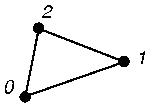
\includegraphics{images/CellConnectionsTriangle}} \\
    \vtkm{CELL\_SHAPE\_VERTEX} &
    \vtkm{CELL\_SHAPE\_LINE} &
    \vtkm{CELL\_SHAPE\_TRIANGLE} \\
    \vtkm{CellShapeTagVertex} \index{vertex} &
    \vtkm{CellShapeTagLine} \index{line} &
    \vtkm{CellShapeTagTriangle} \index{triangle} \\[2ex]
    \raisebox{-0.5\height}{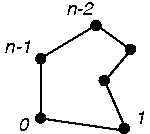
\includegraphics{images/CellConnectionsPolygon}} &
    \raisebox{-0.5\height}{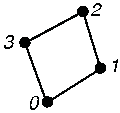
\includegraphics{images/CellConnectionsQuadrilateral}} &
    \raisebox{-0.5\height}{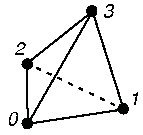
\includegraphics{images/CellConnectionsTetrahedron}} \\
    \vtkm{CELL\_SHAPE\_POLYGON} &
    \vtkm{CELL\_SHAPE\_QUAD} &
    \vtkm{CELL\_SHAPE\_TETRA} \\
    \vtkm{CellShapeTagPolygon} \index{polygon} &
    \vtkm{CellShapeTagQuad} \index{quadrilateral} &
    \vtkm{CellShapeTagTetra} \index{tetrahedron} \\[2ex]
    \raisebox{-0.5\height}{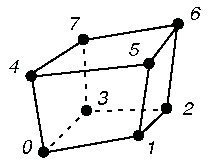
\includegraphics{images/CellConnectionsHexahedron}} &
    \raisebox{-0.5\height}{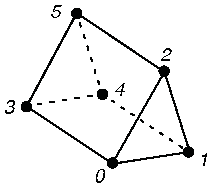
\includegraphics{images/CellConnectionsWedge}} &
    \raisebox{-0.5\height}{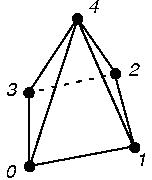
\includegraphics{images/CellConnectionsPyramid}} \\
    \vtkm{CELL\_SHAPE\_HEXAHEDRON} &
    \vtkm{CELL\_SHAPE\_WEDGE} &
    \vtkm{CELL\_SHAPE\_PYRAMID} \\
    \vtkm{CellShapeTagHexahedron} \index{hexahedron} &
    \vtkm{CellShapeTagWedge} \index{wedge} &
    \vtkm{CellShapeTagPyramid} \index{pyramid}
  \end{tabular}
  \caption{Basic Cell Shapes}
  \label{fig:CellShapes}
\end{figure}

In addition to the basic cell shapes, there is a special ``empty'' cell
with the identifier \vtkm{CELL\_SHAPE\_EMPTY} and tag
\vtkm{CellShapeTagEmpty}. This type of cell has no points, edges, or faces
and can be thought of as a placeholder for a null or void cell.

There is also a special cell shape ``tag'' named \vtkm{CellShapeTagGeneric}
that is used when the actual cell shape is not known at compile time.
\textidentifier{CellShapeTagGeneric} actually has a member variable named
\textcode{Id} that stores the identifier for the cell shape. There is no
equivalent identifier for a generic cell; cell shape identifiers can be
placed in a \vtkm{IdComponent} at runtime.

When using cell shapes in templated classes and functions, you can use the
\vtkmmacro{VTKM\_IS\_CELL\_SHAPE\_TAG} to ensure a type is a valid cell
shape tag. This macro takes one argument and will produce a compile error
if the argument is not a cell shape tag type.

\subsection{Converting Between Tags and Identifiers}

Every cell shape tag has a member variable named \textcode{Id} that
contains the identifier for the cell shape. This provides a convenient
mechanism for converting a cell shape tag to an identifier. Most cell shape
tags have their \textcode{Id} member as a compile-time constant, but
\textidentifier{CellShapeTagGeneric} is set at run time.

\vtkmheader{vtkm}{CellShape.h} also declares a templated class named
\vtkm{CellShapeIdToTag} that converts a cell shape identifier to a cell
shape tag. \textidentifier{CellShapeIdToTag} has a single template argument
that is the identifier. Inside the class is a type named \textcode{Tag}
that is the type of the correct tag.

\vtkmlisting{Using \textidentifier{CellShapeIdToTag}.}{CellShapeIdToTag.cxx}

However, \textidentifier{CellShapeIdToTag} is only viable if the identifier
can be resolved at compile time. In the case where a cell identifier is
stored in a variable or an array or the code is using a
\textidentifier{CellShapeTagGeneric}, the correct cell shape is not known
at run time. In this case, \vtkmmacro{vtkmGenericCellShapeMacro} can be
used to check all possible conditions. This macro is embedded in a switch
statement where the condition is the cell shape identifier.
\vtkmmacro{vtkmGenericCellShapeMacro} has a single argument, which is an
expression to be executed. Before the expression is executed, a type named
\textcode{CellShapeTag} is defined as the type of the appropriate cell
shape tag. Often this method is used to implement the condition for a
\textidentifier{CellShapeTagGeneric} in a function overloaded for cell
types. A demonstration of \vtkmmacro{vtkmGenericCellShapeMacro} is given in
Example~\ref{ex:GenericCellNormal}.

\index{tag!shape|)}
\index{tag!cell~shape|)}

\subsection{Cell Traits}

\index{cell~traits|(}

The \vtkmheader{vtkm}{CellTraits.h} header file contains a traits class
named \vtkm{CellTraits} that provides information about a cell. Each
specialization of \textidentifier{CellTraits} contains the following
members.

\begin{description}
\item[\textcode{TOPOLOGICAL\_DIMENSIONS}] Defines the topological
  dimensions of the cell type. This is 3 for polyhedra, 2 for polygons, 1
  for lines, and 0 for points.
\item[\textcode{TopologicalDimensionsTag}] A type set to either
  \vtkm{CellTopologicalDimensionsTag}\textcode{<3>},
  \textidentifier{CellTopologicalDimensionsTag}\textcode{<2>},
  \textidentifier{CellTopologicalDimensionsTag}\textcode{<1>}, or
  \textidentifier{CellTopologicalDimensionsTag}\textcode{<0>}. The number
  is consistent with \textcode{TOPOLOGICAL\_DIMENSIONS}. This tag is
  provided for convenience when specializing functions.
\item[\textcode{IsSizeFixed}] Set to either \vtkm{CellTraitsTagSizeFixed}
  for cell types with a fixed number of points (for example, triangle) or
  \vtkm{CellTraitsTagSizeVariable} for cell types with a variable number of
  points (for example, polygon).
\item[\textcode{NUM\_POINTS}] A \vtkm{IdComponent} set to the number of
  points in the cell. This member is only defined when there is a constant
  number of points (i.e. \textcode{IsSizeFixed} is set to
  \vtkm{CellTraitsTagSizeFixed}).
\end{description}

\vtkmlisting[ex:GenericCellNormal]{Using \textidentifier{CellTraits} to implement a polygon normal estimator.}{GenericCellNormal.cxx}

\index{cell~traits|)}

\index{cell~shape|)}
\index{shape|)}

\section{Parametric and World Coordinates}

\index{parametric~coordinates|(}
\index{world~coordinates|(}
\index{cell!parametric~coordinates|(}
\index{cell!world~coordinates|(}

Each cell type supports a one-to-one mapping between a set of parametric
coordinates in the unit cube (or some subset of it) and the points in 3D
space that are the locus contained in the cell. Parametric coordinates are
useful because certain features of the cell, such as vertex location and
center, are at a consistent location in parametric space irrespective of
the location and distortion of the cell in world space. Also, many field
operations are much easier with parametric coordinates.

The \vtkmheader{vtkm/exec}{ParametricCoordinates.h} header file contains the
following functions for working with parametric coordinates.

\begin{description}
\item[\vtkmexec{ParametricCoordinatesCenter}] Returns the parametric
  coordinates for the center of a given shape. It takes 4 arguments: the
  number of points in the cell, a \vtkm{Vec} of size 3 to store the
  results, a shape tag, and a worklet object (for raising errors). A second
  form of this method takes 3 arguments and returns the result as a
  \vtkm{Vec}\textcode{<}\vtkm{FloatDefault}\textcode{,3>} instead of
  passing it as a parameter.
\item[\vtkmexec{ParametricCoordinatesPoint}] Returns the parametric
  coordinates for a given point of a given shape. It takes 5 arguments: the
  number of points in the cell, the index of the point to query, a
  \vtkm{Vec} of size 3 to store the results, a shape tag, and a worklet
  object (for raising errors). A second form of this method takes 3
  arguments and returns the result as a
  \vtkm{Vec}\textcode{<}\vtkm{FloatDefault}\textcode{,3>} instead of
  passing it as a parameter.
\item[\vtkmexec{ParametricCoordinatesToWorldCoordinates}] Given a vector of
  point coordinates (usually given by a \sigtag{FieldPointIn} worklet
  argument), a \vtkm{Vec} of size 3 containing parametric coordinates, a
  shape tag, and a worklet object (for raising errors), returns the world
  coordinates.
\item[\vtkmexec{WorldCoordinatesToParametricCoordinates}] Given a vector of
  point coordinates (usually given by a \sigtag{FieldPointIn} worklet
  argument), a \vtkm{Vec} of size 3 containing world coordinates, a shape
  tag, and a worklet object (for raising errors), returns the parametric
  coordinates. This function can be slow for cell types with nonlinear
  interpolation (which is anything that is not a simplex).
\end{description}

\index{cell!world~coordinates|)}
\index{cell!parametric~coordinates|)}
\index{world~coordinates|)}
\index{parametric~coordinates|)}

\section{Interpolation}

\index{cell!interpolation|(}
\index{interpolation|(}

The shape of every cell is defined by the connections of some finite set of
points. Field values defined on those points can be interpolated to any
point within the cell to estimate a continuous field.

The \vtkmheader{vtkm/exec}{CellInterpolate.h} header contains the function
\vtkmexec{CellInterpolate} that takes a vector of point field values
(usually given by a \sigtag{FieldPointIn} worklet argument), a \vtkm{Vec}
of size 3 containing parametric coordinates, a shape tag, and a worklet
object (for raising errors). It returns the field interpolated to the
location represented by the given parametric coordinates.

\vtkmlisting{Interpolating field values to a cell's center.}{CellCenters.cxx}

\index{interpolation|)}
\index{cell!interpolation|)}

\section{Derivatives}

\index{cell!derivative|(}
\index{cell!gradient|(}
\index{derivative|(}
\index{gradient|(}

Since interpolations provide a continuous field function over a cell, it is
reasonable to consider the derivative of this function. The
\vtkmheader{vtkm/exec}{CellDerivative.h} header contains the function
\vtkmexec{CellDerivative} that takes a vector of scalar point field values
(usually given by a \sigtag{FieldPointIn} worklet argument), a \vtkm{Vec}
of size 3 containing parametric coordinates, a shape tag, and a worklet
object (for raising errors). It returns the field derivative at the
location represented by the given parametric coordinates. The derivative is
return in a \vtkm{Vec} of size 3 corresponding to the partial derivatives
in the $x$, $y$, and $z$ directions. This derivative is equivalent to the
gradient of the field.

\vtkmlisting{Computing the derivative of the field at cell centers.}{CellDerivatives.cxx}

\index{gradient|)}
\index{derivative|)}
\index{cell!gradient|)}
\index{cell!derivative|)}


}{}

\ifthenelse{\equal{\buildtype}{Full} \OR \equal{\buildtype}{Advanced}}{

  \part{Advanced Development}
  \label{part:Advanced}

  % -*- latex -*-

\chapter{Implementing Device Adapters}
\label{chap:ImplementingDeviceAdapters}

\index{device~adapter|(}
\index{device~adapter!implementing|(}

VTK-m comes with several implementations of device adapters so that it may
be ported to a variety of platforms. It is also possible to provide new
device adapters to support yet more devices, compilers, and libraries. A
new device adapter provides a tag, a class to manage arrays in the
execution environment, a collection of algorithms that run in the execution
environment, and (optionally) a timer.

Most device adapters are associated with some type of device or library,
and all source code related directly to that device is placed in a
subdirectory of \textfilename{vtkm/cont}. For example, files associated
with CUDA are in \textfilename{vtkm/cont/cuda} and files associated with
the Intel Threading Building Blocks (TBB) are located in
\textfilename{vtkm/cont/tbb}. The documentation here assumes that you are
adding a device adapter to the VTK-m source code and following these file
conventions. However, it is also possible to define a device adapter
outside of the core VTK-m, in which case the file paths might be different.

For the purposes of discussion in this section, we will give a simple
example of implementing a device adapter using the \textcode{std::thread}
class provided by C++11. We will call our device \textcode{Cxx11Thread} and
place it in the directory \textfilename{vtkm/cont/cxx11}.

By convention the implementation of device adapters within VTK-m are
divided into 3 header files with the names
\textfilename{DeviceAdapterTag\textasteriskcentered.h},
\textfilename{ArrayManagerExecution\textasteriskcentered.h} and
\textfilename{DeviceAdapterAlgorithm\textasteriskcentered.h}, which are
hidden in internal directories. The
\textfilename{DeviceAdapter\textasteriskcentered.h} that most code includes
is a trivial header that simply includes these other three files. For our
example \textcode{std::thread} device, we will create the base header at
\textfilename{vtkm/cont/cxx11/DeviceAdapterCxx11Thread.h}. The contents are
the following (with minutia like include guards removed).

\begin{vtkmexample}{Contents of the base header for a device adapter.}
#include <vtkm/cont/cxx11/internal/DeviceAdapterTagCxx11Thread.h>
#include <vtkm/cont/cxx11/internal/ArrayManagerExecutionCxx11Thread.h>
#include <vtkm/cont/cxx11/internal/DeviceAdapterAlgorithmCxx11Thread.h>
\end{vtkmexample}

The reason VTK-m breaks up the code for its device adapters this way is
that there is an interdependence between the implementation of each device
adapter and the mechanism to pick a default device adapter. Breaking up the
device adapter code in this way maintains an acyclic dependence among
header files.

\section{Tag}

\index{device~adapter!tag|(}

The device adapter tag, as described in Section~\ref{sec:DeviceAdapterTag}
is a simple empty type that is used as a template parameter to identify the
device adapter. Every device adapter implementation provides one. The
device adapter tag is typically defined in an internal header file with a
prefix of \textfilename{DeviceAdapterTag}.

The device adapter tag should be created with the macro
\vtkmmacro{VTKM\_VALID\_DEVICE\_ADAPTER}. This adapter takes an abbreviated
name that it will append to \textcode{DeviceAdapterTag} to make the tag
structure. It will also create some support classes that allow VTK-m to
introspect the device adapter. The macro also expects a unique integer
identifier that is usually stored in a macro prefixed with
\textcode{VTKM\_DEVICE\_ADAPTER\_}. These identifiers for the device
adapters provided by the core VTK-m are declared in
\vtkmheader{vtkm/cont/internal}{DeviceAdapterTag.h}.

The following example gives the implementation of our custom device
adapter, which by convention would be placed in the
\textfilename{vtkm/cont/cxx11/internal/DeviceAdapterTagCxx11Thread.h}
header file.

\vtkmlisting{Implementation of a device adapter tag.}{DeviceAdapterTagCxx11Thread.h}

\index{device~adapter!tag|)}

\section{Array Manager Execution}

\index{device~adapter!array manager|(}
\index{array~manager~execution|(}
\index{execution~array~manager|(}

VTK-m defines a template named \vtkmcontinternal{ArrayManagerExecution}
that is responsible for allocating memory in the execution environment and
copying data between the control and execution environment. The execution
array manager is typically defined in an internal header file with a prefix
of \textfilename{ArrayManagerExecution}.

\vtkmlisting{Prototype for \protect\vtkmcontinternal{ArrayManagerExecution}.}{ArrayManagerExecutionPrototype.cxx}

A device adapter must provide a partial specialization of
\textidentifier{ArrayManagerExecution} for its device adapter tag. The
implementation for \textidentifier{ArrayManagerExecution} is expected to
manage the resources for a single array. All
\textidentifier{ArrayManagerExecution} specializations must have a
constructor that takes a pointer to a \vtkmcontinternal{Storage} object.
The \textidentifier{ArrayManagerExecution} should store a reference to this
\textidentifier{Storage} object and use it to pass data between control and
execution environments. Additionally,
\textidentifier{ArrayManagerExecution} must provide the following elements.

\begin{description}
\item[\textcode{ValueType}] A \textcode{typedef} of the type for each item
  in the array. This is the same type as the first template argument.
\item[\textcode{PortalType}] The type of an array portal that can be used
  in the execution environment to access the array.
\item[\textcode{PortalConstType}] A read-only (const) version of
  \textcode{PortalType}.
\item[\textcode{GetNumberOfValues}] A method that returns the number of
  values stored in the array. The results are undefined if the data has not
  been loaded or allocated.
\item[\textcode{PrepareForInput}] A method that ensures an array is
  allocated in the execution environment and valid data is there. The
  method takes a \textcode{bool} flag that specifies whether data needs to
  be copied to the execution environment. (If false, then data for this
  array has not changed since the last operation.) The method returns a
  \textcode{PortalConstType} that points to the data.
\item[\textcode{PrepareForInPlace}] A method that ensures an array is
  allocated in the execution environment and valid data is there. The
  method takes a \textcode{bool} flag that specifies whether data needs to
  be copied to the execution environment. (If false, then data for this
  array has not changed since the last operation.) The method returns a
  \textcode{PortalType} that points to the data.
\item[\textcode{PrepareForOutput}] A method that takes an array
  size and allocates an array in the execution environment
  of the specified size. The initial memory may be uninitialized. The
  method returns a \textcode{PortalType} to the data.
\item[\textcode{RetrieveOutputData}] This method takes a storage object,
  allocates memory in the control environment, and copies data from the
  execution environment into it. If the control and execution environments
  share arrays, then this can be a no-operation.
\item[\textcode{CopyInto}] This method takes an STL-compatible iterator and
  copies data from the execution environment into it.
\item[\textcode{Shrink}] A method that adjusts the size of the array in the
  execution environment to something that is a smaller size. All the data
  up to the new length must remain valid. Typically, no memory is actually
  reallocated. Instead, a different end is marked.
\item[\textcode{ReleaseResources}] A method that frees any resources
  (typically memory) in the execution environment.
\end{description}

Specializations of this template typically take on one of two forms. If the
control and execution environments have separate memory spaces, then this
class behaves by copying memory in methods such as
\textcode{PrepareForInput} and \textcode{RetrieveOutputData}. This might
require creating buffers in the control environment to efficiently move
data from control array portals.

However, if the control and execution environments share the same memory
space, the execution array manager can, and should, delegate all of its
operations to the \textidentifier{Storage} it is constructed with. VTK-m
comes with a class called
\vtkmcontinternal{ArrayManagerExecutionShareWithControl} that provides the
implementation for an execution array manager that shares a memory space
with the control environment. In this case, making the
\textidentifier{ArrayManagerExecution} specialization be a trivial subclass
is sufficient. Continuing our example of a device adapter based on C++11's
\textcode{std::thread} class, here is the implementation of
\textidentifier{ArrayManagerExecution}, which by convention would be placed
in the
\textfilename{vtkm/cont/cxx11/internal/ArrayManagerExecutionCxx11Thread.h}
header file.

\vtkmlisting{Specialization of \textidentifier{ArrayManagerExecution}.}{ArrayManagerExecutionCxx11Thread.h}

\index{execution~array~manager|)}
\index{array~manager~execution|)}
\index{device~adapter!array manager|)}

\section{Algorithms}

\index{device~adapter!algorithm|(}
\index{algorithm|(}

A device adapter implementation must also provide a specialization of
\vtkmcont{DeviceAdapterAlgorithm}, which is documented in
Section~\ref{sec:DeviceAdapterAlgorithms}. The implementation for the
device adapter algorithms is typically placed in a header file with a
prefix of \textfilename{DeviceAdapterAlgorithm}.

Although there are many methods in \textidentifier{DeviceAdapterAlgorithm},
it is seldom necessary to implement them all. Instead, VTK-m comes with
\vtkmcontinternal{DeviceAdapterAlgorithmGeneral} that provides generic
implementation for most of the required algorithms. By deriving the
specialization of \textidentifier{DeviceAdapterAlgorithm} from
\textidentifier{DeviceAdapterAlgorithmGeneral}, only the implementations
for \textcode{Schedule} and \textcode{Synchronize} need to be implemented.
All other algorithms can be derived from those.

That said, not all of the algorithms implemented in
\textidentifier{DeviceAdapterAlgorithmGeneral} are optimized for all types
of devices. Thus, it is worthwhile to provide algorithms optimized for the
specific device when possible. In particular, it is best to provide
specializations for the sort, scan, and reduce algorithms.

It is standard practice to implement a specialization of \textidentifier{DeviceAdapterAlgorithm} by having it inherit from \vtkmcontinternal{DeviceAdapterAlgorithmGeneral} and specializing those methods that are optimized for a particular system.
\textidentifier{DeviceAdapterAlgorithmGeneral} is a templated class that takes as its single template parameter the type of the subclass.
For example, a device adapter algorithm structure named \textidentifier{DeviceAdapterAlgorithm}\tparams{DeviceAdapterTagFoo} will subclass \textidentifier{DeviceAdapterAlgorithmGeneral}\tparams{\textidentifier{DeviceAdapterAlgorithm}\tparams{DeviceAdapterTagFoo}~}.

\begin{didyouknow}
  The convention of having a subclass be templated on the derived class' type is known as the Curiously Recurring Template Pattern (CRTP).
  In the case of \textidentifier{DeviceAdapterAlgorithmGeneral}, \VTKm uses this CRTP behavior to allow the general implementation of these algorithms to run \textcode{Schedule} and other specialized algorithms in the subclass.
\end{didyouknow}

One point to note when implementing the \textcode{Schedule} methods is to
make sure that errors handled in the execution environment are handled
correctly. As described in
Section~\ref{sec:ExecutionEnvironment:ErrorHandling}, errors are signaled
in the execution environment by calling \textcode{RaiseError} on a functor
or worklet object. This is handled internally by the
\vtkmexecinternal{ErrorMessageBuffer} class.
\textidentifier{ErrorMessageBuffer} really just holds a small string
buffer, which must be provided by the device adapter's \textcode{Schedule}
method.

So, before \textcode{Schedule} executes the functor it is given, it should
allocate a small string array in the execution environment, initialize it
to the empty string, encapsulate the array in an
\textidentifier{ErrorMessageBuffer} object, and set this buffer object in
the functor. When the execution completes, \textcode{Schedule} should check
to see if an error exists in this buffer and throw a
\vtkmcont{ErrorExecution} if an error has been reported.

\begin{commonerrors}
  Exceptions are generally not supposed to be thrown in the execution
  environment, but it could happen on devices that support them.
  Nevertheless, few thread schedulers work well when an exception is thrown
  in them. Thus, when implementing adapters for devices that do support
  exceptions, it is good practice to catch them within the thread and
  report them through the \textidentifier{ErrorMessageBuffer}.
\end{commonerrors}

The following example is a minimal implementation of device adapter
algorithms using C++11's \textcode{std::thread} class. Note that no attempt
at providing optimizations has been attempted (and many are possible). By
convention this code would be placed in the
\textfilename{vtkm/cont/cxx11/internal/DeviceAdapterAlgorithmCxx11Thread.h}
header file.

\vtkmlisting{Minimal specialization of \textidentifier{DeviceAdapterAlgorithm}.}{DeviceAdapterAlgorithmCxx11Thread.h}

\index{algorithm|)}
\index{device~adapter!algorithm|)}

\section{Timer Implementation}

\index{timer|(}
\index{device~adapter!timer|(}

The VTK-m timer, described in Chapter~\ref{chap:Timers}, delegates to an
internal class named \vtkmcont{DeviceAdapterTimerImplementation}. The
interface for this class is the same as that for \vtkmcont{Timer}. A default
implementation of this templated class uses the system timer and the
\textcode{Synchronize} method in the device adapter algorithms.

However, some devices might provide alternate or better methods for
implementing timers. For example, the TBB and CUDA libraries come with high
resolution timers that have better accuracy than the standard system
timers. Thus, the device adapter can optionally provide a specialization of
\textidentifier{DeviceAdapterTimerImplementation}, which is typically
placed in the same header file as the device adapter algorithms.

Continuing our example of a custom device adapter using C++11's
\textcode{std::thread} class, we could use the default timer and it would
work fine. But C++11 also comes with a \textcode{std::chrono} package that
contains some portable time functions. The following code demonstrates
creating a custom timer for our device adapter using this package. By
convention, \textidentifier{DeviceAdapterTimerImplementation} is placed in
the same header file as \textidentifier{DeviceAdapterAlgorithm}.

\vtkmlisting{Specialization of \textidentifier{DeviceAdapterTimerImplementation}.}{DeviceAdapterTimerImplementationCxx11Thread.h}

\index{device~adapter!timer|)}
\index{timer|)}

\index{device~adapter!implementing|)}
\index{device~adapter|)}


  \chapter{OpenGL Interoperability}
  \label{chap:OpenGLInteroperability}

  % -*- latex -*-

\chapter{Function Interface Objects}
\label{sec:FunctionInterfaceObjects}

\index{function interface|(}

For flexibility's sake a worklet is free to declare a \controlsignature
with whatever number of arguments are sensible for its operation. The
\textcode{Invoke} method of the dispatcher is expected to support arguments
that match these arguments, and part of the dispatching operation may
require these arguments to be augmented before the worklet is
scheduled. This leaves dispatchers with the tricky task of managing some
collection of arguments of unknown size and unknown types.

\fix{\textidentifier{FunctionInterface} is in the \vtkminternal{}
  interface. I still can't decide if it should be moved to the \vtkm{}
  interface.}

To simplify this management, VTK-m has the \vtkminternal{FunctionInterface}
class. \textidentifier{FunctionInterface} is a templated class that manages
a generic set of arguments and return value from a function. An instance of
\textidentifier{FunctionInterface} holds an instance of each argument. You
can apply the arguments in a \textidentifier{FunctionInterface} object to a
functor of a compatible prototype, and the resulting value of the function
call is saved in the \textidentifier{FunctionInterface}.

\section{Declaring and Creating}

\vtkminternal{FunctionInterface} is a templated class with a single
parameter. The parameter is the \index{function~signature}
\index{signature} \keyterm{signature} of the function. A signature is a
function type. The syntax in C++ is the return type followed by the
argument types encased in parentheses.

\vtkmlisting{Declaring \protect\vtkminternal{FunctionInterface}.}{DefineFunctionInterface.cxx}

The \vtkminternal{make\_FunctionInterface} function provies an easy way to
create a \textidentifier{FunctionInterface} and initialize the state of all
the parameters. \textidentifier{make\_FunctionInterface} takes a variable
number of arguments, one for each parameter. Since the return type is not
specified as an argument, you must always specify it as a template
parameter.

\vtkmlisting{Using \protect\vtkminternal{make\_FunctionInterface}.}{UseMakeFunctionInterface.cxx}

\section{Parameters}

One created, \textidentifier{FunctionInterface} contains methods to query
and manage the parameters and objects associated with them. The number of
parameters can be retrieved either with the constant field \index{arity}
\textcode{ARITY} or with the \textcode{GetArity} method.

\vtkmlisting{Getting the arity of a \textidentifier{FunctionInterface}.}{FunctionInterfaceArity.cxx}

To get a particular parameter, \textidentifier{FunctionInterface} has the
templated method \textcode{GetParameter}. The template parameter is the
index of the parameter. Note that the parameters in
\textidentifier{FunctionInterface} start at index 1. Although this is
uncommon in C++, it is customary to number function arguments starting at
1.

There are two ways to specify the index for \textcode{GetParameter}. The
first is to directly specify the template parameter (e.g.
\textcode{GetParameter<1>()}). However, note that in a templated function
or method where the type is not fully resolved the compiler will not
register \textcode{GetParameter} as a templated method and will fail to
parse the template argument without a \textcode{template} keyword. The
second way to specify the index is to provide a \vtkminternal{IndexTag}
object as an argument to \textcode{GetParameter}. Although this syntax is
more verbose, it works the same whether the
\textidentifier{FunctionInterface} is fully resolved or not. The following
example shows both methods in action.

\vtkmlisting{Using \textidentifier{FunctionInterface}\textcode{::GetParameter().}}{FunctionInterfaceGetParameter.cxx}

Likewise, there is a \textcode{SetParmeter} method for changing parameters.
The same rules for indexing and template specification apply.

\vtkmlisting{Using \textidentifier{FunctionInterface}\textcode{::SetParameter().}}{FunctionInterfaceSetParameter.cxx}

\section{Invoking}

\index{function interface!invoke|(}

\textidentifier{FunctionInterface} can invoke a functor of a matching
signature using the parameters stored within. If the functor returns a
value, that return value will be stored in the
\textidentifier{FunctionInterface} object for later retrieval. There are
several versions of the invoke method. There are always seperate versions
of invoke methods for the control and execution environments so that
functors for either environment can be executed. The basic version of
invoke passes the parameters directly to the function and directly stores
the result.

\vtkmlisting{Invoking a \textidentifier{FunctionInterface}.}{FunctionInterfaceBasicInvoke.cxx}

Another form of the invoke methods takes a second transform functor that is
applied to each argument before passed to the main function. If the main
function returns a value, the transform is applied to that as well before
being stored back in the \textidentifier{FunctionInterface}.

\vtkmlisting{Invoking a \textidentifier{FunctionInterface} with a transform.}{FunctionInterfaceTransformInvoke.cxx}

\index{function interface!invoke|)}

As demonstrated in the previous examples,
\textidentifier{FunctionInterface} has a method named
\textcode{GetReturnValue} that returns the value from the last invoke. Care
should be taken to only use \textcode{GetReturnValue} when the function
specification has a return value. If the function signature has a
\textcode{void} return type, using \textcode{GetReturnValue} will cause a
compile error.

\textidentifier{FunctionInterface} has an alternate method named
\textcode{GetReturnValueSafe} that returns the value wrapped in a templated
structure named \vtkminternal{FunctionInterfaceReturnContainer}. This
structure always has a static constant Boolean named \textcode{VALID} that
is \textcode{false} if there is no return type and \textcode{true}
otherwise. If the container is valid, it also has an entry named
\textcode{Value} containing the result.

\vtkmlisting{Getting return value from \textidentifier{FunctionInterface} safely.}{FunctionInterfaceReturnContainer.cxx}

\section{Modifying Parameters}

In addition to storing and querying parameters and invoking functions,
\textidentifier{FunctionInterface} also contains multiple ways to modify
the parameters to augment the function calls. This can be used in the same
use case as a chain of function calls that generally pass their parameters
but also augment the data along the way.

\index{function interface!append parameter|(}

The \textcode{Append} method returns a new
\textidentifier{FunctionInterface} object with the same parameters plus a
new parameter (the argument to \textcode{Append}) to the end of the
parameters. There is also a matching \textcode{AppendType} templated
structure that can return the type of an augmented
\textidentifier{FunctionInterface} with a new type appended.

\vtkmlisting{Appending parameters to a \textidentifier{FunctionInterface}.}{FunctionInterfaceAppend.cxx}

\index{function interface!append parameter|)}

\index{function interface!replace parameter|(}

\textcode{Replace} is a similar method that returns a new
\textidentifier{FunctionInterface} object with the same paraemters except
with a specified parameter replaced with a new parameter (the argument to
\textcode{Replace}). There is also a matching \textcode{ReplaceType}
templated structure that can return the type of an augmented
\textidentifier{FunctionInterface} with one of the parameters replaced.

\vtkmlisting{Replacing parameters in a \textidentifier{FunctionInterface}.}{FunctionInterfaceReplace.cxx}

\index{function interface!replace parameter|)}

It is sometimes desirable to make multiple modifications at a time. This
can be achieved by chaining modifications by calling \textcode{Append} or
\textcode{Replace} on the result of a previous call.

\vtkmlisting{Chaining \textcode{Replace} and \textcode{Append} with a \textidentifier{FunctionInterface}.}{FunctionInterfaceAppendAndReplace.cxx}

\section{Transformations}

Rather than replace a single item in a \textidentifier{FunctionInterface},
it is sometimes desirable to change them all in a similar
way. \textidentifier{FunctionInterface} supports two basic transform
operations on its parameters: a static transform and a dynamic
transform. The static transform determines its types at compile-time
whereas the dynamic transform happens at run-time.

\index{function interface!static transform|(}

The static transform methods (named \textcode{StaticTransformCont} and
\textcode{StaticTransformExec}) operate by accepting a functor that defines
a function with two arguments. The first argument is the
\textidentifier{FunctionInterface} parameter to transform. The second
argument is an instance of the \vtkminternal{IndexTag} templated class that
statically identifies the parameter index being transformed. An
\textidentifier{IndexTag} object has no state, but the class contains a
static integer named \textidentifier{INDEX}. The function returns the
transformed argument.

The functor must also contain a templated class named \textcode{ReturnType}
with an internal type named \textcode{type} that defines the return type of
the transform for a given parameter type. \textcode{ReturnType} must have
two template parameters. The first template parameter is the type of the
\textidentifier{FunctionInterface} parameter to transform. It is the same
type as passed to the operator. The second template parameter is a
\vtkm{IdComponent} specifying the index.

The transformation is only applied to the parameters of the function. The
return argument is unaffected.

The return type can be determined with the \textcode{StaticTransformType}
template in the \textidentifier{FunctionInterface}
class. \textcode{StaticTransformType} has a single parameter that is the
transform functor and contains a type named \textcode{type} that is the
transformed \textidentifier{FunctionInterface}.

In the following example, a static transform is used to convert a
\textidentifier{FunctionInterface} to a new object that has the pointers to
the parameters rather than the values themselves. The parameter index is
always ignored as all parameters are uniformly transformed.

\vtkmlisting{Using a static transform of function interface class.}{FunctionInterfaceStaticTransform.cxx}

\index{function interface!static transform|)}

\index{function interface!dynamic transform|(}

There are cases where one set of parameters must be transformed to another
set, but the types of the new set are not known until run-time. That is,
the transformed type depends on the contents of the data. The
\textcode{DynamicTransformCont} method achieves this using a templated
callback that gets called with the correct type at run-time.

The dynamic transform works with two functors provided by the user code (as
opposed to the one functor in static transform). These functors are called
the transform functor and the finish functor. The transform functor accepts
three arguments. The first argument is a parameter to transform. The second
argument is a continue function. Rather than return the transformed value,
the transform functor calls the continue function, passing the transformed
value as an argument. The third argument is a \vtkminternal{IndexTag} for
the index of the argument being transformed.

Unlike its static counterpart, the dynamic transform method does not return
the transformed \textidentifier{FunctionInterface}. Instead, it passes the
transformed \textidentifier{FunctionInterface} to the finish functor passed
into \textcode{DynamicTransformCont}.

In the following contrived but illustrative example, a dynamic transform is
used to convert strings containing numbers into number arguments. Strings
that do not have numbers and all other arguments are passed through. Note
that because the types for strings are not determined till run-time, this
transform cannot be determined at compile time with meta-template
programming. The index argument is ignored because all arguments are
transformed the same way.


\vtkmlisting{Using a dynamic transform of a function interface.}{FunctionInterfaceDynamicTransform.cxx}

One common use for the \textidentifier{FunctionInterface} dynamic transform
is to convert parameters of virtual polymorphic type like
\vtkmcont{DynamicArrayHandle} and \vtkmcont{DynamicPointCoordinates}. This
use case is handled with a functor named
\vtkmcontinternal{DynamicTransform}. When used as the dynamic transform
functor, it will convert all of these dynamic types to their static
counterparts.

\vtkmlisting{Using \textidentifier{DynamicTransform} to cast dynamic arrays in a function interface.}{DynamicTransform.cxx}

\index{function interface!dynamic transform|)}

\section{For Each}
\label{sec:FunctionInterface:ForEach}

\index{function interface!for each|(}

The invoke methods (principally) make a single function call passing all of
the parameters to this function. The transform methods call a function on
each parameter to convert it to some other data type. It is also sometimes
helpful to be able to call a unary function on each parameter that is not
expected to return a value. Typically the use case is for the function to
have some sort of side effect. For example, the function might print out
some value (such as in the following example) or perform some check on the
data and throw an exception on failure.

This feature is implemented in the for each methods of
\textidentifier{FunctionInterface}.  As with all the
\textidentifier{FunctionInterface} methods that take functors, there are
separate implementations for the control environment and the execution
environment. There are also separate implementations taking
\textcode{const} and non-\textcode{const} references to functors to
simplify making functors with side effects.

\vtkmlisting{Using the \textcode{ForEach} feature of \textidentifier{FunctionInterface}.}{FunctionInterfaceForEach.cxx}

\index{function interface!for each|)}

\index{function interface|)}


  % -*- latex -*-

\chapter{Worklet Arguments}
\label{chap:TransferringArguments}
\label{chap:WorkletArguments}

From the \controlsignature and \executionsignature defined in worklets, VTK-m uses template meta-programming to build the code required to manage data from control to execution environment.
These signatures contain tags that define the meaning of each argument and control how the argument data are transferred from the control to execution environments and broken up for each worklet instance.

Chapter~\ref{chap:Worklets} documents the many \controlsignature and \executionsignature tags that come with the worklet types.
This chapter discusses the internals of these tags and how they control data management.
Defining new worklet argument types can allow you to define new data structures in VTK-m.
New worklet arguments are also usually a critical components for making new worklet types, as described in Chapter~\ref{chap:NewWorkletTypes}.

The management of data in worklet arguments is handled by three classes that provide type checking, transportation, and fetching.
This chapter will first describe these type checking, transportation, and fetching classes and then describe how \controlsignature and \executionsignature tags specify these classes.

Throughout this chapter we demonstrate the definition of worklet arguments using an example of a worklet argument that represents line segments in 2D.
The input for such an argument expects an \textidentifier{ArrayHandle} containing floating point \vtkm{Vec}s of size 2 to represent coordinates in the plane.
The values in the array are paired up to define the two endpoints of each segment, and the worklet instance will receive a \textidentifier{Vec}-2 of \textidentifier{Vec}-2's representing the two endpoints.
In practice, it is generally easier to use a \vtkmcont{ArrayHandleGroupVec} (see Section~\ref{sec:GroupedVectorArrays}), but this is a simple example for demonstration purposes.
Plus, we will use this special worklet argument for our example of a custom worklet type in Chapter~\ref{chap:NewWorkletTypes}.


\section{Type Checks}
\label{sec:TypeChecks}

\index{type check|(}

Before attempting to move data from the control to the execution
environment, the VTK-m dispatchers check the input types to ensure that
they are compatible with the associated \controlsignature concept. This is
done with the \vtkmcontarg{TypeCheck} \textcode{struct}.

The \textidentifier{TypeCheck} \textcode{struct} is templated with two
parameters. The first parameter is a tag that identifies which check to
perform. The second parameter is the type of the control argument (after any
dynamic casts). The \textidentifier{TypeCheck} class contains a static
constant Boolean named \textcode{value} that is \textcode{true} if the type
in the second parameter is compatible with the tag in the first or
\textcode{false} otherwise.

Type checks are implemented with a defined type check tag (which, by
convention, is defined in the \vtkmcontarg{} namespace and starts with
\textcode{TypeCheckTag}) and a partial specialization of the
\vtkmcontarg{TypeCheck} structure. The following type checks (identified by
their tags) are provided in VTK-m.

\begin{description}
\item[\vtkmcontarg{TypeCheckTagExecObject}]
  \index{type check!execution~object} True if the type is an execution
  object. All execution objects must derive from
  \vtkmexec{ExecutionObjectBase} and must be copyable through
  \textcode{memcpy} or similar mechanism.
\item[\vtkmcontarg{TypeCheckTagArray}] \index{type check!array} True if the
  type is a \vtkmcont{ArrayHandle}. \textidentifier{TypeCheckTagArray} also
  has a template parameter that is a type list. The
  \textidentifier{ArrayHandle} must also have a value type contained in
  this type list.
\item[\vtkmcontarg{TypeCheckTagAtomicArray}] \index{type check!atomic array}
  Similar to \textidentifier{TypeCheckTagArray} except it only returns true for array types with values that are supported for atomic arrays.
\item[\vtkmcontarg{TypeCheckTagCellSet}] \index{type check!cell set}
  True if and only if the object is a \vtkmcont{CellSet} or one of its subclasses.
\item[\vtkmcontarg{TypeCheckTagKeys}] \index{type check!keys}
  True if and only if the object is a \vtkmworklet{Keys} class.
\end{description}

Here are some trivial examples of using
\textidentifier{TypeCheck}. Typically these checks are done internally in
the base VTK-m dispatcher code, so these examples are for demonstration
only.

\vtkmlisting{Behavior of \protect\vtkmcontarg{TypeCheck}.}{TypeCheck.cxx}

A type check is created by first defining a type check tag object, which by convention is placed in the \vtkmcontarg{} namespace and whose name starts with \textidentifier{TypeCheckTag}.
Then, create a specialization of the \vtkmcontarg{TypeCheck} template class with the first template argument matching the aforementioned tag.
As stated previously, the \textidentifier{TypeCheck} class must contain a \textcode{value} static constant Boolean representing whether the type is acceptable for the corresponding \textcode{Invoke} argument.

This example of a \textidentifier{TypeCheck} returns true for control objects that are \textidentifier{ArrayHandle}s with a value type that is a floating point \vtkm{Vec} of size 2.

\vtkmlisting[ex:TypeCheckTag2DCoordinates]{Defining a custom \textidentifier{TypeCheck}.}{TypeCheckImpl.h}

\begin{didyouknow}
  The type check defined in Example~\ref{ex:TypeCheckTag2DCoordinates} could actually be replaced by the more general \textidentifier{TypeCheckTagArray} that already comes with \VTKm (and, in fact, the implementation uses this type check internally for simplicity).
  This example is mostly provided for demonstrative purposes.
  In practice, it is often useful to use \textcode{std::is\_same} or \textcode{std::is\_base\_of}, which are provided by the standard template library starting with C++11, to determine \textcode{value} in a \textidentifier{TypeCheck}.
\end{didyouknow}

\index{type check|)}


\section{Transport}
\label{sec:Transport}

\index{transport|(}

After all the argument types are checked, the base dispatcher must load the
data into the execution environment before scheduling a job to run
there. This is done with the \vtkmcontarg{Transport} \textcode{struct}.

The \textidentifier{Transport} \textcode{struct} is templated with three
parameters. The first parameter is a tag that identifies which transport to
perform. The second parameter is the type of the control parameter (after any
dynamic casts). The third parameter is a device adapter tag for the device
on which the data will be loaded.

A \textidentifier{Transport} contains a \textcode{typedef} named \textcode{ExecObjectType} that is the type used after data is moved to the execution environment.
A \textidentifier{Transport} also has a \textcode{const} parenthesis operator that takes the control-side object that is to be transported to the execution environment, the control-side object that represents the input domain, and the size of the output domain and returns an execution-side object.
This operator is called in the control environment, and the returned object must be ready to be passed to the execution environment.

Transports are implemented with a defined transport tag (which, by
convention, is defined in the \vtkmcontarg{} namespace and starts with
\textcode{TransportTag}) and a partial specialization of the
\vtkmcontarg{Transport} structure. The following transports (identified by
their tags) are provided in VTK-m.

\begin{description}
\item[\vtkmcontarg{TransportTagExecObject}]
  \index{transport!execution~object} Simply returns the given execution
  object, which should be ready to load onto the device.
\item[\vtkmcontarg{TransportTagArrayIn}] \index{transport!input~array}
  Loads data from a \vtkmcont{ArrayHandle} onto the specified device using
  the array handle's \textcode{PrepareForInput} method. The returned
  execution object is an array portal.
\item[\vtkmcontarg{TransportTagArrayOut}] \index{transport!output~array}
  Allocates data onto the specified device for a \vtkmcont{ArrayHandle}
  using the array handle's \textcode{PrepareForOutput} method. The returned
  execution object is an array portal.
\item[\vtkmcontarg{TransportTagArrayInOut}] \index{transport!input/output array}
  Loads data from a \vtkmcont{ArrayHandle} onto the specified device using the array handle's \textcode{PrepareForInPlace} method.
  The returned execution object is an array portal.
\item[\vtkmcontarg{TransportTagWholeArrayIn}] \index{transport!whole array input}
  Loads data from a \vtkmcont{ArrayHandle} onto the specified device using the array handle's \textcode{PrepareForInput} method.
  This transport is designed to be used with random access whole arrays, so unlike \textidentifier{TransportTagArrayIn} the array size can be unassociated with the input domain.
  The returned execution object is an array portal.
\item[\vtkmcontarg{TransportTagWholeArrayOut}] \index{transport!whole array output}
  Readies data from a \vtkmcont{ArrayHandle} onto the specified device using the array handle's \textcode{PrepareForOutput} method.
  This transport is designed to be used with random access whole arrays, so unlike \textidentifier{TransportTagArrayOut} the array size can be unassociated with the input domain.
  Thus, the array must be pre-allocated and its size is not changed.
  The returned execution object is an array portal.
\item[\vtkmcontarg{TransportTagWholeArrayInOut}] \index{transport!whole array input/output}
  Loads data from a \vtkmcont{ArrayHandle} onto the specified device using the array handle's \textcode{PrepareForInPlace} method.
  This transport is designed to be used with random access whole arrays, so unlike \textidentifier{TransportTagArrayInOut} the array size can be unassociated with the input domain.
  The returned execution object is an array portal.
\item[\vtkmcontarg{TransportTagAtomicArray}] \index{transport!atomic array}
  Loads data from a \vtkmcont{ArrayHandle} and creates a \vtkmexec{AtomicArray}.
\item[\vtkmcontarg{TransportTagCellSetIn}] \index{transport!cell set}
  Loads data from a \vtkmcont{CellSet} object.
  The \textidentifier{TransportTagCellSetIn} it a templated class with two parameters: the ``from'' topology and the ``to'' topology.
  (See Section~\ref{sec:WorkletMapTopology} for a description of ``from'' and ``to'' topologies.)
  The returned execution object is a connectivity object (as described in Section~\ref{sec:WholeCellSets}).
\item[\vtkmcontarg{TransportTagTopologyFieldIn}] \index{transport!topology mapped field}
  Similar to \textidentifier{TransportTagArrayIn} except that the size is checked against the ``from'' topology of a cell set for the input domain.
  The input domain object is assumed to be a \vtkmcont{CellSet}.
\item[\vtkmcontarg{TransportTagKeysIn}] \index{transport!keys}
  Loads data from a \vtkmworklet{Keys} object.
  This transport is intended to be used for the input domain of a \vtkmworklet{WorkletReduceByKey}.
  The returned execution object is of type \vtkmexecinternal{ReduceByKeyLookup}.
\item[\vtkmcontarg{TransportTagKeyedValuesIn}] \index{transport!input array keyed values}
  Loads data from a \vtkmcont{ArrayHandle} onto the specified device using the array handle's \textcode{PrepareForInput} method.
  This transport uses the input domain object, which is expected to be a \vtkmworklet{Keys} object, and groups the entries in the array by unique keys.
  The returned execution object is an array portal of grouped values.
\item[\vtkmcontarg{TransportTagKeyedValuesOut}] \index{transport!output array keyed values}
  Loads data from a \vtkmcont{ArrayHandle} onto the specified device using the array handle's \textcode{PrepareForOutput} method.
  This transport uses the input domain object, which is expected to be a \vtkmworklet{Keys} object, and groups the entries in the array by unique keys.
  The returned execution object is an array portal of grouped values.
\item[\vtkmcontarg{TransportTagKeyedValuesInOut}] \index{transport!input/output array keyed values}
  Loads data from a \vtkmcont{ArrayHandle} onto the specified device using the array handle's \textcode{PrepareForInPlace} method.
  This transport uses the input domain object, which is expected to be a \vtkmworklet{Keys} object, and groups the entries in the array by unique keys.
  The returned execution object is an array portal of grouped values.
\item[\vtkmcontarg{TransportTagReducedValuesIn}] \index{transport!topology mapped field}
  Similar to \textidentifier{TransportTagArrayIn} except that the size is checked against the number of reduced values (i.e. the number of reduced keys) for the input domain.
  The input domain is assumed to be a \vtkmworklet{Keys} object.
\end{description}

Here are some trivial examples of using
\textidentifier{Transport}. Typically this movement is done internally in
the base VTK-m dispatcher code, so these examples are for demonstration
only.

\vtkmlisting{Behavior of \protect\vtkmcontarg{Transport}.}{Transport.cxx}

A transport is created by first defining a transport tag object, which by convention is placed in the \vtkmcontarg{} namespace and whose name starts with \textidentifier{TransportTag}.
Then, create a specialization of the \vtkmcontarg{Transport} template class with the first template argument matching the aforementioned tag.
As stated previously, the \textidentifier{Transport} class must contain an \textcode{ExecObjectType} type and a parenthesis operator turning the associated control argument into an execution environment object.

This example internally uses a \vtkmcont{ArrayHandleGroupVec} to take values from an input \textidentifier{ArrayHandle} and pair them up to represent line segments.
The resulting execution object is an array portal containing \textidentifier{Vec}-2 values of \textidentifier{Vec}-2's.

\vtkmlisting[ex:TransportImpl]{Defining a custom \textidentifier{Transport}.}{TransportImpl.h}

\begin{commonerrors}
  It is fair to assume that the \textidentifier{Transport}'s control object type matches whatever the associated \textidentifier{TypeCheck} allows.
  However, it is good practice to provide a secondary compile-time check in the \textidentifier{Transport} class for debugging purposes in case there is a problem with the \textidentifier{TypeCheck} or this \textidentifier{Transport} is used with an unexpected \textidentifier{TypeCheck}.
\end{commonerrors}

\index{transport|)}


\section{Fetch}
\label{sec:Fetch}

\index{fetch|(}

Before the function of a worklet is invoked, the VTK-m internals pull the
appropriate data out of the execution object and pass it to the worklet
function. A class named \vtkmexecarg{Fetch} is responsible for pulling this
data out and putting computed data in to the execution objects.

The \textidentifier{Fetch} \textcode{struct} is templated with four
parameters. The first parameter is a tag that identifies which type of
fetch to perform. The second parameter is a different tag that identifies
the aspect of the data to fetch. The third parameter is an
\textidentifier{Invocation} type that provides details about how the
worklet is being dispatched including a list of execution object parameters
passed to the invocation. The fourth parameter is a \vtkm{IdComponent} that
points to the invocation parameter that the data should be fetched from.

A \textidentifier{Fetch} contains a \textcode{typedef} named
\textcode{ValueType} that is the type of data that is passed to and from
the worklet function. A \textidentifier{Fetch} also has a pair of methods
named \textcode{Load} and \textcode{Store} that get data from and add data
to the execution object at a given domain or thread index.

\index{aspect|(}
\index{fetch!aspect|see{aspect}}

Fetches are specified with a pair of fetch and aspect tags. Fetch tags are by
convention defined in the \vtkmexecarg{} namespace and start with
\textcode{FetchTag}. Likewise, aspect tags are also defined in the
\vtkmexecarg{} namespace and start with \textcode{AspectTag}. The
\textidentifier{Fetch} \textcode{typedef} is partially specialized on these
two tags.

\index{aspect!default} The most common aspect tag is
\vtkmexecarg{AspectTagDefault}, and all fetch tags should have a
specialization of \vtkmexecarg{Fetch} with this tag. The following list of
fetch tags describes the execution objects they work with and the data they
pull for each aspect tag they support.

\begin{description}
\item[\vtkmexecarg{FetchTagExecObject}] \index{fetch!execution object}
  Simply returns an execution object. This fetch only supports the
  \textidentifier{AspectTagDefault} aspect. The \textcode{Load} returns the
  executive object in the associated parameter. The \textcode{Store} does
  nothing.
\item[\vtkmexecarg{FetchTagWholeCellSetIn}] \index{fetch!whole cell set}
  Loads data from a cell set.
  The \textcode{Load} simply returns the execution object created with a \textidentifier{TransportTagCellSetIn} and the \textcode{Store} does nothing.
\item[\vtkmexecarg{FetchTagArrayDirectIn}] \index{fetch!direct input array}
  Loads data from an array portal. This fetch only supports the
  \textidentifier{AspectTagDefault} aspect. The \textcode{Load} gets data
  directly from the domain (thread) index. The \textcode{Store} does
  nothing.
\item[\vtkmexecarg{FetchTagArrayDirectOut}] \index{fetch!direct output array}
  Stores data to an array portal. This fetch only supports the
  \textidentifier{AspectTagDefault} aspect. The \textcode{Store} sets data
  directly to the domain (thread) index. The \textcode{Load} does nothing.
\item[\vtkmexecarg{FetchTagCellSetIn}] \index{fetch!cell set}
  Load data from a cell set.
  This fetch is used with the worklet topology maps to pull topology information from a cell set.
  The \textcode{Load} simply returns the cell shape of the given input cells and the \textcode{Store} method does nothing.
  This tag is typically used with the input domain object, and aspects like \vtkmexecarg{AspectTagFromCount} and \vtkmexecarg{AspectTagFromIndices} are used to get more detailed information.
\item[\vtkmexecarg{FetchTagArrayTopologyMapIn}] \index{fetch!topology map array input}
  Loads data from the ``from'' topology in a topology map.
  For example, in a point to cell topology map, this fetch will get the field values for all points attached to the cell being visited.
  The \textcode{Load} returns a \Veclike object containing all the incident field values whereas the \textcode{Store} method does nothing.
  This fetch is designed for use in topology maps and expects the input domain to be a cell set.
\end{description}

A fetch is created by first defining a fetch tag object, which by convention is placed in the \vtkmexecarg{} namespace and whose name starts with \textidentifier{FetchTag}.
Then, create a specialization of the \vtkmexecarg{Fetch} template class with the first template argument matching the aforementioned tag.
As stated previously, the \textidentifier{Fetch} class must contain a \textcode{ValueType} type and a pair of \textcode{Load} and \textcode{Store} methods that get a value out of the data and store a value in the data, respectively.

\vtkmlisting[ex:FetchImplBasic]{Defining a custom \textidentifier{Fetch}.}{FetchImplBasic.h}

\begin{didyouknow}
  The fetch defined in Example~\ref{ex:FetchImplBasic} could actually be replaced by the more general \textidentifier{FetchTagArrayDirectIn} that already comes with \VTKm.
  This example is mostly provided for demonstrative purposes.
\end{didyouknow}

In addition to the aforementioned aspect tags that are explicitly paired
with fetch tags, VTK-m also provides some aspect tags that either modify
the behavior of a general fetch or simply ignore the type of fetch.

\begin{description}
\item[\vtkmexecarg{AspectTagDefault}] \index{aspect!default}
  Performs the ``default'' fetch.
  Every fetch tag should have an implementation of \vtkmexecarg{Fetch} with that tag and \textidentifier{AspectTagDefault}.
\item[\vtkmexecarg{AspectTagWorkIndex}] \index{aspect!work index} Simply
  returns the domain (or thread) index ignoring any associated data. This
  aspect is used to implement the \sigtag{WorkIndex} execution signature
  tag.
\item[\vtkmexecarg{AspectTagInputIndex}] \index{aspect!input index}
  Returns the index of the element being used from the input domain.
  This is often the same as the work index but can be different if a scatter is being used.
  (See Section~\ref{sec:WorkletScatter} for information on scatters in worklets.)
\item[\vtkmexecarg{AspectTagOutputIndex}] \index{aspect!output index}
  Returns the index of the element being written to the output.
  This is generally the same as the work index.
\item[\vtkmexecarg{AspectTagVisitIndex}] \index{aspect!visit index}
  Returns the visit index corresponding to the current input.
  Together the pair of input index and visit index are unique.
\item[\vtkmexecarg{AspectTagCellShape}] \index{aspect!cell shape}
  Returns the cell shape from the input domain.
  This aspect is designed to be used with topology maps.
\item[\vtkmexecarg{AspectTagFromCount}] \index{aspect!from count}
  Returns the number of elements associated with the ``from'' topology that are incident to the input element of the ``to'' topology.
  This aspect is designed to be used with topology maps.
\item[\vtkmexecarg{AspectTagFromIndices}] \index{aspect!from indices}
  Returns a \Veclike object containing the indices to the elements associated with the ``from'' topology that are incident to the input element of the ``to'' topology.
  This aspect is designed to be used with topology maps.
\item[\vtkmexecarg{AspectTagValueCount}] \index{aspect!value count}
  Returns the number of times the key associated with the current input.
  This aspect is designed to be used with reduce by key maps.
\end{description}

An aspect is created by first defining an aspect tag object, which by convention is placed in the \vtkmexecarg{} namespace and whose name starts with \textidentifier{AspectTag}.
Then, create specializations of the \vtkmexecarg{Fetch} template class where appropriate with the second template argument matching the aforementioned tag.

This example creates a specialization of a \textidentifier{Fetch} to retrieve the first point of a line segment.

\vtkmlisting[ex:AspectImpl]{Defining a custom \textidentifier{Aspect}.}{AspectImpl.h}

\index{aspect|)}
\index{fetch|)}


\section{Creating New \protect\controlsignature Tags}
\label{sec:NewControlSignatureTags}

\index{control~signature!tags|(}
\index{signature!control!tags|(}

The type checks, transports, and fetches defined in the previous sections of this chapter conspire to interpret the arguments given to a dispatcher's \textcode{Invoke} method and provide data to an instance of a worklet.
What remains to be defined are the tags used in the \controlsignature and \executionsignature that bring these three items together.
These two types of tags are defined differently.
In this section we discuss the \controlsignature tags.

A \controlsignature tag is defined by a \textcode{struct} (or equivocally a \textcode{class}).
This \textcode{struct} is typically defined inside a worklet (or, more typically, a worklet superclass) so that it can be used without qualifying its namespace.
\VTKm has requirements for every defined \controlsignature tag.

The first requirement of a \controlsignature tag is that it must inherit from \vtkmcontarg{ControlSignatureTagBase}.
You will get a compile error if you attempt to use a type that is not a subclass of \textidentifier{ControlSignatureTagBase} in a \controlsignature.

The second requirement of a \controlsignature tag is that it must contain the following three types: \textcode{TypeCheckTag}, \textcode{TransportTag}, and \textcode{FetchTag}.
As the names would imply, these specify tags for \textidentifier{TypeCheck}, \textidentifier{Transport}, and \textidentifier{Fetch} classes, respectively, which were discussed earlier in this chapter.

The following example defines a \controlsignature tag for an array that represents 2D line segments using the classes defined in previous examples.

\vtkmlisting[ex:CustomControlSignatureTag]{Defining a new \protect\controlsignature tag.}{CustomControlSignatureTag.cxx}

Once defined, this tag can be used like any other \controlsignature tag.

\vtkmlisting{Using a custom \protect\controlsignature tag.}{UseCustomControlSignatureTag.cxx}

\index{signature!control!tags|)}
\index{control~signature!tags|)}


\section{Creating New \protect\executionsignature Tags}
\label{sec:NewExecutionSignatureTags}

\index{execution~signature!tags|(}
\index{signature!execution!tags|(}

An \executionsignature tag is defined by a \textcode{struct} (or equivocally a \textcode{class}).
This \textcode{struct} is typically defined inside a worklet (or, more typically, a worklet superclass) so that it can be used without qualifying its namespace.
\VTKm has requirements for every defined \executionsignature tag.

The first requirement of an \executionsignature tag is that it must inherit from \vtkmexecarg{ExecutionSignatureTagBase}.
You will get a compile error if you attempt to use a type that is not a subclass of \textidentifier{ExecutionSignatureTagBase} in an \executionsignature.

\index{aspect|(}

The second requirement of an \executionsignature tag is that it must contain a type named \textcode{AspectTag}, which is set to an aspect tag.
As discussed in Section~\ref{sec:Fetch}, the aspect tag is passed as a template argument to the \vtkmexecarg{Fetch} class to modify the data it loads and stores.
The numerical \executionsignature tags (i.e. \sigtagnum{1}, \sigtagnum{2}, etc.) operate by setting the \textcode{AspectTag} to \vtkmexecarg{AspectTagDefault}, \index{aspect!default} effectively engaging the default fetch.

\index{aspect|)}

The third requirement of an \executionsignature tag is that it contains an \textcode{INDEX} member that is a \textcode{static} \textcode{const} \vtkm{IdComponent}.
The number that \textcode{INDEX} is set to refers to the \controlsignature argument from which that data come from (indexed starting at 1).
The numerical \executionsignature tags (i.e. \sigtagnum{1}, \sigtagnum{2}, etc.) operate by setting their \textcode{INDEX} values to the corresponding number (i.e. 1, 2, etc.).
An \executionsignature tag might take another tag as a template argument and copy the \textcode{INDEX} from one to another.
This allows you to use a tag to modify the aspect of another tag.
Most often this is used to apply a particular aspect to a numerical \executionsignature tag (i.e. \sigtagnum{1}, \sigtagnum{2}, etc.).
Still other \executionsignature tags might not need direct access to any \controlsignature arguments (such as those that pull information from thread indices).
If the \textcode{INDEX} does not matter (because the execution object parameter to the \textidentifier{Fetch} \textcode{Load} and \textcode{Store} is ignored).
In this case, the \executionsignature tag can set the \textcode{INDEX} to 1, because there is guaranteed to be at least one control argument.

The following example defines an \executionsignature tag to get the coordinates for only the first point in a 2D line segment.
The defined tag takes as an argument another tag (generally one of the numeric tags), which is expected to point to a \controlsignature argument with a \textcode{LineSegment2DCoordinatesIn} (as defined in Example~\ref{ex:CustomControlSignatureTag}).

\vtkmlisting[ex:CustomExecutionSignatureTag]{Defining a new \protect\executionsignature tag.}{CustomExecutionSignatureTag.cxx}

Once defined, this tag can be used like any other \executionsignature tag.

\vtkmlisting{Using a custom \protect\executionsignature tag.}{UseCustomExecutionSignatureTag.cxx}

\index{signature!execution!tags|)}
\index{execution~signature!tags|)}


  % -*- latex -*-

\chapter{New Worklet Types}
\label{chap:NewWorkletTypes}

\index{worklet types!creating new|(}

The basic building block for an algorithm in \VTKm is the worklet.
Chapter~\ref{chap:Worklets} describes the different types of worklet types provided by \VTKm and how to use them to create algorithms.
However, it is entirely possible that this set of worklet types does not directly cover what is needed to implement a particular algorithm.
One way around this problem is to use some of the numerous back doors provided by \VTKm to provide less restricted access in the execution environment such as using whole arrays for random access.

However, it make come to pass that you encounter a particular pattern of execution that you find useful for implementing several algorithms.
If such is the case, it can be worthwhile to create a new worklet type that directly supports such a pattern.
Creating a new worklet type can provide two key advantages.
First, it makes implementing algorithms of this nature easier, which saves developer time.
Second, it can make the implementation of such algorithms safer.
By encapsulating the management of structures and regulating the data access, users of the worklet type can be more assured of correct behavior.

This chapter documents the process for creating new worklet types.
The operation of a worklet requires the coordination of several different object types such as dispatchers, argument handlers, and thread indices.
This chapter will provide examples of all these required components.
To tie all these features together, we start this chapter with a motivating example for an implementation of a custom worklet type.
The chapter then discusses the individual components of the worklet, which in the end come together for the worklet type that is then demonstrated.

\section{Motivating Example}
\label{sec:NewWorkletTypes:MotivatingExample}

For our motivation to create a new worklet type, let us consider the use case of building fractals.
Fractals are generally not a primary concern of visualization libraries like \VTKm, but building a fractal (or approximations of fractals) has similarities the the computational geometry problems in scientific visualization.
In particular, we consider the class of fractals that is generated by replacing each line in a shape with some collection of lines.
These types of fractals are interesting because, in addition to other reasons, the right parameters result in a shape that has infinite length confined to a finite area.

A simple but well known example of a line fractal is the \index{Koch Snowflake}Koch Snowflake.
The Koch Snowflake starts as a line or triangle that gets replaced with the curve shown in Figure~\ref{fig:KochShape}.

\begin{figure}[htb]
  \centering
  
\includegraphics[scale=2]{images/Koch1.pdf}
  \caption{Basic shape for the Koch Snowflake.}
  \label{fig:KochShape}
\end{figure}

The fractal is formed by iteratively replacing the curve's lines with this basic shape.
Figure~\ref{fig:KochIterations} shows the second iteration and then several subsequent iterations that create a ``fuzzy'' curve.
The curve is confined to a limited area regardless of how many iterations are performed, but the length of the curve approaches infinity as the number of iterations approaches infinity.

\begin{figure}[htb]
  \centering
  
\includegraphics[scale=2]{images/Koch2.pdf}
  
\includegraphics[scale=2]{images/Koch5.pdf}
  \caption[The Koch Snowflake after multiple iterations.]{
    The Koch Snowflake after the second iteration (left image) and after several more iterations (right image).
  }
  \label{fig:KochIterations}
\end{figure}

In our finite world we want to estimate the curve of the Koch Snowflake by performing a finite amount of iterations.
This is similar to a \index{Lindenmayer system}Lindenmayer system but with less formality.
The size of the curve grows quickly and in practice it takes few iterations to make close approximations.

\begin{didyouknow}
  The Koch Snowflake is just one example of many line fractals we can make with this recursive line substitution, which is why it is fruitful to create a worklet type to implement such fractals.
  We use the Koch Snowflake to set up the example here.
  Section~\ref{sec:NewWorkletTypes:Using} provides several more examples.
\end{didyouknow}

To implement line fractals of this nature, we want to be able to define the lines of the base shape in terms of parametric coordinates and then transform the coordinates to align with a line segment.
For example, the Koch Snowflake base shape could be defined with parametric coordinates shown in Figure~\ref{fig:KochParametric}.

\begin{figure}[htb]
  \centering
  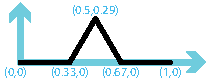
\includegraphics[scale=2]{images/KochParametric}
  \caption{Parametric coordinates for the Koch Snowflake shape.}
  \label{fig:KochParametric}
\end{figure}

Given these parametric coordinates, for each line we define an axis with the main axis along the line segment and the secondary axis perpendicular to that.
Given this definition, we can perform each fractal iteration by applying this transform for each line segment as shown in Figure~\ref{fig:KochApply}.

\begin{figure}[htb]
  \centering
  
\includegraphics[scale=2]{images/KochApply}
  \caption{Applying the line fractal transform for the Koch Snowflake.}
  \label{fig:KochApply}
\end{figure}

To implement the application of the line fractal demonstrated in Figure~\ref{fig:KochApply}, let us define a class named \textcode{LineFractalTransform} that takes as its constructor the coordinates of two ends of the original line.
As its operator, \textcode{LineFractalTransform} takes a point in parametric space and returns the coordinates in world space in respect to the original line segment.
We define this class in the \vtkmexec{} namespace because the intended use case is by worklets of the type we are making.
A definition of \textcode{LineFractalTransform} is given in Example~\ref{ex:LineFractalTransform}

\vtkmlisting[ex:LineFractalTransform]{A support class for a line fractal worklet.}{LineFractalTransform.h}

\begin{didyouknow}
  The definition of \textcode{LineFractalTransform} (or something like it) is not strictly necessary for implementing a worklet type.
  However, it is common to implement such supporting classes that operate in the execution environment in support of the operations typically applied by the worklet type.
\end{didyouknow}

The remainder of this chapter is dedicated to defining a \textcode{WorkletLineFractal} class and supporting objects that allow you to easily make line fractals.
Example~\ref{ex:KochSnowflake} demonstrates how we intend to use this worklet type.

\vtkmlisting[ex:KochSnowflake]{Demonstration of how we want to use the line fractal worklet.}{KochSnowflake.cxx}

\section{Thread Indices}
\label{sec:ThreadIndices}

\index{thread indices|(}

The first internal support class for implementing a worklet type is a class that manages indices for a thread.
As the name would imply, the thread indices class holds a reference to an index identifying work to be done by the current thread.
This includes indices to the current input element and the current output element.
The thread indices object can also hold other information (that may not strictly be index data) about the input and output data.
For example, the thread indices object for topology maps (named \vtkmexecarg{ThreadIndicesTopologyMap}) maintains cell shape and connection indices for the current input object.

As is discussed briefly in Section~\ref{sec:Fetch}, a thread indices object is given to the \vtkmexecarg{Fetch} class to retrieve data from the execution object.
The thread indices object serves two important functions for the \textidentifier{Fetch}.
The first function is to cache information about the current thread that is likely to be used by multiple objects retrieving information.
For example, in a point to cell topology map data from point fields must be retrieved by looking up indices in the topology connections.
It is more efficient to retrieve the topology connections once and store them in the thread indices than it is to look them up independently for each field.

The second function of thread indices is to make it easier to find information about the input domain when fetching data.
Once again, getting point data in a point to cell topology map requires looking up connectivity information in the input domain.
However, the \textidentifier{Fetch} object for the point field does not have direct access to the data for the input domain.
Instead, it gets this information from the thread indices.

All worklet classes have a method named \textcode{GetThreadIndices} that constructs a thread indices object for a given thread.
\textcode{GetThreadIndices} is called with 5 parameters: a unique index for the thread (i.e. worklet instance), an array portal that maps output indices to input indices (which might not be one-to-one if a scatter is being used), an array portal that gives the visit index for each output index, the execution object for the input domain, and an offset of the current index of the local invoke to a global indexing (used for streaming).

The base worklet implementation provides an implementation of \textcode{GetThreadIndices} that creates a \vtkmexecarg{ThreadIndicesBasic} object.
This provides the minimum information required in a thread indices object, but non-trivial worklet types are likely to need to provide their own thread indices type.
This following example shows the implementation of \textcode{GetThreadIndices} we will use in our worklet type superclass (discussed in more detail in Section~\ref{sec:NewWorkletTypes:WorkletSuperclass}).

\vtkmlisting[ex:GetThreadIndices]{Implementation of \textcode{GetThreadIndices} in a worklet superclass.}{GetThreadIndices.cxx}

As we can see in Example~\ref{ex:GetThreadIndices}, our new worklet type needs a custom thread indices class.
Specifically, we want the thread indices class to manage the coordinate information of the input line segment.

\begin{didyouknow}
  The implementation of a thread indices object we demonstrate here stores point coordinate information in addition to actual indices.
  It is acceptable for a thread indices object to store data that are not strictly indices.
  That said, the thread indices object should only load data (index or not) that is almost certain to be used by any worklet implementation.
  The thread indices object is created before any time that the worklet operator is called.
  If the thread indices object loads data that is never used by a worklet, that is a waste.
\end{didyouknow}

An implementation of a thread indices object usually derives from \vtkmexecarg{ThreadIndicesBasic} (or some other existing thread indices class) and adds to it information specific to a particular worklet type.

\vtkmlisting{Implementation of a thread indices class.}{ThreadIndicesLineFractal.h}

\index{thread indices|)}

\section{Signature Tags}
\label{sec:NewWorkletTypes:SignatureTags}

It is common that when defining a new worklet type, the new worklet type is associated with new types of data.
Thus, it is common that implementing new worklet types involves defining custom tags for \controlsignature{}s and \executionsignature{}s.
This in turn typically requires creating custom \textidentifier{TypeCheck}, \textidentifier{Transport}, and \textidentifier{Fetch} classes.

Chapter~\ref{chap:WorkletArguments} describes in detail the process of defining new worklet types and the associated code to manage data from an argument to the dispatcher's \textcode{Invoke} to the data that are passed to the worklet operator.
Rather than repeat the discussion, readers should review Chapter~\ref{chap:WorkletArguments} for details on how custom arguments are defined for a new worklet type.
In particular, we use the code from Examples \ref{ex:TypeCheckTag2DCoordinates} (page \pageref{ex:TypeCheckTag2DCoordinates}), \ref{ex:TransportImpl} (page \pageref{ex:TransportImpl}), and \ref{ex:FetchImplBasic} (page \pageref{ex:FetchImplBasic}) to implement an argument representing 2D line segments (which is our input domain).
All these examples culminate in the definition of a \controlsignature tag in our worklet superclass.

\vtkmlisting{Custom \protect\controlsignature tag for the input domain of our example worklet type.}{WorkletLineFractalInputDomainTag.cxx}

As you have worked with different existing worklet types, you have likely noticed that different worklet types have special \executionsignature tags to point to information in the input domain.
For example, a point to cell topology map has special \executionsignature tags for getting the input cell shape and the indices to all points incident on the current input cell.
We described in the beginning of the chapter that we wanted our worklet type to provide worklet implementations an object named \textcode{LineFractalTransform} (Example~\ref{ex:LineFractalTransform}), so it makes sense to define our own custom \executionsignature tag to provide this object.

Chapter~\ref{chap:WorkletArguments} gives an example of a custom \executionsignature tag that modifies what information is fetched from an argument (Examples \ref{ex:AspectImpl} and \ref{ex:CustomExecutionSignatureTag}).
However, \executionsignature tags that only pull data from input domain behave a little differently because they only get information from the thread indices object and ignore the associated data object.
This is done by providing a partial specialization of \vtkmexecarg{Fetch} that specializes on the aspect tag but not on the fetch tag.

\vtkmlisting[ex:InputDomainFetch]{A \textidentifier{Fetch} for an aspect that does not depend on any control argument.}{InputDomainFetch.h}

The definition of an associated \executionsignature tag simply has to use the define aspect as its \textcode{AspectTag}.
The tag also has to define a \textcode{INDEX} member (which is required of all \executionsignature tags).
This is problematic as this execution argument does not depend on any particular control argument.
Thus, it is customary to simply set the \textcode{INDEX} to 1.
There is guaranteed to be at least one \controlsignature argument for any worklet implementation.
Thus, the first argument is sure to exist and can then be ignored.

\vtkmlisting{Custom \protect\executionsignature tag that only relies on input domain information in the thread indices.}{WorkletLineFractalTransformTag.cxx}

One final implementation detail for our motivating example is that we need a \controlsignature tag to represent the output line segments to the worklet.
The use case has each worklet outputting a fixed number (greater than 1) of line segments for each input line segment.
To manage this, we will define another \controlsignature tag that outputs these line segments (as two \textidentifier{Vec}-2 coordinates).
This is defined as a \textidentifier{Vec} of \textidentifier{Vec}-2's.
The tag takes the number of line segments as a template argument.

\vtkmlisting[ex:WorkletLineFractalOutputTag]{Output \protect\controlsignature tag for our motivating example.}{WorkletLineFractalOutputTag.cxx}

You can see that the tag in Example~\ref{ex:WorkletLineFractalOutputTag} relies on a custom transport named \textcode{TransportTag2DLineSegmentsOut}.
There is nothing particularly special about this transport, but we provide the implementation here for completeness.

\vtkmlisting{Implementation of \textidentifier{Transport} for the output in our motivating example.}{TransportImpl2.h}

\section{Worklet Superclass}
\label{sec:NewWorkletTypes:WorkletSuperclass}
\label{sec:WorkletSuperclass}

The penultimate step in defining a new worklet type is to define a class that will serve as the superclass of all implementations of worklets of this type.
This class itself must inherit from \vtkmworkletinternal{WorkletBase}.
By convention the worklet superclass is placed in the \vtkmworklet{} namespace and its name starts with \textidentifier{Worklet}.

Within the worklet superclass we define the signature tags (as discussed in Section~\ref{sec:NewWorkletTypes:SignatureTags}) and the \textcode{GetThreadIndices} method (as discussed in Section~\ref{sec:ThreadIndices}.
The worklet superclass can also override other default behavior of the \textidentifier{WorkletBase} (such as special scatter).
And the worklet superclass can provide other items that might be particularly useful to its subclasses (such as commonly used tags).

\vtkmlisting[ex:WorkletSuperclass]{Superclass for a new type of worklet.}{WorkletLineFractal.h}

\begin{commonerrors}
  Be wary of creating worklet superclasses that are templated.
  The C++ compiler rules for superclass templates that are only partially specialized are non-intuitive.
  If a subclass does not fully resolve the template, features of the superclass such as signature tags will have to be qualified with \textcode{typename} keywords, which reduces the usability of the class.
\end{commonerrors}

\section{Dispatcher}
\label{sec:NewWorkletTypes:Dispatcher}

\index{dispatcher!creating new|(}

The final element required for a new worklet type is an associated dispatcher class for invoking the worklet.
As documented in Chapter~\ref{chap:Worklets}, each worklet type has its own associated dispatcher object.
By convention, the dispatcher is placed in the \vtkmworklet{} and has the same name as the worklet superclass with the \textidentifier{Worklet} replaced with \textidentifier{Dispatcher}.
So since the worklet superclass for our motivating example is named \textcode{WorkletLineFractal}, we name the associated dispatcher \textcode{DispatcherLineFractal}.

Also by convention, a dispatcher is a templated class.
The first template argument should be the type of the worklet (which should be a subclass of the associated worklet superclass).
The last template argument should be a device adapter tag with a default value set to \vtkmmacro{VTKM\_DEFAULT\_DEVICE\_ADAPTER\_TAG}.
Other template arguments that the dispatcher might need should be placed in between these two.

\vtkmlisting{Standard template arguments for a dispatcher class.}{DispatcherTemplate.cxx}

A dispatcher implementation inherits from \vtkmworkletinternal{DispatcherBase}.
\textidentifier{DispatcherBase} is itself a templated class with the following three templated arguments.
\begin{enumerate}
\item
  The dispatcher class that is subclassing \textidentifier{DispatcherBase}.
  All template arguments must be given.
\item
  The type of the worklet being dispatched (which by convention is the first argument of the dispatcher's template).
\item
  The expected superclass of the worklet, which is associated with the dispatcher implementation.
  \textidentifier{DispatcherBase} will check that the worklet has the appropriate superclass and provide a compile error if there is a mismatch.
\end{enumerate}

\begin{didyouknow}
  The convention of having a subclass be templated on the derived class' type is known as the Curiously Recurring Template Pattern (CRTP).
  In the case of \textidentifier{DispatcherBase}, \VTKm uses this CRTP behavior to allow the general implementation of \textcode{Invoke} to run \textcode{DoInvoke} in the subclass, which as we see in a moment is itself templated.
\end{didyouknow}

\vtkmlisting{Subclassing \textidentifier{DispatcherBase}.}{DispatcherSuperclass.cxx}

The constructor for the dispatcher should take as an argument an instance of the worklet to be invoked.
For convenience, this worklet argument should default to a new instance of the worklet.

\vtkmlisting{Typical constructor for a dispatcher.}{DispatcherConstructor.cxx}

Finally, the dispatcher must implement a const method named \textcode{DoInvoke}.
The \textcode{DoInvoke} method should take a single argument.
The argument will be an object of type \vtkminternal{Invocation} although it is usually more convenient to just express the argument type as a single template parameter.
The \textcode{Invocation} could contain several data items, so it is best to pass this argument as a constant reference.

\vtkmlisting{Declaration of \textcode{DoInvoke} of a dispatcher.}{DispatcherDoInvokePrototype.cxx}

\index{invocation object|(}
\index{dispatcher!invocation object|(}

\textidentifier{Invocation} is an object that encapsulates the state and data relevant to the invoke.
\textidentifier{Invocation} contains multiple types and data items.
For brevity only the ones most likely to be used in a \textcode{DoInvoke} method are documented here.
We discuss these briefly before getting back to the implementation of \textcode{DoInvoke}.

\vtkminternal{Invocation} contains a data member named \textcode{Parameters} that contains the data passed to the \textcode{Invoke} method of the dispatcher (with some possible transformations applied).
\textcode{Parameters} is stored in a \vtkminternal{FunctionInterface} template object.
(\textidentifier{FunctionInterface} is described in Chapter~\ref{chap:FunctionInterfaceObjects}.)
The specific type of \textcode{Parameters} is defined as type \textcode{ParameterInterface} in the \textidentifier{Invoke} object.

The \textidentifier{Invoke} object also contains the types \textcode{ControlInterface} and \textcode{ExecutionInterface} that are \textidentifier{FunctionInterface} classes built from the \controlsignature and \executionsignature of the worklet.
These \textidentifier{FunctionInterface} classes provide a simple mechanism for introspecting the arguments of the worklet's signatures.

All worklets must also define an input domain index, which points to one of the \controlsignature/\textidentifier{Invoke} arguments.
This number is also captured in the \vtkminternal{Invocation} object in a field named \textcode{InputDomainIndex}.
For convenience, \textidentifier{Invocation} also has the type \textcode{InputDomainTag} set to be the same as the \controlsignature argument corresponding to the input domain.
Likewise, \textidentifier{Invocation} has the type \textcode{InputDomainType} set to be the same type as the (transformed) input domain argument to \textcode{Invoke}.
\textidentifier{Invocation} also has a method name \textcode{GetInputDomain} that returns the invocation object passed to \textcode{Invoke}.

\index{dispatcher!invocation object|)}
\index{invocation object|)}

Getting back to the implementation of a dispatcher, the \textcode{DoInvoke} should first verify that the \controlsignature argument associated with the input domain is of the expected type.
This can be done by comparing the \textidentifier{Invocation}\textcode{::InputDomainTag} with the expected signature tag using a tool like \textcode{std::is\_same}.
This step is not strictly necessary, but is invaluable to users diagnosing issues with using the dispatcher.
It does not hurt to also check that the \textcode{Invoke} argument for the input domain is also the same as expected (by checking \textidentifier{Invocation}\textcode{::InputDomainType}).
It is additionally helpful to have a descriptive comment near these checks.

\vtkmlisting{Checking the input domain tag and type.}{CheckInputDomainType.cxx}

Next, \textcode{DoInvoke} must determine the size in number of elements of the input domain.
When the default identity scatter is used, the input domain size corresponds to the number of instances the worklet is executed.
(Other scatters will transform the input domain size to an output domain size, and that output domain size will determine the number of instances.)
The input domain size is generally determined by using \textidentifier{Invocation}::\textcode{::GetInputDomain} and querying the input domain argument.
In our motivating example, the input domain is an \textidentifier{ArrayHandle} and the input domain size is half the size of the array (since array entries are paired up into line segments).

The final thing \textcode{DoInvoke} does is call \textcode{BasicInvoke} on its \textidentifier{DispatcherBase} superclass.
\textcode{BasicInvoke} does the complicated work of transferring arguments, scheduling the parallel job, and calling the worklet's operator.
\textcode{BasicInvoke} takes three arguments: the \textidentifier{Invocation} object, the size of the input domain, and the device adapter tag to run on.

\vtkmlisting{Calling \textcode{BasicInvoke} from a dispatcher's \textcode{DoInvoke}.}{CallBasicInvoke.cxx}

Putting this all together, the following example demonstrates the full implementation of the dispatcher for our motivating example.

\vtkmlisting[ex:DispatcherImplementation]{Implementation of a dispatcher for a new type of worklet.}{DispatcherLineFractal.h}

\index{dispatcher!creating new|)}


\section{Using the Worklet}
\label{sec:NewWorkletTypes:Using}

Now that we have our full implementation of a worklet type that generates line fractals, let us have some fun with it.
The beginning of this chapter shows an implementation of the Koch Snowflake.
The remainder of this chapter demonstrates other fractals that are easily implemented with our worklet type.

\subsection{Quadratic Type 2 Curve}

There are multiple variants of the Koch Snowflake.
One simple but interesting version is the quadratic type 1 curve.
This fractal has a shape similar to what we used for Koch but has right angles and goes both up and down as shown in Figure~\ref{fig:QuadraticType2}.

\begin{figure}[htb]
  \centering
  
\includegraphics[scale=2]{images/QuadraticType2_1}
  \hfill
  
\includegraphics[scale=2]{images/QuadraticType2_2}
  \hfill
  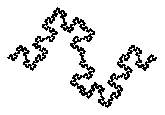
\includegraphics[scale=2]{images/QuadraticType2_4}
  \caption[The quadratic type 2 curve fractal.]{
    The quadratic type 2 curve fractal.
    The left image gives the first iteration.
    The middle image gives the second iteration.
    The right image gives the result after a few iterations.
  }
  \label{fig:QuadraticType2}
\end{figure}

The quadratic type 2 curve is implemented exactly like the Koch Snowflake except we output 8 lines to every input instead of 4, and, of course, the positions of the lines we generate are different.

\vtkmlisting{A worklet to generate a quadratic type 2 curve fractal.}{QuadraticType2.cxx}

\subsection{Tree Fractal}

Another type of fractal we can make is a tree fractal.
We will make a fractal similar to a Pythagoras tree except using lines instead of squares.
Our fractal will start with a vertical line that will be replaced with the off-center ``Y'' shape shown in Figure~\ref{fig:TreeFractal}.
Iterative replacing using this ``Y'' shape produces a bushy tree shape.

\begin{figure}[htb]
  \centering
  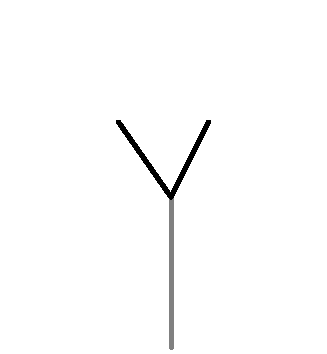
\includegraphics[scale=1]{images/Tree01}
  \hfill
  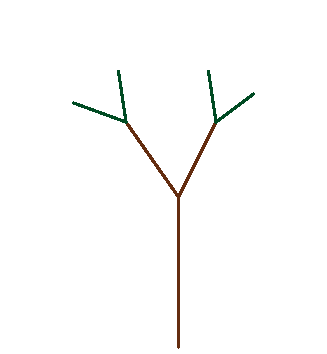
\includegraphics[scale=1]{images/Tree02}
  \hfill
  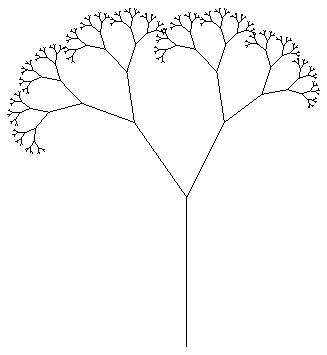
\includegraphics[scale=1]{images/Tree08}
  \caption[The tree fractal.]{
    The tree fractal replaces each line with the ``Y'' shape shown at left.
    An iteration grows branches at the end (middle).
    After several iterations the tree branches out to the bushy shape at right.
  }
  \label{fig:TreeFractal}
\end{figure}

One complication of implementing this tree fractal is that we really only want to apply the ``Y'' shape to the ``leaves'' of the tree.
For example, once we apply the ``Y'' to the trunk, we do not want to apply it to the trunk again.
If we were to apply it to the trunk again, we would create duplicates of the first layer of branches.

We can implement this feature in our worklet by using a count scatter.
(Worklet scatters are described in Section~\ref{sec:WorkletScatter}.)
Instead of directing the fractal worklet to generate 3 output line segments for every input line segment, we tell the fractal worklet to generate just 1 output line segment.
We then use a scatter counting to generate 3 line segments for the leaves and 1 line segment for all other line segments.
The count array for the initial iteration is initialized to a single 3.
Each iteration then creates the count array for the next iteration by writing a 1 for the base line segment and a 3 from the other two line segments.

\vtkmlisting{A worklet to generate a tree fractal.}{TreeFractal.cxx}

\subsection{Dragon Fractal}

\index{dragon fractal|(}

The next fractal we will implement is known as the dragon fractal.
The dragon fractal is also sometimes known as the \index{Heighway dragon}Heighway dragon or the \index{Harter-Heighway dragon}Harter-Heighway dragon after creators John Heighway, Bruce Banks, and William Harter.
It is also sometimes colloquially referred to as the \index{Jurassic Park dragon}Jurassic Park dragon as the fractal was prominently featured in the \textit{Jurassic Park} novel by Michael Crichton.

The basic building block is simple.
Each line segment is replaced by two line segments bent at 90 degrees and attached to the original segments endpoints as shown in Figure~\ref{fig:DragonFirst4}.
As you can see by the fourth iteration a more complicated pattern starts to emerge.
Figure~\ref{fig:Dragon12} shows the twelfth iteration a demonstrates a repeating spiral.

\begin{figure}[htb]
  \centering
  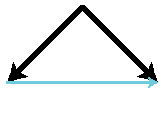
\includegraphics[scale=1.25]{images/Dragon01}
  \hfill
  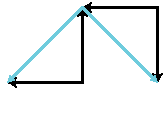
\includegraphics[scale=1.25]{images/Dragon02}
  \hfill
  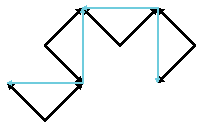
\includegraphics[scale=1.25]{images/Dragon03}
  \hfill
  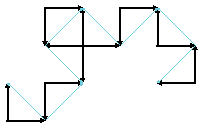
\includegraphics[scale=1.25]{images/Dragon04}
  \caption[The first four iterations of the dragon fractal.]{
    The first four iterations of the dragon fractal.
    The cyan lines give the previous iteration for reference.
  }
  \label{fig:DragonFirst4}
\end{figure}

What makes the dragon fractal different than the Koch Snowflake and similar fractals like the the quadratic curves implementation-wise is that the direction shape flips from one side to another.
Note in the second image of Figure~\ref{fig:DragonFirst4} the first bend is under the its associated line segment whereas the second is above its line segment.
The easiest way for us to control the bend is to alternate the direction of the line segments.
In Figure~\ref{fig:DragonFirst4} each line segment has an arrowhead indicating the orientation of the first and second point with the arrowhead at the second point.
Note that the shape is defined such that the first point of both line segments meet at the right angle.
With the shape defined this way, each iteration is applied to put the bend to the left of the segment with respect to an observer at the first point looking at the second point.

\begin{figure}[tbp]
  \centering
  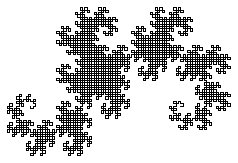
\includegraphics[width=\linewidth]{images/Dragon12}
  \caption{The dragon fractal after 12 iterations.}
  \label{fig:Dragon12}
\end{figure}

Other than reversing the direction of half the line segments, the implementation of the dragon fractal is nearly identical to the Koch Snowflake.

\vtkmlisting{A worklet to generate the dragon fractal.}{DragonFractal.cxx}

\index{dragon fractal|)}

\subsection{\fix{Hilbert Curve}}

\index{Hilbert curve|(}
\index{Hilbert curve|)}


\index{worklet types!creating new|)}


  % -*- latex -*-

\chapter{Advanced Worklet Customization}
\label{chap:AdvancedWorklets}

\fix{This chapter should be split up.}

Chapter~\ref{chap:Worklets} describes the basics of creating and using
worklets. Many visualization algorithms can be implemented using VTK-m's
existing worklet types and features. However, new algorithms and designs
may require features not provided by VTK-m's current worklet set. In such
cases it is possible to directly design filters using the lower level
device adapter operations \fix{as described in section bla}. But by adding
features to the worklet mechanisms, new designs can be integrated better
with the other VTK-m features and can be repurposed in interesting ways for
other algorithms.

This chapter provides the information necessary to create new mechanisms
for worklets. It first describes the interface for getting data from the
control environment objects to the data passed to a worklet invocation and
back. It then describes how to modify these mechanisms to create new data
movement structures and new worklet types.

\section{Transferring Arguments from Control to Execution}
\label{sec:TransferringArguments}

From the \controlsignature and \executionsignature defined in worklets,
VTK-m uses template meta-programming to build the code required to manage
data from control to execution environment. This management is handled by
three classes that provide type checking, transportation, and fetching.

\fix{I've been thinking that one more feature that these classes should
  provide is the ability to return the size of the domain. That would make
  things simpler and safer for getting the input domain size and checking
  the remaining domain sizes.}

\subsection{Type Checks}
\label{sec:TypeChecks}

\index{type~check|(}

Before attempting to move data from the control to the execution
environment, the VTK-m dispatchers check the input types to ensure that
they are compatible with the associated \controlsignature concept. This is
done with the \vtkmcontarg{TypeCheck} \textcode{struct}.

The \textidentifier{TypeCheck} \textcode{struct} is templated with two
parameters. The first parameter is a tag that identifies which check to
perform. The second parameter is the type of the control argument (after any
dynamic casts). The \textidentifier{TypeCheck} class contains a static
constant Boolean named \textcode{value} that is \textcode{true} if the type
in the second parameter is compatible with the tag in the first or
\textcode{false} otherwise.

Type checks are implemented with a defined type check tag (which, by
convention, is defined in the \vtkmcontarg{} namespace and starts with
\textcode{TypeCheckTag}) and a partial specialization of the
\vtkmcontarg{TypeCheck} structure. The following type checks (identified by
their tags) are provided in VTK-m.

\begin{description}
\item[\vtkmcontarg{TypeCheckTagArray}] \index{type~check!array} True if the
  type is a \vtkmcont{ArrayHandle}. \textidentifier{TypeCheckTagArray} also
  has a template parameter that is a type list. The
  \textidentifier{ArrayHandle} must also have a value type contained in
  this type list.
\item[\vtkmcontarg{TypeCheckTagExecObject}]
  \index{type~check!execution~object} True if the type is an execution
  object. All execution objects must derive from
  \vtkmexec{ExecutionObjectBase} and must be copyable through
  \textcode{memcpy} or similar mechanism.
\end{description}

Here are some trivial examples of using
\textidentifier{TypeCheck}. Typically these checks are done internally in
the base VTK-m dispatcher code, so these examples are for demonstration
only.

\vtkmlisting{Behavior of \protect\vtkmcontarg{TypeCheck}.}{TypeCheck.cxx}

\index{type~check|)}

\subsection{Transport}
\label{sec:Transport}

\index{transport|(}

After all the argument types are checked, the base dispatcher must load the
data into the execution environment before scheduling a job to run
there. This is done with the \vtkmcontarg{Transport} \textcode{struct}.

The \textidentifier{Transport} \textcode{struct} is templated with three
parameters. The first parameter is a tag that identifies which transport to
perform. The second parameter is the type of the control parameter (after any
dynamic casts). The third parameter is a device adapter tag for the device
on which the data will be loaded.

A \textidentifier{Transport} contains a \textcode{typedef} named \textcode{ExecObjectType} that is the type used after data is moved to the execution environment.
A \textidentifier{Transport} also has a \textcode{const} parenthesis operator that takes the control-side object that is to be transported to the execution environment, the control-side object that represents the input domain, and the size of the output domain and returns an execution-side object.
This operator is called in the control environment, and the returned object must be ready to be passed to the execution environment.

Transports are implemented with a defined transport tag (which, by
convention, is defined in the \vtkmcontarg{} namespace and starts with
\textcode{TransportTag}) and a partial specialization of the
\vtkmcontarg{Transport} structure. The following transports (identified by
their tags) are provided in VTK-m.

\begin{description}
\item[\vtkmcontarg{TransportTagArrayIn}] \index{transport!input~array}
  Loads data from a \vtkmcont{ArrayHandle} onto the specified device using
  the array handle's \textcode{PrepareForInput} method. The returned
  execution object is an array portal.
\item[\vtkmcontarg{TransportTagArrayOut}] \index{transport!output~array}
  Allocates data onto the specified device for a \vtkmcont{ArrayHandle}
  using the array handle's \textcode{PrepareForOutput} method. The returned
  execution object is an array portal.
\item[\vtkmcontarg{TransportTagExecObject}]
  \index{transport!execution~object} Simply returns the given execution
  object, which should be ready to load onto the device.
\end{description}

Here are some trivial examples of using
\textidentifier{Transport}. Typically this movement is done internally in
the base VTK-m dispatcher code, so these examples are for demonstration
only.

\vtkmlisting{Behavior of \protect\vtkmcontarg{Transport}.}{Transport.cxx}

\index{transport|)}

\subsection{Fetch}
\label{sec:Fetch}

\index{fetch|(}

Before the function of a worklet is invoked, the VTK-m internals pull the
appropriate data out of the execution object and pass it to the worklet
function. A class named \vtkmexecarg{Fetch} is responsible for pulling this
data out and putting computed data in to the execution objects.

The \textidentifier{Fetch} \textcode{struct} is templated with four
parameters. The first parameter is a tag that identifies which type of
fetch to perform. The second parameter is a different tag that identifies
the aspect of the data to fetch. The third parameter is an
\textidentifier{Invocation} type that provides details about how the
worklet is being dispatched including a list of execution object parameters
passed to the invocation. The fourth parameter is a \vtkm{IdComponent} that
points to the invocation parameter that the data should be fetched from.

A \textidentifier{Fetch} contains a \textcode{typedef} named
\textcode{ValueType} that is the type of data that is passed to and from
the worklet function. A \textidentifier{Fetch} also has a pair of methods
named \textcode{Load} and \textcode{Store} that get data from and add data
to the execution object at a given domain or thread index.

\index{aspect|(}
\index{fetch!aspect|see{aspect}}

Fetches are specified with a pair of fetch and aspect tags. Fetch tags are by
convention defined in the \vtkmexecarg{} namespace and start with
\textcode{FetchTag}. Likewise, aspect tags are also defined in the
\vtkmexecarg{} namespace and start with \textcode{AspectTag}. The
\textidentifier{Fetch} \textcode{typedef} is partially specialized on these
two tags.

\index{aspect!default} The most common aspect tag is
\vtkmexecarg{AspectTagDefault}, and all fetch tags should have a
specialization of \vtkmexecarg{Fetch} with this tag. The following list of
fetch tags describes the execution objects they work with and the data they
pull for each aspect tag they support.

\fix{Don't forget to add index entries for both fetch and aspect where
  appropriate.}

\begin{description}
\item[\vtkmexecarg{FetchTagArrayDirectIn}] \index{fetch!direct input array}
  Loads data from an array portal. This fetch only supports the
  \textidentifier{AspectTagDefault} aspect. The \textcode{Load} gets data
  directly from the domain (thread) index. The \textcode{Store} does
  nothing.
\item[\vtkmexecarg{FetchTagArrayDirectOut}] \index{fetch!direct output array}
  Stores data to an array portal. This fetch only supports the
  \textidentifier{AspectTagDefault} aspect. The \textcode{Store} sets data
  directly to the domain (thread) index. The \textcode{Load} does nothing.
\item[\vtkmexecarg{FetchTagExecObject}] \index{fetch!execution object}
  Simply returns an execution object. This fetch only supports the
  \textidentifier{AspectTagDefault} aspect. The \textcode{Load} returns the
  executive object in the associated parameter. The \textcode{Store} does
  nothing.
\end{description}

In addition to the aforementioned aspect tags that are explicitly paired
with fetch tags, VTK-m also provides some aspect tags that either modify
the behavior of a general fetch or simply ignore the type of fetch.

\begin{description}
\item[\vtkmexecarg{AspectTagWorkIndex}] \index{aspect!work index} Simply
  returns the domain (or thread) index ignoring any associated data. This
  aspect is used to implement the \sigtag{WorkIndex} execution signature
  tag.
\end{description}

\index{aspect|)}
\index{fetch|)}


\section{Function Interface Objects}
\label{sec:FunctionInterfaceObjects}

\index{function~interface|(}

For flexibility's sake a worklet is free to declare a \controlsignature
with whatever number of arguments are sensible for its operation. The
\textcode{Invoke} method of the dispatcher is expected to support arguments
that match these arguments, and part of the dispatching operation may
require these arguments to be augmented before the worklet is
scheduled. This leaves dispatchers with the tricky task of managing some
collection of arguments of unknown size and unknown types.

\fix{\textidentifier{FunctionInterface} is in the \vtkminternal{}
  interface. I still can't decide if it should be moved to the \vtkm{}
  interface.}

To simplify this management, VTK-m has the \vtkminternal{FunctionInterface}
class. \textidentifier{FunctionInterface} is a templated class that manages
a generic set of arguments and return value from a function. An instance of
\textidentifier{FunctionInterface} holds an instance of each argument. You
can apply the arguments in a \textidentifier{FunctionInterface} object to a
functor of a compatible prototype, and the resulting value of the function
call is saved in the \textidentifier{FunctionInterface}.

\subsection{Declaring and Creating}

\vtkminternal{FunctionInterface} is a templated class with a single
parameter. The parameter is the \index{function~signature}
\index{signature} \keyterm{signature} of the function. A signature is a
function type. The syntax in C++ is the return type followed by the
argument types encased in parentheses.

\vtkmlisting{Declaring \protect\vtkminternal{FunctionInterface}.}{DefineFunctionInterface.cxx}

The \vtkminternal{make\_FunctionInterface} function provies an easy way to
create a \textidentifier{FunctionInterface} and initialize the state of all
the parameters. \textidentifier{make\_FunctionInterface} takes a variable
number of arguments, one for each parameter. Since the return type is not
specified as an argument, you must always specify it as a template
parameter.

\vtkmlisting{Using \protect\vtkminternal{make\_FunctionInterface}.}{UseMakeFunctionInterface.cxx}

\subsection{Parameters}

One created, \textidentifier{FunctionInterface} contains methods to query
and manage the parameters and objects associated with them. The number of
parameters can be retrieved either with the constant field \index{arity}
\textcode{ARITY} or with the \textcode{GetArity} method.

\vtkmlisting{Getting the arity of a \textidentifier{FunctionInterface}.}{FunctionInterfaceArity.cxx}

To get a particular parameter, \textidentifier{FunctionInterface} has the
templated method \textcode{GetParameter}. The template parameter is the
index of the parameter. Note that the parameters in
\textidentifier{FunctionInterface} start at index 1. Although this is
uncommon in C++, it is customary to number function arguments starting at
1.

There are two ways to specify the index for \textcode{GetParameter}. The
first is to directly specify the template parameter (e.g.
\textcode{GetParameter<1>()}). However, note that in a templated function
or method where the type is not fully resolved the compiler will not
register \textcode{GetParameter} as a templated method and will fail to
parse the template argument without a \textcode{template} keyword. The
second way to specify the index is to provide a \vtkminternal{IndexTag}
object as an argument to \textcode{GetParameter}. Although this syntax is
more verbose, it works the same whether the
\textidentifier{FunctionInterface} is fully resolved or not. The following
example shows both methods in action.

\vtkmlisting{Using \textidentifier{FunctionInterface}\textcode{::GetParameter().}}{FunctionInterfaceGetParameter.cxx}

Likewise, there is a \textcode{SetParmeter} method for changing parameters.
The same rules for indexing and template specification apply.

\vtkmlisting{Using \textidentifier{FunctionInterface}\textcode{::SetParameter().}}{FunctionInterfaceSetParameter.cxx}

\subsection{Invoking}

\index{function~interface!invoke|(}

\textidentifier{FunctionInterface} can invoke a functor of a matching
signature using the parameters stored within. If the functor returns a
value, that return value will be stored in the
\textidentifier{FunctionInterface} object for later retrieval. There are
several versions of the invoke method. There are always seperate versions
of invoke methods for the control and execution environments so that
functors for either environment can be executed. The basic version of
invoke passes the parameters directly to the function and directly stores
the result.

\vtkmlisting{Invoking a \textidentifier{FunctionInterface}.}{FunctionInterfaceBasicInvoke.cxx}

Another form of the invoke methods takes a second transform functor that is
applied to each argument before passed to the main function. If the main
function returns a value, the transform is applied to that as well before
being stored back in the \textidentifier{FunctionInterface}.

\vtkmlisting{Invoking a \textidentifier{FunctionInterface} with a transform.}{FunctionInterfaceTransformInvoke.cxx}

\index{function~interface!invoke|)}

As demonstrated in the previous examples,
\textidentifier{FunctionInterface} has a method named
\textcode{GetReturnValue} that returns the value from the last invoke. Care
should be taken to only use \textcode{GetReturnValue} when the function
specification has a return value. If the function signature has a
\textcode{void} return type, using \textcode{GetReturnValue} will cause a
compile error.

\textidentifier{FunctionInterface} has an alternate method named
\textcode{GetReturnValueSafe} that returns the value wrapped in a templated
structure named \vtkminternal{FunctionInterfaceReturnContainer}. This
structure always has a static constant Boolean named \textcode{VALID} that
is \textcode{false} if there is no return type and \textcode{true}
otherwise. If the container is valid, it also has an entry named
\textcode{Value} containing the result.

\vtkmlisting{Getting return value from \textidentifier{FunctionInterface} safely.}{FunctionInterfaceReturnContainer.cxx}

\subsection{Modifying Parameters}

In addition to storing and querying parameters and invoking functions,
\textidentifier{FunctionInterface} also contains multiple ways to modify
the parameters to augment the function calls. This can be used in the same
use case as a chain of function calls that generally pass their parameters
but also augment the data along the way.

\index{function~interface!append parameter|(}

The \textcode{Append} method returns a new
\textidentifier{FunctionInterface} object with the same parameters plus a
new parameter (the argument to \textcode{Append}) to the end of the
parameters. There is also a matching \textcode{AppendType} templated
structure that can return the type of an augmented
\textidentifier{FunctionInterface} with a new type appended.

\vtkmlisting{Appending parameters to a \textidentifier{FunctionInterface}.}{FunctionInterfaceAppend.cxx}

\index{function~interface!append parameter|)}

\index{function~interface!replace parameter|(}

\textcode{Replace} is a similar method that returns a new
\textidentifier{FunctionInterface} object with the same paraemters except
with a specified parameter replaced with a new parameter (the argument to
\textcode{Replace}). There is also a matching \textcode{ReplaceType}
templated structure that can return the type of an augmented
\textidentifier{FunctionInterface} with one of the parameters replaced.

\vtkmlisting{Replacing parameters in a \textidentifier{FunctionInterface}.}{FunctionInterfaceReplace.cxx}

\index{function~interface!replace parameter|)}

It is sometimes desirable to make multiple modifications at a time. This
can be achieved by chaining modifications by calling \textcode{Append} or
\textcode{Replace} on the result of a previous call.

\vtkmlisting{Chaining \textcode{Replace} and \textcode{Append} with a \textidentifier{FunctionInterface}.}{FunctionInterfaceAppendAndReplace.cxx}

\subsection{Transformations}

Rather than replace a single item in a \textidentifier{FunctionInterface},
it is sometimes desirable to change them all in a similar
way. \textidentifier{FunctionInterface} supports two basic transform
operations on its parameters: a static transform and a dynamic
transform. The static transform determines its types at compile-time
whereas the dynamic transform happens at run-time.

\index{function~interface!static transform|(}

The static transform methods (named \textcode{StaticTransformCont} and
\textcode{StaticTransformExec}) operate by accepting a functor that defines
a function with two arguments. The first argument is the
\textidentifier{FunctionInterface} parameter to transform. The second
argument is an instance of the \vtkminternal{IndexTag} templated class that
statically identifies the parameter index being transformed. An
\textidentifier{IndexTag} object has no state, but the class contains a
static integer named \textidentifier{INDEX}. The function returns the
transformed argument.

The functor must also contain a templated class named \textcode{ReturnType}
with an internal type named \textcode{type} that defines the return type of
the transform for a given parameter type. \textcode{ReturnType} must have
two template parameters. The first template parameter is the type of the
\textidentifier{FunctionInterface} parameter to transform. It is the same
type as passed to the operator. The second template parameter is a
\vtkm{IdComponent} specifying the index.

The transformation is only applied to the parameters of the function. The
return argument is unaffected.

The return type can be determined with the \textcode{StaticTransformType}
template in the \textidentifier{FunctionInterface}
class. \textcode{StaticTransformType} has a single parameter that is the
transform functor and contains a type named \textcode{type} that is the
transformed \textidentifier{FunctionInterface}.

In the following example, a static transform is used to convert a
\textidentifier{FunctionInterface} to a new object that has the pointers to
the parameters rather than the values themselves. The parameter index is
always ignored as all parameters are uniformly transformed.

\vtkmlisting{Using a static transform of function interface class.}{FunctionInterfaceStaticTransform.cxx}

\index{function~interface!static transform|)}

\index{function~interface!dynamic transform|(}

There are cases where one set of parameters must be transformed to another
set, but the types of the new set are not known until run-time. That is,
the transformed type depends on the contents of the data. The
\textcode{DynamicTransformCont} method achieves this using a templated
callback that gets called with the correct type at run-time.

The dynamic transform works with two functors provided by the user code (as
opposed to the one functor in static transform). These functors are called
the transform functor and the finish functor. The transform functor accepts
three arguments. The first argument is a parameter to transform. The second
argument is a continue function. Rather than return the transformed value,
the transform functor calls the continue function, passing the transformed
value as an argument. The third argument is a \vtkminternal{IndexTag} for
the index of the argument being transformed.

Unlike its static counterpart, the dynamic transform method does not return
the transformed \textidentifier{FunctionInterface}. Instead, it passes the
transformed \textidentifier{FunctionInterface} to the finish functor passed
into \textcode{DynamicTransformCont}.

In the following contrived but illustrative example, a dynamic transform is
used to convert strings containing numbers into number arguments. Strings
that do not have numbers and all other arguments are passed through. Note
that because the types for strings are not determined till run-time, this
transform cannot be determined at compile time with meta-template
programming. The index argument is ignored because all arguments are
transformed the same way.


\vtkmlisting{Using a dynamic transform of a function interface.}{FunctionInterfaceDynamicTransform.cxx}

One common use for the \textidentifier{FunctionInterface} dynamic transform
is to convert parameters of virtual polymorphic type like
\vtkmcont{DynamicArrayHandle} and \vtkmcont{DynamicPointCoordinates}. This
use case is handled with a functor named
\vtkmcontinternal{DynamicTransform}. When used as the dynamic transform
functor, it will convert all of these dynamic types to their static
counterparts.

\vtkmlisting{Using \textidentifier{DynamicTransform} to cast dynamic arrays in a function interface.}{DynamicTransform.cxx}

\index{function~interface!dynamic transform|)}

\subsection{For Each}
\label{sec:FunctionInterface:ForEach}

\index{function~interface!for~each|(}

The invoke methods (principally) make a single function call passing all of
the parameters to this function. The transform methods call a function on
each parameter to convert it to some other data type. It is also sometimes
helpful to be able to call a unary function on each parameter that is not
expected to return a value. Typically the use case is for the function to
have some sort of side effect. For example, the function might print out
some value (such as in the following example) or perform some check on the
data and throw an exception on failure.

This feature is implemented in the for each methods of
\textidentifier{FunctionInterface}.  As with all the
\textidentifier{FunctionInterface} methods that take functors, there are
separate implementations for the control environment and the execution
environment. There are also separate implementations taking
\textcode{const} and non-\textcode{const} references to functors to
simplify making functors with side effects.

\vtkmlisting{Using the \textcode{ForEach} feature of \textidentifier{FunctionInterface}.}{FunctionInterfaceForEach.cxx}

\index{function~interface!for~each|)}

\index{function~interface|)}


\section{Invocation Objects}
\label{sec:InvocationObjects}


\section{Creating New \protect\controlsignature Tags}
\label{sec:NewControlSignatureTags}


\section{Creating New \protect\executionsignature Tags}
\label{sec:NewExecutionSignatureTags}


\section{Creating New Worklet Types}
\label{sec:NewWorkletTypes}

\subsection{New Worklet Superclasses}
\label{sec:NewWorkletSuperclasses}

\subsection{Dispatch Workflow}
\label{sec:DispatchWorkflow}

\subsection{New Dispatch Classes}
\label{sec:NewDispatchClasses}



}{}

\appendix
\part{Appendix}
\label{part:Appendix}
% -*- latex -*-

\chapter{Coding Conventions}
\label{chap:CodingConventions}

Several developers contribute to VTK-m and we welcome others who are
interested to also contribute to the project. To ensure readability and
consistency in the code, we have adopted the following coding
conventions. Many of these conventions are adapted from the coding
conventions of the VTK project. This is because many of the developers are
familiar with VTK coding and because we expect VTK-m to have continual
interaction with VTK.

\begin{itemize}
\item All code contributed to VTK-m must be compatible with VTK-m's BSD
  license.
\item Copyright notices should appear at the top of all source,
  configuration, and text files. The statement should have the following
  form (with the year replaced with the year the file was created):
\small\begin{verbatim}
//============================================================================
//  Copyright (c) Kitware, Inc.
//  All rights reserved.
//  See LICENSE.txt for details.
//  This software is distributed WITHOUT ANY WARRANTY; without even
//  the implied warranty of MERCHANTABILITY or FITNESS FOR A PARTICULAR
//  PURPOSE.  See the above copyright notice for more information.
//
//  Copyright 2014 Sandia Corporation.
//  Copyright 2014 UT-Battelle, LLC.
//  Copyright 2014. Los Alamos National Security
//
//  Under the terms of Contract DE-AC04-94AL85000 with Sandia Corporation,
//  the U.S. Government retains certain rights in this software.
//
//  Under the terms of Contract DE-AC52-06NA25396 with Los Alamos National
//  Laboratory (LANL), the U.S. Government retains certain rights in
//  this software.
//============================================================================
\end{verbatim}
  The \textfilename{CopyrightStatement} test checks all files for a similar
  statement. The test will print out a suggested text that can be copied
  and pasted to any file that has a missing copyright statement (with
  appropriate replacement of comment prefix). Exceptions to this copyright
  statement (for example, third-party files with different but compatible
  statements) can be added to \textfilename{LICENSE.txt}.
\item All include files should use include guards. starting right after the
  copyright statement. The naming convention of the include guard macro is
  that it should start with \textcode{vtk\_m} be followed with the path
  name, starting from the top-level source code directory under
  \textfilename{vtkm}, with non alphanumeric characters, such as
  \textcode{/} and \textcode{.} replaced with underscores. The
  \textcode{\#endif} part of the guard at the bottom of the file should
  include the guard name in a comment. For example, the
  \vtkmheader{vtkm/cont}{ArrayHandle.h} header contains the guard
\begin{verbatim}
#ifndef vtk_m_cont_ArrayHandle_h
#define vtk_m_cont_ArrayHandle_h
\end{verbatim}
  at the top and
\begin{verbatim}
#endif //vtk_m_cont_ArrayHandle_h
\end{verbatim}
\item VTK-m has several nested namespaces. The declaration of each
  namespace should be on its own line, and the code inside the namespace
  bracket should not be indented. The closing brace at the bottom of the
  namespace should be documented with a comment identifying the
  namespace. Namespaces can be grouped as desired. The following is a valid
  use of namespaces.
\begin{verbatim}
namespace vtkm {
namespace cont {

namespace detail {

class InternalClass;

} // namespace detail

class ExposedClass;

}
} // namespace vtkm::cont
\end{verbatim}
\item Multiple inheritance is not allowed in VTK-m classes.
\item Any functional public class should be in its own header file with the
  same name as the class. The file should be in a directory that
  corresponds to the namespace the class is in. There are several
  exceptions to this rule.
  \begin{itemize}
  \item Templated classes and template specialization often require the
    implementation of the class to be broken into pieces. Sometimes a
    specialization is placed in a header with a different name.
  \item Many VTK-m toolkit features are not encapsulated in
    classes. Functions may be collected by purpose or co-located with
    associated class.
  \item Although tags are technically classes, they behave as an
    enumeration for the compiler. Multiple tags that make up this
    enumeration are collected together.
  \item Some classes, such as \vtkm{Vec} are meant to behave as basic
    types. These are sometimes collected together as if they were related
    \textcode{typedef}s. The \vtkmheader{vtkm}{Types.h} header is a good
    example of this.
  \end{itemize}
\item The indentation follows the Allman style. The curly brace (scope
  delimiter) for a block is placed on the line following the prototype or
  control statement and is indented with the outer scope (i.e. the curly
  brace does not line up with the code in the block). This differs from VTK
  style, but was agreed on by the developers as the more common
  style. Indentations are two spaces.
\item Conditional clauses (including loop conditionals such as
  \textcode{for} and \textcode{while}) must be in braces below the
  conditional. That is, instead of
\begin{verbatim}
if (test) { clause; }
\end{verbatim}
  use
\begin{verbatim}
if (test)
{
  clause;
}
\end{verbatim}
  The rational for this requirement is to make it obvious whether the
  clause is executed when stepping through the code with the debugger. The
  one exception to this rule is when the clause contains a control-flow
  statement with obvious side effects such as \textcode{return} or
  \textcode{break}. However, even if the clause contains a single statement
  and is on the same line, the clause should be surrounded by braces.
\item Use two space indentation.
\item Tabs are not allowed. Only use spaces for indentation. No one can
  agree on what the size of a tab stop is, so it is better to not use them
  at all.
\item There should be no trailing whitespace in any line.
\item Use only alphanumeric characters in names. Use capitalization to
  demarcate words within a name (camel case). The exception is preprocessor
  macros and constant numbers that are, by convention, represented in all
  caps and a single underscore to demarcate words.
\item Namespace names are in all lowercase. They should be a single word
  that designates its meaning.
\item All class, method, member variable, and functions should start with a
  capital letter. Local variables should start in lower case and then use
  camel case. Exceptions can be made when such naming would conflict with
  previously established conventions in other library. (For example,
  \textcode{make\_ArrayHandle} corresponds to \textcode{make\_pair} in the
  standard template library.)
\item All class, function, and member names that have multiple words in
  their descriptions should be listed from general to specific. For
  example, if a class is a k-d tree that is used to locate points, the
  preferred name would be \textcode{LocatorPointKDTree}. This naming
  convention makes it easier to find both known and unknown classes in
  alphabetic lists.
\item Always spell out words in names; do not use abbreviations except in
  cases where the shortened form is widely understood and a name in its own
  right (e.g. OpenMP).
\item Always use descriptive names in all identifiers, including local
  variable names. Particularly avoid meaningless names of a few characters
  (e.g. \textcode{x}, \textcode{foo}, or \textcode{tmp}) or numbered names
  with no meaning to the number or order (e.g. \textcode{value1},
  \textcode{value2},\ldots). Also avoid the meaningless for loop variable
  names \textcode{i}, \textcode{j}, \textcode{k}, etc. Instead, use a name
  that identifies what type of index is being referenced such as
  \textcode{pointIndex}, \textcode{vertexIndex}, \textcode{componentIndex},
  etc.
\item Classes are documented with Doxygen-style comments before classes,
  methods, and functions.
\item Exposed classes should not have public instance variables outside of
  exceptional situations. Access is given by convention through methods
  with names starting with \textcode{Set} and \textcode{Get} or through
  overloaded operators.
\item References to classes and functions should be fully qualified with
  the namespace. This makes it easier to establish classes and functions
  from different packages and to find source and documentation for the
  referenced class. As an exception, if one class references an internal or
  detail class clearly associated with it, the reference can be shortened
  to \textcode{internal::} or \textcode{detail::}.
\item use \textcode{this->} inside of methods when accessing class methods
  and instance variables to distinguish between local variables and
  instance variables.
\item Include statements should generally be in alphabetical order. They
  can be grouped by package and type.
\item Namespaces should not be brought into global scope or the scope of
  any VTK-m package namespace with the ``using'' keyword. It should also be
  avoided in class, method, and function scopes (fully qualified namespace
  references are preferred).
\item All code must be valid by the C++11 specification.
\item Limit all lines to 80 characters whenever possible.
\item New code must include regression tests that will run on the
  dashboards. Generally a new class will have an associated ``UnitTest''
  that will test the operation of the test directly. There may be other
  tests necessary that exercise the operation with different components or
  on different architectures.
\item All code must compile and run without error or warning messages on
  the nightly dashboards, which should include Windows, Mac, and Linux.
\item Use \vtkm{Id} in lieu of \textcode{int} or \textcode{long} for data
  structure indices and \vtkm{IdComponent} for component indices of
  \vtkm{Vec} and related classes (like \vtkm{VecVariable} and
  \vtkm{Matrix}).
\item Whenever possible, use templates to resolve data types like
  \textcode{float}, \textcode{double}, or vectors to make code as flexible
  as possible. If a specific data type is required, prefer the
  VTK-m--provided types like \vtkm{Float32} and \vtkm{Float64} over the
  standard C types like \textcode{float} or
  \textcode{double}. \vtkm{FloatDefault} can be used in cases where there
  is no reasonable way to specify data precision (for example, when
  generating coordinates for uniform grids), but should be use sparingly.
\item All functions and methods defined within \VTKm should be
  declared with \vtkmcontmodifier, \vtkmexecmodifier, or \vtkmexeccontmodifier.
\end{itemize}

We should note that although these conventions impose a strict statute on
VTK-m coding, these rules (other than those involving licensing and
copyright) are not meant to be dogmatic. Examples can be found in the
existing code that break these conventions, particularly when the
conventions stand in the way of readability (which is the point in having
them in the first place). For example, it is often the case that it is more
readable for a complicated \textcode{typedef} to stretch a few characters
past 80 even if it pushes past the end of a display.



\backmatter
%\chapter{Index}
{\small
\printindex
}
\end{document}
